\documentclass[11pt,a4paper,onecolumn]{article}
%
\usepackage[top=30truemm,bottom=30truemm,left=25truemm,right=25truemm]{geometry}
\usepackage{amsmath,amssymb}
\makeatletter
\@addtoreset{equation}{section}
\def\theequation{\thesection.\arabic{equation}}
\makeatother
\usepackage{bm}
\usepackage[dvipdfmx]{graphicx}
\usepackage{ascmac}
\usepackage{longtable}
\usepackage{booktabs}
\usepackage{ltablex,booktabs}
\usepackage[dvipdfm,hidelinks]{hyperref}
%
\makeatletter
\def\maxwidth{\ifdim\Gin@nat@width>\linewidth\linewidth\else\Gin@nat@width\fi}
\def\maxheight{\ifdim\Gin@nat@height>\textheight\textheight\else\Gin@nat@height\fi}
\makeatother
% Scale images if necessary, so that they will not overflow the page
% margins by default, and it is still possible to overwrite the defaults
% using explicit options in \includegraphics[width, height, ...]{}
\setkeys{Gin}{width=\maxwidth,height=\maxheight,keepaspectratio}
%
\makeatletter
\renewcommand\paragraph{\@startsection{paragraph}{4}{\z@}%
                                    {3.25ex \@plus1ex \@minus.2ex}%
                                  {1.5ex \@plus .2ex}%
                                    %{-1em}%
                                    {\normalfont\normalsize\bfseries}}
\renewcommand\subparagraph{\@startsection{subparagraph}{5}{\parindent}%
                                       {3.25ex \@plus1ex \@minus .2ex}%
                                  {1.5ex \@plus .2ex}%
                                  %{-1em}%
                                      {\normalfont\normalsize\bfseries}}
\newcommand{\subsubsubsection}{\@startsection{paragraph}{4}{\z@}%
  {1.0\Cvs \@plus.5\Cdp \@minus.2\Cdp}%
  {1.5ex \@plus .2ex}%
  %{.1\Cvs \@plus.3\Cdp}%
{\reset@font\sffamily\normalsize}
}
\makeatother
\setcounter{secnumdepth}{4}
%
\pagenumbering{arabic}
%\usepackage{natbib} %全てのbibを表示
%
\begin{document}
  \begin{titlepage} % title page
    \topskip0pt
    \vspace*{\fill}
      \begin{center}
        {\Huge \textbf{Description of MIROC6 AGCM}}\\
        \vspace{100mm}
        {\Large \textbf{MIROC6 AGCM document writing team$^*$}}\\
        \vspace{30mm}
        {\Large \textbf{April 13, 2021}}
      \end{center}
    \vspace*{\fill}
    $^*${\bf\textbf{MIROC6 AGCM document writing team}} (in alphabetical order)
    \begin{quotation}
  Authors:
  Taigo Ando,
  Taro Higuchi,
  Haruka Hotta,
  Tomoki Iwakiri,
  Takuya Jinno,
  Kanon Kino,
  Yuki Takano,
  Masaki Toda,
  and
  Kazuya Yamazaki
\end{quotation}
\begin{quotation}
  Supervisors/Editors:
  Minoru Chikira,
  Takanori Kodama,
  Takuro Michibata,
  Hiroaki Miura,
  Tomoko Nitta,
  Tomoo Ogura,
  Fuyuki Saito,
  Miho Sekiguchi,
  Tatsuo
  Suzuki,
  Kentaroh Suzuki,
  Hiroaki Tatebe,
  Masahiro Watanabe,
  Shingo Watanabe,
  and
  Kei Yoshimura
\end{quotation}

  \end{titlepage}
%
  \clearpage
  \textbf{Remarks}

\hfill\break
\hfill\break
\hfill\break

How to cite

\begin{quote}
MIROC6 AGCM Document Writing Team (2021), Description of MIROC6 AGCM, CCSR Report No.~65, Division of Climate System Research, Atmosphere and Ocean Research Institute, The University of Tokyo.
doi:xxxxxx
\end{quote}

\hfill\break
\hfill\break
\hfill\break

Publisher Information

Division of Climate System Research,

Atmosphere and Ocean Research Institute,

The University of Tokyo

5-1-5, Kashiwanoha, Kashiwa-shi,

Chiba, 277-8568, Japan

Phone : 04-7136-4371 Fax : 04-7136-4375

Contact: Masahiro Watanabe (hiro@aori.u-tokyo.ac.jp)

\hfill\break
\hfill\break
\hfill\break
\hfill\break

\(\copyright\) 2021 MIROC6 AGCM document writing team

  \clearpage
  \textbf{Acknowledgment}

The original first version of this document was written in Japanese by
Dr.~Numaguti (deceased) in 1995 about the former version of the model,
CCSR/NIES AGCM5.4, which was created by himself. Since then, the AGCM
has been significantly upgraded with continuous community efforts, and
it has been periodically renamed by newer version number (e.g.,
CCSR/NIES AGCM5.6, MIROC3, MIROC4, and MIROC5) with almost the same
phases of releases of IPCC's Assessment Reports (TAR, AR4, and AR5).
Even though there are multiple published papers (e.g., K-1 model
developers (2004) for MIROC3 and Watanabe et al.~(2010) for MIROC5)
explained about the different versions of the model, the description
were made only for key points without details, and there were no major
updates of the original descriptive document by Dr.~Numaguti for a long
time.

Here, with the newest release of MIROC series, MIROC6(Tatebe et al.,
2019), it was decided to make an overhaul of the document for the first
time since the late 1990's. This decision was triggered by some
students' simple question: ``Why is this document so obsolete?'' Then,
under the TOUGOU project, some of the PIs organized the MIROC6 AGCM
document writing team in the spring of 2020.The team consists of two
groups; the authors and the supervisors/editors. All of the authors are
doctor course students of the University of Tokyo, who use or are
interested in using MIROC6, and the supervisors/editors are researchers,
who contributed to development of MIROC6 and/or its previous versions.

In the beginning, the team converted the original Japanese document
written in LaTeX format into English Markdown format. Ms.~Kino Kanon,
Ms.~Haruka Hotta, Mr.~Yuki Takano, and Dr.~Fuyuki Saito contributed to
make a semi-automated tool for this conversion. Then the team was
divided into several groups, and each group became in charge of each
section. These groups and corresponding sections are as follows:

\begin{itemize}
\item
  Mr.~Tomoki Iwakiri, Mr.~Masaki Toda, and Mr.~Kazuya Yamazaki
  supervised by Dr.~Fuyuki Saito for Dynamics (Ch.2) and Coupler Scheme
  (Ch.4.1)
\item
  Mr.~Yuki Takano supervised by Dr.~Minoru Chikira for Cumulus
  Scheme(Ch.3.2)
\item
  Mr.~Takuya Jinna supervised by Dr.~Tomoo Ogura for Shallow Convection
  Scheme (Ch.3.3)
\item
  Ms.~Haruka Hotta supervised by Dr.~Takuro Michibata and Dr.~Kentaro
  Suzuki for Large Scale Condensation (Ch.3.4) and Cloud Microphysics
  (Ch.3.5)
\item
  Mr.~Taro Higuchi supervised by Dr.~Takanori Kodama and Dr.~Miho
  Sekiguchi for Radiation Scheme (Ch.3.6)
\item
  Mr.~Taigo Ando supervised by Dr.~Minoru Chikira for Trubulence Scheme
  (Ch.3.7)
\item
  Ms.~Kanon Kino supervised by Dr.~Tatsuo Suzuki for Surface Flux
  Scheme(Ch.3.8)
\end{itemize}

It took about six months to draft, and the whole draft was reviewed by
all supervisors/editors. At last, the rest of the sections were amended
and improved by all. The team thanks the support of ``Integrated
Research Program for Advancing Climate Models (TOUGOU Program)'' from
the Ministry of Education, Culture, Sports, Science, and Technology
(MEXT), Japan.Finally, the team would sincerely express our respect and
condolences to Dr.~Numaguti, the first developer of the model and the
author of the original version of this document.

Hiroaki Tatebe, Masahiro Watanabe, and Kei Yoshimura lead member of the
teamMarch 31, 2021

  \clearpage
  \textbf{Revision History}

Text here.

	\tableofcontents
	\clearpage
	%
	\def\tightlist{\itemsep1pt\parskip0pt\parsep0pt}
	% please change the line below as your tex file (without ".tex")
	% agcm の概念と構造
  \hypertarget{model-overview.}{%
\section{Model Overview.}\label{model-overview.}}

\hypertarget{characteristics-of-ccsrnies-agcm}{%
\subsection{Characteristics of CCSR/NIES
AGCM}\label{characteristics-of-ccsrnies-agcm}}

AGCM5.4 was developed in collaboration with the Center for Climate
System Research (CCSR) at the University of Tokyo. Prepared in
collaboration with the National Institute for Environmental Studies
(NIES) , The model is a global three-dimensional general circulation
model. The features of the model are listed below.

\begin{longtable}[]{@{}ll@{}}
\toprule
\begin{minipage}[b]{0.47\columnwidth}\raggedright
Header0\strut
\end{minipage} & \begin{minipage}[b]{0.47\columnwidth}\raggedright
Header1\strut
\end{minipage}\tabularnewline
\midrule
\endhead
\begin{minipage}[t]{0.47\columnwidth}\raggedright
System of equations\strut
\end{minipage} & \begin{minipage}[t]{0.47\columnwidth}\raggedright
System of hydrostatic primitive equations\strut
\end{minipage}\tabularnewline
\begin{minipage}[t]{0.47\columnwidth}\raggedright
Area.\strut
\end{minipage} & \begin{minipage}[t]{0.47\columnwidth}\raggedright
Global 3D\strut
\end{minipage}\tabularnewline
\begin{minipage}[t]{0.47\columnwidth}\raggedright
Predictive variables\strut
\end{minipage} & \begin{minipage}[t]{0.47\columnwidth}\raggedright
\strut
\end{minipage}\tabularnewline
\begin{minipage}[t]{0.47\columnwidth}\raggedright
Horizontal Discretization\strut
\end{minipage} & \begin{minipage}[t]{0.47\columnwidth}\raggedright
Spectral Conversion Method\strut
\end{minipage}\tabularnewline
\begin{minipage}[t]{0.47\columnwidth}\raggedright
Vertical discretization\strut
\end{minipage} & \begin{minipage}[t]{0.47\columnwidth}\raggedright
σ system (Arakawa and Suarez, 1983)\strut
\end{minipage}\tabularnewline
\begin{minipage}[t]{0.47\columnwidth}\raggedright
Radiation\strut
\end{minipage} & \begin{minipage}[t]{0.47\columnwidth}\raggedright
2-stream DOM/adding method\strut
\end{minipage}\tabularnewline
\begin{minipage}[t]{0.47\columnwidth}\raggedright
\strut
\end{minipage} & \begin{minipage}[t]{0.47\columnwidth}\raggedright
(Based on Nakajima and Tanaka, 1986)\strut
\end{minipage}\tabularnewline
\begin{minipage}[t]{0.47\columnwidth}\raggedright
A large-scale cloud process\strut
\end{minipage} & \begin{minipage}[t]{0.47\columnwidth}\raggedright
Scheme with the total water mixing ratio as a forecast variable\strut
\end{minipage}\tabularnewline
\begin{minipage}[t]{0.47\columnwidth}\raggedright
\strut
\end{minipage} & \begin{minipage}[t]{0.47\columnwidth}\raggedright
(Based on Le Treut and Li, 1991)\strut
\end{minipage}\tabularnewline
\begin{minipage}[t]{0.47\columnwidth}\raggedright
Cumulus Convection\strut
\end{minipage} & \begin{minipage}[t]{0.47\columnwidth}\raggedright
Simplified Arakawa-Schubert scheme\strut
\end{minipage}\tabularnewline
\begin{minipage}[t]{0.47\columnwidth}\raggedright
Vertical Diffusion\strut
\end{minipage} & \begin{minipage}[t]{0.47\columnwidth}\raggedright
Mellor and Yamada(1974) level2\strut
\end{minipage}\tabularnewline
\begin{minipage}[t]{0.47\columnwidth}\raggedright
\strut
\end{minipage} & \begin{minipage}[t]{0.47\columnwidth}\raggedright
Louis (1979), bulk type\strut
\end{minipage}\tabularnewline
\begin{minipage}[t]{0.47\columnwidth}\raggedright
\strut
\end{minipage} & \begin{minipage}[t]{0.47\columnwidth}\raggedright
(Considering the convection effect of stomatal resistance, Miller et
al.~1992)\strut
\end{minipage}\tabularnewline
\begin{minipage}[t]{0.47\columnwidth}\raggedright
Surface Thermal Processes\strut
\end{minipage} & \begin{minipage}[t]{0.47\columnwidth}\raggedright
Multilayer Heat Transfer\strut
\end{minipage}\tabularnewline
\begin{minipage}[t]{0.47\columnwidth}\raggedright
Surface Hydrological Processes\strut
\end{minipage} & \begin{minipage}[t]{0.47\columnwidth}\raggedright
Bucket Model\strut
\end{minipage}\tabularnewline
\begin{minipage}[t]{0.47\columnwidth}\raggedright
\strut
\end{minipage} & \begin{minipage}[t]{0.47\columnwidth}\raggedright
\strut
\end{minipage}\tabularnewline
\begin{minipage}[t]{0.47\columnwidth}\raggedright
\strut
\end{minipage} & \begin{minipage}[t]{0.47\columnwidth}\raggedright
Scheme based on McFarlane (1987)\strut
\end{minipage}\tabularnewline
\begin{minipage}[t]{0.47\columnwidth}\raggedright
\strut
\end{minipage} & \begin{minipage}[t]{0.47\columnwidth}\raggedright
The north-south vertical and east-west vertical two-dimensional
models.\strut
\end{minipage}\tabularnewline
\bottomrule
\end{longtable}

\begin{verbatim}
The vertical one-dimensional model.
\end{verbatim}

\begin{itemize}
\item
  TAB00000: 18.0
\item
  TAB00000: 18.1\\
  The mixed-layer coupled model for the ocean
\end{itemize}

  \hypertarget{features-and-structure-of-the-model}{%
\subsection{Features and structure of the
model}\label{features-and-structure-of-the-model}}

\textbf{NOTE: the descriptions in this section are outdated.}

\hypertarget{basic-features-of-the-model.}{%
\subsubsection{Basic Features of the
Model.}\label{basic-features-of-the-model.}}

The MIROC6 AGCM is a numerical model for describing the global
three-dimensional atmosphere based on physical laws and calculating the
time evolution of the system as an initial value problem or a boundary
value problem.

The data to be inputted are as follows.

\begin{itemize}
\item
  Initial data for each prognostic variable (horizontal wind speed,
  temperature, surface pressure, specific humidity, cloud liquid water
  content, etc.)
\item
  Boundary condition data (surface elevation, surface condition, sea
  surface temperature, etc.)
\item
  Various parameters of the model (atmospheric components, physical
  process parameters, etc.)
\end{itemize}

On the other hand, the output is the following.

\begin{itemize}
\item
  Data for each prognostic parameter and diagnostic parameter, for each
  time or time average
\item
  Initial data to be used for continuous execution (restart data)
\item
  Progress and various diagnostic messages
\end{itemize}

The prognostic variable is the data obtained as a time series by
integrating the differential equation of time evolution, and the
diagnostic variable is the quantity calculated from the prognostic
variable, the boundary conditions and the parameters by some method that
does not include time integration.

More specifically, the model basically solves the following equations
(prognostic equations).

\begin{eqnarray}
  \frac{\partial{u}}{\partial {t}}  =  \left( {\mathcal F}_x \right)_D + \left( {\mathcal F}_x \right)_P.
   \\
  \frac{\partial{v}}{\partial {t}}  =  \left( {\mathcal F}_y \right)_D + \left( {\mathcal F}_y \right)_P. \\
  \frac{\partial{T}}{\partial {t}}  =  \left( Q \right)_D + \left( Q \right)_P. \\
  \frac{\partial{p_S}}{\partial {t}}  =  \left( M \right)_D + \left( M \right)_P. \\
  \frac{\partial{q}}{\partial {t}}  =  \left( S \right)_D + \left( S \right)_P. \\
  \frac{\partial{T_g}}{\partial {t}}  =  \left( Q_g \right)_D + \left( Q_g \right)_P.
\end{eqnarray}

Here, \(u,v,T,p_S,q,T_g\) are two-dimensional and three-dimensional
prognostic variables such as eastward wind, northward wind, temperature,
surface pressure, specific humidity, and surface state amount,
respectively, and the right-hand side is a term that causes time
variation of each prognostic variable. The terms
\({\mathcal F}_x,{\mathcal F}_y,Q,S,Q_g\) are calculated based on the
prognostic variables \(u,v,T,p_S,q,T_g\), are divided into two main
categories: the terms \(u\) and \(v\), such as advection due to the
motion of the atmosphere (the terms with index \(D\) in the above
equation), and the terms such as cloud and radiation (the terms with
index \(P\) in the above equation). There are two main types of terms.
The former is called the dynamical process, and the latter is called the
physical process.

The advection term is the main part of the time-varying term in
dynamical processes, and the accurate estimation of the spatial
derivative is important in its calculation. The MIROC6 AGCM utilizes the
spherical harmonic expansion to calculate the horizontal differential
term. On the other hand, it is important for physical processes to be
represented in a simple model with parameters (parameterization), such
as energy conversions due to the phase change of water, radiative
absorption and emission, the effects of small-scale atmospheric motions,
and the effects of various processes on the ground surface.

The time integration of the prognostic equation is done by approximating
the left-hand side of (1) etc. by the difference. For example,

\begin{eqnarray}
  \frac{\partial{q}}{\partial {t}} \rightarrow \frac{q^{t+\Delta t} - q^{t}}{\Delta t}
\end{eqnarray}

By making ,

\begin{eqnarray}
  q^{t+\Delta t} = q^{t}
       + \Delta t \left[ \left( S \right)_D + \left( S \right)_P  \right]
\end{eqnarray}

where \(S\) is a function of the prognostic variables \(u,v,T,p_S,q\).
Although \(S\) is a function of the prognostic variables
\(u,v,T,p_S,q\), and so on, there are various time difference schemes
that can be used in this calculation depending on the time of day the
prognostic variables are used to evaluate \(S\). The MIROC6 AGCM uses
the Euler method, which uses the value of the \(t\) as it is, the leap
frog method, which uses the value of the \(t+\Delta t/2\), and the
implicit method, which uses the (approximate) value of the
\(t+\Delta t\).

In the MIROC6 AGCM, the time integration of the prognostic variables is
done separately for the dynamical and physical processes. The dynamical
processes basically use a leap frog,

\begin{eqnarray}
  \tilde{q}^{t+\Delta t} = q^{t-\Delta t} + 2 \Delta t \left( S \right)_D^{t}
\end{eqnarray}

However, some terms are treated as implicit. In the physical process,
based on the results of integrating the dynamical terms, the Euler and
implicit methods are used together,

\begin{eqnarray}
  q^{t+\Delta t} = \tilde{q}^{t+\Delta t} + 2 \Delta t \left( S \right)_P
\end{eqnarray}

in (8). Note that \(\Delta t\) in (8) is replaced by \(2 \Delta t\).

\hypertarget{model-execution-flow.}{%
\subsubsection{Model Execution Flow.}\label{model-execution-flow.}}

The flow of the model execution is briefly shown below. The entries in
the index are the names of the corresponding subroutine.

\begin{enumerate}
\def\labelenumi{\arabic{enumi}.}
\item
  set the parameters of an experiment, coordinates, etc.
  \texttt{SUBROUTINE:{[}PCONST,ASETCO,SETPAR,SETTSTRT,SETTEND{]}}
\item
  read the initial values of the prognostic variables
  \texttt{SUBROUTINE:{[}RDSTRT{]}}
\item
  start the time step \texttt{SUBROUTINE:{[}TIMSTP{]}}
\item
  perform time integration by mechanical processes
  \texttt{SUBROUTINE:{[}DYNMCS{]}}
\item
  perform time integration by physical processes
  \texttt{SUBROUTINE:{[}PHYSCS{]}}
\item
  advance the time \texttt{MODULE:{[}TFILT{]}}
\item
  Output the data if necessary \texttt{MODULE:{[}HISTOU{]}}
\item
  Output the restart data if necessary \texttt{SUBROUTINE:{[}WRRSTR{]}}
\item
  Return to 3
\end{enumerate}

\hypertarget{prognostic-variables}{%
\subsubsection{Prognostic variables}\label{prognostic-variables}}

The prognostic variables are as follows. The values in parentheses are
the coordinate system, and \(\lambda,\varphi,\sigma, z\) indicate the
longitude, latitude, dimensionless pressure, \(\sigma\), and vertical
depth, respectively. The values in the square brackets are in units of
the index.

\setlength\LTleft{0pt}\setlength\LTright{0pt}\begin{longtable}[]{@{}lll@{}}
\toprule\relax
\begin{minipage}[b]{0.30\columnwidth}\raggedright
Element\strut
\end{minipage} & \begin{minipage}[b]{0.30\columnwidth}\raggedright
Symbol\strut
\end{minipage} & \begin{minipage}[b]{0.30\columnwidth}\raggedright
Unit\strut
\end{minipage}\tabularnewline
\midrule\relax
\endhead
\begin{minipage}[t]{0.30\columnwidth}\raggedright
eastward wind speed\strut
\end{minipage} & \begin{minipage}[t]{0.30\columnwidth}\raggedright
\(u\) (\(\lambda,\varphi,\sigma\))\strut
\end{minipage} & \begin{minipage}[t]{0.30\columnwidth}\raggedright
\(\mathrm{[m/s]}\)\strut
\end{minipage}\tabularnewline
\begin{minipage}[t]{0.30\columnwidth}\raggedright
northward wind speed\strut
\end{minipage} & \begin{minipage}[t]{0.30\columnwidth}\raggedright
\(v\) (\(\lambda,\varphi,\sigma\))\strut
\end{minipage} & \begin{minipage}[t]{0.30\columnwidth}\raggedright
\(\mathrm{[m/s]}\)\strut
\end{minipage}\tabularnewline
\begin{minipage}[t]{0.30\columnwidth}\raggedright
atmospheric temperature\strut
\end{minipage} & \begin{minipage}[t]{0.30\columnwidth}\raggedright
\(T\) (\(\lambda,\varphi,\sigma\))\strut
\end{minipage} & \begin{minipage}[t]{0.30\columnwidth}\raggedright
\(\mathrm{[K]}\)\strut
\end{minipage}\tabularnewline
\begin{minipage}[t]{0.30\columnwidth}\raggedright
surface pressure\strut
\end{minipage} & \begin{minipage}[t]{0.30\columnwidth}\raggedright
\(p_S\) (\(\lambda,\varphi\))\strut
\end{minipage} & \begin{minipage}[t]{0.30\columnwidth}\raggedright
\(\mathrm{[hPa]}\)\strut
\end{minipage}\tabularnewline
\begin{minipage}[t]{0.30\columnwidth}\raggedright
specific humidity\strut
\end{minipage} & \begin{minipage}[t]{0.30\columnwidth}\raggedright
\(q\) (\(\lambda,\varphi,\sigma\))\strut
\end{minipage} & \begin{minipage}[t]{0.30\columnwidth}\raggedright
\(\mathrm{[kg/kg]}\)\strut
\end{minipage}\tabularnewline
\begin{minipage}[t]{0.30\columnwidth}\raggedright
cloud water specific humidity\strut
\end{minipage} & \begin{minipage}[t]{0.30\columnwidth}\raggedright
\(l\) (\(\lambda,\varphi,\sigma\))\strut
\end{minipage} & \begin{minipage}[t]{0.30\columnwidth}\raggedright
\(\mathrm{[kg/kg]}\)\strut
\end{minipage}\tabularnewline
\begin{minipage}[t]{0.30\columnwidth}\raggedright
cloud ice specific humidity\strut
\end{minipage} & \begin{minipage}[t]{0.30\columnwidth}\raggedright
\(q_i\) (\(\lambda,\varphi,\sigma\))\strut
\end{minipage} & \begin{minipage}[t]{0.30\columnwidth}\raggedright
\(\mathrm{[kg/kg]}\)\strut
\end{minipage}\tabularnewline
\begin{minipage}[t]{0.30\columnwidth}\raggedright
total water PDF variance\strut
\end{minipage} & \begin{minipage}[t]{0.30\columnwidth}\raggedright
\(V\) (\(\lambda,\varphi,\sigma\))\strut
\end{minipage} & \begin{minipage}[t]{0.30\columnwidth}\raggedright
\(\mathrm{ND}\)\strut
\end{minipage}\tabularnewline
\begin{minipage}[t]{0.30\columnwidth}\raggedright
total water PDF skewness\strut
\end{minipage} & \begin{minipage}[t]{0.30\columnwidth}\raggedright
\(S\) (\(\lambda,\varphi,\sigma\))\strut
\end{minipage} & \begin{minipage}[t]{0.30\columnwidth}\raggedright
\(\mathrm{ND}\)\strut
\end{minipage}\tabularnewline
\begin{minipage}[t]{0.30\columnwidth}\raggedright
variance of liquid potential temperature\strut
\end{minipage} & \begin{minipage}[t]{0.30\columnwidth}\raggedright
\(TSQ\) (\(\lambda,\varphi,\sigma\))\strut
\end{minipage} & \begin{minipage}[t]{0.30\columnwidth}\raggedright
\(\mathrm{K^2}\)\strut
\end{minipage}\tabularnewline
\begin{minipage}[t]{0.30\columnwidth}\raggedright
covariance of liquid potential temperature and total water\strut
\end{minipage} & \begin{minipage}[t]{0.30\columnwidth}\raggedright
\(COV\) (\(\lambda,\varphi,\sigma\))\strut
\end{minipage} & \begin{minipage}[t]{0.30\columnwidth}\raggedright
\(\mathrm{K}\)\strut
\end{minipage}\tabularnewline
\begin{minipage}[t]{0.30\columnwidth}\raggedright
variance of total water\strut
\end{minipage} & \begin{minipage}[t]{0.30\columnwidth}\raggedright
\(QSQ\) (\(\lambda,\varphi,\sigma\))\strut
\end{minipage} & \begin{minipage}[t]{0.30\columnwidth}\raggedright
\(\mathrm{ND}\)\strut
\end{minipage}\tabularnewline
\begin{minipage}[t]{0.30\columnwidth}\raggedright
tracers\strut
\end{minipage} & \begin{minipage}[t]{0.30\columnwidth}\raggedright
\strut
\end{minipage} & \begin{minipage}[t]{0.30\columnwidth}\raggedright
\strut
\end{minipage}\tabularnewline
\bottomrule
\end{longtable}

Of these quantities, the quantities for turbulence process,
\(TSQ, COV, QSQ\), store only one step at a time, while the quantities
for the atmosphere, \(u, v, T, p_S, q, l, q_i, V, S\), need to store two
steps at a time. This is due to the fact that the leap frog method is
used in the time integration of the dynamic process of the quantities
related to the atmosphere.

The quantities of the atmosphere, \(u, v, T, p_S, q, l\), are variables
managed by the main routine,
\texttt{Administration\ of\ the\ Atmosphere\textquotesingle{}{[}AGCM5\textbackslash{}a{]}}.
On the other hand, the quantities relating to the earth's surface and
ground, \(q_i, V, S, TSQ, COV, QSQ\), do not appear in the main routine,
but are managed by the subroutine \texttt{MODULE:{[}PHYSCS{]}} of the
physical process.

Tracers include mass concentrations of aerosol species,

\hypertarget{the-flow-of-time-evolution-of-variables}{%
\subsubsection{The flow of time evolution of
variables}\label{the-flow-of-time-evolution-of-variables}}

This subsection is to be written.

	% 基本設定
	Basic Settings

Here we present the basic setup of the model.

\hypertarget{coordinate-system}{%
\subsubsection{Coordinate System}\label{coordinate-system}}

The coordinate system of the atmospheric model consists of longitude \(\lambda\), latitude \(\varphi\), and normalized pressure \(\eta\) (definitions are given below), each of which is treated as
orthogonal. However, \(z\) is used for the vertical coordinate in the ground, which is treated in a land physics component.

Longitude is discretized at equal intervals (\texttt{SUBROUTINE:~{[}SETLO{]}} in asetc.F).

\begin{eqnarray}
\begin{aligned}
\lambda_i = 2 \pi \frac{i-1}{I},  \;\;\; i = 1, \ldots I.\end{aligned}
\end{eqnarray}

Latitude grids \(\varphi_j\) are derived from the Gauss-Legendre integral formula (\texttt{SUBROUTINE:~{[}SETLA{]}} in asetc.F). This is the zero point of the Legendre polynomial of order J with
\(\mu = \sin \varphi\) as the argument (\texttt{SUBROUTINE:~{[}GAUSS{]}} in uspst.F). If J is large, we can approximate

\begin{eqnarray}
\begin{aligned}
\varphi_j =  \pi \left( \frac{1}{2}- \frac{j-1/2}{J} \right), \;\;\; j = 1, \ldots J.\end{aligned}
\end{eqnarray} Usually, the grid spacing of longitude and latitude is taken to be approximately equal to \(J = I/2\), based on the triangular truncation of the spectral method.

Air pressure \(p\) is defined at half-integer levels (\(p_{k+1/2},\ k = 1, 2, \ldots K\)) using the following formula using constants \(A_{k+1/2},\ B_{k+1/2}\):

\begin{eqnarray}
\begin{aligned}
p_{k+1/2} = A_{k+1/2} +B_{k+1/2}\,p_s,\end{aligned}
\end{eqnarray}

where \(A_{1/2}=A_{K+1/2}=0,\ B_{1/2}=1,\ B_{K+1/2}=0\) and thus \(p_{1/2}=p_s,\ p_{K+1/2}=0\). Therefore, the normalized pressure \(\sigma\equiv p/p_s\) can be written as below:

\begin{eqnarray}
\begin{aligned}
\sigma_{k+1/2} = \frac{A_{k+1/2}}{p_s} +B_{k+1/2}.\end{aligned}
\end{eqnarray}

Furthermore, a hybrid normalized pressure \(\eta\) is defined as below:

\begin{eqnarray}
\begin{aligned}
\eta_{k+1/2} = \frac{A_{k+1/2}}{p_0} +B_{k+1/2},\ \ \ p_0\equiv 1000\ \mathrm{hPa}.
\end{aligned}
\end{eqnarray}

Since \(A_{k+1/2},\ B_{k+1/2}, p_0\) are constants, \(\eta_{k+1/2}\) is also a constant and we use it as the vertical coordinate of the atmopheric model. However, as described in Chapter 2, basic
equations are descretized in such a way that \(\eta_{k+1/2}\) does not explicitly appear and \(\sigma_{k+1/2}\) is used instead to commonize source codes with the \(\sigma\)-coordinate system used in
MIROC 5.

Air pressure \(p_k\) at integer levels (\(p_k,\ k=1,2,\ldots K)\) is interpolated from half-level pressure as below:

\begin{eqnarray}
\begin{aligned}
p_k = \left\{ \frac{1}{1+\kappa}
\left( \frac{  p^{\kappa +1}_{k-1/2}
- p^{\kappa +1}_{k+1/2}      }
{ p_{k-1/2} - p_{k+1/2} }
\right)
\right\}^{1/\kappa}.
\end{aligned}
\end{eqnarray}

Full-level pressure in a 80-level configuration is shown in Fig. \ref{levels}. While lower layers follow the terrain, upper layers are isobaric, and the two are smoothly connected.

\begin{figure}
\centering
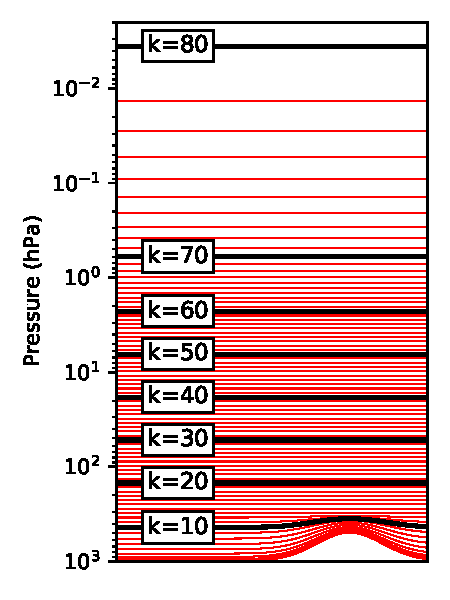
\includegraphics{../figures/levels.pdf}
\caption{Default arangement of vertical levels for 80-level simulations.}
\end{figure}

All prognostic variables are defined either on a grid of \((\lambda_i, \varphi_j, \eta_k)\) or \((\lambda_i, \varphi_j, z_l)\). (The underground level, \(z_l\), is described in the section on physical
processes.)

In the time direction, the prognostic equations are discretized at evenly spaced \(\Delta t\) and time integration is performed. However, \(\Delta t\) may change in cases where the stability of the
time integration is insufficient.

\hypertarget{physical-constants}{%
\subsubsection{Physical Constants}\label{physical-constants}}

The basic physical constants are shown below (\texttt{SUBROUTINE~{[}PCONST{]}} in apcon.F).

\begin{eqnarray}
\begin{array}{llll}
\hline \text { Element } & \text { Symbol } & \text { Unit } & \text { Value } \\
\hline \text { Earth radius } & a & \mathrm{~m} & 6.37 \times 10^{6} \\
\text { Gravitational acceleration } & g & \mathrm{~m} \mathrm{~s}^{-2} & 9.8 \\
\text { Atmospheric specific heat at constant pressure } & C_{p} & \mathrm{~J} \mathrm{~kg}^{-1} \mathrm{~K}^{-1} & 1004.6 \\
\text { Atmospheric gas constant } & R & \mathrm{~J} \mathrm{~kg}^{-1} \mathrm{~K}^{-1} & 287.04 \\
\text { Latent heat of water evaporation } & L & \mathrm{~J} \mathrm{~kg}^{-1} & 2.5 \times 10^{6} \\
\text { Water vapor specific heat at constant pressure } & C_{v} & \mathrm{~J} \mathrm{~kg}^{-1} \mathrm{~K}^{-1} & 1810 \\
\text { Gas constant of water } & R_{v} & \mathrm{~J} \mathrm{~kg}^{-1} \mathrm{~K}^{-1} & 461 \\
\text { Density of liquid water } & d_{H_{2} O} & \mathrm{~kg} \mathrm{~m}^{-3} & 1000 \\
\text { Saturated vapor pressure at } 0{ }^{\circ} \mathrm{C} & e^{*}(273 \mathrm{~K}) & \mathrm{Pa} & 611 \\
\text { Stefan-Bolzman constant } & \sigma_{S B} & \mathrm{~W} \mathrm{~m}^{-2} \mathrm{~K}^{-4} & 5.67 \times 10^{-8} \\
\text { Kárman constant } & k & & 0.4 \\
\text { Latent heat of ice melting } & L_{M} & \mathrm{~J} \mathrm{~kg}^{-1} & 3.4 \times 10^{5} \\
\text { Freezing point of water } & T_{M} & \mathrm{~K} & 273.15 \\
\text { Constant pressure specific heat of water } & C_{w} & \mathrm{~J} \mathrm{~kg}^{-1} & 4200 \\
\text { Freezing point of seawater } & T_{I} & \mathrm{~K} & 271.35 \\
\text { Specific heat ratio of ice at constant pressure } & C_{I}=C_{w}-L_{M} / T_{M} & & 2397 \\
\text { Water vapor molecular weight ratio } & \epsilon=R / R_{v} & & 0.622 \\
\text { Coefficient of virtual temperature } & \epsilon_{v}=\epsilon^{-1}-1 & & 0.606 \\
\text { Ratio of specific heat to gas constant } & \kappa=R / C_{p} & & 0.286 \\
\hline
\end{array}
\end{eqnarray}

	% Computational flow of dynamical core
	\hypertarget{dynamics}{%
\section{Dynamics}\label{dynamics}}

\hypertarget{basic-equations}{%
\subsection{Basic Equations}\label{basic-equations}}

\hypertarget{basic-equations-1}{%
\subsubsection{Basic Equations}\label{basic-equations-1}}

The basic equations are a system of primitive equations at the spherical
(\(\lambda,\varphi\)) and \(\eta\) coordinates, given as follows
(Arakawa and Konor 1996).

\begin{enumerate}
\def\labelenumi{\arabic{enumi}.}
\tightlist
\item
  Continuity equation
\end{enumerate}
\begin{eqnarray}
  \frac{\partial m}{\partial t}
    + \nabla_{\eta} \cdot (m\mathbf{v}_H)+ \frac{\partial (m\dot{\eta})}{\partial \eta} = 0
\end{eqnarray}

\begin{enumerate}
\def\labelenumi{\arabic{enumi}.}
\setcounter{enumi}{1}
\tightlist
\item
  Hydrostatic equation
\end{enumerate}
\begin{eqnarray}
  \frac{\partial \Phi}{\partial \eta} = - \frac{RT_v}{p} m
\end{eqnarray}

\begin{enumerate}
\def\labelenumi{\arabic{enumi}.}
\setcounter{enumi}{2}
\tightlist
\item
  Equation of motion
\end{enumerate}
\begin{eqnarray}
  \frac{\partial \zeta}{\partial t} 
     =   \frac{1}{a\cos\varphi}
            \frac{\partial A_v}{\partial \lambda}
          - \frac{1}{a\cos \varphi}
            \frac{\partial}{\partial \varphi} ( A_u \cos\varphi )
          - {\mathcal D}(\zeta) 
\end{eqnarray}
\begin{eqnarray}
  \frac{\partial D}{\partial t} 
     =    \frac{1}{a\cos\varphi}
            \frac{\partial A_u}{\partial \lambda}
          + \frac{1}{a\cos\varphi}
            \frac{\partial }{\partial \varphi} ( A_v \cos\varphi )
          - \nabla^{2}_{\eta}
           ( \Phi + R \bar{T} \pi + E ) 
          - {\mathcal D}(D) 
\end{eqnarray}

\begin{enumerate}
\def\labelenumi{\arabic{enumi}.}
\setcounter{enumi}{3}
\tightlist
\item
  Thermodynamic equation
\end{enumerate}
\begin{eqnarray}
  \frac{\partial T}{\partial t}
     &=&  - \frac{1}{a\cos\varphi}
               \frac{\partial uT'}{\partial \lambda}
          - \frac{1}{a}
               \frac{\partial }{\partial \varphi} ( vT' \cos\varphi )
          + T' D \\
        &-& \dot{\eta} 
              \frac{\partial T }{\partial \eta}
          + \frac{\kappa T}{\sigma} \left[ B\left( \frac{\partial \pi}{\partial t}
                            + {\mathbf{v}}_{H} \cdot \nabla_{\eta}\pi \right)
                            + \frac{ m\dot{\eta} }{ p_s }
                     \right]
          + \frac{Q}{C_{p}}
          + \frac{Q_{diff}}{C_{p}}
          - {\mathcal D}(T) 
\end{eqnarray}

\begin{enumerate}
\def\labelenumi{\arabic{enumi}.}
\setcounter{enumi}{4}
\tightlist
\item
  Tracers
\end{enumerate}

For any tracer whose mixing ratio is denoted as \(q\),
\begin{eqnarray}
  \frac{\partial q}{\partial t}
   &=&  - \frac{1}{a\cos\varphi}
               \frac{\partial uq}{\partial \lambda}
          - \frac{1}{a\cos\varphi}
               \frac{\partial }{\partial \varphi} (vq \cos\varphi)
          + q D \\
        &-& \dot{\eta} \frac{\partial q }{\partial \eta}
          + S_{q}
          - {\mathcal D}(q) 
\end{eqnarray}

Here,
\begin{eqnarray}
m &\equiv & \left(\frac{\partial p}{\partial \eta}\right)_{p_s}, \\
\theta  &\equiv &  T \left( p/p_{0} \right)^{-\kappa}, \\
\kappa  &\equiv &  R/C_{p}, \\
  \Phi  &\equiv &  gz, \\
   \pi  &\equiv &  \ln p_{S}, \\
 \dot{\eta}  &\equiv &   \frac{\mathrm{d}\eta}{\mathrm{d}t}, \\
     T_v  &\equiv &  T ( 1+\epsilon_v q ), \\
     T  &\equiv &   \bar{T} + T^{\prime}, \\
     \bar{T}&\equiv & 300 \ \mathrm{K}, \\
 \zeta  &\equiv &  \frac{1}{a \cos\varphi }
                    \frac{\partial v}{\partial \lambda} 
             -    \frac{1}{a \cos\varphi }
                    \frac{\partial }{\partial \varphi}
                    ( u \cos\varphi ), \\
     D  &\equiv &  \frac{1}{a \cos\varphi }
                    \frac{\partial u}{\partial \lambda} 
             +    \frac{1}{a \cos\varphi }
                    \frac{\partial }{\partial \varphi}
                    ( v \cos\varphi ), \\
    A_u  &\equiv &   ( \zeta + f ) v
             - \dot{\eta} \frac{\partial u}{\partial \eta} 
             - \frac{RT^{\prime}}{a\cos\varphi} 
                  \frac{\partial \pi}{\partial \lambda} 
             + {\mathcal F}_x, \\
    A_v  &\equiv &  - ( \zeta + f ) u
             - \dot{\eta} \frac{\partial v}{\partial \eta} 
             - \frac{RT^{\prime}}{a}
                  \frac{\partial \pi}{\partial \varphi} 
             + {\mathcal F}_y, \\
     E  &\equiv &   \frac{u^{2}+v^{2}}{2}, \\
 {\mathbf{v}}_{H} \cdot \nabla
        &\equiv &  \frac{u}{a \cos \varphi} 
         \left( \frac{\partial }{\partial \lambda} \right)_{\sigma}
     + \frac{v}{a}
         \left( \frac{\partial }{\partial \varphi} \right)_{\sigma}, \\
  \nabla^{2}_{\eta}  
        &\equiv &  
               \frac{1}{a^{2}\cos^2\varphi} 
                 \frac{\partial^{2} }{\partial \lambda^{2}} 
             + \frac{1}{a^{2}\cos\varphi} 
                 \frac{\partial }{\partial \varphi}
                 \left[ \cos\varphi
                       \frac{\partial }{\partial \varphi} \right].
\end{eqnarray}

\({\mathcal D}(\zeta), {\mathcal D}(D), {\mathcal D}(T), {\mathcal D}(q)\)
are horizontal diffusion terms,
\({\mathcal F}_\lambda, {\mathcal F}_\varphi\) are forces due to
small-scale kinetic processes (treated as `physical processes'), \(Q\)
are forces due to radiation, condensation, small-scale kinetic
processes, etc. Heating and temperature change due to `physical
processes', and \(S_q\) is a water vapor source term due to `physical
processes' such as condensation and small-scale motion. \(Q_{diff}\) is
the heat of friction and
\begin{eqnarray}
  Q_{diff}
 = - {\mathbf{v}} \cdot  ( \frac{\partial {\mathbf{v}}}{\partial t} )_{diff} .
\end{eqnarray}

\(( \frac{\partial {\mathbf{v}}}{\partial t} )_{diff}\) is a
time-varying term of \(u,v\) due to horizontal and vertical diffusion.

\hypertarget{boundary-conditions}{%
\subsubsection{Boundary Conditions}\label{boundary-conditions}}

Upper and lower boundary conditions for the vertical velocity is:
\begin{eqnarray}
  \dot{\eta} = 0  \ \ \ at \ \ \eta = 0 , \ 1 .
\end{eqnarray}
The prognostic equation for \(p_s\) and the diagnostic equation for the
vertical velocity can be derived by integrating the continuity equation
and applying these boundary conditions.

	\hypertarget{vertical-discretization}{%
\subsection{Vertical Discretization}\label{vertical-discretization}}

Following Arakawa and Konor (1996) but in the Lorentz grid, the basic
equations are discretized vertically by differences. This scheme has the
following characteristics.

\begin{itemize}
\item
  Save the total integrated mass
\item
  Save the total integrated energy
\item
  Preserving angular momentum for global integration
\item
  Conservation of total mass-integrated potential temperature
\item
  The hydrostatic pressure equation comes down to local (the altitude of
  the lower level is independent of the temperature of the upper level)
\item
  For a given temperature distribution, constant in the horizontal
  direction, the hydrostatic pressure equation becomes accurate and the
  barometric gradient force becomes zero.
\item
  Isothermal atmosphere stays isothermal forever
\end{itemize}

\hypertarget{model-levels}{%
\subsubsection{Model levels}\label{model-levels}}

Model level increases in altitude with the vertical level number $k$. $k=1/2$ corresponds with the model bottom (\(\eta=1\)), while $k=K+1/2$ corresponds to the model top ($\eta=0$).
Variables $\zeta,D,T,q$ are defined at full levels ($k=1,2,\ldots K$), while the vertical velocity $\dot{\eta}$ is defined at half levels ($k=1/2,3/2,\ldots K+1/2$).
Using constants $A_{k+1/2}$ and $B_{k+1/2}$ and variable surface pressure $p_s$, air pressure at half levels are defined as below:
\begin{eqnarray}
p_{k+1/2} = A_{k+1/2} +B_{k+1/2}\,p_s.
\end{eqnarray}

Thus, the normalized pressure \(\sigma\equiv p/p_s\) can be written as below:
\begin{eqnarray}
\sigma_{k+1/2} = \frac{A_{k+1/2}}{p_s} +B_{k+1/2}.
\end{eqnarray}

Using a reference pressure \(p_0=1000\ \mathrm{hPa}\), the hybrid-normalized pressure \(\eta\) is defined as below:
\begin{eqnarray}
\eta_{k+1/2} = \frac{A_{k+1/2}}{p_0} +B_{k+1/2},
\end{eqnarray}
which is a constant at all levels and is used as the vertical coordinate by default in MIROC 6.0.

Pressure at full levels are interpolated from half-level pressure by the following formula:
\begin{eqnarray}
 p_k = \left\{ \frac{1}{1+\kappa}
                     \left( \frac{  p^{\kappa +1}_{k-1/2}
                                  - p^{\kappa +1}_{k+1/2}      }
                                  { p_{k-1/2} - p_{k+1/2} }
                     \right)
              \right\}^{1/\kappa}.
\end{eqnarray}

For later use, let us define the following:
\begin{eqnarray}
  \Delta\sigma_k &\equiv & \sigma_{k-1/2} - \sigma_{k+1/2}, \\
  \Delta B_k &\equiv & B_{k-1/2} - B_{k+1/2}.
\end{eqnarray}

\hypertarget{vertical-discretization-1}{%
\subsubsection{Vertical
discretization}\label{vertical-discretization-1}}

Basic equations vertically discretized at the $\eta$ hybrid coordinates are shown below.

\begin{enumerate}
\def\labelenumi{\arabic{enumi}.}
\tightlist
\item
  Continuity equation and diagnosis of the vertical velocity
\end{enumerate}
\begin{eqnarray}
  \frac{\partial \pi}{\partial t}
 = - \sum_{k=1}^{K} \left\{ D_k \Delta\sigma_k + ({\mathbf{v}}_k \cdot \nabla \pi)\Delta B_k \right\}
\end{eqnarray}

In MIRCO 6.0, the discretization is conducted in a manner similar to the $\sigma$ coordinate,
which can be optionally selected and was the default in previous versions, to commonize source codes.
Thus, the vertical velocity is represented as \(\dot{\sigma}=m\dot{\eta}/p_s\).
Furthermore, vertical advection \(\dot{\eta}(\partial/\partial\eta)\) is replaced with an equivalent form \(m\dot{\eta}/p_s(\partial/\partial\sigma)\).
\begin{eqnarray}
  \left(\dot{\sigma}=\right)\frac{(m\dot{\eta})_{k-1/2}}{p_s}
 = - B_{k-1/2} \frac{\partial \pi}{\partial t}
   - \sum_{l=k}^{K}\left\{ D_l \Delta\sigma_l + ({\mathbf{v}}_l \cdot \nabla \pi)\Delta B_l \right\}
\end{eqnarray}
\begin{eqnarray}
  \frac{(m\dot{\eta})_{1/2}}{p_s} = \frac{(m\dot{\eta})_{k+1/2}}{p_s} = 0
\end{eqnarray}

\begin{enumerate}
\def\labelenumi{\arabic{enumi}.}
\setcounter{enumi}{1}
\tightlist
\item
  Hydrostatic equation
\end{enumerate}
\begin{eqnarray}
 \Phi_{1}  &=&  \Phi_{s} + C_{p} ( \sigma_{1}^{-\kappa} - 1  ) T_{v,1} \\
           &=&  \Phi_{s} + C_{p} \alpha_{1} T_{v,1} 
\end{eqnarray}
\begin{eqnarray}
 \Phi_k - \Phi_{k-1} 
  &=&  C_{p}
   \left[ \left( \frac{ p_{k-1/2} }{ p_k } \right)^{\kappa}
          - 1 \right] T_{v,k} 
       + C_{p}
   \left[ 1- 
         \left( \frac{ p_{k-1/2} }{ p_{k-1} } \right)^{\kappa}
              \right] T_{v,k-1} \\
   &=&    C_{p} \alpha_k T_{v,k} + C_{p} \beta_{k-1} T_{v,k-1}
\end{eqnarray}
Here,
\begin{eqnarray}
 \alpha_k &\equiv & \left( \frac{ p_{k-1/2} }
                               { p_k } \right)^{\kappa} -1, \\
 \beta_k &\equiv &  1- \left( \frac{ p_{k+1/2} }
                               { p_k } \right)^{\kappa} .
\end{eqnarray}

\begin{enumerate}
\def\labelenumi{\arabic{enumi}.}
\setcounter{enumi}{2}
\tightlist
\item
  Equations of motion
\end{enumerate}
\begin{eqnarray}
  \frac{\partial \zeta_k}{\partial t} 
        &=&   \frac{1}{a\cos\varphi} 
            \frac{\partial (A_v)_k}{\partial \lambda}
          - \frac{1}{a\cos\varphi} 
            \frac{\partial }{\partial \varphi} (A_u \cos\varphi)_k
          - {\mathcal D}(\zeta_k) \\
  \frac{\partial D}{\partial t} 
        &=&   \frac{1}{a\cos\varphi} 
            \frac{\partial (A_u)_k}{\partial \lambda}
          + \frac{1}{a\cos\varphi} 
            \frac{\partial }{\partial \varphi} (A_v \cos\varphi)_k
          - \nabla^{2}_{\eta}
           ( \Phi_k + R\bar{T} \pi 
             + ({\mathit KE})_k )
          - {\mathcal D}(D_k) \\
  (A_u)_k
    &=&  ( \zeta_k + f ) v_k 
             - \left[ \frac{(m\dot{\eta})_{k-1/2}}{p_s} \frac{u_{k-1} - u_k}{\Delta\sigma_{k-1}+\Delta\sigma_k}
               + \frac{(m\dot{\eta})_{k+1/2}}{p_s} \frac{u_k   - u_{k+1}}{\Delta\sigma_{k}+\Delta\sigma_{k+1}} \right] \\
           &-& \frac{1}{a\cos\varphi} \frac{\partial \pi}{\partial \lambda}(C_p T_{v,k}\hat{\kappa}-R\bar{T})
             + {\mathcal F}_x \\
  (A_v)_k
    &=&  - ( \zeta_k + f ) u_k 
             - \left[ \frac{(m\dot{\eta})_{k-1/2}}{p_s} \frac{v_{k-1} - v_k}{\Delta\sigma_{k-1}+\Delta\sigma_k}
               + \frac{(m\dot{\eta})_{k+1/2}}{p_s} \frac{v_k   - v_{k+1}}{\Delta\sigma_{k}+\Delta\sigma_{k+1}} \right] \\
           &-& \frac{1}{a} \frac{\partial \pi}{\partial \varphi}(C_p T_{v,k}\hat{\kappa}-R\bar{T})
             + {\mathcal F}_y \\
   \hat{\kappa}_k 
    &=& \frac{ B_{k-1/2} \alpha_k + B_{k+1/2} \beta_k }
            { \Delta\sigma_k                                  } 
\end{eqnarray}

\begin{enumerate}
\def\labelenumi{\arabic{enumi}.}
\setcounter{enumi}{3}
\tightlist
\item
  Thermodynamic equation
\end{enumerate}
\begin{eqnarray}
  \frac{\partial T_k}{\partial t}
     =  - \frac{1}{a\cos\varphi}
               \frac{\partial u_k T'_k}{\partial \lambda}
          - \frac{1}{a\cos\varphi}
               \frac{\partial }{\partial \varphi} (v_k T'_k \cos\varphi)
          + H_k
        + \frac{Q_k}{C_{p}}
          + \frac{(Q_{diff})_k}{C_p} 
          - {\mathcal D}(T_k)
\end{eqnarray}

Here,
\begin{eqnarray}
   H_k 
     &\equiv &  T_k' D_k
              - \left[   \frac{(m\dot{\eta})_{k-1/2}}{p_s} \frac{\hat{T}_{k-1/2} - T_k}{\Delta\sigma_k}
               + \frac{(m\dot{\eta})_{k+1/2}}{p_s} \frac{T_k - \hat{T}_{k+1/2}}{\Delta\sigma_k} \right] \\
        &+& \left\{ \alpha_k
                    \left[ B_{k-1/2} {\mathbf{v}}_k \cdot \nabla \pi
                          - \sum_{l=k}^{K} 
                           (D_l \Delta \sigma_l + ({\mathbf{v}}_l \cdot \nabla \pi)\Delta B_l)
                    \right]
             \right. \\
          &+& \left. \beta_k
                     \left[ B_{k+1/2} {\mathbf{v}}_k \cdot \nabla \pi
                          - \sum_{l=k+1}^{K} 
                           (D_l \Delta \sigma_l + ({\mathbf{v}}_l \cdot \nabla \pi)\Delta B_l)
                    \right]
              \right\} 
              \frac{1}{\Delta \sigma_k} T_{v,k} \\
     &= & T_k' D_k 
          - \left[ \frac{(m\dot{\eta})_{k-1/2}}{p_s} \frac{\hat{T}_{k-1/2} - T_k}{\Delta \sigma_l}
               + \frac{(m\dot{\eta})_{k+1/2}}{p_s} \frac{T_k - \hat{T}_{k+1/2}}{\Delta \sigma_l} \right] \\
        &+& \hat{\kappa}_k ({\mathbf{v}}_k \cdot \nabla \pi) T_{v,k} \\
        &-& \alpha_k \sum_{l=k}^{K} 
                           (D_l \Delta \sigma_l + ({\mathbf{v}}_l \cdot \nabla \pi)\Delta B_l)
                            \frac{T_{v,k}}{\Delta \sigma_k} \\
        &-& \beta_k \sum_{l=k+1}^{K} 
                           (D_l \Delta \sigma_l + ({\mathbf{v}}_l \cdot \nabla \pi)\Delta B_l)
                            \frac{T_{v,k}}{\Delta \sigma_k}, \\
  \hat{T}_{k-1/2}
   &=& a_k T_k + b_{k-1} T_{k-1}, \\
  a_k  &=&  \alpha_k
              \left[ 1- \left( \frac{ p_k }{ p_{k-1} }
                        \right)^{\kappa} \right]^{-1},  \\
  b_k  &=&  \beta_k 
              \left[ \left( \frac{ p_k }{ p_{k+1} } 
                     \right)^{\kappa} - 1 \right]^{-1} . 
\end{eqnarray}

\begin{enumerate}
\def\labelenumi{\arabic{enumi}.}
\setcounter{enumi}{4}
\tightlist
\item
  Tracers
\end{enumerate}
\begin{eqnarray}
  \frac{\partial q_k}{\partial t}
      &=&   - \frac{1}{a\cos\varphi} 
               \frac{\partial u_k q_k}{\partial \lambda}
          - \frac{1}{a\cos\varphi}
               \frac{\partial }{\partial \varphi} ( v_k q_k\cos\varphi)
          + R_k 
          + S_{q,k}
          - {\mathcal D}(q_k) \\
R_k  &=&  q_k D_k 
       - \frac{1}{2} 
             \left[   \frac{(m\dot{\eta})_{k-1/2}}{p_s} \frac{q_{k-1} - q_k}{\Delta\sigma_k}
               + \frac{(m\dot{\eta})_{k+1/2}}{p_s} \frac{q_k   - q_{k+1}}{\Delta\sigma_k} \right]
\end{eqnarray}

\hypertarget{differences-from-the-sigma-coordinate}{%
\subsubsection{\texorpdfstring{Differences from the
\(\sigma\)-coordinate}{Differences from the \textbackslash{}sigma-coordinate}}\label{differences-from-the-sigma-coordinate}}

In MIROC 6.0, the discretization is conducted in a similar form to the \(\sigma\) coordinate.
Thus, differences of discretized equations between the $\eta$ and $\sigma$ coordinates are relatively small, which are listed below:

\begin{itemize}
\tightlist
\item
  In the $\sigma$ coordinate, \(A_{k+1/2}\) is equal to zero at all levels.
\item
  While \(\Delta B_k\) and \(\Delta \sigma_k\) are different in the $\eta$ coordinates, those are equivalent to each other in the \(\sigma\) coordinate.
\end{itemize}

	\hypertarget{horizontal-discretization}{%
\subsection{Horizontal discretization}\label{horizontal-discretization}}

The horizontal discretization is based on the spectral transformation
method (Bourke, 1988). The differential terms for longitude and latitude
are evaluated by the orthogonal function expansion, while the non-linear
terms are calculated on the grid.

\hypertarget{spectral-expansion.}{%
\subsubsection{Spectral Expansion.}\label{spectral-expansion.}}

As an expansion function, the spherical harmonic functions
\(Y_n^m(\lambda,\mu)\), which are eigenfunction of Laplacian on a
sphere, are used. However, \(\mu \equiv \sin\varphi\) is used. \(Y_n^m\)
satisfies the following equation,

\begin{eqnarray}
\nabla^{2}_{\sigma} Y_n^m(\lambda,\mu)
= - \frac{n(n+1)}{a^{2}} Y_n^m(\lambda,\mu)
\end{eqnarray}

Using the Legendre jury function \(P_n^m\) it is written as follows.

\begin{eqnarray}
Y_n^m(\lambda,\mu) = P_n^m (\mu) e^{\mathrm{i}m \lambda}
\end{eqnarray}

However, it is \(n \geq | m |\).

The expansion by spherical harmonic functions is ,

\begin{eqnarray}
   {Y_n^m}_{ij} \equiv Y_n^m ( \lambda_i, \mu_j )
\end{eqnarray}

When I write ,

\begin{eqnarray}
  X_{ij} \equiv X ( \lambda_i, \mu_j )
   =  \mathcal{Re} \sum_{m=-N}^{N} \sum_{n=|m|}^{N}
        X_n^m {Y_n^m}_{ij} ,
\end{eqnarray}

The inverse of that is ,

\begin{eqnarray}
  X_n^m
         =  \frac{1}{4 \pi}
             \int_{-1}^{1} d \mu \int_{0}^{\pi} d \lambda
               X( \lambda, \mu ) Y_n^{m *} ( \lambda, \mu ) \\
         =  \frac{1}{I} \sum_{i=1}^{I} \sum_{j=1}^{J}  
               X_{ij} {Y_n^{m*}}_{ij} w_j
\end{eqnarray}

The formula is expressed as To evaluate by replacing the integral with a
sum, we use the Gauss trapezoidal formula for the \(\lambda\) integral
and the Gauss-Legendre integral formula for the \(\mu\) integral.
\(\mu_j\) is the Gauss latitude and \(w_j\) is the Gauss load. Also,
\(\lambda_i\) is a grid of evenly spaced Gauss loads.

Using spectral expansion, the grid point values of the terms containing
the derivatives can be calculated as follows.

\begin{eqnarray}
        \left(  \frac{\partial X}{\partial \lambda} \right)_{ij}
     =  
        {\mathcal Re} \sum_{m=-N}^{N} \sum_{n=|m|}^{N}
       \mathrm{i}m X_n^m {Y_n^m}_{ij}
\end{eqnarray}

\begin{eqnarray}
   \left( \cos\varphi \frac{\partial X}{\partial \varphi} \right)_{ij}
     =  {\mathcal Re} \sum_{m=-N}^{N} \sum_{n=|m|}^{N}
       X_n^m
       ( 1-\mu^{2} ) \frac{\partial }{\partial \mu} {Y_n^m}_{ij}
\end{eqnarray}

Furthermore, the grid point values of \(u,v\) can be obtained from the
spectral components of \(\zeta\) and \(D\) as follows

\begin{eqnarray}
  u_{ij}
  = \frac{1}{\cos\varphi}
     {\mathcal Re} \sum_{m=-N}^{N}
                       \sum_{\stackrel{n=|m|}{n \neq 0}}^{N}
    \left\{
             \frac{a}{n(n+1)} \zeta_n^m
            (1-\mu^{2}) \frac{\partial{}}{\partial {\mu}} {Y_n^m}_{ij}
          -  \frac{\mathrm{i}m a}{n(n+1)} D_n^m {Y_n^m}_{ij}
    \right\}
\end{eqnarray}

\begin{eqnarray}
  v_{ij}
  = \frac{1}{\cos\varphi}
   {\mathcal Re} \sum_{m=-N}^{N}
                     \sum_{\stackrel{n=|m|}{n \neq 0}}^{N}
    \left\{
          -  \frac{\mathrm{i}m a}{n(n+1)} \zeta_n^m {Y_n^m}_{ij}
          -  \frac{a}{n(n+1)} D_n^m
            (1-\mu^{2}) \frac{\partial{}}{\partial {\mu}} {Y_n^m}_{ij}
    \right\}
\end{eqnarray}

The derivative appearing in the advection term of the equation is
calculated as

\begin{eqnarray}
  \left( \frac{1}{a\cos\varphi} \frac{\partial{A}}{\partial {\lambda}} \right)_n^m
   =  \frac{1}{4 \pi}
        \int_{-1}^{1} d \mu \int_{0}^{\pi} d \lambda
          \frac{1}{a\cos\varphi} \frac{\partial{A}}{\partial {\lambda}} Y_n^{m *} \\
   =  \frac{1}{4 \pi}
        \int_{-1}^{1} d \mu \int_{0}^{\pi} d \lambda \,
          \mathrm{i}m A \cos\varphi \frac{1}{a(1-\mu^{2})} Y_n^{m *} \\
   =  \frac{1}{I} \sum_{i=1}^{I} \sum_{j=1}^{J}  
          \mathrm{i}m A_{ij} \cos\varphi_j
          {Y_n^{m *}}_{ij} \frac{w_j}{a(1-\mu_j^{2})}
\end{eqnarray}

\begin{eqnarray}
  \left( \frac{1}{a\cos\varphi}
         \frac{\partial{}}{\partial {\varphi}} (A\cos\varphi) \right)_n^m
    =  \frac{1}{4 \pi a}
         \int_{-1}^{1} d \mu \int_{0}^{\pi} d \lambda
           \frac{\partial{}}{\partial {\mu}} (A\cos\varphi) Y_n^{m *}  \\
    =  - \frac{1}{4 \pi a}
         \int_{-1}^{1} d \mu \int_{0}^{\pi} d \lambda
           A \cos\varphi \frac{\partial }{\partial \mu} Y_n^{m *}
            \\
   =  - \frac{1}{I} \sum_{i=1}^{I} \sum_{j=1}^{J}  
          A_{ij}  \cos\varphi_j
          (1-\mu_j^2)  \frac{\partial }{\partial \mu}
          {Y_n^{m *}}_{ij} \frac{w_j}{a(1-\mu_j^{2})}
\end{eqnarray}

Furthermore,

\begin{eqnarray}
     \left( \nabla^{2}_{\sigma} X \right)_n^m
       =  - \frac{n(n+1)}{a^{2}} X_n^m
\end{eqnarray}

to be used for the evaluation of the \(\nabla^2\) section.

\hypertarget{horizontal-diffusion-term}{%
\subsubsection{Horizontal Diffusion
Term}\label{horizontal-diffusion-term}}

The horizontal diffusion term is entered in the form \(\nabla^{N_D}\) as
follows.

\begin{eqnarray}
  {\mathcal D}(\zeta) = K_{MH}
                      \left[ (-1)^{N_D/2} \nabla^{N_D}
                              - \left( \frac{2}{a^2} \right)^{N_D/2}
                      \right]
                    \zeta ,
\end{eqnarray}

\begin{eqnarray}
     {\mathcal D}(D) = K_{MH}
                      \left[ (-1)^{N_D/2} \nabla^{N_D}
                              - \left( \frac{2}{a^2} \right)^{N_D/2}
                      \right]
                    D ,
\end{eqnarray}

\begin{eqnarray}
    {\mathcal D}(T) = (-1)^{N_D/2} K_{HH} \nabla^{N_D} T ,
\end{eqnarray}

\begin{eqnarray}
    {\mathcal D}(q) = (-1)^{N_D/2} K_{EH} \nabla^{N_D} q .
\end{eqnarray}

This horizontal diffusion term has strong implications for computational
stability. In order to represent selective horizontal diffusion on small
scales, 4 \(\sim\) 16 is used as \(N_D\). Here, the extra term for
vorticity and divergence diffusion indicates that the term of rigid body
rotation in \(n=1\) does not decay.

\hypertarget{spectral-representation-of-equations}{%
\subsubsection{Spectral representation of
equations}\label{spectral-representation-of-equations}}

\begin{enumerate}
\def\labelenumi{\arabic{enumi}.}
\tightlist
\item
  a series of equations
\end{enumerate}

\begin{eqnarray}
  \frac{\partial{\pi_m^m}}{\partial {t}}
  =  - \sum_{k=1}^{K} (D_n^m)_k \Delta  \sigma_k  \\
     + \frac{1}{I} \sum_{i=1}^{I} \sum_{j=1}^{J}  
               Z_{ij} {Y_n^{m *}}_{ij} w_j  ,
\end{eqnarray}

Here,

\begin{eqnarray}
Z \equiv - \sum_{k=1}^{K} \mathbf{v}_k \cdot \nabla \pi .
\end{eqnarray}

\begin{enumerate}
\def\labelenumi{\arabic{enumi}.}
\setcounter{enumi}{1}
\tightlist
\item
  equation of motion
\end{enumerate}

\begin{eqnarray}
  \frac{\partial{\zeta_n^m}}{\partial {t}}
    =  \frac{1}{I} \sum_{i=1}^{I} \sum_{j=1}^{J}  
          \mathrm{i}m (A_v)_{ij} \cos\varphi_j
          {Y_n^{m *}}_{ij}
         \frac{w_j}{a(1-\mu_j^{2})}
         \\
    +    \frac{1}{I} \sum_{i=1}^{I} \sum_{j=1}^{J}  
          (A_u)_{ij} \cos\varphi_j
          (1-\mu_j^2)
          \frac{\partial }{\partial \mu} {Y_n^{m *}}_{ij}
          \frac{w_j}{a(1-\mu_j^{2})}
          \\
    -   ({\mathcal D}_M)_n^m \zeta_n^m  \; ,
\end{eqnarray}

\begin{eqnarray}
  \frac{\partial{\tilde{D}_n^m}}{\partial {t}}
   =  \frac{1}{I} \sum_{i=1}^{I} \sum_{j=1}^{J}  
          \mathrm{i}m (A_u)_{ij} \cos\varphi_j
          {Y_n^{m *}}_{ij}
         \frac{w_j}{a(1-\mu_j^{2})}
          \\
    -    \frac{1}{I} \sum_{i=1}^{I} \sum_{j=1}^{J}  
          (A_v)_{ij} \cos\varphi_j
          (1-\mu_j^2)
          \frac{\partial }{\partial \mu} {Y_n^{m *}}_{ij}
          \frac{w_j}{a(1-\mu_j^{2})}
          \\
    -   \frac{n(n+1)}{a^{2}}
         \frac{1}{I} \sum_{i=1}^{I} \sum_{j=1}^{J}  
          E_{ij} {Y_n^{m *}}_{ij} w_j
          \\
    +   \frac{n(n+1)}{a^{2}}
          ( \Phi_n^m + C_{p} \hat{\kappa}_k \bar{T}_k \pi_n^m )
          -  ({\mathcal D}_M)_n^m D_n^m  ,
\end{eqnarray}

However,

\begin{eqnarray}
({\mathcal D}_M)_n^m = K_{MH} \left[
                            \left( \frac{n(n+1)}{a^{2}} \right)^{N_D/2}
                            - \left( \frac{2}{a^2} \right)^{N_D/2}
                            \right]  .
\end{eqnarray}

\begin{enumerate}
\def\labelenumi{\arabic{enumi}.}
\setcounter{enumi}{2}
\tightlist
\item
  thermodynamic equation
\end{enumerate}

\begin{eqnarray}
  \frac{\partial{T_n^m}}{\partial {t}}
   =  - \frac{1}{I} \sum_{i=1}^{I} \sum_{j=1}^{J}  
          \mathrm{i}m u_{ij} T'_{ij} \cos\varphi_j
          {Y_n^{m *}}_{ij}
         \frac{w_j}{a(1-\mu_j^{2})}
          \\
     + \frac{1}{I} \sum_{i=1}^{I} \sum_{j=1}^{J}  
          v_{ij} T'_{ij} \cos\varphi_j
          (1-\mu_j^2)
          \frac{\partial }{\partial \mu} {Y_n^{m *}}_{ij}
          \frac{w_j}{a(1-\mu_j^{2})}
          \\
     + \frac{1}{I} \sum_{i=1}^{I} \sum_{j=1}^{J}  
          \left( H_{ij} + \frac{Q_{ij}+Q_{diff}}{C_{p}} \right)
          {Y_n^{m *}}_{ij} w_j
          \\
     - (\tilde{\mathcal D}_H)_n^m T_n^m \; ,
\end{eqnarray}

However,

\begin{eqnarray}
({\mathcal D}_H)_n^m
   =  K_{HH} \left( \frac{n(n+1)}{a^{2}} \right)^{N_D/2} .
\end{eqnarray}

\begin{enumerate}
\def\labelenumi{\arabic{enumi}.}
\setcounter{enumi}{3}
\tightlist
\item
  water vapor formula
\end{enumerate}

\begin{eqnarray}
  \frac{\partial{q_n^m}}{\partial {t}}
   =  - \frac{1}{I} \sum_{i=1}^{I} \sum_{j=1}^{J}  
          \mathrm{i}m u_{ij} q_{ij} \cos\varphi_j
          {Y_n^{m *}}_{ij} \frac{w_j}{a(1-\mu_j^{2})}
          \\
     + \frac{1}{I} \sum_{i=1}^{I} \sum_{j=1}^{J}  
          v_{ij} q_{ij} \cos\varphi_j
          (1-\mu_j^2)
          \frac{\partial }{\partial \mu} {Y_n^{m *}}_{ij}
          \frac{w_j}{a(1-\mu_j^{2})}
          \\
     + \frac{1}{I} \sum_{i=1}^{I} \sum_{j=1}^{J}  
          \left( \hat{R}_{ij} + S_{q,ij} \right)
          {Y_n^{m *}}_{ij} w_j
          \\
     + ({\mathcal D}_H)_n^m q_n^m
\end{eqnarray}

However,

\begin{eqnarray}
({\mathcal D}_E)_n^m
   =  K_{EH} \left( \frac{n(n+1)}{a^{2}} \right)^{N_D/2} .
\end{eqnarray}

	\hypertarget{time-integration}{%
\subsection{Time Integration}\label{time-integration}}

The time discretization is essentially the leap frog scheme. However,
backward or forward differences are used for diffusion terms and
physical process terms.
A time filter (Williams, 2009), which is a
modified version of the Asselin time filter (Asselin 1972), is used to
suppress computational modes.
A semi-implicit method is applied to
the gravitational wave term to make the \(\Delta t\) larger (Bourke,
1988).

\hypertarget{time-integration-and-time-filtering-with-leap-frog}{%
\subsubsection{Time integration and time filtering with the leap
frog method}\label{time-integration-and-time-filtering-with-leap-frog}}

We use leap frog as the time integration scheme for advection terms and
other dynamic terms.
A backward difference of \(2 \Delta t\) is used for
the horizontal diffusion term.
The \(p\)-surface correction of the
diffusion term and the frictional heat due to horizontal diffusion
are treated by forward differences of
\(2 \Delta t\). The physical process terms
(\({\mathcal F}_\lambda, {\mathcal F}_\varphi, Q, S_q\)) use the
forward difference of \(2 \Delta t\) (except for the vertical diffusion
term, which uses the forward difference of
\({\mathcal F}_\lambda, {\mathcal F}_\varphi, Q, S_q\)). However, the
calculation of the prognositc veriables of vertical diffusion is treated
as a backward difference. Please refer to the chapter on physical
processes for details.)

Expressing each prognistic variable as \({X}\),
\begin{eqnarray}
  \hat{X}^{t+\Delta t} 
    =  \bar{X}^{t-\Delta t}
    + 2 \Delta t 
      \dot{X}_{adv}\left( {X}^{t} \right)
    + 2 \Delta t 
      \dot{X}_{dif}\left( \hat{X}^{t+\Delta t} \right),
\end{eqnarray}
where \(\dot{X}_{adv}\) is the advection term etc., and
\(\dot{X}_{dif}\) is the horizontal diffusion term.

\(\hat{X}^{t+\Delta t}\) is then corrected for diffusion
(\(\dot{X}_{dis}\) for \(p\)-surface correction and the heat of
friction) and physical processes (\(\dot{X}_{phy}\)), yielding
\({X}^{t+\Delta t}\).
\begin{eqnarray}
  {X}^{t+\Delta t} 
    =  \hat{X}^{t+\Delta t}
    + 2 \Delta t 
      \dot{X}_{dis}\left( \hat{X}^{t+\Delta t} \right)
    + 2 \Delta t 
      \dot{X}_{phy}\left( \hat{X}^{t+\Delta t} \right)
\end{eqnarray}

To damp numerical modes, a time filter (Williams, 2009) is applied to
leap-frog method at every steps.
The time filter is given below, where terms with over bars are filtered.
\begin{eqnarray}
\bar{\bar{X}}^{t} = \bar{X}^{t} + \nu \alpha [\bar{\bar{X}}^{t-\Delta t} - \bar{X}^{t} + X^{t+\Delta t}],
\end{eqnarray} \begin{eqnarray}
\bar{X}^{t+\Delta t} = X^{t+\Delta t} + \nu (1-\alpha) [\bar{\bar{X}}^{t-\Delta t} - 2 \bar{X}^{t} + X^{t+\Delta t}],
\end{eqnarray}
where \(\nu=0.05\) and \(\alpha=0.5\).

\hypertarget{semi-implicit-time-integration}{%
\subsubsection{Semi-implicit time
integration}\label{semi-implicit-time-integration}}

Basically, the leap frog is used for the dynamic processes, but the
trapezoidal implicit scheme is used for some terms. For a vector
quantity \({\mathbf q}\), let us write the value at \(t\) as
\({\mathbf q}\), the value at \(t+\Delta t\) as \({\mathbf q}^+\), and
the value at \(t-\Delta t\) as \({\mathbf q}^-\). Then, in the
trapezoidal implicit scheme, the time change term is evaluated for
\(({\mathbf q}^+ + {\mathbf q}^- )/2\), instead of \({\mathbf q}\) used
in the simple leap forg method. We now divide \({\mathbf q}\) into two
time varying terms, one (\({\mathcal A}\)) for the leap forg method and
the other (\({\mathcal B}\)) for the trapezoidal implicit method. We
assume that (\({\mathcal A}\)) is nonlinear to \({\mathbf q}\), while
(\({\mathcal B}\)) is linear. In other words,
\begin{eqnarray}
  {\mathbf q}^+ 
      = {\mathbf q}^- 
      + 2 \Delta t {\mathcal A}( {\mathbf q}  )
      + 2 \Delta t B (   {\mathbf q}^+ 
                       + {\mathbf q}^-   )/2,
\end{eqnarray}
where (\({\mathcal B}\)) is a square matrix. Defining
\(\Delta {\mathbf q} \equiv {\mathbf q}^+ - {\mathbf q}\), we get
\begin{eqnarray}
  ( I - \Delta t B ) \Delta {\mathbf q} 
      = 2 \Delta t \left( {\mathcal A}({\mathbf q})
                         + B {\mathbf q} \right).
\end{eqnarray}
This can be easily solved by matrix operations.

\hypertarget{applying-the-semi-implicit-time-integration}{%
\subsubsection{Applying the semi-implicit time
integration}\label{applying-the-semi-implicit-time-integration}}

Here, we apply the semi-implicit method and treat terms associated with
linear gravity waves as implicit, which allows us to increase the time
step \(\Delta t\).

We divide the basic equation into a linear gravity wave term
(\(T=\bar{T}_k\)) with a static field as the basic field and other terms
(with the indices \(NG\)). Using a vector representation for the
vertical direction (\({\mathbf{D}}=\{ D_{k} \}\) and
\({\mathbf{T}}=\{ T_{k} \}\)),
\begin{eqnarray}
   \frac{\partial \pi}{\partial t} &=& 
          \left( \frac{\partial \pi}{\partial t} \right)_{NG}  
     - {\mathbf{C}} \cdot {\mathbf{D}}, \\
  \frac{\partial {\mathbf{D}}}{\partial t} &=& 
          \left( \frac{\partial {\mathbf{D}}}{\partial t} \right)_{NG}  
          - \nabla^{2}_{\eta} ( {\mathbf{\Phi}}_{S} 
                                  + \underline{W} {\mathbf{T}}
                                  + {\mathbf{G}} \pi )  
          - {\mathcal D}_M {\mathbf{D}} , \\
  \frac{\partial {\mathbf{T}}}{\partial t} 
      &=&   \left( \frac{\partial {\mathbf{T}}}
                        {\partial t}       \right)_{NG}  
         - \underline{h} {\mathbf{D}}
         - {\mathcal D}_H {\mathbf{T}}.
\end{eqnarray}

Here, the non-gravitational wave term is
\begin{eqnarray}
  \left( \frac{\partial \pi}{\partial t} \right)^{NG}
   &=&   - \sum_{k=1}^{K} {\mathbf{v}}_{k} \cdot \nabla \pi  
       \Delta B_{k}, \\
  \frac{(m\dot{\eta})^{NG}_{k-1/2}}{p_s}
 &=& - B_{k-1/2} \left( \frac{\partial \pi}{\partial t} \right)^{NG}
   - \sum_{l=k}^{K} {\mathbf{v}}_{l} \cdot \nabla \pi
       \Delta B_{l}, \\
  \left( \frac{\partial D}{\partial t} \right)^{NG}
       &=&   \frac{1}{a\cos\varphi}
            \frac{\partial (A_u)_{k}}{\partial \lambda}
          + \frac{1}{a\cos\varphi}
            \frac{\partial }{\partial \varphi} (A_v \cos\varphi)_k
          - \nabla^{2}_{\eta} \hat{E}_{k} 
          - {\mathcal D}(D_{k}), \\
  \left( \frac{\partial T_{k}}{\partial t} \right)^{NG} 
      &=&   - \frac{1}{a\cos\varphi} 
               \frac{\partial u_k T'_k}{\partial \lambda}
          - \frac{1}{a\cos\varphi}
               \frac{\partial }{\partial \varphi} (v_k T'_k \cos\varphi)
          + \hat{H}_{k} 
          - {\mathcal D}(T_{k}), \\
 \hat{H}_k  &=&  T_{k}^{\prime} D_{k} - \left[   \frac{(m\dot{\eta})_{k-1/2}}{p_s} \frac{\hat{T}_{k-1/2} - T_k}{\Delta\sigma_k}
               + \frac{(m\dot{\eta})_{k+1/2}}{p_s} \frac{T_k - \hat{T}_{k+1/2}}{\Delta\sigma_k} \right] \notag\\
         &&+ \hat{\kappa}_{k} T_{v,k} {\mathbf{v}}_{k} \cdot \nabla \pi \notag\\
         &&- \frac{\alpha_{k}}{\Delta \sigma_{k} } T_{v,k}
             \sum_{l=k}^{K} {\mathbf{v}}_{l} \cdot \nabla \pi 
               \Delta B_{l}
           - \frac{\beta_{k}}{\Delta \sigma_{k} } T_{v,k}
             \sum_{l=k+1}^{K} {\mathbf{v}}_{l} \cdot \nabla \pi 
               \Delta B_{l} \notag\\
        &&- \frac{\alpha_{k}}{\Delta \sigma_{k} } T'_{v,k}
             \sum_{l=k}^{K} D_l  \Delta \sigma_{l}
           - \frac{\beta_{k}}{\Delta \sigma_{k} } T'_{v,k}
             \sum_{l=k+1}^{K} D_l  \Delta \sigma_{l}
         + \frac{Q_k + (Q_{diff})_k}{C_p}, \\
  \hat{E}_k &=& E_{k} 
            + \sum_{k=1}^{K} W_{kl} ( T_{v,l}-T_{l} ),
\end{eqnarray}
where the vector and matrix of the gravitational wave term (underlined)
are
\begin{eqnarray}
  C_{k} &=& \Delta \sigma_{k}, \\
  W_{kl} &=& C_{p} \alpha_{l} \delta_{k \geq l}
         + C_{p} \beta_{l} \delta_{k-1 \geq l}, \\
  G_{k} &=& R\bar{T}, \\
h_{kl} &=& \frac{\bar{T}}{\Delta\sigma_k}\left[\alpha_k \Delta\sigma_l \delta_{k\ge l}+\beta_k \Delta\sigma_l \delta_{k+1\le l}\right].
\end{eqnarray}
Here, \(\delta_{k \leq l}\) is 1 if \(k \leq l\) is valid and 0
otherwise.\\

We now use the following expressions for time differences:
\begin{eqnarray}
  \delta_{t} {X} &\equiv & \frac{1}{2 \Delta t} 
        \left( {X}^{t+\Delta t} - {X}^{t-\Delta t} \right), \\
    \overline{X}^{t} &\equiv & \frac{1}{2} \left( {X}^{t+\Delta t}  + {X}^{t-\Delta t} \right) \\
  &=&  {X}^{t-\Delta t} + \delta_{t} {X} \Delta t.
\end{eqnarray}
Then, applying the semi-implicit method to the system of equations, we get
\begin{eqnarray}
\label{eqn_for_pi}
  \delta_{t} \pi &=&
          \left( \frac{\partial \pi}{\partial t} \right)_{NG}  
     - {\mathbf{C}} \cdot \overline{ {\mathbf{D}} }^{t}, \\
  \delta_{t} {\mathbf{D}} &=&
          \left( \frac{\partial {\mathbf{D}}}{\partial t} \right)_{NG}  
          - \nabla^{2}_{\eta} ( {\mathbf{\Phi}}_{S} 
                                  + \underline{W} 
                                     \overline{ {\mathbf{T}} }^{t}
                                  + {\mathbf{G}}
                                  \overline{\pi}^{t} ) 
          - {\mathcal D}_M ( {\mathbf{D}}^{t-\Delta t} 
                         + 2 \Delta t \delta_{t} {\mathbf{D}} ), \\
\label{eqn_for_t}
  \delta_{t} {\mathbf{T}} &=&
        \left( \frac{\partial {\mathbf{T}}}{\partial t} \right)_{NG}  
         - \underline{h} \overline{ {\mathbf{D}} }^{t} 
         - {\mathcal D}_H ( {\mathbf{T}}^{t-\Delta t}
                        + 2 \Delta t \delta_{t} {\mathbf{T}} ).
\end{eqnarray}

Thus,
\begin{eqnarray}
      & &\left\{ ( 1+2\Delta t {\mathcal D}_H )( 1+2\Delta t {\mathcal D}_M )
           \underline{I}  
      - ( \Delta t )^{2}  ( \underline{W} \ \underline{h} 
           + (1+2\Delta t {\mathcal D}_M)
             {\mathbf{G}} {\mathbf{C}}^{T} ) \nabla^{2}_{\eta}
  \right\}
      \overline{ {\mathbf{D}} }^{t} \\
  &=& ( 1+2\Delta t {\mathcal D}_H )( 1+\Delta t {\mathcal D}_M ) 
       {\mathbf{D}}^{t-\Delta t}
  + \Delta t 
     \left( \frac{\partial {\mathbf{D}}}{\partial t} \right)_{NG}  \notag\\
  &&-  \Delta t \nabla^{2}_{\eta}     
                   \left\{  ( 1+2\Delta t {\mathcal D}_H ) {\mathbf{\Phi}}_{S} 
                          + \underline{W} 
                            \left[ ( 1+2\Delta t {\mathcal D}_H ) 
                                    {\mathbf{T}}^{t-\Delta t}
                                  + \Delta t 
                                      \left( \frac{\partial {\mathbf{T}}}
                                                  {\partial t}     
                                      \right)_{NG} \right]
                   \right. \notag\\
                 &&+ \hspace{1.4cm} \left. ( 1+2\Delta t {\mathcal D}_H ) {\mathbf{G}} 
                            \left[ \pi^{t-\Delta t} 
                                  + \Delta t \left( \frac{\partial \pi}{\partial t} 
                                     \right)_{NG}  \right]
                   \right\} . 
\end{eqnarray}

Since the spherical harmonic expansion is used, we can rewrite
\(\nabla_{\eta}^2\) as the following:
\begin{eqnarray}
\nabla_{\eta}^2=-\frac{n(n+1)}{a^2},
\end{eqnarray}
which enables us to solve the above equations for
\(\overline{ {\mathbf{D}}_n^m }^{t}\). Then, using (\ref{eqn_for_pi}),
(\ref{eqn_for_t}) and
\(D^{t+\Delta t} = 2\overline{ {\mathbf{D}} }^{t} - D^{t-\Delta t},\)
we can obtain the value of prognostic variables \(\hat{X}^{t+\Delta t}\)
at \(t+\Delta t\).

\hypertarget{time-scheme-properties-and-requiments-for-time-steps}{%
\subsubsection{Time scheme properties and requiments for time
steps}\label{time-scheme-properties-and-requiments-for-time-steps}}

Let us consider solving the advection equation with the leap-frog
method:
\begin{eqnarray}
  \frac{\partial{X}}{\partial {t}} = c \frac{\partial{X}}{\partial {x}}.
\end{eqnarray}

Assuming \(X = X_0 \exp(ikx)\), the descretized form of the above
equation becomes:
\begin{eqnarray}
  X^{n+1} = X^{n-1} + 2 i k \Delta t X^n.
\end{eqnarray}
Assuming \(X\) evolves exponentially, we can define \(\lambda\) such
that
\begin{eqnarray}
  \lambda &=& X^{n+1}/X^n = X^n/X^{n-1}, \\
  \lambda^2 &=& 1 + 2 i kc \Delta t \lambda \; .
\end{eqnarray}
Defining \(p \equiv kc \Delta t\), the solution becomes:
\begin{eqnarray}
 \lambda = -i p \pm \sqrt{1-p^2}.
\end{eqnarray}

The absolute value of those solutions are
\begin{eqnarray}
  |\lambda| = \left\{ 
             \begin{array}{ll}
               1 & |p| \le 1 \\
               p \pm \sqrt{p^2-1} & |p| > 1
             \end{array}
             \right.
\end{eqnarray}
and in the case of \(|p|>1\), we get \(|\lambda| > 1\), and the absolute
value of the solution increases exponentially with time. This indicates
that the computation is unstable.

In the case of \(|p| \le 1\), however, the calculation is neutral since
the value of \(|\lambda| = 1\). However, there are two solutions to
\(\lambda\), one of which, when set to \(\Delta t \rightarrow 1\), leads
to \(\lambda \rightarrow 1\), while the other leads to
\(\lambda \rightarrow -1\), which indicates an osscilating solution.
This mode is called ``computational mode'' and is one of the problems of
the leap frog method. This mode can be damped by applying a time filter
described later.

Given the horizontal grid spacing \(\Delta x\), the maximum value of
\(k\) becomes
\begin{eqnarray}
  \max k = \frac{\pi}{\Delta x}.
\end{eqnarray}
Then, the condition \(|p|=kc \Delta t \le 1\) requires
\begin{eqnarray}
   \Delta t \le \frac{\Delta x}{\pi c}.
\end{eqnarray}

In case of a spectral model, using the Earth's radius \(a\) and the
maximum wavenumber \(N\), the requirement becomes
\begin{eqnarray}
   \Delta t \le \frac{a}{N c},
\end{eqnarray}
which is a condition for the numerical stability.\\

To guarantee the stability of the integration, one needs to take the time step  \(\Delta t\) smaller than that required by the fastest-propagating mode.
If the semi-implicit scheme is not used, the propagation speed of gravity waves, which can be as fast as 300 m$/$s, sets the criterion for stability.
With the gravity waves taken account of by the semi-implicit method, however, the fastest mode usually becomes the maximum easterly wind $U_{\mathrm{max}}$. Therefore,
\begin{eqnarray}
   \Delta t \le \frac{a}{N U_{max}} .
\end{eqnarray}
In practice, this is multiplied by a factor smaller than 1 for further safety.

\hypertarget{handling-of-the-initiation-of-time-integration}{%
\subsubsection{Handling of the initiation of time
integration}\label{handling-of-the-initiation-of-time-integration}}

When starting from an initial condition that is not calculated by
MIROC 6.0 itself, it is not possible to give values of all prognostic variables at two time steps \(t\)
and \(t-\Delta t\) consistently with the model dynamics.
However, giving inconsistent values for \(t-\Delta t\) results in a large computation mode.

To avoid this, a special procedure is followed at the initiation of time integration.
Firstly, assuming \(X^{\Delta t/4} = X^0\), a \(1/4\)-step integration is performed to obtain $X^{\Delta t/2}$:
\begin{eqnarray}
  X^{\Delta t/2} = X^0 + \Delta t/2 \dot{X}^{\Delta t/4}
                 = X^0 + \Delta t/2 \dot{X}^0.
\end{eqnarray}
Then, a \(1/2\)-step integration is performed to yield $X^{\Delta t}$:
\begin{eqnarray}
  X^{\Delta t}   = X^0 + \Delta t \dot{X}^{\Delta t/2}.
\end{eqnarray}
Finally, in the normal time step,
\begin{eqnarray}
  X^{2\Delta t}   = X^0 + 2 \Delta t \dot{X}^{\Delta t}.
\end{eqnarray}
From here on, the leap-frog method is executed in the usual manner.

	%\documentclass{article}
%\usepackage[top=30truemm,bottom=30truemm,left=25truemm,right=25truemm]{geometry}
%\usepackage{color}
%\usepackage{amsmath}
%\usepackage[dvipdfmx]{graphicx}
%\begin{document}
\subsection{Tracer Advection Scheme}
\subsubsection{Introduction of Tracer Advection Scheme}
MIROC6 adopts a spectral method based on Spherical harmonic expansion to dynamic core.
The spectral method is an excellent method, but it has some drawbacks.
\begin{enumerate}
\item Because of Gibbs phenomenon, noisy oscillations are produced when representing a non-smooth field.
\item Associated with Gibbs phenomenon, negative value may occure on grids where they are not supposed to such as, eg., specific humidity.
\item Global conservation of conservative quantity is good enough, but local conservation does not always hold.
\item The property that information is transmitted from upstream to downstream is not always satisfied. In spherical model, information travels instantly to the other side of the world.
\end{enumerate}
Despite of these disadvantages, MIROC has adoptted spectral method as dynamic core.
Gibbs phenomenon usually doesn't cause any problems.
However, when describing the transport of materials with strong discontinuity, the noisy oscillation and unexpected negative values sometimes appear.
For example, water vapor in polar region and the stratosphere often shows discontinuous distribution because there is very small amount of water vapor.
Tracers such as aerosols are also distributed locally and often show large discontinuity.
These tracers are easy to affected by Gibbs phenomenon.
Therefore, in MIROC6, water vapor transport and tracer transport are calculated using a flux form semi-Lagrange (FFSL) scheme (Lin and Rood 1996) instead of using the spectral method.

Merits of this scheme are described below.
\begin{enumerate}
\item Gibbs phenomenon doesn't occur because it's based on gridpoint method. Therefore, non-smooth fields can be represented with better accuracy.
\item Negative values of tracer quantity can be avoided even in unsmooth fields.
\item No new extreme values are created.
\item Information is transmitted from upstream to downstream.
\item Conservation is satisfied locally and globally.
\item Problems which is induced by narrow grid range in polar region can be avoided.
\end{enumerate}
In the next section, the principle of the tracer advection scheme is introduced in detail, and in the following section, we describe the actual implementation of the tracer advection scheme.

\subsubsection{Principle of the Tracer Advection Scheme}
\subsubsubsection{Transport Equation in Flux Form}
The winds and the tracer distributions are staggered in the Arakawa C-grid (Mesinger and Arakawa 1976).
As example, three dimension advection equation in (x,y,p) rectangukar coordinate system is given as follows.

\begin{equation}
\frac{\partial q}{\partial t} = -u \frac{\partial q}{\partial x}-v \frac{\partial q}{\partial y}-\omega \frac{\partial q}{\partial p}
\end{equation}
Here, $q$ is the amount of tracer (ex. specific humidity for water vapor), $u,v$ is zonal and meridional velocity respectively.
By substituting continuity equation to this, we get the advection equation in flux form.
\begin{equation}
  \frac{\partial q}{\partial t}=-\frac{\partial}{\partial x}(uq)-\frac{\partial}{\partial y}(vq)-\frac{\partial}{\partial p}(\omega q)
  =-\frac{\partial}{\partial x}F^{x}-\frac{\partial}{\partial y}F^{y}-\frac{\partial}{\partial p}F^{p}
\end{equation}
Discretizing by $x=x_{i} (i=1,2,3...), y=y_{j} (j=1,2,3...), p=p_{k} (k=1,2,3...)$, the advection equation is rewritten as
\begin{equation}
  \frac{\partial q_{i,j,k}}{\partial t}=\frac{1}{\Delta x_{i,j,k}}(F^{x}_{i-\frac{1}{2},j,k}-F^{x}_{i+\frac{1}{2},j,k})+\frac{1}{\Delta y_{i,j,k}}(F^{y}_{i,j-\frac{1}{2},k}-F^{y}_{i,j+\frac{1}{2},k})+\frac{1}{\Delta p_{i,j,k}}(F^{p}_{i,j,k-\frac{1}{2}}-F^{p}_{i,j,k+\frac{1}{2}})
\end{equation}
Here, $F^{x}_{i-\frac{1}{2},j,k}$ is the flux in $x$ direction at boundary between $(i,j,k)$ and $(i-1,j,k)$, $\Delta x_{i,j,k}$ is x-direction width of grid represented as $(i,j,k)$.
This flux formed equation automatically satisfies the conservation law.
The accuracy of the scheme depends on how $F^{x}_{i-\frac{1}{2},j,k}$ is chosen.
Next, how $F^{x}_{i-\frac{1}{2},j,k}$ is determind in MIRIOC6 is explianed in one dimension in x-direction, for simplicity.
\subsubsection{The Piecewise Parobolic Method  Scheme}
In semi-Lagrange scheme, the flux at point $x_{i+\frac{1}{2}}$ at time $t$ is calculated by using $q$ at point $x_{i+\frac{1}{2}}-u\Delta t$ at time $t-\Delta t$.
The velocity $u=u(t)$ is used assuming constant locally during this period, and $q$ at time $t-\Delta t$ are used.
If CFL condition ($|\frac{u\Delta t}{\Delta x}|<1$) is satisfied and $u_{i+\frac{1}{2}}>0$, $x_{i+\frac{1}{2}}-u\Delta t$ is at a point inside grid $i$.

As the value of $q$ at point $x_{i+\frac{1}{2}}-u\Delta t$, $q_{i}$, which is the average value of point $i$, can be chosen, assuming that $q$ is constant in the grid.

However, the value of $q$ shows large discontinuity at $i+\frac{1}{2}$, which is the boundary between grid $i$ and $i+1$ in this assumption.
This discontinuity strengthens numerical viscosity, and is unwanted for numerical experiments.
Therefore, we want to give some kind of distribution to $q$, which is assumed to be constant in a grid, in order to eliminate the discontinuity and enable us to calculate $q$ at $x_{i+\frac{1}{2}}-u\Delta t$ by interpolation.
Given distribution must be satisfied a condition as follows.
\begin{equation}
  q_{i}=\frac{1}{\Delta x_{i}} \int_{x_{i-\frac{1}{2}}}^{x_{i+\frac{1}{2}}} q(x) dx
\end{equation}

The old editions of MIROC adoptted van Leer method, in which interpolation function is a linear function, but MIROC6 adopts The Piecewise Parobolic Method (PPM) scheme (Colella and Woodward 1984) , in which interpolation function is a quadrative function (Fig.\ref{f1}). The FFSL scheme which adopts PPM scheme is called FFSL-3 (Lin and Rood 1996).

\begin{figure}
  \centering
  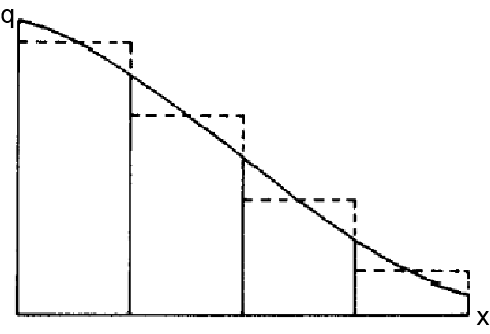
\includegraphics[width=5cm]{ppm_interpolate.png}
  \caption{The image of interpolation function in The piecewise parobolic method (PPM) scheme. The interpolation function is in the solid line, the grid mean value is in the dot line.}
  \label{f1}
\end{figure}

In PPM scheme, the distribution is determined as follows.
\begin{equation}
\begin{split}
\label{a4}
  q(x)=q_{L,i}+\xi (\Delta q_{i}+q_{6,i}(1-\xi))\\
  \xi=\frac{x-x_{i-\frac{1}{2}}}{\Delta x_{i}},  x_{i-\frac{1}{2}}\leq x \leq x_{i+\frac{1}{2}}
  \end{split}
\end{equation}
Here, $q_{L,i}$ is defined as $\lim_{x \to x_{i+\frac{1}{2}}}=q_{L,i}$.
$q_{R,i}$ is defined as $\lim_{x \to x_{i+\frac{1}{2}}}=q_{R,i}$ as well.
In PPM scheme, $q$ is continuous at boundary $i+\frac{1}{2}$, therefore $q_{L,i+1}=q_{R,i}=q_{i+\frac{1}{2}}$ is hold.
In addition,
\begin{equation}
  \Delta q_{i}=q_{R,i}-q_{L,i},\qquad q_{6,i}=6(q_{i}-\frac{1}{2}(q_{L,i})+q_{R,i})
\end{equation}


For calculationg $q_{i+\frac{1}{2}}$ by interpolation, a finite integration of $q$ given as follows is introduced.
\begin{equation}
  A(x)= \int^{x} q(x') dx'
\end{equation}
At boundary of grid,
\begin{equation}
A(x_{i+\frac{1}{2}})=A_{i+\frac{1}{2}}=\sum_{k\leq i}q_{k}\Delta x_{k}
\end{equation}
$q_{i+\frac{1}{2}}$ is calculated by discretization of $q_{i+\frac{1}{2}}=dA/dx |_{x_{i+\frac{1}{2}}}$ by using $(A_{j+k+\frac{1}{2}},x_{j+k+\frac{1}{2}})$, $k=0,\pm 1, \pm 2$.
Specifically, $q_{i+\frac{1}{2}}$ is calculated as follows.
\begin{equation}
  \label{a3}
  \begin{split}
    q_{i+\frac{1}{2}}=&q_{i}+\Delta x_{i} \frac{q_{i+1}-q_{i}}{\Delta x_{i+1}+\Delta x_{i}}+\frac{1}{\sum_{k=i-1}^{i+2}\Delta x_{k}}\\
    &\times \Bigl[\frac{2\Delta x_{i}\Delta x_{i+1}}{\Delta x_{i+1}+\Delta x_{i}}(\frac{\Delta x_{i}+\Delta x_{i-1}}{\Delta x_{i+1}+2\Delta x_{i}}-\frac{\Delta x_{i+2}+\Delta x_{i+1}}{2\Delta x_{i+1}+\Delta x_{i}})(q_{i+1}-q_{i})\\
     & -\Delta x_{i}\frac{\Delta x_{i}+\Delta x_{i-1}}{\Delta x_{i+1}+2\Delta x_{i}} \delta q_{i+1}+\Delta x_{i+1} \frac{\Delta x_{i+2}+\Delta x_{i+1}}{2\Delta x_{i+1}+\Delta x_{i}} \delta q_{i}\Bigr]
  \end{split}
\end{equation}
In case the grid width is equal in all grids, Eq.(\ref{a3}) can be simply rewritten as
\begin{equation}
  q_{i+\frac{1}{2}}=\frac{1}{2}(q_{i-1}+q{i})-\frac{1}{6}(\delta q_{i}-\delta q_{i-1})
\end{equation}
Here, $\delta q_{i}$ is given as
\begin{equation}
  \delta q_{i}=\frac{\Delta x_{i}}{\Delta x_{i-1}+\Delta x_{i}+\Delta x_{i+1}}\biggl[\frac{2\Delta x_{i-1}+\Delta x_{i}}{\Delta x_{i+1}+\Delta x_{i}}(q_{i+1}-q_{i})+\frac{\Delta x_{i}+2\Delta x_{i+1}}{\Delta x_{i-1}+\Delta x_{i}}(q_{i}-q_{i-1})\biggr]
\end{equation}

However, in this case, the interpolation function may have extremes in the grid and may not satisfy monotonicity.
In order to avoid such a situation, $q_{i+\frac{1}{2}}$ should be between $q_{i}$ as $q_{i+1}$, and $\delta q_{i}$ is modified as follows for that.
\begin{equation}
  \begin{aligned}
    \delta_{m} q_{i} & =\min(|\delta
    q_{i}|,2|q_{i}-q_{i-1}|,|q_{i+1}-q_{i}|) && \qquad \text{if$\quad(q_{i+1}-q_{i})(q_{i}-q_{i-1}) >0$}, \\
    & =0 && \qquad \text{otherwise}
  \end{aligned}
\end{equation}
This $\delta q_{i}$ is used in Eq.(\ref{a3}) to calculate $q_{i+\frac{1}{2}}$.

When $q(x)$ is interpolated as Eq.(\ref{a4}), by using Courant number defined as
\begin{equation}
  C=\frac{u_{i+\frac{1}{2}}\Delta t}{\Delta x_{i+1}}
\end{equation}
flux $F^{x}_{i+\frac{1}{2}}$ is wriiten as follows.
\begin{equation}
  F^{x}_{i+\frac{1}{2}}=\begin{cases}u_{i+\frac{1}{2}}[q_{R,i}-\frac{C}{2}(\Delta q_{i}-(1-\frac{2}{3}C)q_{6,i})] & (u_{i+\frac{1}{2}}\ge0)\\
  u_{i+\frac{1}{2}}[q_{L,i+1}+\frac{C}{2}(\Delta q_{i+1}+(1-\frac{2}{3}C)q_{6,i+1})] & (u_{i+\frac{1}{2}}\leq0)
  \end{cases}
\end{equation}
\subsubsubsection{Devices for Taking Long Time Steps}
The above argument is stable only if $C<1$
When the grid method is adapted to spherical coordinate, $\Delta x$ is very small in polar region.
Therefore, we have to take very small $\Delta t$ to satisfy CFL condition.
The special treatment when $C>1$ for taking larger $\Delta t$ are described below.
Although this method is used for any grid widths, in this subsection we assume that $\Delta x$ does not depend on $i$ for simplicity.

Courant number can be divided into a integral fraction and a decimal fraction.
\begin{equation}
  C=I_{C}+\hat{C},\quad I_{C}: \text{an integer fraction},\quad -0.5\le \hat{C} \le 0.5
\end{equation}
When $I_{C}>0$
\begin{equation}
  F^{x}_{i-\frac{1}{2}}=\hat{F^{x}_{i-I_{C}+\frac{1}{2}}}+\sum^{i}_{i'=i+1-I_{C}} q_{i'} \frac{\Delta x_{i}}{\Delta t}
\end{equation}
When $I_{C}<0$
\begin{equation}
  F^{x}_{i-\frac{1}{2}}=\hat{F^{x}_{i+|I_{C}|+\frac{1}{2}}}+\sum^{i+|I_{C}|}_{i'=i+1} q_{i'} \frac{\Delta x_{i}}{\Delta t}
\end{equation}
Where $\hat{F^{x}_{i-I_{C}+\frac{1}{2}}}$ is the flux of point $(i-I_{C}+\frac{1}{2})$ calculated by using $\hat{C}$.

As indicated above, in the case the fluid moves in multiple grids during $\Delta t$, we can avoid instability of numerical calculation by evaluating the flux using the quantity $q_{i'}$ corresponding to each grids passed.
In actual, these argument is applied only to zonal flux, which can break CFL condition.

\subsubsubsection{The Treatment of Cross Terms}
In the case velocity of the fluid is not only in the x-direction or y-direction, only adding the flux contributions in the x- and y-directions together underestimate the effect of diagonal advection.
To take these cross term into considering, the following procedure is taken.
Here, we discuss this in two-dimensional space, not in one-dimensional.

When calculating x-direction flux $F^{x}_{i+\frac{1}{2},j}$, upstream value of $q$ in y-direction is used as value of $q$.
That is expressed by the following equation.
  \begin{equation}
    q^{y}_{i,j}=\frac{1}{2} {q(x_{i},y_{i}-v_{i,j}\Delta t)+q_{i,j}}
  \end{equation}
Here, $q(x_{i},y_{i}-v_{i,j}\Delta t)$ is calculated by linear interpolation of the two nearest grid points.
In the same way, when calculating y-direction flux $F^{x}_{i+\frac{1}{2},j}$,
  \begin{equation}
    q^{x}_{i,j}=\frac{1}{2} {q(x_{i}-u_{i,j}\Delta t,y_{i})+q_{i,j}}
  \end{equation}
  is used as $q$.

  In the case of three dimensional tracer advection, this procedure is conducted in two dimension.

  \subsubsection{Actual Tracer Advection Scheme in MIROC6}
  In this subsection, the procedure implemented in MIROC6 of the tracer advection scheme is described.
  Although MIROC6 adopts $\sigma$-$p$ hybrid coordinate as vertical coordinate, the tracer advection scheme is largely based on $\sigma$ coordinate because previous version of MIROC adopted $\sigma$ coordinate.
  Therefore, firstly the procedure under $\sigma$ coordinate system is described.
  After this, the changes in the hybrid coordinate system from the $\sigma$ coordinate system is described.
  \subsubsubsection{$\sigma$-Coordinate}
The transport equation in $\sigma$ coordinate on the sphere is expressed as
\begin{eqnarray}
  \label{b1}
  \frac{\partial P^{S} q}{\partial t} &=& - \frac{1}{a \cos \varphi} \frac{\partial}{\partial \lambda}(P^{S} uq)- \frac{1}{a \cos \varphi} \frac{\partial}{\partial \varphi}(P^{S} vq \cos \varphi)- \frac{\partial}{\partial \sigma} (P^{S} \dot{\sigma} q)\\
  &=& \frac{1}{a \cos \varphi} \frac{\partial}{\partial \lambda}(F^{\lambda})- \frac{1}{a \cos \varphi} \frac{\partial}{\partial \varphi}(F^{\varphi})- \frac{\partial}{\partial \sigma} (F^{\sigma})
\end{eqnarray}
$P^{S}$ is surface pressure, $q$ is quantity of tracers.
Continuity equation is given by considering the case of $q=1$.
\begin{equation}
  \frac{\partial P^{S}}{\partial t} = - \frac{1}{a \cos \varphi} \frac{\partial}{\partial \lambda}(P^{S}u)- \frac{1}{a \cos \varphi} \frac{\partial}{\partial \varphi}(P^{S}v \cos \varphi)- \frac{\partial}{\partial \sigma} (P^{S} \dot{\sigma})
\end{equation}
Assuming that grid is equally spaced in zonal direction, the transport equation is discretized as follows.
\begin{equation}
\label{a1}
  \frac{\partial P^{S}_{,i,j,k} q_{i,j,k}}{\partial t}=\frac{1}{\Delta D_{j,k}}[(G^{\lambda}_{i-\frac{1}{2},j,k}-G^{\lambda}_{i+\frac{1}{2},j,k})+(G^{\varphi}_{i,j-\frac{1}{2},k}-G^{\varphi}_{i,j+\frac{1}{2},k}))+(G^{\sigma}_{i,j,k-\frac{1}{2}}-G^{\sigma}_{i,j,k+\frac{1}{2}})]
\end{equation}
Here,
\begin{equation}
  G^{\lambda}_{i-\frac{1}{2},j,k}=F^{\lambda}_{i-\frac{1}{2},j,k} \Delta y_{j} \Delta \sigma_{k}=(P^{S}uq)_{i-\frac{1}{2},j,k} \Delta y_{j} \Delta \sigma_{k}
\end{equation}
\begin{equation}
  G^{\varphi}_{i,j-\frac{1}{2},k}=F^{\varphi}_{i,j-\frac{1}{2},k} \Delta x_{j-\frac{1}{2}} \Delta \sigma_{k}=(P^{s}vq)_{i,j-\frac{1}{2},k} \Delta x_{j-\frac{1}{2}} \Delta \sigma_{k}
\end{equation}
\begin{equation}
  G^{\sigma}_{i,j,k-\frac{1}{2}}=F^{\eta}_{i,j,k-\frac{1}{2}} \Delta x_{j} \Delta y_{j}=(P^{S} \dot{\sigma} q)_{i,j,k-\frac{1}{2}} \Delta x_{j} \Delta y_{j}
\end{equation}
And
\begin{equation}
  \Delta D_{j,k}=a \cos \varphi_{j} \Delta \lambda \Delta \varphi_{j} \Delta \sigma_{k},\quad \Delta x_{j}=a \cos \varphi_{j} \Delta \lambda,\quad \Delta y_{j}=a \Delta \varphi_{j}
\end{equation}
This flux form equation ensure the conservation.

For the calculation of the time-averaged mass flux across the cell boundary, the winds and the tracer distributions are staggered in the Arakawa C-grid (Mesinger and Arakawa 1976). The horizontal winds at the cell boundary, $u_{i-\frac{1}{2},j,k}, v_{i-\frac{1}{2},j,k}$, are reconstructed by using the mass convergence field in the spectral model and the discretized continuity eqution:
\begin{equation}
  \frac{\partial P^{S}_{i,j,k} }{\partial t}=\frac{1}{\Delta D_{j,k}}[(V^{\lambda}_{i-\frac{1}{2},j,k}-V^{\lambda}_{i+\frac{1}{2},j,k})+(V^{\varphi}_{i,j-\frac{1}{2},k}-V^{\varphi}_{i,j+\frac{1}{2},k}))+(V^{\sigma}_{i,j,k-\frac{1}{2}}-V^{\sigma}_{i,j,k+\frac{1}{2}})]
\end{equation}
Here, $V^{\lambda}_{i-\frac{1}{2},j,k}, V^{\varphi}_{i,j-\frac{1}{2},k}, V^{\sigma}_{i,j,k-\frac{1}{2}}$ denote zonal, meridional, and vertical mass-weighted wind at the cell boundary, rspectively. That is,
\begin{equation}
  V^{\lambda}_{i-\frac{1}{2},j,k}=(P^{S}u)_{i-\frac{1}{2},j,k} \Delta y_{j} \Delta \sigma_{k}
\end{equation}
\begin{equation}
  V^{\varphi}_{i,j-\frac{1}{2},k}=(P^{S}v)_{i,j-\frac{1}{2},k} \Delta x_{j-\frac{1}{2}} \Delta \eta_{k}
\end{equation}
\begin{equation}
  V^{\sigma}_{i,j,k-\frac{1}{2}}=(P^{S}\dot{\sigma})_{i,j,k-\frac{1}{2}} \Delta x_{j} \Delta y_{j}
\end{equation}
$\Delta D_{j,k}$ denotes the cell volume, and $\Delta x_{j}, \Delta y_{j}$, and $\Delta \sigma_{k}$ denote zonal, meridional and vertical width of the cell, respectively. That is $\Delta D_{j,k}=a \cos \varphi_{j}\Delta \lambda \Delta \varphi_{j} \Delta \sigma$, $\Delta x_{j}=a \cos \varphi_{j} \Delta \lambda$ and $\Delta y_{j}=a \Delta \varphi_{j}$.

The following are the procedure for the calculation of tracer advection in the staggering-grided horizontal and vertical wind fields:
\begin{enumerate}
\item Surface pressure $P^{S}(t+\Delta t)$ and horizontal wind $\bf{v}(t+\Delta t)$ are predicted in the spectral model.
\item The horizontal component of mass flux divergence at time step $t$ is calculated by using spherical harmonics. The mass fluxes at time step $t$ are reconstructed from the values at $t+\Delta t$ and $t-\Delta t$ because MIROC applies semi-implicit scheme for the time-integration of surface pressure. Zonal and meridional component of mass flux divergence are:
  \begin{equation}
    C^{x}=-\frac{1}{a \cos \varphi}\frac{\partial}{\partial \lambda}(P^{s}u),\quad C^{y}=-\frac{1}{a \cos \varphi}\frac{\partial}{\partial \lambda}(P^{s}v \cos \varphi)
  \end{equation}
\item By using $C_{x}$ and $C_{y}$, $V^{\lambda}, V^{\varphi}, V^{\sigma}$ are calculated as follows.
  \begin{equation}
    V^{\lambda}_{i-\frac{1}{2},j,k}-V^{\lambda}_{i+\frac{1}{2},j,k}=C^{x}_{i,j,k}\Delta D_{j,k}, \quad V^{\lambda}_{i,j-\frac{1}{2},k}-V^{\lambda}_{i,j+\frac{1}{2},k}=C^{y}_{i,j,k}\Delta D_{j,k}
  \end{equation}
  The boundry conditions are $V^{\varphi}=0$ at the North Pole and South Pole, $\sigma=1$ at surface and $V^{\sigma}=0$ at $\sigma=0$.
The condition for $V^{\lambda}=0$ is:
  \begin{equation}
    \sum_{i}V^{\lambda}_{i-\frac{1}{2},j,k}=\sum_{i}P^{S}_{i,j,k}u_{i,j,k}\Delta y_{j}\Delta \sigma_{k}
  \end{equation}
  That means zonal mean of zonal mass transport is equal to that in the spectral model grid.
  Here, the following equation must be satisfied for boundary condition $V^{\varphi}=0$ at the North Pole and the South Pole.
  \begin{equation}
    \sum_{j}C^{y}_{i,j,k}\Delta D_{j,k}=0
  \end{equation}
  However, this is not always satisfied (On the other hand, $\sum_{i} \sum_{j}C^{y}_{i,j,k}\Delta D_{j,k}=0$ is valid within numerical error.).

  In order to satisfy the boundary condition, the following correction is made.
  \begin{equation}
    C^{y}_{i,j,k}\leftarrow C^{y}_{i,j,k}-\delta C, \quad C^{y}_{i,j,k}\leftarrow C^{x}_{i,j,k}+\delta C
  \end{equation}
  Here, $\delta C=\sum_{j}C^{y}_{i,j,k}\Delta D_{j,k}/\sum_{j}\Delta D_{j,k}$.
  Vertical velocity $V^{\eta}$ is obtained by using
  \begin{equation}
    \label{a2}
    \frac{\partial P^{S}_{i,j,k}}{\partial t}\sum_{k}\Delta D_{j,k}=\sum_{k}(C^{x}_{i,j,k}+C^{y}_{i,j,k})
  \end{equation}
  (The contents so far are in [TRACEG] of dtrcr.F.  The rest of the content is in [GTRACE] of dtrcr.F.)
\item $G^{\lambda}, G^{\varphi}, G^{\sigma}$ are calculated by PPM scheme from $V^{\lambda}, V^{\varphi}, V^{\sigma}$.

\item $P^{s}_{i,j,k}q_{i,j,k}$ at time step $t+\Delta t$ is calulated by integration of Eq.(\ref{a1}) by leap frog method from $G^{\lambda}, G^{\varphi}, G^{\sigma}$.

\item $q_{t+\Delta t}$ is calculated by dividing $(P^{s}q)_{t+\Delta t}$ by $P^{s}_{t+\Delta t}$.
  There is small quantity of difference between $P^{s}_{t+\Delta t}$ from Eq. (\ref{a2}) and $P^{s}_{t+\Delta t}$ in the spectral model, because semi-implicit time integration scheme is applied.
  $P^{s}_{t+\Delta t}$ from Eq. (\ref{a2}) is applied at present for the consistency of mass advection. Mass Conservation is not strictly satisfied because of the discrepancy between the surface pressure in the spectral model and from $P^{s}_{t+\Delta t}$ Eq. (\ref{a2}).
\end{enumerate}

\subsubsubsection{$\sigma$-$p$ Hybrid Coordinate}
The transport equation in $\eta$ coordinate ($\sigma-p$ hybrid coordinate) on the sphere is:
\begin{eqnarray}                                                             \frac{\partial mq}{\partial t} &=& - \frac{1}{a \cos \varphi} \frac{\partial}{\partial \lambda}(muq)- \frac{1}{a \cos \varphi} \frac{\partial}{\partial \varphi}(mvq \cos \varphi)- \frac{\partial}{\partial \eta} (m \dot{\eta} q)\\                                                                         &=& \frac{1}{a \cos \varphi} \frac{\partial}{\partial \lambda}(F^{\lambda})- \frac{1}{a \cos \varphi} \frac{\partial}{\partial \varphi}(F^{\varphi})-\frac{\partial}{\partial \eta} (F^{\eta})
\end{eqnarray}
Here,$m$ corresponds to the density of the coordinate and is defined as $m=\frac{\partial p}{\partial \eta}$.
if you look at Eq. (\ref{b1}), you can find that difference of $\sigma$ coordinate and $\eta$ coordinate is only that $P^{S}$ replaces $m$.
The actual tracer advection in $\eta$ coordinate is mostly the same as $\sigma$ coordinate.

In the scheme in $\eta$ coordinate, the following variables are calculated in the same way as the way $G^{\lambda}, G^{\varphi}, G^{\eta}$ is calculated in $\sigma$ coordinate, except $\Delta \sigma$ replaces with $\Delta \eta$ and $\dot{\sigma}$ replaces with $\dot{\eta}$.
\begin{equation}
  G^{\prime \lambda}_{i-\frac{1}{2},j,k}=(P^{S}uq)_{i-\frac{1}{2},j,k} \Delta y_{j} \Delta \eta_{k},\quad G^{\prime \varphi}_{i,j-\frac{1}{2},k}=(P^{S}vq)_{i,j-\frac{1}{2},k} \Delta x_{j-\frac{1}{2}} \Delta \eta_{k},\quad G^{\prime \eta}_{i,j,k-\frac{1}{2}}=(P^{S} \dot{\eta} q)_{i,j,k-\frac{1}{2}} \Delta x_{j} \Delta y_{j}
\end{equation}
In the time integration step, multiplying $G\prime$ by $m/P^{S}$, $G^{\lambda}, G^{\varphi}, G^{\eta}$ is calculated.
After that, $mq$ at time step $t+\Delta t$ is calculated by leap-frog method as well as $\sigma$ coordinate.

In actual source code, conbining to dividing by $m$ to calculate $q$ at time step $t+\Delta t$, $q$ at point $(i,j,k)$ in time step $t+\Delta t$ is calculated as follows.
\begin{equation}
  \begin{split}
        q^{t+\Delta t}=&\frac{\Delta A_{k}+\Delta B_{k} P^{S,t-\Delta t}_{i,j,k}}{\Delta A_{k}+\Delta B_{k} P^{S,t+\Delta t}_{i,j,k}}q^{t-\Delta t}_{i,j,k}+\frac{2\Delta t}{\Delta D}\\
    &\times [(G^{\prime \lambda,t}_{i-\frac{1}{2},j,k}-G^{\prime \lambda,t}_{i+\frac{1}{2},j,k})+(G^{\prime \varphi,t}_{i,j-\frac{1}{2},k}-G^{\prime \varphi,t}_{i,j+\frac{1}{2},k}))+(G^{\prime \eta,t}_{i,j,k-\frac{1}{2}}-G^{\prime \eta,t}_{i,j,k+\frac{1}{2}})]\\
    &\times \frac{\Delta A_{k}+\Delta B_{k} P^{S,t}_{i,j,k}}{P^{S,t}_{i,j,k}}\frac{1}{\Delta A_{k}+\Delta B_{k} P^{S,t+\Delta t}_{i,j,k}}
  \end{split}
\end{equation}
Here,$A,B$ is the coefficients for $\eta$ coordinate, $\eta_{k+\frac{1}{2}}=A_{k+\frac{1}{2}}/p_{0}+B_{k+\frac{1}{2}}$ and $\Delta A_{k}=A_{k-\frac{1}{2}}-A_{k+\frac{1}{2}},\quad \Delta B_{k}=B_{k-\frac{1}{2}}-B_{k+\frac{1}{2}}$.
And $\Delta A_{k}+\Delta B_{k} P^{S}_{i,j,k}=\Delta p_{i,j,k}$(More details in the section of the vertical discretization).

\subsubsubsection{The Mass Fluxes into/out of Polar Caps}
The mass fluxes into/out of polar caps are calculated by using the semi–Lagrangian scheme in the polar stereo projection (cf. Fig.\ref{f2}).
The horizontal average at the highest latitude band is assumed to be preserved before/after flux calculation for the mass conservation. The sequence of calculation is:
\begin{enumerate}
\item Zonal average of $P^{S}q$ at time step $t$ is calculated at the highest latitude band $(j=j_{N},j_{S})$, and is assumed to equal $P^{S}q$ at the pole.
\item Horizontal wind at the highest latitude bands is projected into the orthogonal coordinate system centering around the pole, and $q$ at time step $t + \Delta t$ is estimated by using the value at the “departure point”.
\item Zonal anerage of $P^{S}q$ at time step $t+\Delta t$ is fixed to that at $t$.
\end{enumerate}

\begin{figure}
  \centering
  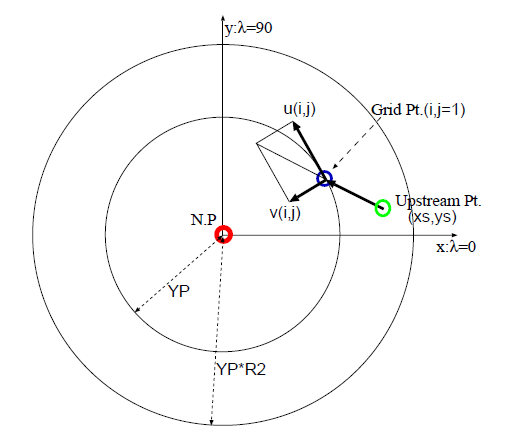
\includegraphics[width=5cm]{polar_tracer_advection.png}
  \caption{Conceptual figure for the flux on pole-most grids.}
  \label{f2}
\end{figure}
%\end{document}

	\hypertarget{summary-of-the-dynamical-core}{%
\subsection{Summary of the dynamical
core}\label{summary-of-the-dynamical-core}}

In this section, we enumerate the calculations performed in the
dynamical core, although they overlap with the previous descriptions.

\hypertarget{conversion-of-horizontal-wind-to-vorticity-and-divergence}{%
\subsubsection{Conversion of Horizontal Wind to Vorticity and
Divergence}\label{conversion-of-horizontal-wind-to-vorticity-and-divergence}}

Obtain grid point values of vorticity and divergence from the grid point
values of \(u_{ij}, v_{ij}\) for horizontal wind. First, we obtain the
vorticity and divergence in spectral space, \(\zeta_n^m, D_n^m\),

\begin{eqnarray}
\zeta_n^m  =  \frac{1}{I} \sum_{i=1}^{I} \sum_{j=1}^{J}  
                  \mathrm{i}m v_{ij} \cos\varphi_j {Y_n^{m*}}_{ij}
                \frac{w_j}{a(1-\mu_j^{2})}
           +    \frac{1}{I} \sum_{i=1}^{I} \sum_{j=1}^{J}  
                     u_{ij} \cos\varphi_j (1-\mu_j^2)
                  \frac{\partial }{\partial \mu} {Y_n^{m*}}_{ij}
                 \frac{w_j}{a(1-\mu_j^{2})} \; ,
\end{eqnarray}

\begin{eqnarray}
    D_n^m  =  \frac{1}{I} \sum_{i=1}^{I} \sum_{j=1}^{J}  
                  \mathrm{i}m u_{ij} \cos\varphi_j {Y_n^{m*}}_{ij}
                \frac{w_j}{a(1-\mu_j^{2})}
           -    \frac{1}{I} \sum_{i=1}^{I} \sum_{j=1}^{J}  
                  v_{ij} \cos\varphi_j  (1-\mu_j^2)
                  \frac{\partial }{\partial \mu} {Y_n^{m*}}_{ij}
                 \frac{w_j}{a(1-\mu_j^{2})} ; .
\end{eqnarray}

The grid point value is calculated by

\begin{eqnarray}
  \zeta_{ij}
   =  {\mathcal R}{\mathbf{e}} \sum_{m=-N}^{N} \sum_{n=|m|}^{N}
      \zeta_n^m  {Y_n^m}_{ij} \; ,
\end{eqnarray}

and so on.

Corresponding file \& subroutines:
\texttt{{[}G2Wpush,\ G2Wtrans,\ G2Wshift,\ W2Gpush,\ W2Gtrans,\ W2Gshift\ (xdsphe.F){]}}

\hypertarget{calculating-a-virtual-temperature}{%
\subsubsection{Calculating a virtual
temperature}\label{calculating-a-virtual-temperature}}

virtual Temperature \(T_v\) is ,

\begin{eqnarray}
  T_v = T ( 1 + \epsilon_v q - l ) \; ,
\end{eqnarray}

However, it is \(\epsilon_v = R_v/R - 1\) and \(R_v\) is the gas
constant for water vapor (461 Jkg\(^{-1}\)K\(^{-1}\)) and \(R\) is the
gas constant for air (287.04 Jkg\(^{-1}\)K\(^{-1}\)).

Corresponding file \& subroutines: \texttt{{[}VIRTMD\ (dvtmp.F){]}}
\#\#\# Calculating the pressure gradient term

The pressure gradient term \(\nabla \pi = \frac{1}{p_S} \nabla p_S\) is
first used to define the \(\pi_n^m\)

\begin{eqnarray}
  \pi_n^m  =  \frac{1}{I} \sum_{i=1}^{I} \sum_{j=1}^{J}  
               (\ln {p_S})_{ij} {Y_n^{m *}}_{ij}  w_j \; ,
\end{eqnarray}

to a spectral representation and then ,

\begin{eqnarray}
   \frac{1}{a \cos \varphi}
   \left( \frac{\partial \pi}{\partial \lambda} \right)_{ij}
     =
   \frac{1}{a \cos \varphi}
        {\mathcal R}{\mathbf{e}} \sum_{m=-N}^{N} \sum_{n=|m|}^{N}
       \mathrm{i}m \tilde{X}_n^m {Y_n^m}_{ij}  \; ,
\end{eqnarray}

\begin{eqnarray}
   \frac{1}{a}
   \left( \frac{\partial \pi}{\partial \varphi} \right)_{ij}
     =  
   \frac{1}{a \cos \varphi}
       {\mathcal R}{\mathbf{e}} \sum_{m=-N}^{N} \sum_{n=|m|}^{N}
       \pi_n^m
       ( 1-\mu^{2} ) \frac{\partial }{\partial \mu} {Y_n^m}_{ij}  \; .
\end{eqnarray}

Corresponding file \& subroutine: \texttt{{[}PSDOT\ (dgdyn.F){]}}

\hypertarget{diagnosis-of-vertical-flow}{%
\subsubsection{Diagnosis of vertical
flow}\label{diagnosis-of-vertical-flow}}

Pressure change term, and lead DC,

\begin{eqnarray}
  \frac{\partial \pi}{\partial t}
   = - \sum_{k=1}^{K} \left\{ D_k \Delta\sigma_k + ({\mathbf{v}}_k \cdot \nabla \pi)\Delta B_k \right\}
\end{eqnarray}

\begin{eqnarray}
  \frac{(m\dot{\eta})_{k-1/2}}{p_s}
   = - B_{k-1/2} \frac{\partial \pi}{\partial t}
    - \sum_{l=k}^{K}\left\{ D_l \Delta\sigma_l + ({\mathbf{v}}_l \cdot \nabla \pi)\Delta B_l \right\}
\end{eqnarray}

and its non-gravity components.

\begin{eqnarray}
  \left( \frac{\partial \pi}{\partial t} \right)^{NG}
   =   - \sum_{k=1}^{K} {\mathbf{v}}_{k} \cdot \nabla \pi  
       \Delta B_{k}
\end{eqnarray}

\begin{eqnarray}
  \frac{(m\dot{\eta})^{NG}_{k-1/2}}{p_s}
   = - B_{k-1/2} \left( \frac{\partial \pi}{\partial t} \right)^{NG}
    - \sum_{l=k}^{K} {\mathbf{v}}_{l} \cdot \nabla \pi
       \Delta B_{l}
\end{eqnarray}

Corresponding file and subroutine: \texttt{{[}PSDOT\ (dgdyn.F){]}}

\hypertarget{tendency-terms-due-to-advection}{%
\subsubsection{Tendency terms due to
advection}\label{tendency-terms-due-to-advection}}

Momentum advection term:

\begin{eqnarray}
  (A_u)_k
    =  ( \zeta_k + f ) v_k
             - \left[ \frac{(m\dot{\eta})_{k-1/2}}{p_s} \frac{u_{k-1} - u_k}{\Delta\sigma_{k-1}+\Delta\sigma_k}
               + \frac{(m\dot{\eta})_{k+1/2}}{p_s} \frac{u_k   - u_{k+1}}{\Delta\sigma_{k}+\Delta\sigma_{k+1}} \right]
\end{eqnarray} \begin{eqnarray}
           - \frac{1}{a\cos\varphi} \frac{\partial \pi}{\partial \lambda}(C_p T_{v,k}\hat{\kappa}-R\bar{T})
             + {\mathcal F}_x
\end{eqnarray}

\begin{eqnarray}
  (A_v)_k
    =  - ( \zeta_k + f ) u_k
             - \left[ \frac{(m\dot{\eta})_{k-1/2}}{p_s} \frac{v_{k-1} - v_k}{\Delta\sigma_{k-1}+\Delta\sigma_k}
               + \frac{(m\dot{\eta})_{k+1/2}}{p_s} \frac{v_k   - v_{k+1}}{\Delta\sigma_{k}+\Delta\sigma_{k+1}} \right]
\end{eqnarray} \begin{eqnarray}
           - \frac{1}{a} \frac{\partial \pi}{\partial \varphi}(C_p T_{v,k}\hat{\kappa}-R\bar{T})
             + {\mathcal F}_y
\end{eqnarray}

Temperature advection term:

\begin{eqnarray}
 (u T')_k  = u_k (T_k - \bar{T} )
\end{eqnarray}

\begin{eqnarray}
 (v T')_k  = v_k (T_k - \bar{T} )
\end{eqnarray}

\begin{eqnarray}
   H_k =  T_k' D_k
          - \left[ \frac{(m\dot{\eta})_{k-1/2}}{p_s} \frac{\hat{T}_{k-1/2} - T_k}{\Delta \sigma_l}
               + \frac{(m\dot{\eta})_{k+1/2}}{p_s} \frac{T_k - \hat{T}_{k+1/2}}{\Delta \sigma_l} \right]
\end{eqnarray} \begin{eqnarray}
        + \hat{\kappa}_k {\mathbf{v}}_k \cdot \nabla \pi T_{v,k}
\end{eqnarray} \begin{eqnarray}
        - \alpha_k \sum_{l=k}^{K}
                           (D_l \Delta \sigma_l + ({\mathbf{v}}_l \cdot \nabla \pi)\Delta B_l)
                            \frac{T_{v,k}}{\Delta \sigma_k}
\end{eqnarray} \begin{eqnarray}
        - \beta_k \sum_{l=k+1}^{K}
                           (D_l \Delta \sigma_l + ({\mathbf{v}}_l \cdot \nabla \pi)\Delta B_l)
                            \frac{T_{v,k}}{\Delta \sigma_k}
\end{eqnarray}

Water vapor advection term:

\begin{eqnarray}
 (u q)_k  = u_k q_k
\end{eqnarray}

\begin{eqnarray}
 (v q)_k  = v_k q_k
\end{eqnarray}

\begin{eqnarray}
R_k  =  q_k D_k
       - \frac{1}{2}
             \left[   \frac{(m\dot{\eta})_{k-1/2}}{p_s} \frac{q_{k-1} - q_k}{\Delta\sigma_k}
               + \frac{(m\dot{\eta})_{k+1/2}}{p_s} \frac{q_k   - q_{k+1}}{\Delta\sigma_k} \right]
\end{eqnarray}

Corresponding file \& subroutine
\texttt{{[}GRTADV,\ GRUADV\ (dgdyn.F){]}}

\hypertarget{transformation-of-prognostic-variables-to-spectral-space}{%
\subsubsection{Transformation of prognostic variables to spectral
space}\label{transformation-of-prognostic-variables-to-spectral-space}}

\begin{enumerate}
\def\labelenumi{(\arabic{enumi})}
\setcounter{enumi}{121}
\tightlist
\item
  and (123).
\end{enumerate}

Transform \(u_{ij}^{t-\Delta t}, v_{ij}^{t-\Delta t}\) to a spectral
representation of vorticity and divergence \(\zeta_n^m, D_n^m\).
Furthermore, transforming the temperature \(T^{t-\Delta t}\), specific
humidity \(q^{t-\Delta t}\), and \(\pi = \ln p_S^{t-\Delta t}\) to

\begin{eqnarray}
  X_n^m  =  \frac{1}{I} \sum_{i=1}^{I} \sum_{j=1}^{J}  
               X_{ij} {Y_n^{m *}}_{ij}  w_j \; ,
\end{eqnarray}

to a spectral representation.

Corresponding file \& subroutine:
\texttt{{[}G2Wpush,\ G2Wtrans,\ G2Wshift\ (xdsphe.F){]}}

\hypertarget{transformation-of-tendency-terms-to-spectral-space}{%
\subsubsection{Transformation of tendency terms to spectral
space}\label{transformation-of-tendency-terms-to-spectral-space}}

Tendency Term of Vorticity

\begin{eqnarray}
  \frac{\partial{\zeta_n^m}}{\partial {t}}
    =  \frac{1}{I} \sum_{i=1}^{I} \sum_{j=1}^{J}  
    \mathrm{i}m (A_v)_{ij} \cos \varphi_j
    {Y_n^{m *}}_{ij}
    \frac{w_j}{a(1-\mu_j^{2})}
\\
  +\frac{1}{I} \sum_{i=1}^{I} \sum_{j=1}^{J}  
    (A_u)_{ij} \cos \varphi_j
    (1-\mu_j^2)
    \frac{\partial }{\partial \mu} {Y_n^{m *}}_{ij}
    \frac{w_j}{a(1-\mu_j^{2})}
\end{eqnarray}

The non-gravity wave component of the tendency term of the divergence

\begin{eqnarray}
  \left( \frac{\partial{D_n^m}}{\partial {t}} \right)^{NG}
   =  \frac{1}{I} \sum_{i=1}^{I} \sum_{j=1}^{J}  
          \mathrm{i}m (A_u)_{ij} \cos \varphi_j
          {Y_n^{m *}}_{ij}
         \frac{w_j}{a(1-\mu_j^{2})}
          \\
   -\frac{1}{I} \sum_{i=1}^{I} \sum_{j=1}^{J}  
          (A_v)_{ij} \cos \varphi_j
          (1-\mu_j^2)
          \frac{\partial }{\partial \mu} {Y_n^{m *}}_{ij}
          \frac{w_j}{a(1-\mu_j^{2})}
          \\
   -\frac{n(n+1)}{a^{2}}
         \frac{1}{I} \sum_{i=1}^{I} \sum_{j=1}^{J}  
          \hat{E}_{ij}  {Y_n^{m *}}_{ij} w_j
          \\
\end{eqnarray}

The non-gravity wave component of the tendency term of temperature

\begin{eqnarray}
  \left( \frac{\partial{T_n^m}}{\partial {t}} \right)^{NG}
   =  - \frac{1}{I} \sum_{i=1}^{I} \sum_{j=1}^{J}  
          \mathrm{i}m (u T')_{ij} \cos \varphi_j
          {Y_n^{m *}}_{ij}
         \frac{w_j}{a(1-\mu_j^{2})}
          \\
     + \frac{1}{I} \sum_{i=1}^{I} \sum_{j=1}^{J}  
          (v T')_{ij} \cos \varphi_j
          (1-\mu_j^2)
          \frac{\partial }{\partial \mu} {Y_n^{m *}}_{ij}
          \frac{w_j}{a(1-\mu_j^{2})}
          \\
     + \frac{1}{I} \sum_{i=1}^{I} \sum_{j=1}^{J}  
          \hat{H}_{ij}
          {Y_n^{m *}}_{ij} w_j
\end{eqnarray}

Tendency term of water vapor

\begin{eqnarray}
  \frac{\partial{q_n^m}}{\partial {t}}
   =  - \frac{1}{I} \sum_{i=1}^{I} \sum_{j=1}^{J}  
          \mathrm{i}m (uq)_{ij} \cos \varphi_j
          {Y_n^{m *}}_{ij}
         \frac{w_j}{a(1-\mu_j^{2})}
          \\
     + \frac{1}{I} \sum_{i=1}^{I} \sum_{j=1}^{J}  
          (vq)_{ij} \cos \varphi_j
          (1-\mu_j^2)
          \frac{\partial }{\partial \mu} {Y_n^{m *}}_{ij}
          \frac{w_j}{a(1-\mu_j^{2})}
          \\
     + \frac{1}{I} \sum_{i=1}^{I} \sum_{j=1}^{J}  
          R_{ij}
          {Y_n^{m *}}_{ij} w_j
\end{eqnarray}

Corresponding file \& subroutines:
\texttt{{[}G2Wpush,\ G2Wtrans,\ G2Wshift\ (xdsphe.F){]}}

\hypertarget{time-integration-in-spectral-space}{%
\subsubsection{Time integration in spectral
space}\label{time-integration-in-spectral-space}}

Equations in matrix form

\begin{eqnarray}
      \left\{ ( 1+2\Delta t {\mathcal D}_H )( 1+2\Delta t {\mathcal D}_M )
           \underline{I}  
      - ( \Delta t )^{2}  ( \underline{W} \ \underline{h}
           + (1+2\Delta t {\mathcal D}_M)
             {\mathbf{G}} {\mathbf{C}}^{T} ) \nabla^{2}_{\sigma}
  \right\}
      \overline{ {\mathbf{D}} }^{t}
       \\
  = ( 1+2\Delta t {\mathcal D}_H )( 1-\Delta t {\mathcal D}_M )
       {\mathbf{D}}^{t-\Delta t}
  +\Delta t
         \left( \frac{\partial {\mathbf{D}}}{\partial t} \right)_{NG}  
  \\
  -\Delta t \nabla^{2}_{\sigma}     
                   \left\{  ( 1+2\Delta t {\mathcal D}_H ) {\mathbf{\Phi}}_{S}
                          + \underline{W}
                            \left[ ( 1-2\Delta t {\mathcal D}_H )
                                    {\mathbf{T}}^{t-\Delta t}
                                  + \Delta t
                                      \left( \frac{\partial {\mathbf{T}}}
                                                  {\partial t}     
                                      \right)_{NG} \right]
                   \right.
  \\
                 \left.  \hspace*{20mm}
                          + ( 1+2\Delta t {\mathcal D}_H ) {\mathbf{G}}
                            \left[ \pi^{t-\Delta t}
                                  + \Delta t
                                     \left( \frac{\partial \pi}
                                                 {\partial t}
                                     \right)_{NG}  \right]
                   \right\} .
\end{eqnarray}

Using LU decomposition, \(\bar{D}\) is obtained by solving for

\begin{eqnarray}
  \frac{\partial {\mathbf{T}}}{\partial t}
      =   \left( \frac{\partial {\mathbf{T}}}
                        {\partial t}       \right)_{NG}  
         - \underline{h} {\mathbf{D}}
\end{eqnarray}

\begin{eqnarray}
  \frac{\partial \pi}{\partial t}
      =   \left( \frac{\partial \pi}
                        {\partial t}       \right)_{NG}  
         - {\mathbf{C}} \cdot {\mathbf{D}}
\end{eqnarray}

Calculate the value of the spectrum in
\(\partial {\mathbf{T}}/\partial t\), \(\partial \pi/\partial t\) and
then calculate the value of the spectrum in \(t+\Delta t\) using

\begin{eqnarray}
  \zeta^{t+\Delta t}  =  \left( \zeta^{t-\Delta t}
                                +   2 \Delta t \frac{\partial{\zeta}}{\partial {t}} \right)
                          ( 1 + 2 \Delta t {\mathcal D}_M )^{-1} \\
  D^{t+\Delta t}  =  2 \bar{D} - D^{t-\Delta t}\\
  T^{t+\Delta t}  =  \left( T^{t-\Delta t}
                                +  2 \Delta t  \frac{\partial{T}}{\partial {t}} \right)
                          ( 1 + 2 \Delta t {\mathcal D}_H )^{-1} \\
  q^{t+\Delta t}  =  \left( q^{t-\Delta t}
                                +  2 \Delta t \frac{\partial{q}}{\partial {t}} \right)
                          ( 1 + 2 \Delta t {\mathcal D}_E )^{-1} \\
\pi^{t+\Delta t}  =  \pi^{t-\Delta t}
                                +  2 \Delta t \frac{\partial{\pi}}{\partial {t}}
\end{eqnarray}

Corresponding file \& subroutine: \texttt{{[}TINTGR\ (dintg.F){]}}

\hypertarget{transformation-of-prognostic-variables-to-grid-point-values}{%
\subsubsection{Transformation of prognostic variables to grid point
Values}\label{transformation-of-prognostic-variables-to-grid-point-values}}

Obtain grid values of horizontal wind speed from the spectral values of
vorticity and divergence (\(\zeta_n^m, D_n^m\)) \(u_{ij}, v_{ij}\).

\begin{eqnarray}
  u_{ij}
  =  \frac{1}{\cos \varphi_j}
     {\mathcal R}{\mathbf{e}} \sum_{m=-N}^{N}
                       \sum_{\stackrel{n=|m|}{n \neq 0}}^{N}
    \left\{
             \frac{a}{n(n+1)} \zeta_n^m
            (1-\mu^{2}) \frac{\partial{}}{\partial {\mu}} {Y_n^m}_{ij}
          -  \frac{\mathrm{i}m a}{n(n+1)} D_n^m {Y_n^m}_{ij}
    \right\}
\end{eqnarray}

\begin{eqnarray}
  v_{ij}
  =  \frac{1}{\cos \varphi_j}
     {\mathcal R}{\mathbf{e}} \sum_{m=-N}^{N}
                       \sum_{\stackrel{n=|m|}{n \neq 0}}^{N}
    \left\{
          -  \frac{\mathrm{i}m a}{n(n+1)} \zeta_n^m  {Y_n^m}_{ij}
          -  \frac{a}{n(n+1)} \tilde{D}_n^m
            (1-\mu^{2}) \frac{\partial{}}{\partial {\mu}} {Y_n^m}_{ij}
    \right\}
\end{eqnarray}

Furthermore,

\begin{eqnarray}
  T_{ij}
   =  {\mathcal R}{\mathbf{e}} \sum_{m=-N}^{N} \sum_{n=|m|}^{N}
      T_n^m  {Y_n^m}_{ij} \; ,
\end{eqnarray}

\(T_{ij}, \pi_{ij}, q_{ij}\), and so on,

\begin{eqnarray}
  {p_S}_{ij} = \exp \pi_{ij}
\end{eqnarray}

to calculate.

Corresponding file \& subroutines:
\texttt{{[}W2Gpush,\ W2Gtrans,\ W2Gshift\ (xdsphe.F){]}}

\hypertarget{diffusion-correction-along-pressure-level}{%
\subsubsection{Diffusion Correction along pressure
level}\label{diffusion-correction-along-pressure-level}}

The horizontal diffusion is applied on the surface of \(\eta-\)plane,
but it can cause problems in large slopes, such as transporting water
vapor uphill and causing false precipitation at the top of a mountain.
To mitigate this problem, corrections have been made for \(T,q,l\) to
make the diffusion closer to that of the \(p\) surface, e.g., for
\(T,q,l\).

\begin{eqnarray}
  {\mathcal D}_p (T) = (-1)^{N_D/2} K \nabla^{N_D}_p T  
                \simeq  (-1)^{N_D/2} K \nabla^{N_D}_{\eta} T  
                      - \frac{\partial{\sigma}}{\partial {p}}
                      (-1)^{N_D/2} K \nabla^{N_D}_{\eta} p
                      \cdot \frac{\partial{T}}{\partial {\sigma}}
\end{eqnarray} \begin{eqnarray}
                =      (-1)^{N_D/2} K \nabla^{N_D}_{\eta} T  
                    -  (-1)^{N_D/2} K \nabla^{N_D}_{\eta} \pi
                          \cdot \sigma \frac{\partial{T}}{\partial {\sigma}}
\end{eqnarray} \begin{eqnarray}
                =    {\mathcal D} (T)
                    -  {\mathcal D} (\pi)
                       \sigma \frac{\partial{T}}{\partial {\sigma}}
\end{eqnarray}

So,

\begin{eqnarray}
  T_k \leftarrow  T_k
       -  2 \Delta t
        \sigma_{k} \frac{T_{k+1}-T_{k-1}}{\sigma_{k+1} - \sigma_{k-1}}
        {\mathcal D}(\pi)
\end{eqnarray}

and so on. In \({\mathcal D}(\pi)\), the spectral value of \(\pi\) is
converted to a grid by multiplying the spectral value of \(\pi_n^m\) by
the spectral representation of the diffusion coefficient.

Corresponding file \& subroutine: \texttt{{[}CORDIF\ (ddifc.F){]}}

\hypertarget{frictional-heat-associated-with-diffusion.}{%
\subsubsection{Frictional heat associated with
diffusion.}\label{frictional-heat-associated-with-diffusion.}}

Frictional heat from diffusion is ,

\begin{eqnarray}
  Q_{DIF} = - \left( u_{ij} {\mathcal D}(u)_{ij}
                   + v_{ij} {\mathcal D}(v)_{ij} \right)
\end{eqnarray}

It is estimated that Therefore,

\begin{eqnarray}
  T_k \leftarrow  T_k
       -  \frac{2 \Delta t}{C_p}
           \left( u_{ij} {\mathcal D}(u)_{ij}
                 + v_{ij} {\mathcal D}(v)_{ij} \right)
\end{eqnarray}

Corresponding file \& subroutine: \texttt{{[}CORDIF\ (ddifc.F){]}}

\hypertarget{horizontal-diffusion-and-rayleigh-friction}{%
\subsubsection{Horizontal Diffusion and Rayleigh
Friction}\label{horizontal-diffusion-and-rayleigh-friction}}

The coefficients of horizontal diffusion can be expressed spectrally,

\begin{eqnarray}
 {{\mathcal D}_M}_n^m = K_M
                      \left[ \left( \frac{n(n+1)}{a^2} \right)^{N_D/2}
                                - \left( \frac{2}{a^2} \right)^{N_D/2}
                      \right]
                  + K_R
\end{eqnarray}

\begin{eqnarray}
  {{\mathcal D}_H}_n^m = K_M \left( \frac{n(n+1)}{a^2} \right)^{N_D/2}
\end{eqnarray}

\begin{eqnarray}
  {{\mathcal D}_E}_n^m = K_E \left( \frac{n(n+1)}{a^2} \right)^{N_D/2}
\end{eqnarray}

\(K_R\) is the Rayleigh coefficient of friction. The Rayleigh
coefficient of friction is

\begin{eqnarray}
  K_R = K_R^0 \left[ 1+\tanh \left( \frac{z-z_R}{H_R} \right) \right]
\end{eqnarray}

However, the profile is given in the same way as However,

\begin{eqnarray}
  z = - H \ln \sigma
\end{eqnarray}

The results are approximate to those of \(K_R^0 = {(30day)}^{-1}\) and
\(z_R = -H \ln \sigma_{top}\). The standard values are
\(K_R^0 = {(30day)}^{-1}\), \(z_R = -H \ln \sigma_{top}\)
(\(\sigma_{top}\): top level of the model), \(H = 8000\) m, and
\(H_R = 7000\) m.

Corresponding file \& subroutine \texttt{{[}DSETDF\ (dsetd.F){]}}

\hypertarget{time-filter}{%
\subsubsection{Time Filter}\label{time-filter}}

To reduce numerical mode associated with leap frog scheme, time filter
is applied every time step. MIORC6 used modified Asselin time filter
(Williams, 2009), which is updated version of Asselin(1972) used
previous version of MIROC. Although Asselin time filter attenuate high
frequency physical mode, bringing low accuracy of leap frog scheme,
current time filter succeeded in suppressing it.

Modified Asselin filter is expressed as following equation

\begin{eqnarray}
 \bar{\bar{X}}^t = \bar{X}^t + \nu\alpha[\bar{\bar{X}}^{t-\Delta t} -2 \bar{X}^t + X^{t+\Delta t}]
\end{eqnarray}

\begin{eqnarray}
 \bar{X}^{t+\Delta t} = X^{t+\Delta t} + \nu(1-\alpha)[\bar{\bar{X}}^{t-\Delta t} -2 \bar{X}^t + X^{t+\Delta t}]
\end{eqnarray}

where bar indicates time filter. The parameters set to \(\nu=0.05\),
\(\alpha=0.5\). Assuming \(\alpha=1\), modified Asselin filter is same
as Asselin filter.

In the model, \begin{eqnarray}
 \bar{\bar{X}}^{t*} = (1-\nu\alpha)^{-1}[(1-2\nu\alpha)\bar{X}^t +\nu\alpha \bar{\bar{X}}^{t-\Delta t} ]
\end{eqnarray} is firstly calculated at \texttt{MODULE:\ {[}DADVNC{]}} where
transformation of prognostic variableto grid point values. And then,
\(X^{t-\Delta t}-2X^t\) is stored. When the \(X^{t+\Delta t}\) is
obtained later, time filter conduct at \texttt{MODULE\ {[}TFILT{]}},

\begin{eqnarray}
 \bar{\bar{X}}^{t} = (1-\nu\alpha)\bar{\bar{X}}^{t*} +\nu\alpha X^{t+\Delta t}
\end{eqnarray} \begin{eqnarray}
\bar{X}^{t+\Delta t} = X^{t+\Delta t} + \nu (1-\alpha)[ \bar{\bar{X}}^{t-\Delta t} - 2\bar{X}^{t} + X^{t+\Delta t}]
 \end{eqnarray}

Corresponding file \& subroutine: \texttt{{[}DADVNC\ (dadvn.F){]}}

\hypertarget{correction-for-conservation-of-mass}{%
\subsubsection{Correction for conservation of
mass}\label{correction-for-conservation-of-mass}}

In the spectral method, the global integral of \(\pi = \ln p_S\) is
preserved with rounding errors removed, but the preservation of the
mass, i.e.~the global integral of \(p_S\) is not guaranteed. Moreover, a
wavenumber break in the spectra sometimes results in negative values of
the water vapor grid points. For this reason, we perform a correction to
preserve the masses of dry air, water vapor, and cloud water, and to
remove the regions with negative water vapor content.

Before entering dynamical calculations, \texttt{{[}FIXMAS{]}}, the
global integrals of water vapor and cloud water are calculated for
\(M_q, M_l\).

\begin{eqnarray}
  M_q^0  =  \sum_{ijk} q p_S  \Delta\lambda_i w_j \Delta\sigma_k  \\
  M_l^0  =  \sum_{ijk} l p_S  \Delta\lambda_i w_j \Delta\sigma_k
\end{eqnarray}

In the first step of the calculation, the dry mass \(M_d\) is calculated
and stored.

\begin{eqnarray}
  M_d^0 = \sum_{ijk} (1-q-l) p_S \Delta\lambda_i w_j \Delta\sigma_k
\end{eqnarray}

After exiting dynamical calculation, \texttt{{[}MASFIX{]}}, the
following procedure is followed.

First, negative water vapor is removed by dividing the water vapor from
the grid points immediately below the grid points. Suppose that
\(q_k < 0\) is used,

\begin{eqnarray}
        q_k'      =  0          \\
        q_{k-1}'  =  q_{k-1} + \frac{\Delta p_k}{\Delta p_{k-1}} q_k
\end{eqnarray}

However, this should only be done if it is \(q_{k-1}' \ge 0\).

Next, set the value to zero for the grid points not removed by the above
procedure.

\begin{enumerate}
\def\labelenumi{\arabic{enumi}.}
\setcounter{enumi}{2}
\tightlist
\item
  calculate the global integral value of \(M_q\) and multiply the global
  water vapor content by a fixed percentage so that it is the same as
  that of \(M_q^0\).
\end{enumerate}

\begin{eqnarray}
        q'' = \frac{M_q^0}{M_q} q'
\end{eqnarray}

\begin{enumerate}
\def\labelenumi{\arabic{enumi}.}
\setcounter{enumi}{3}
\tightlist
\item
  correct for dry air mass Likewise calculate \(M_d\),
\end{enumerate}

\begin{eqnarray}
        p_S'' = \frac{M_d^0}{M_d} p_S
\end{eqnarray}

Corresponding file \& subroutine:
\texttt{{[}FIXMAS,\ MASFIX\ (dmfix.F){]}}

	\hypertarget{computational-flow-of-dynamical-core}{%
\subsection{Computational Flow of Dynamical
Core}\label{computational-flow-of-dynamical-core}}

In this section, calculations of dynamical component based on coding are
summarized. \texttt{{[}module\ name(file\ name){]}}

\hypertarget{overview-of-dynamical-core}{%
\subsubsection{Overview of Dynamical
Core}\label{overview-of-dynamical-core}}

\begin{enumerate}
\def\labelenumi{\arabic{enumi}.}
\item
  Calculate dynamical term \texttt{{[}DYNTRM(dterm.F){]}}

  1.1 Calculate volticity and divergence on wave space and get grid
  value. \texttt{{[}G2W,\ W2G(xdsphe.F){]}}

  1.2 Diagnose stream function and potential velocity
  \texttt{{[}DYNTRM(dterm.F){]}}

  1.3 Diagnose surface pressure advection, its tendency \& vertical flow
  \texttt{{[}PSDOT(dgdyn.F){]}}

  1.4 Calculate factor for hydrostatic eq. \& interporation of
  temprature on Hybrid coord. \texttt{{[}CFACT(dcfct.F){]}}

  1.5 Calculate virtual temprature \texttt{{[}VIRTMD(dvtmp.F){]}}

  1.6 Calculate temperature advection \texttt{{[}GRTADV(dgdyn.F){]}}

  1.7 Calculate momentum advection \texttt{{[}GRUADV(dgdyn.F){]}}

  1.8 Spectral transform of tendency terms \texttt{{[}G2W(xdsphe.F){]}}
\item
  Time integration of equation \texttt{DYNSTP(dstep.F)}

  2.1 Calculate tracer transport \texttt{{[}TRACEG(dtrcr.F){]}}

  2.2 Time integration on wave space \texttt{{[}TINTGR(dintg.F){]}}

  2.3 Time integration of tracer terms \texttt{{[}GTRACE(dtrcr.F){]}}

  2.4 Time filter \texttt{{[}DADVNC(dadvn.F){]}}

  2.5 Get horizontal wind of grid value from wave space
  \texttt{{[}W2G(xdsphe.F){]}}

  2.6 Correction of pressure-level diffusion
  \texttt{{[}CORDIF(ddifc.F){]}}

  2.7 Correction of horizontal friction heating
  \texttt{{[}CORFRC(ddifc.F){]}}
\end{enumerate}

	% 力学:まとめ
	\hypertarget{summary-of-the-dynamical-core}{%
\subsection{Summary of the dynamical
core}\label{summary-of-the-dynamical-core}}

In this section, we enumerate the calculations performed in the
dynamical core, although they overlap with the previous descriptions.

\hypertarget{conversion-of-horizontal-wind-to-vorticity-and-divergence-module-g2wpush-g2wtrans-g2wshift-w2gpush-w2gtrans-w2gshift}{%
\subsubsection{\texorpdfstring{Conversion of Horizontal Wind to
Vorticity and Divergence
\texttt{MODULE:\ {[}G2Wpush,\ G2Wtrans,\ G2Wshift,\ W2Gpush,\ W2Gtrans,\ W2Gshift{]}}}{Conversion of Horizontal Wind to Vorticity and Divergence MODULE: {[}G2Wpush, G2Wtrans, G2Wshift, W2Gpush, W2Gtrans, W2Gshift{]}}}\label{conversion-of-horizontal-wind-to-vorticity-and-divergence-module-g2wpush-g2wtrans-g2wshift-w2gpush-w2gtrans-w2gshift}}

Obtain grid point values of vorticity and divergence from the grid point
values of \(u_{ij}, v_{ij}\) for horizontal wind. First, we obtain the
vorticity and divergence in spectral space, \(\zeta_n^m, D_n^m\),

\begin{eqnarray}
\zeta_n^m  =  \frac{1}{I} \sum_{i=1}^{I} \sum_{j=1}^{J}  
                  \mathrm{i}m v_{ij} \cos\varphi_j {Y_n^{m*}}_{ij}
                \frac{w_j}{a(1-\mu_j^{2})}
           +    \frac{1}{I} \sum_{i=1}^{I} \sum_{j=1}^{J}  
                     u_{ij} \cos\varphi_j (1-\mu_j^2)
                  \frac{\partial }{\partial \mu} {Y_n^{m*}}_{ij}
                 \frac{w_j}{a(1-\mu_j^{2})} \; ,
\end{eqnarray}

\begin{eqnarray}
    D_n^m  =  \frac{1}{I} \sum_{i=1}^{I} \sum_{j=1}^{J}  
                  \mathrm{i}m u_{ij} \cos\varphi_j {Y_n^{m*}}_{ij}
                \frac{w_j}{a(1-\mu_j^{2})}
           -    \frac{1}{I} \sum_{i=1}^{I} \sum_{j=1}^{J}  
                  v_{ij} \cos\varphi_j  (1-\mu_j^2)
                  \frac{\partial }{\partial \mu} {Y_n^{m*}}_{ij}
                 \frac{w_j}{a(1-\mu_j^{2})} ; .
\end{eqnarray}

The grid point value is calculated by

\begin{eqnarray}
  \zeta_{ij}
   =  {\mathcal R}{\mathbf{e}} \sum_{m=-N}^{N} \sum_{n=|m|}^{N}
      \zeta_n^m  {Y_n^m}_{ij} \; ,
\end{eqnarray}

and so on.

\hypertarget{calculating-a-virtual-temperature-module-virtmd}{%
\subsubsection{\texorpdfstring{Calculating a virtual temperature
\texttt{MODULE:\ {[}VIRTMD{]}}}{Calculating a virtual temperature MODULE: {[}VIRTMD{]}}}\label{calculating-a-virtual-temperature-module-virtmd}}

virtual Temperature \(T_v\) is ,

\begin{eqnarray}
  T_v = T ( 1 + \epsilon_v q - l ) \; ,
\end{eqnarray}

However, it is \(\epsilon_v = R_v/R - 1\) and \(R_v\) is the gas
constant for water vapor (461 Jkg\(^{-1}\)K\(^{-1}\)) and \(R\) is the
gas constant for air (287.04 Jkg\(^{-1}\)K\(^{-1}\)).

\hypertarget{calculating-the-pressure-gradient-term-module-psdot}{%
\subsubsection{\texorpdfstring{Calculating the pressure gradient term
\texttt{MODULE:\ {[}PSDOT{]}}}{Calculating the pressure gradient term MODULE: {[}PSDOT{]}}}\label{calculating-the-pressure-gradient-term-module-psdot}}

The pressure gradient term \(\nabla \pi = \frac{1}{p_S} \nabla p_S\) is
first used to define the \(\pi_n^m\)

\begin{eqnarray}
  \pi_n^m  =  \frac{1}{I} \sum_{i=1}^{I} \sum_{j=1}^{J}  
               (\ln {p_S})_{ij} {Y_n^{m *}}_{ij}  w_j \; ,
\end{eqnarray}

to a spectral representation and then ,

\begin{eqnarray}
   \frac{1}{a \cos \varphi}
   \left( \frac{\partial \pi}{\partial \lambda} \right)_{ij}
     =
   \frac{1}{a \cos \varphi}
        {\mathcal R}{\mathbf{e}} \sum_{m=-N}^{N} \sum_{n=|m|}^{N}
       \mathrm{i}m \tilde{X}_n^m {Y_n^m}_{ij}  \; ,
\end{eqnarray}

\begin{eqnarray}
   \frac{1}{a}
   \left( \frac{\partial \pi}{\partial \varphi} \right)_{ij}
     =  
   \frac{1}{a \cos \varphi}
       {\mathcal R}{\mathbf{e}} \sum_{m=-N}^{N} \sum_{n=|m|}^{N}
       \pi_n^m
       ( 1-\mu^{2} ) \frac{\partial }{\partial \mu} {Y_n^m}_{ij}  \; .
\end{eqnarray}

\hypertarget{diagnosis-of-vertical-flow.-module-psdot}{%
\subsubsection{\texorpdfstring{Diagnosis of vertical flow.
\texttt{MODULE:\ {[}PSDOT{]}}}{Diagnosis of vertical flow. MODULE: {[}PSDOT{]}}}\label{diagnosis-of-vertical-flow.-module-psdot}}

Pressure change term, and lead DC,

\begin{eqnarray}
  \frac{\partial \pi}{\partial t}
   = - \sum_{k=1}^{K} \left\{ D_k \Delta\sigma_k + ({\mathbf{v}}_k \cdot \nabla \pi)\Delta B_k \right\}
\end{eqnarray}

\begin{eqnarray}
  \frac{(m\dot{\eta})_{k-1/2}}{p_s}
   = - B_{k-1/2} \frac{\partial \pi}{\partial t}
    - \sum_{l=k}^{K}\left\{ D_l \Delta\sigma_l + ({\mathbf{v}}_l \cdot \nabla \pi)\Delta B_l \right\}
\end{eqnarray}

and its non-gravity components.

\begin{eqnarray}
  \left( \frac{\partial \pi}{\partial t} \right)^{NG}
   =   - \sum_{k=1}^{K} {\mathbf{v}}_{k} \cdot \nabla \pi  
       \Delta B_{k}
\end{eqnarray}

\begin{eqnarray}
  \frac{(m\dot{\eta})^{NG}_{k-1/2}}{p_s}
   = - B_{k-1/2} \left( \frac{\partial \pi}{\partial t} \right)^{NG}
    - \sum_{l=k}^{K} {\mathbf{v}}_{l} \cdot \nabla \pi
       \Delta B_{l}
\end{eqnarray}

\hypertarget{tendency-terms-due-to-advection-module-grtadv-gruadv}{%
\subsubsection{\texorpdfstring{Tendency terms due to advection
\texttt{MODULE:\ {[}GRTADV,\ GRUADV{]}}}{Tendency terms due to advection MODULE: {[}GRTADV, GRUADV{]}}}\label{tendency-terms-due-to-advection-module-grtadv-gruadv}}

Momentum advection term \texttt{MODULE:\ {[}GRUADV{]}}:

\begin{eqnarray}
  (A_u)_k
    =  ( \zeta_k + f ) v_k 
             - \left[ \frac{(m\dot{\eta})_{k-1/2}}{p_s} \frac{u_{k-1} - u_k}{\Delta\sigma_{k-1}+\Delta\sigma_k}
               + \frac{(m\dot{\eta})_{k+1/2}}{p_s} \frac{u_k   - u_{k+1}}{\Delta\sigma_{k}+\Delta\sigma_{k+1}} \right]
\end{eqnarray} \begin{eqnarray}
           - \frac{1}{a\cos\varphi} \frac{\partial \pi}{\partial \lambda}(C_p T_{v,k}\hat{\kappa}-R\bar{T})
             + {\mathcal F}_x
\end{eqnarray}

\begin{eqnarray}
  (A_v)_k
    =  - ( \zeta_k + f ) u_k 
             - \left[ \frac{(m\dot{\eta})_{k-1/2}}{p_s} \frac{v_{k-1} - v_k}{\Delta\sigma_{k-1}+\Delta\sigma_k}
               + \frac{(m\dot{\eta})_{k+1/2}}{p_s} \frac{v_k   - v_{k+1}}{\Delta\sigma_{k}+\Delta\sigma_{k+1}} \right]
\end{eqnarray} \begin{eqnarray}
           - \frac{1}{a} \frac{\partial \pi}{\partial \varphi}(C_p T_{v,k}\hat{\kappa}-R\bar{T})
             + {\mathcal F}_y
\end{eqnarray}

Temperature advection term \texttt{MODULE:\ {[}GRTADV{]}}:

\begin{eqnarray}
 (u T')_k  = u_k (T_k - \bar{T} )
\end{eqnarray}

\begin{eqnarray}
 (v T')_k  = v_k (T_k - \bar{T} )
\end{eqnarray}

\begin{eqnarray}
   H_k =  T_k' D_k 
          - \left[ \frac{(m\dot{\eta})_{k-1/2}}{p_s} \frac{\hat{T}_{k-1/2} - T_k}{\Delta \sigma_l}
               + \frac{(m\dot{\eta})_{k+1/2}}{p_s} \frac{T_k - \hat{T}_{k+1/2}}{\Delta \sigma_l} \right]
\end{eqnarray} \begin{eqnarray}
        + \hat{\kappa}_k {\mathbf{v}}_k \cdot \nabla \pi T_{v,k} 
\end{eqnarray} \begin{eqnarray}
        - \alpha_k \sum_{l=k}^{K} 
                           (D_l \Delta \sigma_l + ({\mathbf{v}}_l \cdot \nabla \pi)\Delta B_l)
                            \frac{T_{v,k}}{\Delta \sigma_k} 
\end{eqnarray} \begin{eqnarray}
        - \beta_k \sum_{l=k+1}^{K} 
                           (D_l \Delta \sigma_l + ({\mathbf{v}}_l \cdot \nabla \pi)\Delta B_l)
                            \frac{T_{v,k}}{\Delta \sigma_k}
\end{eqnarray}

Water vapor advection term:

\begin{eqnarray}
 (u q)_k  = u_k q_k
\end{eqnarray}

\begin{eqnarray}
 (v q)_k  = v_k q_k
\end{eqnarray}

\begin{eqnarray}
R_k  =  q_k D_k 
       - \frac{1}{2} 
             \left[   \frac{(m\dot{\eta})_{k-1/2}}{p_s} \frac{q_{k-1} - q_k}{\Delta\sigma_k}
               + \frac{(m\dot{\eta})_{k+1/2}}{p_s} \frac{q_k   - q_{k+1}}{\Delta\sigma_k} \right]
\end{eqnarray}

\hypertarget{transformation-of-prognostic-variables-to-spectral-space-module-g2wpush-g2wtrans-g2wshift}{%
\subsubsection{\texorpdfstring{Transformation of prognostic variables to
spectral space
\texttt{MODULE:\ {[}G2Wpush,\ G2Wtrans,\ G2Wshift{]}}}{Transformation of prognostic variables to spectral space MODULE: {[}G2Wpush, G2Wtrans, G2Wshift{]}}}\label{transformation-of-prognostic-variables-to-spectral-space-module-g2wpush-g2wtrans-g2wshift}}

\begin{enumerate}
\def\labelenumi{(\arabic{enumi})}
\setcounter{enumi}{121}
\tightlist
\item
  and (123).
\end{enumerate}

Transform \(u_{ij}^{t-\Delta t}, v_{ij}^{t-\Delta t}\) to a spectral
representation of vorticity and divergence \(\zeta_n^m, D_n^m\).
Furthermore, transforming the temperature \(T^{t-\Delta t}\), specific
humidity \(q^{t-\Delta t}\), and \(\pi = \ln p_S^{t-\Delta t}\) to

\begin{eqnarray}
  X_n^m  =  \frac{1}{I} \sum_{i=1}^{I} \sum_{j=1}^{J}  
               X_{ij} {Y_n^{m *}}_{ij}  w_j \; ,
\end{eqnarray}

to a spectral representation.

\hypertarget{transformation-of-tendency-terms-to-spectral-space-module-g2wpush-g2wtrans-g2wshift}{%
\subsubsection{\texorpdfstring{Transformation of tendency terms to
spectral space
\texttt{MODULE:\ {[}G2Wpush,\ G2Wtrans,\ G2Wshift{]}}}{Transformation of tendency terms to spectral space MODULE: {[}G2Wpush, G2Wtrans, G2Wshift{]}}}\label{transformation-of-tendency-terms-to-spectral-space-module-g2wpush-g2wtrans-g2wshift}}

Tendency Term of Vorticity

\begin{eqnarray}
  \frac{\partial{\zeta_n^m}}{\partial {t}}
    =  \frac{1}{I} \sum_{i=1}^{I} \sum_{j=1}^{J}  
    \mathrm{i}m (A_v)_{ij} \cos \varphi_j
    {Y_n^{m *}}_{ij}
    \frac{w_j}{a(1-\mu_j^{2})}
\\
  +\frac{1}{I} \sum_{i=1}^{I} \sum_{j=1}^{J}  
    (A_u)_{ij} \cos \varphi_j
    (1-\mu_j^2)
    \frac{\partial }{\partial \mu} {Y_n^{m *}}_{ij}
    \frac{w_j}{a(1-\mu_j^{2})}
\end{eqnarray}

The non-gravity wave component of the tendency term of the divergence

\begin{eqnarray}
  \left( \frac{\partial{D_n^m}}{\partial {t}} \right)^{NG}
   =  \frac{1}{I} \sum_{i=1}^{I} \sum_{j=1}^{J}  
          \mathrm{i}m (A_u)_{ij} \cos \varphi_j
          {Y_n^{m *}}_{ij}
         \frac{w_j}{a(1-\mu_j^{2})}
          \\
   -\frac{1}{I} \sum_{i=1}^{I} \sum_{j=1}^{J}  
          (A_v)_{ij} \cos \varphi_j
          (1-\mu_j^2)
          \frac{\partial }{\partial \mu} {Y_n^{m *}}_{ij}
          \frac{w_j}{a(1-\mu_j^{2})}
          \\
   -\frac{n(n+1)}{a^{2}}
         \frac{1}{I} \sum_{i=1}^{I} \sum_{j=1}^{J}  
          \hat{E}_{ij}  {Y_n^{m *}}_{ij} w_j
          \\
\end{eqnarray}

The non-gravity wave component of the tendency term of temperature

\begin{eqnarray}
  \left( \frac{\partial{T_n^m}}{\partial {t}} \right)^{NG}
   =  - \frac{1}{I} \sum_{i=1}^{I} \sum_{j=1}^{J}  
          \mathrm{i}m (u T')_{ij} \cos \varphi_j
          {Y_n^{m *}}_{ij}
         \frac{w_j}{a(1-\mu_j^{2})}
          \\
     + \frac{1}{I} \sum_{i=1}^{I} \sum_{j=1}^{J}  
          (v T')_{ij} \cos \varphi_j
          (1-\mu_j^2)
          \frac{\partial }{\partial \mu} {Y_n^{m *}}_{ij}
          \frac{w_j}{a(1-\mu_j^{2})}
          \\
     + \frac{1}{I} \sum_{i=1}^{I} \sum_{j=1}^{J}  
          \hat{H}_{ij}
          {Y_n^{m *}}_{ij} w_j
\end{eqnarray}

Tendency term of water vapor

\begin{eqnarray}
  \frac{\partial{q_n^m}}{\partial {t}}
   =  - \frac{1}{I} \sum_{i=1}^{I} \sum_{j=1}^{J}  
          \mathrm{i}m (uq)_{ij} \cos \varphi_j
          {Y_n^{m *}}_{ij}
         \frac{w_j}{a(1-\mu_j^{2})}
          \\
     + \frac{1}{I} \sum_{i=1}^{I} \sum_{j=1}^{J}  
          (vq)_{ij} \cos \varphi_j
          (1-\mu_j^2)
          \frac{\partial }{\partial \mu} {Y_n^{m *}}_{ij}
          \frac{w_j}{a(1-\mu_j^{2})}
          \\
     + \frac{1}{I} \sum_{i=1}^{I} \sum_{j=1}^{J}  
          R_{ij}
          {Y_n^{m *}}_{ij} w_j
\end{eqnarray}

\hypertarget{time-integration-in-spectral-space-module-tintgr}{%
\subsubsection{\texorpdfstring{Time integration in spectral space
\texttt{MODULE:\ {[}TINTGR{]}}}{Time integration in spectral space MODULE: {[}TINTGR{]}}}\label{time-integration-in-spectral-space-module-tintgr}}

Equations in matrix form

\begin{eqnarray}
      \left\{ ( 1+2\Delta t {\mathcal D}_H )( 1+2\Delta t {\mathcal D}_M )
           \underline{I}  
      - ( \Delta t )^{2}  ( \underline{W} \ \underline{h}
           + (1+2\Delta t {\mathcal D}_M)
             {\mathbf{G}} {\mathbf{C}}^{T} ) \nabla^{2}_{\sigma}
  \right\}
      \overline{ {\mathbf{D}} }^{t}
       \\
  = ( 1+2\Delta t {\mathcal D}_H )( 1-\Delta t {\mathcal D}_M )
       {\mathbf{D}}^{t-\Delta t}
  +\Delta t
         \left( \frac{\partial {\mathbf{D}}}{\partial t} \right)_{NG}  
  \\
  -\Delta t \nabla^{2}_{\sigma}     
                   \left\{  ( 1+2\Delta t {\mathcal D}_H ) {\mathbf{\Phi}}_{S}
                          + \underline{W}
                            \left[ ( 1-2\Delta t {\mathcal D}_H )
                                    {\mathbf{T}}^{t-\Delta t}
                                  + \Delta t
                                      \left( \frac{\partial {\mathbf{T}}}
                                                  {\partial t}     
                                      \right)_{NG} \right]
                   \right.
  \\
                 \left.  \hspace*{20mm}
                          + ( 1+2\Delta t {\mathcal D}_H ) {\mathbf{G}}
                            \left[ \pi^{t-\Delta t}
                                  + \Delta t
                                     \left( \frac{\partial \pi}
                                                 {\partial t}
                                     \right)_{NG}  \right]
                   \right\} .
\end{eqnarray}

Using LU decomposition, \(\bar{D}\) is obtained by solving for

\begin{eqnarray}
  \frac{\partial {\mathbf{T}}}{\partial t}
      =   \left( \frac{\partial {\mathbf{T}}}
                        {\partial t}       \right)_{NG}  
         - \underline{h} {\mathbf{D}}
\end{eqnarray}

\begin{eqnarray}
  \frac{\partial \pi}{\partial t}
      =   \left( \frac{\partial \pi}
                        {\partial t}       \right)_{NG}  
         - {\mathbf{C}} \cdot {\mathbf{D}}
\end{eqnarray}

Calculate the value of the spectrum in
\(\partial {\mathbf{T}}/\partial t\), \(\partial \pi/\partial t\) and
then calculate the value of the spectrum in \(t+\Delta t\) using

\begin{eqnarray}
  \zeta^{t+\Delta t}  =  \left( \zeta^{t-\Delta t}
                                +   2 \Delta t \frac{\partial{\zeta}}{\partial {t}} \right)
                          ( 1 + 2 \Delta t {\mathcal D}_M )^{-1} \\
  D^{t+\Delta t}  =  2 \bar{D} - D^{t-\Delta t}\\
  T^{t+\Delta t}  =  \left( T^{t-\Delta t}
                                +  2 \Delta t  \frac{\partial{T}}{\partial {t}} \right)
                          ( 1 + 2 \Delta t {\mathcal D}_H )^{-1} \\
  q^{t+\Delta t}  =  \left( q^{t-\Delta t}
                                +  2 \Delta t \frac{\partial{q}}{\partial {t}} \right)
                          ( 1 + 2 \Delta t {\mathcal D}_E )^{-1} \\
\pi^{t+\Delta t}  =  \pi^{t-\Delta t}
                                +  2 \Delta t \frac{\partial{\pi}}{\partial {t}}
\end{eqnarray}

\hypertarget{transformation-of-prognostic-variables-to-grid-point-values-module-w2gpush-w2gtrans-w2gshift}{%
\subsubsection{\texorpdfstring{Transformation of prognostic variables to
grid point Values
\texttt{MODULE:\ {[}W2Gpush,\ W2Gtrans,\ W2Gshift{]}}}{Transformation of prognostic variables to grid point Values MODULE: {[}W2Gpush, W2Gtrans, W2Gshift{]}}}\label{transformation-of-prognostic-variables-to-grid-point-values-module-w2gpush-w2gtrans-w2gshift}}

Obtain grid values of horizontal wind speed from the spectral values of
vorticity and divergence (\(\zeta_n^m, D_n^m\)) \(u_{ij}, v_{ij}\).

\begin{eqnarray}
  u_{ij}
  =  \frac{1}{\cos \varphi_j}
     {\mathcal R}{\mathbf{e}} \sum_{m=-N}^{N}
                       \sum_{\stackrel{n=|m|}{n \neq 0}}^{N}
    \left\{
             \frac{a}{n(n+1)} \zeta_n^m
            (1-\mu^{2}) \frac{\partial{}}{\partial {\mu}} {Y_n^m}_{ij}
          -  \frac{\mathrm{i}m a}{n(n+1)} D_n^m {Y_n^m}_{ij}
    \right\}
\end{eqnarray}

\begin{eqnarray}
  v_{ij}
  =  \frac{1}{\cos \varphi_j}
     {\mathcal R}{\mathbf{e}} \sum_{m=-N}^{N}
                       \sum_{\stackrel{n=|m|}{n \neq 0}}^{N}
    \left\{
          -  \frac{\mathrm{i}m a}{n(n+1)} \zeta_n^m  {Y_n^m}_{ij}
          -  \frac{a}{n(n+1)} \tilde{D}_n^m
            (1-\mu^{2}) \frac{\partial{}}{\partial {\mu}} {Y_n^m}_{ij}
    \right\}
\end{eqnarray}

Furthermore,

\begin{eqnarray}
  T_{ij}
   =  {\mathcal R}{\mathbf{e}} \sum_{m=-N}^{N} \sum_{n=|m|}^{N}
      T_n^m  {Y_n^m}_{ij} \; ,
\end{eqnarray}

\(T_{ij}, \pi_{ij}, q_{ij}\), and so on,

\begin{eqnarray}
  {p_S}_{ij} = \exp \pi_{ij}
\end{eqnarray}

to calculate.

\hypertarget{diffusion-correction-along-pressure-level-module-cordif}{%
\subsubsection{\texorpdfstring{Diffusion Correction along pressure level
\texttt{MODULE:\ {[}CORDIF{]}}}{Diffusion Correction along pressure level MODULE: {[}CORDIF{]}}}\label{diffusion-correction-along-pressure-level-module-cordif}}

The horizontal diffusion is applied on the surface of \(\eta-\)plane,
but it can cause problems in large slopes, such as transporting water
vapor uphill and causing false precipitation at the top of a mountain.
To mitigate this problem, corrections have been made for \(T,q,l\) to
make the diffusion closer to that of the \(p\) surface, e.g., for
\(T,q,l\).

\begin{eqnarray}
  {\mathcal D}_p (T) = (-1)^{N_D/2} K \nabla^{N_D}_p T  
                \simeq  (-1)^{N_D/2} K \nabla^{N_D}_{\eta} T  
                      - \frac{\partial{\sigma}}{\partial {p}} 
                      (-1)^{N_D/2} K \nabla^{N_D}_{\eta} p
                      \cdot \frac{\partial{T}}{\partial {\sigma}}
\end{eqnarray} \begin{eqnarray}
                =      (-1)^{N_D/2} K \nabla^{N_D}_{\eta} T  
                    -  (-1)^{N_D/2} K \nabla^{N_D}_{\eta} \pi
                          \cdot \sigma \frac{\partial{T}}{\partial {\sigma}}
\end{eqnarray} \begin{eqnarray}
                =    {\mathcal D} (T) 
                    -  {\mathcal D} (\pi) 
                       \sigma \frac{\partial{T}}{\partial {\sigma}}
\end{eqnarray}

So,

\begin{eqnarray}
  T_k \leftarrow  T_k 
       -  2 \Delta t
        \sigma_{k} \frac{T_{k+1}-T_{k-1}}{\sigma_{k+1} - \sigma_{k-1}}
        {\mathcal D}(\pi)
\end{eqnarray}

and so on. In \({\mathcal D}(\pi)\), the spectral value of \(\pi\) is
converted to a grid by multiplying the spectral value of \(\pi_n^m\) by
the spectral representation of the diffusion coefficient.

\hypertarget{frictional-heat-associated-with-diffusion.-module-cordif}{%
\subsubsection{\texorpdfstring{Frictional heat associated with
diffusion.
\texttt{MODULE:\ {[}CORDIF{]}}}{Frictional heat associated with diffusion. MODULE: {[}CORDIF{]}}}\label{frictional-heat-associated-with-diffusion.-module-cordif}}

Frictional heat from diffusion is ,

\begin{eqnarray}
  Q_{DIF} = - \left( u_{ij} {\mathcal D}(u)_{ij}
                   + v_{ij} {\mathcal D}(v)_{ij} \right)
\end{eqnarray}

It is estimated that Therefore,

\begin{eqnarray}
  T_k \leftarrow  T_k
       -  \frac{2 \Delta t}{C_p}
           \left( u_{ij} {\mathcal D}(u)_{ij}
                 + v_{ij} {\mathcal D}(v)_{ij} \right)
\end{eqnarray}

\hypertarget{horizontal-diffusion-and-rayleigh-friction-module-dsetdf}{%
\subsubsection{\texorpdfstring{Horizontal Diffusion and Rayleigh
Friction
\texttt{MODULE:\ {[}DSETDF{]}}}{Horizontal Diffusion and Rayleigh Friction MODULE: {[}DSETDF{]}}}\label{horizontal-diffusion-and-rayleigh-friction-module-dsetdf}}

The coefficients of horizontal diffusion can be expressed spectrally,

\begin{eqnarray}
 {{\mathcal D}_M}_n^m = K_M
                      \left[ \left( \frac{n(n+1)}{a^2} \right)^{N_D/2}
                                - \left( \frac{2}{a^2} \right)^{N_D/2}
                      \right]
                  + K_R
\end{eqnarray}

\begin{eqnarray}
  {{\mathcal D}_H}_n^m = K_M \left( \frac{n(n+1)}{a^2} \right)^{N_D/2}
\end{eqnarray}

\begin{eqnarray}
  {{\mathcal D}_E}_n^m = K_E \left( \frac{n(n+1)}{a^2} \right)^{N_D/2}
\end{eqnarray}

\(K_R\) is the Rayleigh coefficient of friction. The Rayleigh
coefficient of friction is

\begin{eqnarray}
  K_R = K_R^0 \left[ 1+\tanh \left( \frac{z-z_R}{H_R} \right) \right]
\end{eqnarray}

However, the profile is given in the same way as However,

\begin{eqnarray}
  z = - H \ln \sigma
\end{eqnarray}

The results are approximate to those of \(K_R^0 = {(30day)}^{-1}\) and
\(z_R = -H \ln \sigma_{top}\). The standard values are
\(K_R^0 = {(30day)}^{-1}\), \(z_R = -H \ln \sigma_{top}\)
(\(\sigma_{top}\): top level of the model), \(H = 8000\) m, and
\(H_R = 7000\) m.

\hypertarget{time-filter-module-dadvnc}{%
\subsubsection{\texorpdfstring{Time Filter
\texttt{MODULE:\ {[}DADVNC{]}}}{Time Filter MODULE: {[}DADVNC{]}}}\label{time-filter-module-dadvnc}}

To reduce numerical mode associated with leap frog scheme, time filter
is applied every time step. MIORC6 used modified Asselin time filter
(Williams, 2009), which is updated version of Asselin(1972) used
previous version of MIROC. Although Asselin time filter attenuate high
frequency physical mode, bringing low accuracy of leap frog scheme,
current time filter succeeded in suppressing it.

Modified Asselin filter is expressed as following equation

\begin{eqnarray}
 \bar{\bar{X}}^t = \bar{X}^t + \nu\alpha[\bar{\bar{X}}^{t-\Delta t} -2 \bar{X}^t + X^{t+\Delta t}]
\end{eqnarray}

\begin{eqnarray}
 \bar{X}^{t+\Delta t} = X^{t+\Delta t} + \nu(1-\alpha)[\bar{\bar{X}}^{t-\Delta t} -2 \bar{X}^t + X^{t+\Delta t}]
\end{eqnarray}

where bar indicates time filter. The parameters set to \(\nu=0.05\),
\(\alpha=0.5\). Assuming \(\alpha=1\), modified Asselin filter is same
as Asselin filter.

In the model, \begin{eqnarray}
 \bar{\bar{X}}^{t*} = (1-\nu\alpha)^{-1}[(1-2\nu\alpha)\bar{X}^t +\nu\alpha \bar{\bar{X}}^{t-\Delta t} ]
\end{eqnarray} is firstly calculated at \texttt{MODULE:\ {[}DADVNC{]}} where
transformation of prognostic variableto grid point values. And then,
\(X^{t-\Delta t}-2X^t\) is stored. When the \(X^{t+\Delta t}\) is
obtained later, time filter conduct at \texttt{MODULE\ {[}TFILT{]}},

\begin{eqnarray}
 \bar{\bar{X}}^{t} = (1-\nu\alpha)\bar{\bar{X}}^{t*} +\nu\alpha X^{t+\Delta t} 
\end{eqnarray} \begin{eqnarray}
\bar{X}^{t+\Delta t} = X^{t+\Delta t} + \nu (1-\alpha)[ \bar{\bar{X}}^{t-\Delta t} - 2\bar{X}^{t} + X^{t+\Delta t}]
 \end{eqnarray}

\hypertarget{correction-for-conservation-of-mass-module-fixmas-masfix}{%
\subsubsection{\texorpdfstring{Correction for conservation of mass
\texttt{MODULE:\ {[}FIXMAS,\ MASFIX{]}}}{Correction for conservation of mass MODULE: {[}FIXMAS, MASFIX{]}}}\label{correction-for-conservation-of-mass-module-fixmas-masfix}}

In the spectral method, the global integral of \(\pi = \ln p_S\) is
preserved with rounding errors removed, but the preservation of the
mass, i.e.~the global integral of \(p_S\) is not guaranteed. Moreover, a
wavenumber break in the spectra sometimes results in negative values of
the water vapor grid points. For this reason, we perform a correction to
preserve the masses of dry air, water vapor, and cloud water, and to
remove the regions with negative water vapor content.

Before entering dynamical calculations, \texttt{MODULE:{[}FIXMAS{]}},
the global integrals of water vapor and cloud water are calculated for
\(M_q, M_l\).

\begin{eqnarray}
  M_q^0  =  \sum_{ijk} q p_S  \Delta\lambda_i w_j \Delta\sigma_k  \\
  M_l^0  =  \sum_{ijk} l p_S  \Delta\lambda_i w_j \Delta\sigma_k
\end{eqnarray}

In the first step of the calculation, the dry mass \(M_d\) is calculated
and stored.

\begin{eqnarray}
  M_d^0 = \sum_{ijk} (1-q-l) p_S \Delta\lambda_i w_j \Delta\sigma_k
\end{eqnarray}

After exiting dynamical calculation, \texttt{MODULE:{[}MASFIX{]}}, the
following procedure is followed.

First, negative water vapor is removed by dividing the water vapor from
the grid points immediately below the grid points. Suppose that \$q\_k
\textless{} 0 \$ is used,

\begin{eqnarray}
        q_k'      =  0          \\
        q_{k-1}'  =  q_{k-1} + \frac{\Delta p_k}{\Delta p_{k-1}} q_k
\end{eqnarray}

However, this should only be done if it is \$q\_\{k-1\}' \ge 0 \$.

Next, set the value to zero for the grid points not removed by the above
procedure.

\begin{enumerate}
\def\labelenumi{\arabic{enumi}.}
\setcounter{enumi}{2}
\tightlist
\item
  calculate the global integral value of \(M_q\) and multiply the global
  water vapor content by a fixed percentage so that it is the same as
  that of \(M_q^0\).
\end{enumerate}

\begin{eqnarray}
        q'' = \frac{M_q^0}{M_q} q'
\end{eqnarray}

\begin{enumerate}
\def\labelenumi{\arabic{enumi}.}
\setcounter{enumi}{3}
\tightlist
\item
  correct for dry air mass Likewise calculate \(M_d\),
\end{enumerate}

\begin{eqnarray}
        p_S'' = \frac{M_d^0}{M_d} p_S
\end{eqnarray}

	% 物理過程:イントロ
	
\section{物理過程}

\subsection{物理過程の概要}

物理過程として, 以下のような過程を考える
\begin{itemize}
\item 積雲対流過程
\item 大規模凝結過程
\item 放射過程
\item 鉛直拡散過程
\item 地表フラックス
\item 地表面・地中過程
\item 重力波抵抗
\end{itemize}
これらの過程による予報変数の時間変化項
TERM00000,TERM00000 を計算し, 時間積分を行なう.
また, 大気・地表フラックスを評価するために
地表面サブモデルを利用する.
地表面サブモデルにおいては,
地中温度 TERM00001, 地中水分 TERM00002, 積雪量 TERM00003 などを
予報変数として用いている.


\subsubsection{基本方程式}

TERM00004 座標系の大気の運動方程式, 熱力学の式,
水蒸気などの物質の連続の式を考える.
運動量, 熱, 水蒸気等の鉛直方向のフラックスを考慮し,
その収束による時間変化を求める.
鉛直フラックスは全て上向きを正とする.

\begin{enumerate}
\item 運動方程式

\begin{quote}
EQ=00000.
\label{u-eq.orig}
\end{quote}
\begin{quote}
EQ=00001.
\end{quote}

TERM00005,TERM00005: 東西, 南北風; 
TERM00006,TERM00006: それらの鉛直フラックス.

\item 熱力学の式

\begin{quote}
EQ=00002.
\end{quote}

TERM00007: 温度; 
TERM00008: 定圧比熱; 
TERM00009: 温位;
TERM00010: 鉛直顕熱フラックス;
TERM00011: 鉛直放射フラックス.

ここで, TERM00012 とおくと, これは,
\begin{quote}
EQ=00003.
\end{quote}

鉛直1次元過程を考える限りにおいては,
TERM00013 の代わりに TERM00014 を考えればよい.
以下, 簡単のために, 混同のおそれがない限り,
TERM00015 を TERM00016 と書く.

\item 水蒸気の連続の式

\begin{quote}
EQ=00004.
\end{quote}

TERM00017: 比湿; 
TERM00018: 鉛直水蒸気フラックス.

\subsubsection{地中の基本方程式}

下向きを正とした TERM00019 座標で考える. 
やはり鉛直フラックスは全て上向きを正とする.

\item 熱の式

\begin{quote}
EQ=00005.
\end{quote}

TERM00020: 地中温度; TERM00021: 定圧比熱; 
TERM00022: 鉛直熱フラックス;
TERM00023; 加熱項(相変化などによる).

\item 地中水分の式

\begin{quote}
EQ=00006.
\end{quote}

TERM00024: 地中水分; 
TERM00025: 鉛直水フラックス;
TERM00026; 水のソース(流出など).

\item エネルギーの収支式

地表表面で, エネルギーのバランスが成立する.

\begin{quote}
EQ=00007.
\end{quote}

TERM00027: 蒸発の潜熱;
TERM00028: 地表エネルギーバランス(相変化などにともなう).

\item 地表の水の収支

\begin{quote}
EQ=00008.
\end{quote}

TERM00029: 降水;
TERM00030: 表面流出.

\item 雪の収支

\begin{quote}
EQ=00009.
\end{quote}

TERM00031: 積雪量(kg/TERM00032);
TERM00033: 降雪;
TERM00034: 昇華;
TERM00035: 融雪.

\end{enumerate}

\subsubsection{物理過程の時間積分法}

予報変数の時間積分の観点から物理過程を分類すると,
実行順に以下の3つに分けることができる.
\begin{enumerate}
\item 積雲対流および大規模凝結
\item 放射, 鉛直拡散, 接地境界層・地表過程       
\item 重力波抵抗, 質量調節, 乾燥対流調節
\end{enumerate}

積雲対流および大規模凝結は,
\begin{quote}
EQ=00010.
\end{quote}
\begin{quote}
EQ=00011.
\end{quote}
のように, 通常の Euler 差分によって値を順次更新する.
大規模凝結スキームには, 
積雲対流スキームによって更新された値が受け渡されることに注意.
実際には, 積雲対流や大規模凝結のルーチンでは加熱率等が出力され,
時間積分はその直後の \texttt{MODULE:[GDINTG]} によって行なわれる.

次のグループの放射, 鉛直拡散, 接地境界層・地表過程
の計算は, 基本的には全てこの更新された値
( TERM00036,TERM00036 等 )
を用いて行なわれる.
ただし, 一部の項を implicit 扱いで計算するために,
これらの項を全て一括して加熱率等を計算して, 
最後に時間積分を行なう.
すなわち, シンボリックに書けば,
\begin{quote}
EQ=00012.
\end{quote}
となる.

重力波抵抗, 質量調節, 乾燥対流調節に関しては,
積雲対流および大規模凝結と同様である.
\begin{quote}
EQ=00013.
\end{quote}



\subsubsection{各種の物理量}

予報変数から簡単な計算で求められる
各種の物理量の定義を示す.
このうちいくつかは, 
\texttt{MODULE:[PSETUP]} で計算される.

\begin{enumerate}
\item 仮温度

仮温度 TERM00037 は, 
\begin{quote}
EQ=00014.
\end{quote}

\item 大気密度

大気密度 TERM00038 は, 以下のように計算される.
\begin{quote}
EQ=00015.
\end{quote}

\item 高度

高度 TERM00039 は, 力学過程での
ジオポテンシャルの計算と同じ方式によって評価する.
\begin{quote}
EQ=00016.
\end{quote}
\begin{quote}
EQ=00017.
\end{quote}
%
\begin{quote}
EQ=00018.
\end{quote}


\item 層の境界の温度

層の境界の温度は, TERM00040 すなわち TERM00041 に対する
線形補間を行なって計算する.
\begin{quote}
EQ=00019.
\end{quote}

\item 飽和比湿

飽和比湿 TERM00042,TERM00042
は飽和蒸気圧 TERM00043 を用いて近似的に,
%
\begin{quote}
EQ=00020.
\end{quote}
%
ここで, TERM00044 であり,
%
\begin{quote}
EQ=00021.
\label{e-sat}
\end{quote}
%
よって, 蒸発の潜熱 TERM00045, 水蒸気の気体定数 TERM00046 を一定とすれば,
%
\begin{quote}
EQ=00022.
\end{quote}
%
TERM00047\ [Pa] である.

(\ref{e-sat})より,
%
\begin{quote}
EQ=00023.
\end{quote}

ここで, 温度が氷点 273.15K よりも低い場合には,
潜熱 TERM00048 として昇華の潜熱 TERM00049 を用いる.

\item 乾燥静的エネルギー, 湿潤静的エネルギー

乾燥静的エネルギー TERM00050 は
\begin{quote}
EQ=00024.
\end{quote}
%
湿潤静的エネルギー TERM00051 は
\begin{quote}
EQ=00025.
\end{quote}
で定義される.

\end{enumerate}

	% 物理過程:cumulus scheme
	\hypertarget{cumulus-convection}{%
\subsection{cumulus convection}\label{cumulus-convection}}

\hypertarget{overview-of-the-cumulus-convection-scheme}{%
\subsubsection{Overview of the Cumulus Convection
Scheme}\label{overview-of-the-cumulus-convection-scheme}}

The cumulus convection scheme is , This figure represents the
condensation, precipitation and convection processes involved in cumulus
convection, Due to the latent heat release and associated convective
motion Calculate precipitation with temperature and with changes in
water vapor content. We also calculate the cloud water content and cloud
coverage involved in the radiation. The main input data are temperature
\(T\) and specific humidity \(q\), The output data is the time rate of
change of temperature and specific humidity,
\(\partial T/\partial t, \partial q/\partial t, \partial l/\partial t\),
The cloud water content of the cumulus clouds used for radiation is
\(l^{cR}\) Cloud volume \(C^c\).

The framework of the cumulus convection scheme is Basically based on
Arakawa and Schubert (1974). Vertical air columns in one horizontal
grid. Considered as the basic unit of parameterization. Clouds are
determined by the temperature, specific humidity, cloud water content
and Characterized by a vertical upward mass flux, Considering multiple
clouds with different cloud tops within a single vertical air column.
Clouds occupy part of the horizontal lattice, and the rest of the
surrounding region is There is a downward flow equal to the cloud mass
flux (compensating downward flow). This compensatory downward flow and
outflow of air into the surrounding region in the clouds (detraining)
The temperature and the specific humidity field in the surrounding
region are changed by The area of the upwelling of the cumulus
convection is assumed to be small, The lattice-averaged temperature and
specific humidity fields and Since we treat the temperature and specific
humidity fields in the surrounding area as the same, we are able to This
gives the changes in the lattice mean temperature and specific humidity.

It is the cloud model that determines the temperature, specific humidity
and cloud water content in clouds. Here, we use an entrained-purume
model, As with Moorthi and Suarez (1992) , We assume a linear mass flux
increase with respect to height. The cloud base is used as the lifted
condensation height of the surface atmosphere, of the percentage of air
uptake (entrainment) in the surrounding area. Consider multiple cloud
top altitudes depending on the difference. However, if a cloud with a
cloud base cannot exist, then Consider the possibility of clouds with
higher cloud bases.

The mass flux of each cloud is diagnostically determined using the cloud
work function. The cloud work function is defined as It is defined as
the vertical integral of the work done by buoyancy. This cloud-work
function is driven by the compensating downward motion of cumulus
clouds, etc. It gives a mass flux that approaches zero at a certain
relaxation time.

In addition, the evaporation of precipitation and The effect of the
downdrafting that goes with it. Consider in a very simple way .

The outline of the calculation procedure is as follows. Parentheses are
the names of the corresponding subroutines.

\begin{enumerate}
\def\labelenumi{\arabic{enumi}.}
\item
  cloud-bottom height as the lifted condensation height of the surface
  atmosphere Evaluate .
\item
  using a cloud model, Corresponding to each cloud top altitude of cloud
  temperature, specific humidity, cloud water content, and mass flux
  (relative value) Calculates the vertical distribution
  \texttt{MODULE:{[}UPDRF{]}}.
\item
  calculate the cloud work function \texttt{MODULE:{[}CWF{]}}.
\item
  due to a cloud of unit mass fluxes. Calculates the hypothetical change
  of temperature and specific humidity in the surrounding area
  \texttt{MODULE:{[}CLDTST{]}}.
\item
  for a hypothetical change in temperature and specific humidity
  Calculate the cloud work function \texttt{MODULE:{[}CWF{]}}.
\item
  using the cloud work function before and after the virtual change
  Calculates the cloud mass flux at the cloud base
  \texttt{MODULE:{[}CBFLX{]}}.
\item
  the cloud mass flux detrainment. Calculate the vertical distribution
  and precipitation \texttt{MODULE:{[}CMFLX{]}}.
\item
  evaluate cloud water and cloud cover due to cumulus clouds
  \texttt{MODULE:{[}CMCLD{]}}.
\item
  by detainment. Calculate the change of temperature and specific
  humidity \texttt{MODULE:{[}CLDDET{]}}.
\item
  by compensatory downstream flow. Calculate the change of temperature
  and specific humidity \texttt{MODULE:{[}CLDSBH{]}}.
\item
  evaporation of precipitation and The downdraft. of cloud temperature,
  specific humidity and mass flux Calculates the vertical distribution
  \texttt{MODULE:{[}DWNEVP{]}}.
\item
  by downdraft detrainment. Calculate the change of temperature and
  specific humidity \texttt{MODULE:{[}CLDDDE{]}}.
\item
  by the compensatory upward flow of downdrafts. Calculate the change of
  temperature and specific humidity \texttt{MODULE:{[}CLDSBH{]}}.
\end{enumerate}

\hypertarget{the-basic-framework-of-the-arakawa-schubert-scheme}{%
\subsubsection{The Basic Framework of the Arakawa-Schubert
Scheme}\label{the-basic-framework-of-the-arakawa-schubert-scheme}}

Cloud Mass Flux \(M\), Detrainment \(D\) is,

\begin{eqnarray}
  M(z)     =  M_B \eta(z) \; , \\
  D(z)     =  M_B \eta(z_T) \delta (z-z_T) \; .
\end{eqnarray}

represented as . The mass flux at the cloud base (\(M_B\)) is the mass
flux at \(z_B\), \(\eta\) is a dimensionless mass flux in it.

From this, the time variation of the mean field is calculated as

\begin{eqnarray}
  \frac{\partial \bar{h}}{\partial t}  =  M \frac{\partial \bar{h}}{\partial z} 
                       + D( h^t - \bar{h} ) \; , \\
  \frac{\partial \bar{q}}{\partial t}  =  M\frac{\partial \bar{q}}{\partial z} 
                       + D( q^t + l^t - \bar{q} ) \; .
\end{eqnarray}

However, \(\bar{h}, \bar{q}\) are based on the wet static energy of the
mean field and the specific humidity, \(h^t, q^t, l^t\) are the air in
the detrainment It is the wet static energy, specific humidity, and
cloud water content.

\(\eta, h^t, q^t, l^t\) are required by the cloud model. \(M_B\) is
obtained by the closure assumption using the cloud work function.

\hypertarget{cloud-model.}{%
\subsubsection{Cloud Model.}\label{cloud-model.}}

The cloud model is essentially an entrained-purume model. Each type of
cloud is characterized by an entrainment rate, It will have various
cloud top heights accordingly. However, for the sake of later
calculations, Here, you can specify the cloud top altitude, By finding
the corresponding entrainment rate Find the vertical structure of
clouds. By assuming a linear mass flux increase with respect to height.
This calculation is simplified to a form that does not include a
sequential approximation.

Let's set the cloudbase altitude at \(z_T\), The lifted condensation
altitude of the surface atmosphere, i.e., the height of condensation,

\begin{eqnarray}
   \bar{q}(0) \geq
                \bar{q}^*(z)
                + \frac{\gamma}{L(1+\gamma)} 
                    \left(\bar{h}(0)-\bar{h}(z) \right) \; , 
\end{eqnarray}

Define it as the minimum \(z\) that meets the following criteria

The dimensionless mass flux \(\eta\) is, The entrainment rate is set to
\(\lambda\),

\begin{eqnarray}
  \frac{\partial \eta}{\partial z} = \lambda \; ,
\end{eqnarray}

Namely,

\begin{eqnarray}
  \eta (z)  =  1 + \lambda ( z - z_B ) \\
            \equiv  1 + \lambda \hat{\eta}(z)  \; .
\end{eqnarray}

The balance on wet static energy \(h^c\) and total water content \(w^c\)
in the clouds is,

\begin{eqnarray}
  \frac{\partial }{\partial z}( \eta h^c   )  =  \lambda \bar{h}      \; , \\
  \frac{\partial }{\partial z}( \eta w^c   )  =  \lambda \bar{q} - \pi  \; .
\end{eqnarray}

Here, \(\bar{h}, \bar{q}, \pi\) are respectively, \(h\) and \(q\), in
mean field, are precipitation generation.

Integrating,

\begin{eqnarray}
   \eta (z) h^c(z)  =  h^c(z_B)
                         + \lambda \int_{z_B}^{z} \bar{h}(\xi) d\xi \\
                    \equiv  h^c(z_B) + \lambda \hat{h}^c(z) \; ,
\end{eqnarray}

\begin{eqnarray}
   \eta (z) w^c(z)  =  w^c(z_B)
                         + \lambda \int_{z_B}^{z} \bar{q}(\xi) d\xi
                         - R(z) \\
                    \equiv  w^c(z_B) + \lambda \hat{w}^c(z) 
                              - R(z)             \\
                    \equiv  \eta(z) w^a(z) - R(z)  \; . 
\end{eqnarray}

The mass flux is assumed to be zero at the surface, It is assumed to
increase linearly below the cloud base,

\begin{eqnarray}
 \eta (z) =   \frac{z}{z_B} \; \; \; ( z<z_B ) \; .
\end{eqnarray}

By calculating the entrainment below this cloud base, \(h^c,w^c\) are
required at cloudbase. That is, ,

\begin{eqnarray}
  h^c(z_B)  =  \frac{1}{z_B} \int_0^{z_B} \bar{h}(z) dz \; , \\
  w^c(z_B)  =  \frac{1}{z_B} \int_0^{z_B} \bar{q}(z) dz \; .
\end{eqnarray}

The buoyancy per unit mass flux due to clouds is ,

\begin{eqnarray}
   B  =   \frac{g}{\bar{T}} ( T_v^c - \bar{T}_v ) \\
      =   \frac{g}{\bar{T}} 
            \left[ T^c ( 1+\epsilon q^c-l^c ) 
                      - \bar{T} ( 1+\epsilon \bar{q} ) \right] \\
      \simeq  \frac{g}{\bar{T}} 
               \left[ ( T^c - \bar{T} ) 
               - \bar{T} \left( \epsilon(q^c-\bar{q}) -l^c \right) 
                                                     \right] \\
      \simeq  \frac{g}{\bar{T}} 
                \left[ \frac{1}{C_p(1+\gamma)} (h^c-\bar{h}^*)
                       + \bar{T} \left( \epsilon \frac{\gamma}{L(1+\gamma)} 
                                                     (h^c-\bar{h}^*)
                               + \epsilon (\bar{q}^* - \bar{q} ) 
                               - l^c                      \right) \right] \; .
\end{eqnarray}

where \(T_v\) is the provisional temperature and \(q^*\) is the
saturation specific humidity, \(\epsilon = R_{{H}_2{O}}/R_{{air}} -1\),
It is \(\gamma = L/C_p \partial q^*/\partial T\),
\(\bar{q}^*, \bar{h}^*\) indicate the values at mean-field saturation,
respectively. \(q^c, l^c\) are the amounts of cloud water vapor and
cloud water,

\begin{eqnarray}
  q^c  =  q^*(T^c) \, \simeq \,
           \bar{q}^* + \frac{1}{L(1+\gamma)} ( h^c - \bar{h}^* ) \; , \\  
  l^c  =  w^c - q^c \; .
\end{eqnarray}

For the cloud top \(z_T\), the buoyancy \(B\) is assumed to be zero.
Thus, solving the \(B(z_T)=0\) corresponds to the given cloud top height
of \(z_T\) \(\lambda\) can be obtained. Here, for precipitation rate
\(R(z)\) integrated from the ground upward, we have a problem, Using the
known function \(r(z)\) Assume that it is represented.

\begin{eqnarray}
  R(z)   = \eta(z) r(z) \left[ w^a(z) - q^c(z) \right] \; .
\end{eqnarray}

So..,

\begin{eqnarray}
\frac{\bar{T}}{g} B \simeq 
 \frac{1}{1+\gamma} 
 \left[ \frac{1}{C_p} + \bar{T} (\epsilon+1-r) \frac{\gamma}{L} \right]
  (h^c-\bar{h}^*)
  + (\epsilon+1-r) \bar{T} \bar{q}^* 
  - \epsilon  \bar{T} \bar{q}
  - \bar{T} (1-r) w^a \; .
\end{eqnarray}

\$B(z\_T) =0 \$ is easy to solve and,

\begin{eqnarray}
  \lambda = \frac{ a\left[ h^c(z_B)-\bar{h}^*(z_T) \right]
                  +\bar{T}(z_T)\left[ b -(1-r(z_T))q^c(z_B) \right] }
                 { a\left[ \hat{\eta}(z_T) \bar{h}^*(z_T) 
                               - \hat{h}^c(z_T) \right]
                  -\bar{T}(z_T)\left[ b \hat{\eta}(z_T) 
                                     - (1-r(z_T))\hat{q}_t^c(z_T) \right] }
\end{eqnarray}

However,

\begin{eqnarray}
a  \equiv  \frac{1}{1+\gamma}
             \left[ \frac{1}{C_p} 
                + \bar{T}(z_T) 
                  \left( \epsilon+1-r(z_T) \right) 
               \frac{\gamma}{L}                \right] \; ,\\
b  \equiv  \left(\epsilon+1-r(z_T) \right) \bar{q}^*(z_T) 
                    - \epsilon \bar{q}(z_T) \; .
\end{eqnarray}

As mentioned above, you should specify \(\lambda\) to obtain \(z_T\), A
physically meaningful \(\lambda\) for a given \(z_T\) There is no
guarantee that we will seek it. That scrutiny is necessary, but here it
is, The smaller the \(\lambda\) is, the more the \(z_T\) is Take into
account that it should be lower.

\begin{eqnarray}
  \frac{\partial \lambda}{\partial z_T} < 0
\end{eqnarray}

We will examine whether or not the If the value is not satisfied, assume
that the cloud with cloud top \(z_T\) does not exist. Also, a minimum
value has been set for \(\lambda\), We assume that there are no smaller
\(\lambda\) clouds. This means that the entrainment rate can be reduced
by Given the inverse proportions , The equivalent of having a maximum in
the size of the plume.

Cloud water content \(l^c(z)\) is ,

\begin{eqnarray}
  l^c(z)  =  w^a(z)-q^c(z)-R(z)/\eta(z)   \\
          =  \left( 1-r(z) \right) \left[ w^a(z)-q^c(z) \right] \; .
\end{eqnarray}

However, in the case of \(w^a(z) < q^c(z)\), it is \(l^c(z)=0\).
Furthermore, it is unlikely that a precipitation event will turn into
cloudy water once it has risen, \(R(z)\) must be an increasing function
of \(z\). This will limit the \(r(z)\).

The characteristic value of the detrainment air is ,

\begin{eqnarray}
  h^t  =  h^c(z_T) \; , \\
  q^t  =  q^c(z_T) \; , \\
  l^t  =  l^c(z_T) \; .
\end{eqnarray}

In the case of \$ h\^{}c(z\_B) \textless{} \bar\{h\}\^{}* (z\_T) \$,
Suppose that clouds do not exist. In this case,

\begin{eqnarray}
  \bar{h}(z'_B) > \bar{h}^* (z_T) \; , \;\;\; z_B < z < z_T 
\end{eqnarray}

If there is a \(z'_B\) that satisfies , The area directly above it has
been renamed \(z_B\),

\begin{eqnarray}
  h^c(z_B)  =  \bar{h}(z'_B) \; , \\
  w^c(z_B)  =  \bar{q}(z'_B) \; 
\end{eqnarray}

Seek as .

\hypertarget{cloud-work-function-cwf}{%
\subsubsection{Cloud Work Function
(CWF)}\label{cloud-work-function-cwf}}

The cloud work function (CWF), \(A\) is,

\begin{eqnarray}
  A \equiv \int_{z_B}^{z_T} B \eta dz 
\end{eqnarray}

It is,

\begin{eqnarray}
A = \int_{z_B}^{z_T} \frac{g}{\bar{T}} \left[
        (T^c-\bar{T})
      + \bar{T} \left\{ \epsilon (q^c - \bar{q} ) 
                     - l^c                 \right\}
       \right] \eta dz \; .
\end{eqnarray}

\begin{quote}
\protect\hypertarget{p-cum:cwf}{}{
\textgreater P-Cum{[}p-cum:cwff\textbackslash{]}}
\end{quote}

Essentially, the work associated with the downdraft, discussed below,
should be It should be accounted for, but we'll ignore it here for
simplicity's sake.

In this calculation, we start at the bottom and Once a positively
buoyant cloud is negatively buoyant, if , Since there should be cloud
tops where they are supposed to be negative, Assume that the cloud with
the cloud top we are considering does not exist.

\hypertarget{cloud-mass-flux-at-cloudbase}{%
\subsubsection{Cloud Mass Flux at
Cloudbase}\label{cloud-mass-flux-at-cloudbase}}

The cloud mass flux at the cloud base is , On some time scale
\(\tau_a\), Cloud action determines the cloud work function to be close
to zero I make the assumption that.

In order to estimate it, we firstly estimated the unit cloud-bottom mass
flux of \(M_0\) Find the time variation of the mean field.

\begin{eqnarray}
  \frac{\partial \bar{h}'}{\partial t}  =  M_0 \eta \frac{\partial \bar{h}}{\partial z} 
                       + \eta(z_T) \delta(z-z_T) ( h^t - \bar{h} ) \; , \\
  \frac{\partial \bar{q}'}{\partial t}  =  M_0 \eta \frac{\partial \bar{q}}{\partial z} 
                       + \eta(z_T) \delta(z-z_T) ( q^t + l^t - \bar{q} ) \; .
\end{eqnarray}

With this,

\begin{eqnarray}
  \bar{h}'  =  \bar{h} + \frac{\partial \bar{h}'}{\partial t} \delta t \; , \\
  \bar{q}'  =  \bar{q} + \frac{\partial \bar{q}'}{\partial t} \delta t 
\end{eqnarray}

and using \(\bar{h}', \bar{q}'\) Calculated from the cloud work function
(\protect\hyperlink{p-cum:cwf}{p-cum:cwf{]}}) as \(A'\).

So..,

\begin{eqnarray}
  M_B = \frac{A}{A-A'} \frac{\delta t}{\tau_a} M_0 
\end{eqnarray}

That would be. Here, when determining \(A'\), it should be set to
\(\bar{h}', \bar{q}'\) We've got it. I should recalculate the vertical
structure of the clouds, Now we are using the same cloud structure.

\hypertarget{cloud-mass-flux-precipitation}{%
\subsubsection{Cloud Mass Flux,
Precipitation}\label{cloud-mass-flux-precipitation}}

The sum of the clouds at each cloud top altitude, Cloud Mass Flux \(M\)

\begin{eqnarray}
  M(z)   = \int^i M_B^i \eta^i(z) \; .
\end{eqnarray}

Also, precipitation flux \(P(z)\) is

\begin{eqnarray}
 P(z) = \int_i M_B^i \left[ R^i(z_T)-R^i(z) \right]  \; .
\end{eqnarray}

\hypertarget{time-variation-of-the-average-field}{%
\subsubsection{Time variation of the average
field}\label{time-variation-of-the-average-field}}

by compensated downstream flow and detraining. The time variation of the
mean field is calculated as follows

\begin{eqnarray}
  \frac{\partial \bar{h}}{\partial t}  =  M \frac{\partial \bar{h}}{\partial z} 
                    + \int_i D^i ( (h^t)^i - \bar{h} ) \; , \\
  \frac{\partial \bar{q}}{\partial t}  =  M\frac{\partial \bar{q}}{\partial z} 
                    + \int_i D^i ( (q^t)^i + (l^t)^i - \bar{q}(z_T^i) ) \; .
\end{eqnarray}

However, it is \(D^i = M_B^i \eta^i(z_T^i)\).

\hypertarget{evaporation-and-downdrafting-of-precipitation}{%
\subsubsection{Evaporation and downdrafting of
precipitation}\label{evaporation-and-downdrafting-of-precipitation}}

Precipitation falls through the unsaturated atmosphere, while some of it
evaporates. In addition, some of them form a downdraft.

Evaporation Rate \(E\) is ,

\begin{eqnarray}
 E = \rho a_e {\rho_p}^{b_e} \left( \bar{q}_{w} - \bar{q} \right) \; ,
\end{eqnarray}

Note that \(\bar{q}_{w}\) is the saturation specific humidity
corresponding to the wet bulb temperature,

\begin{eqnarray}
  \bar{q}_w = \bar{q} 
            + \frac{\bar{q}^* - \bar{q}}{1+ \frac{L}{C_P}\frac{\partial q^*}{\partial T}} \; .
\end{eqnarray}

\(a_e, b_e\) is a parameter of the microphysics. \(\rho_p\) is the
density of precipitation particles and \(V_T\) is the terminal velocity
of precipitation,

\begin{eqnarray}
  \rho_p = \frac{P}{V_T} \; .
\end{eqnarray}

The current standard values are \(a_e=0.25\), \(b_e=1\) and \(V_T=10\)
m/s.

For downdrafting, we make the following assumptions.

\begin{itemize}
\item
  \(\bar{h}\) decreases monotonically with altitude above cloudbase If
  the upper end of the region is set to \(z_d\), the downdraft is It
  occurs in the region of \(z < z_d\).
\item
  A certain percentage of the precipitation evaporation that occurs at
  each altitude It is used to form downdrafts. Evaporation of
  precipitation has just saturated it. The air in the surrounding area.
  Taken into the downdraft (Entrainment).
\item
  In \(z < z_B\), detraining occurs, The mass flux decreases linearly.
\end{itemize}

That is, in \(z_B < z < z_d\), the mass flux \(M^d(z)\), The downdraft
air masses \(h^d(z),q^d(z)\) follow the following equation. Upon
evaporation of precipitation, the wet static energy should be conserved,
and the specific humidity when saturated by evaporation. Note that this
is \(\bar{q}_{w}\).

\begin{eqnarray}
  \frac{\partial M^d}{\partial z} =  - f_d \frac{E}{\bar{q}_{w}-\bar{q}} \;  ,
\end{eqnarray}

\begin{eqnarray}
  \frac{\partial }{\partial z} ( M^d h^d )  =  \bar{h}     \frac{\partial M^d}{\partial z} \; ,\\
  \frac{\partial }{\partial z} ( M^d q^d )  =  \bar{q}_{w} \frac{\partial M^d}{\partial z} \; .
\end{eqnarray}

In the above equation, \(f_d\) is the portion of the evaporation that is
taken up by the downdraft, \((1-f_d)\) evaporates directly into the mean
field. However, the downdraft mass flux \(M^d\) The total mass flux of
cloud base shall not exceed the \(f_m\) of \(M\). The current standard
value is \(f_d=0.5, f_m=1.0\).

\hypertarget{cloud-water-and-cloud-cover}{%
\subsubsection{cloud water and cloud
cover}\label{cloud-water-and-cloud-cover}}

The lattice-averaged cloud water content used for radiation, \(l^{cR}\),
is Strong upwelling areas of cumulus clouds, including cloud water
\(l^c\) If the ratio of the ratio to the \(\delta^c\) ,

\begin{eqnarray}
  l^{cR} = \delta^c l^c \; .
\end{eqnarray}

The mass flux \(M^c\) is the same as this \(\delta^c\) Using the
vertical velocity of the upstream stream, \(v^c\)

\begin{eqnarray}
  M = \delta^c \rho v^c 
\end{eqnarray}

So, in the end,

\begin{eqnarray}
  l^{cR} = \frac{M^c}{\rho v^c} l^c = \alpha M^c l^c \; .
\end{eqnarray}

The cloud cover used to estimate radiation, \(C^c\), is , that there is
actually a horizontal spread in the distribution of upwelling and cloud
water. It is reasonable to take a larger value than this \(\delta^c\).
Here, in brief,

\begin{eqnarray}
  C^c = \beta M_B
\end{eqnarray}

. The current standard values are \(\alpha=0.3\) and \(\beta=10\).

	% 物理過程:shallow convection scheme
	\RequirePackage{plautopatch}
\documentclass[platex, dvipdfmx]{article}
%\title{浅い積雲のパラメタリゼーション}
%\date{2021.1.22}
\usepackage[dvipdfmx]{hyperref}
\usepackage{amsmath,here} %数式、図の位置指定
\usepackage{pxjahyper}

\begin{document}
\hypertarget{shallow-convection-scheme}{%
\section{Shallow Convection Scheme}\label{shallow-convection-scheme}}

% ___
% \_ \
%   \ \
%    \ \
%     \ \
%     _\ \_
%     \____\
\subsection{Overview of shallow convection}\label{overview-of-shallow-convection}
Shallow convection is the most frequent type of convective cloud in the tropics and subtropics Its impact on climate through the energy budget due to atmospheric radiation is considered important (Stevens, 2005).
Shallow convection is responsible for transporting the boundary layer air to the free atmosphere. It is often not accompanied by precipitation and is characterized by the fact that precipitation-induced downwdraft does not reach the surface as in deep convection.

This section briefly describes the vertical structure of the boundary layer favorable for shallow convection.
When the ground surface is heated by sunlight or cold air flows in from above, the energy of convective instability is dissipated by turbulence in the bottom of the atmosphere, forming a mixed layer with a nearly uniform vertical distribution of 
temperature and water vapor at a thickness of about 600 m to 800 m from the surface.
At the upper end of the mixed layer, there is a transition layer of weakly stable stratification, which is the height at which water vapor in updraft begins to condense (lifting condensation level, LCL).
Above LCL, the temperature decreases according to the moist adiabatic lapse rate, and the updraft is observed as clouds. Above the level of free convection (LFC), the cloud continues to grow while mixing with surrounding air. 
The growth of these convective clouds is limited by the temperature inversion layer at the lower end of the free atmosphere, and the cloud tops are often located about 2 km from the surface.

In the former versions of MIROC, A cumulus parameterization proposed by Chikira and Sugiyama (2010) deals with multiple cloud types including shallow cumulus and deep convective clouds. However, it tends to underestimate shallow convection.
To cope with this bias and improve the performance for reproducing current climate, the shallow convection scheme fis introduced from the 6th version of MIROC (Tatebe et al., 2019, Ogura et al., 2017, Ogura, 2015).
The source code in concern (pshcn.F) consists of SUBROUTINE: [PSHCN] and [DISTANCE]. The input values for [PSHCN] are temperature, water vapor mixing ration, and liquid water mixing ratio, ice mixing ratio.
It predicts liquid water potential temperature, total water mixing ratio, ice mixing ratio, and horizontal components of wind in response to vertical transport. It also diagnoses cloud fraction and precipitation.
[DISTANCE], which is called inside [PSHCN], calculates the degree of buoyancy-induced updraft and mixing with the environment.
Since the variables diagnosed in the cumulus scheme (SUBROUTINE: [CUMULUS]) are referenced to determine the conditions for shallow convection, SUBROUTINE: [PSHCN] is required to be run after [CUMULUS], followed by the diagnosis of cloud fraction.
On the other hand, it should be run before the land surface process [SURFCE] because precipitation by convection is referenced in the land surface and ocean models.

% ________
% \______ \
%   _____\ \
%   \  _____\
%    \ \    __
%     \ \___\ \
%      \_______\
\subsection{Basics of cloud model}\label{basics-of-cloud-model}
Subgrid clouds are modeled based on the frameworks proposed by Bretherton et al. (2004) and Park and Bretherton (2009).
This scheme employs a simple plume model for cloud to calculate vertical transport of conserved variables and precipitation due to updraft.
An ensemble of shallow convection in a horizontal grid, which is expressed as a single updraft plume, is supposed to experience horizontal mixing with the environment
(entainment/detrainment). The flux of vertical transport of mass is assumed in the following form:
\begin{equation}\label{def_Mu}
    \rho \overline {w' \psi '}\approx M_u (\psi_u-\overline{\psi}) ,
\end{equation}
where $M_u=\rho_u\sigma_u w_u$ is mass flux of updraft ($\rho_u$,$\sigma_u$, and $w_u$ stand for density in updraft, area fraction of updraft in a grid, and vertical velocity, respectively),
$\psi_u$ is a conserved variable transported by convection (e.g. liquid water potential temperature, total water mixing ratio, horizontal components of momentum) in updraft,
$\overline{\psi}$ denotes the average value in the environmental field of the same conserved value.
The effects of vertical transport due to shallow convection are represented by determining the vertical profiles of unknown values $M_u$ and $\psi_u$.
Flux of mass and conseved values are diagnosed as
\begin{align}
    \frac{\partial M_u}{\partial z} &= E - D \label{zprof_Mu}\\
    \frac{\partial}{\partial z} (\psi_u M_u) &= X_\psi + S_\psi M_u,\label{zprof_psi}
\end{align}
where $X_\psi$ represents horizontal mixing with environmental air, and $S_\psi$ is source term. $E$ and $D$ are rates of entrainment and detrainment, which are described in fractional from
\begin{align}
    E &=\tilde{E}M_u \label{fracE}\\
    D &=\tilde{D} M_u. \label{fracD}
\end{align}
Substituting $\overline{\psi}$ for grid value and assuming the horizontal mixing term as $X_{\psi}=E \overline{\psi} - D\psi_u$ results in
\begin{align}
    \frac{\partial M_u}{\partial z} &= M_u (\tilde{E} - \tilde{D}) \label{zprof_Mu'}\\
    \frac{\partial \psi_u}{\partial z} &= \tilde{E}(\overline{\psi} - \psi_u) + S_{\psi}. \label{zprof_psi'}
\end{align}
In MIROC6, changes in liquid water potential temperature due to precipitation and the effect of subgrid pressure gradient on horizontal momentum are included in $S_{\psi}$.
Consequently, equations (\ref{zprof_Mu'}) and (\ref{zprof_psi'}) results in a closure problem of two parameters $\tilde{D}$ and $\tilde{E}$.
By determining $\tilde{D}$ and $\tilde{E}$ by the formulation described in section \ref{diagnosing-vertical-profile-of-updraft-mass-flux} 
and solving differential equations along with boundary condition at cloud base, vertical profiles of $M_u$ and $\psi_u$ are calculated.

% ________
% \  ____ \
%  \_\ __\ \
%      \___ \
%     __   \ \
%     \ \___\ \
%      \_______\
\subsection{Computation in PSHCN}\label{computation-in-PSHCN}

The effect of convective updraft is calculated as follows.
\begin{itemize}
    \item Liquid water potential temperature $\theta_l$ and total water $q_t$ are diagnosed from input temperature $T$, water vapor mixing ratio $q_v$, liquid water mixing ratio $q_l$, ice mixing ratio $q_i$, 
    \item Updraft mass flux at cloud base is diagnosed.
    \item Height of cloud base is diagnosed.
    \item Presence of shallow convection is determined.
    \item Vertical profiles of $M_u$, $\theta_l$, $q_t$, horizontal wind components $u$ and $v$ are diagnosed.
    \item $\theta_l$, $q_t$, $q_i$, $u$, $v$, liquid water temperature $T_l$ are predicted.
    \item $T$, $q_v$, and $q_l$ are diagnosed according to $T_l$ and $q_t$.
\end{itemize}

\subsubsection{Lower boundary condition: diagnosis of cloud base mass flux}\label{lower-boundary-condition}
The mass flux at cloud base is formulated as it depends on turbulent kinetic energy (TKE) in boundary layer and convective inhibition (CIN) at the top of boundary layer.

Firstly, the vertical profile of updraft velocity is supposed to fulfill 
\begin{equation}\label{zprof_wu}
    \frac{1}{2}\frac{\partial}{\partial z}w_u^2=aB_u-b\tilde{E} w_u^2
\end{equation}
all over the layers with shallow convection. $B_u$ means updraft buoyancy, $a$ and $b$ are empirical parameters. 
The first term of the right-hand side of (\ref{zprof_wu}) is acceleration by buoyancy, and the second term represents drag by entrainment.
By assuming no entrainment below LFC and integrating (\ref{zprof_wu}) from cloud base to LFC, The critical value of upward velocity for updraft plume to reach LFC, $w_c$, can be determined

\begin{equation}\label{wc}
    w_c = \sqrt{2a(CIN)}.
\end{equation}
Updrafts that exceed this critical value penetrates from cloud base.

Computation of CIN is based of Appendix C of Bretherton et al., 
\begin{align}\label{def_CIN}
    CIN = [B_u(p_{base}) + B_u(p_{LCL})]\frac{p_{LCL}-p_{base}}{g(\rho_{LCL}+\rho_{base})} + B_u(p_{LCL})\frac{p_{LFC}-p_{LCL}}{g(\rho_{LFC}+\rho_{LCL})}.
\end{align}
In the following, subscript $\mathit{base}$ represents the value at the top of mixing layer. 
In MIROC6, for simplicity, $B_u(p_{base})$ is set to zero.

Secondly, to obtain the information of vertical velocity at cloud base, the statistical distribution of $w$ is assumed to follow Gaussian distribution
\begin{equation}\label{distr_w}
    f(w) = \frac{1}{2\pi k_f e_{avg}}\exp\left[ -\frac{w^2}{2k_fe_{avg}}\right]
\end{equation}
with variance equal to $k_f e_{avg}$, where $e_{avg}$ is average TKE diagnosed in turbulent and vertical diffusion scheme.
$k_f$ is an empirical parameter describing the partitioning of TKE between horizontal and vertical motions at the subcloud layer inversion, whose recomended value based on large eddy simulation is 0.5.

By taking average of vertical velocity above the critical value $w_c$, cloud base mass flux $M_{u,base}$ is diagnosed as
\begin{equation}\label{Mubase}
    M_{u,base}=\overline{\rho_{base}}\int_{w_c}^{\infty}wf(w)dw =\overline{\rho_{base}}\sqrt{\frac{k_f e_{avg}}{2\pi}}\exp\left[-\frac{w_c^2}{2k_fe_{avg}}\right],
\end{equation}
where $\overline{\rho_{base}}$ is density at LFC.
This mass flux is larger for larger boundary layer TKE and smaller for larger CIN.

\subsubsection{Diagnosing hight of cloud base}\label{diagno-height-of-cloud-base}
The cloud base height is set between the top of the boundary layer and the LCL. The larger the CIN is, the lower the cloud base becomes.
The top of boundary layer is diagnosed as the level with maximum vertical gradient of relative humidity. 
Let $z_{Hi}$ be the higher of this level and LCL, and $z_{Lo}$ be the lower, then the cloud base altitude $z_{base}$ is set
\begin{equation}\label{zbase}
    z_{base} = z_{Hi} - (z_{Hi}-z_{Lo})\frac{CIN-CIN_{Lo}}{CIN_{Hi} - CIN_{Lo}}.
\end{equation}
$CIN_{Hi}$ and $CIN_{Lo}$ are coefficients which satisfy $CIN_{Lo}\le CIN \le CIN_{Hi}$ for a typical value of CIN.

\subsubsection{Determination of the presence of shallow convection}\label{presence-of-shallow-convection}
For each horizontal column, whether shallow convection occurs is determined with following criteria.
\begin{itemize}
    \item If estimated inversion strength (EIS; Wood and Bretherton, 2006) exceeds a certain threshold,
    the environmental field is judged to be dominated by stratocumulus clouds, and shallow convection is not generated.
    This criterion is introduced because the vertical resolution of climate models does not sufficiently represent the thin and strong inversion layer over the boundary layer,
    and underestimates CIN, which leads to an overestimation of shallow convection.
    EIS is estimated by
     $EIS=\theta_{700}-\theta_{0}-\Gamma_m^{850}(z_{700}-LCL)$
    where $\theta_{700}$ and $\theta_0$ are potential temperature at 700hPa and surface, $\Gamma_m^{850}$ is moist adiabatic lapse rate at 850hPa, 
    and $z_{700}$ is height of 700hPa.
   \item If the intensity of cumulus convection diagnosed by [CUMULUS] exceeds a threshold, the enviromental field is supposed to be dominated by deep convection and shallow convection is not generated.
   \item If the areal fraction of shallow convection is under a threshold, computation of shallow convection is omitted.
 \end{itemize}

\subsubsection{Diagnosing vertical profile of updraft mass flux}\label{diagnosing-vertical-profile-of-updraft-mass-flux}
For the grid boxes that contain shallow convection, entrainment and detrainment is calculated using the value of $\psi_u$ at cloud base and $M_{u,base}$.
Fractional entrainment and detrainment are computed based on the framework of buoyancy sorting suggested by Kain and Fritsch (1990).
In a layer of thickness $\delta z$, equal parts $\tilde{E_0} M_u \delta z$ of updraft and environmental air are involved in the lateral mixing process that creates a spectrum of mixtures.
This yields a total mixing mass flux $2\tilde{E_0} M_u \delta z$, with fractional mixing rate $\tilde{E_0}=c_0/H$ ($c_0$ is a certain empirical coefficient and $H$ is the height from surface).
In the mixed air, there exists states with probability density $\chi$ such that the air from the environmental field occupies a proportion $\chi$. Here, for simplicity of calculation, 
it is considered that the state from pure moist air ($\chi=0$) to pure environmental air ($\chi=1$) is distributed with uniform probability (Kain-Fritsch scheme assumes Gaussian distribution).
Based on the buoyancy force on the mixed air, the entrainment or detrainment is determined. SUBROUTINE: [DISTANCE] is called in [PSHCN].
The output variables in this subroutine are liquid water potential temperature (THETLU) and bool value for entrainment or detrainment (JUDGE).

The occurence of entrainment is judged as follows. Firstly, if the udraft air is not saturated, entrainment is not assumed to occur.
Nextly, with virtual potential energy in the environmental field ($\overline{\theta_v}$) and updraft ($\theta_{vu}$), buoyancy force on the parcel is defined:
\begin{equation}\label{buoy_u}
    B_u = g\frac{\theta_{vu} - \overline{\theta_{v}}}{ \overline{\theta_v}}
\end{equation}
and entrainment occurs when the buoyancy on parcel is positive.
Furthermore, even when the buoyancy is negative, entrainment occurs if the parcel can travel longer than a certain eddy mixing distance $l_c=c_1 H$, where $c_1=0.1$ is an empirical constant, 
chosen to optimize the trade-cumulus case. This criterion corresponds to the critical buoyancy value
\begin{equation}\label{buoy_c}
    B_c = -\frac{1}{2}\frac{w_u^2}{l_c}    
\end{equation}
and otherwise, all the mixed air is detrained.
Therefore, Once the critical value of the mixing state $\chi_c$ is obtained, which allows the updraft to rise a distance $l_c$ under negative buoyancy, 
the air in the environmental field entrained into the cloud and the air in the updraft that is detrained can be determined as follows
\begin{align}
    M_u\tilde{E}&=2\tilde{E_0} M_u\int_0^{\chi_c}\chi q(\chi) d\chi = \tilde{E_0} M_u \chi_c^2 \label{flux_entre}\\
    M_u\tilde{D}&=2\tilde{E_0} M_u\int_{\chi_c}^{1}(1-\chi) q(\chi) d\chi = \tilde{E_0} M_u (1-\chi_c)^2. \label{flux_detre}
\end{align}
Thus, letting
\begin{align}
    \tilde{E}&=\tilde{E_0}\chi_c^2 \label{Etilde}\\
    \tilde{D}&=\tilde{E_0}(1-\chi_c)^2, \label{Dtilde}
\end{align}
equatinons (\ref{zprof_Mu'}) and (\ref{zprof_psi'}) are expressed as follows
\begin{align}
    \frac{1}{M_u}\frac{\partial M_u}{\partial z} &= \tilde{E} - \tilde{D} = \tilde{E_0}(2\chi_c - 1) \label{zprof_Mu_param}\\
    \frac{\partial \psi_u}{\partial z} &= \tilde{E} (\overline{\psi}-\psi_u) + S_{\psi} = \tilde{E_0}\chi_c^2(\overline{\psi}-\psi_u) + S_{\psi}, \label{zprof_psi_param}
\end{align}
where $\chi_c$ is computed based on virtual potential temperature of mixed air
\begin{equation}\label{virt_pot_t}
    \theta_v(\chi)=\theta_{vu}+\chi\left[ \beta(\overline{\theta_l}-\theta_{lu})-\left(\frac{\beta L}{c_p\Pi}-\theta_u\right)(\overline{q_t}-q_{tu})\right]   
\end{equation}
(Bretherton et al., 2004). $\beta$ is a thermodynamic parameter which depends on temperature and pressure defined by Randall (1980), 
$\theta_{lu}$ is liquid water potential temperature in updraft, $\theta_u$ is updraft potential temperature,$\overline{q_t}$ is total water mixing ratio of environment,
$q_{tu}$ is total water mixing ratio of updraft, $L$ is latent heat of vaporization,$c_p$ is specific heat capacity of dry air at constant pressure, and $\Pi$ is Exner function.

Consequently, the governing equations (\ref{zprof_wu}), (\ref{zprof_Mu_param}), and (\ref{zprof_psi_param}) for vertical profiles of $w_u$, $M_u$, and $\psi_u$ are obtained.
These equations are discretized and integrated upward one layer at a time using the lower boundary condition in section \ref{lower-boundary-condition} to yield the vertical profile of each variables.

Afterward, from liquid water potential temperature and total water mixing ratio, liquid water mixing ratio $q_l$ and water vapor mixing ratio $q_v$ are diagnosed.
The cloud water that exceeds a threshold is disposed as rainwater $q_r$, and liquid water potential temperature is updated according to the amount of $q_r$. This corresponds to $S_\psi$ in (\ref{virt_pot_t}).

The formulation of the vertical flux in this scheme is equal to the assumption that the updraft is not large enough to replace all of the air in a grid box in the time step $\Delta t$.
Therefore, the following limiter is imposed to prevent numerical instability when diagnosing mass flux of the updraft.
\begin{equation}\label{Mu_limit}
    M_u = min.\left(M_u, \frac{\rho\Delta z}{\Delta t}\right)    
\end{equation}

\begin{thebibliography}{99}
    \bibitem{B04} Bretherton, C. S., J. R. McCaa, and H. Grenier, 2004: 
        A new parameterization for shallow cumulus convection and its application to marine subtropical cloud-topped boundary layers. 
        Part I: description and 1D results, \textit{Mon. Wea. Rev.}, 132, 864-882.
    \bibitem{KF90}Kain, J. S., and J. M. Fritsch, 1990: 
        A one-dimensional entraining/detraining plume model and its application in convective parameterization,
        \textit{J. Atmos. Sci.}, 47, 2784-2802.
    \bibitem{PB09} Park, S. and C. S. Bretherton, 2009: 
        The University of Washington shallow convection and moist turbulence schemes and their impact on 
        climate simulations with the Community Atmosphere Model, \textit{J. Clim}, 22, 3449-3469.
    \bibitem{R80} Randall, D. A., 1980: 
        Conditional instability of the first kind upside-down. \textit{J. Atmos. Sci.}, 37, 125–130.
    \bibitem{SouseiRep} Ogura, T., 2015: 
        Implementation of a shallow convection parameterization. \textit{Program for Risk Information on Climate Change, 
        Progress report 2014}, 126-131.
    \bibitem{WB06} Wood, R. and C. S. Bretherton, 2006: 
        On the relationship between stratiform low cloud cover and lower-tropospheric stability. 
        \textit{J. Clim}, 19, 6425–6432.
    \bibitem{S05} Stevens, B., 2005: 
        Atmospheric Moist Convection, \textit{Annu. Rev. Earth Planet. Sci.}, 33, 605-643.
    \bibitem{Tatebe19} Tatebe, H., T. Ogura, T. Nitta, et al., 2019: 
        Description and basic evaluation of simulated mean state, internal variability, and climate sensitivity in MIROC6.
        \textit{Geosci. Model Dev.}, 12, 2727-2765.
    \bibitem{Ogura17} Ogura, T., H. Shiogama, M. Watanabe, et al., 2017:
        Effectiveness and limitations of parameter tuning in reducing biases of top-of-atmosphere radiation and clouds in MIROC version 5.
        \textit{Geosci. Model Dev.}, 10, 4647-4664.
    \bibitem{CS10}Chikira, M. and M. Sugiyama, 2010: 
        A cumulus parameterization with state-dependent entrainment rate. Part I: Description and sensitivity to temperature and humidity profiles.
        \textit{J. Atmos. Sci.}, 67, 2171–2193
\end{thebibliography}

\end{document}
	% 物理過程:大規模凝結
	\hypertarget{large-scale-condensation}{%
\subsection{Large Scale Condensation}\label{large-scale-condensation}}

The \texttt{SUBROUTINE:{[}PDF2CLD{]}} and
\texttt{SUBROUTINE:{[}CLD2PDF{]}} are written in \texttt{pmlsc.F} file.
These are called in
\texttt{padmn.F,\ pcumc.F,\ pshcn.F,\ pcldphys.F\ and\ pvdfm.F} files.

\hypertarget{physical-basis-for-statistical-pdf-scheme}{%
\subsubsection{Physical Basis for Statistical PDF
Scheme}\label{physical-basis-for-statistical-pdf-scheme}}

General Circulation Models (GCMs) typically adopt fractional cloud cover
(the volume of cloudy air per total air volume in a grid box) assumption
to realistically represent clouds because of their coarse horizontal
resolution (\(O(100km)\)). Statistical cloud schemes assume a
subgrid‐scale probability density function (PDF) of humidity within the
grid. Integration of the specific PDFs will give the cloud fraction and
the amount of water condensate consistently.

By means of the ``fast condensation'' assumption, the cloud water amount
in a local area in the grid is

\begin{eqnarray}
q_{c}=\left(q_{t}-q_{s}\right) \delta\left(q_{t}-q_{s}\right)
\label{hpc.1}
\end{eqnarray}

where \(q_s\) denotes the saturation //mixing ratio and \(q_c\) does the
cloud water ratio. \(q_t\) is sum of water vapor and cloud water mixing
ratio. \(\delta(x)\) denotes the Heviside function of x.

The majority of statistical cloud schemes use the so-called
``s-distribution'' following Sommeria and Deardorff (1977). A single
variable \(s\), which considers the subgrid-scale perturbations of
liquid temperature \(T_l\) and total water mixing ratio \(q_t\), is
employed. \(s\) is defined as

\begin{eqnarray}
s=a_{L}\left(q_{t}-\alpha_{L} T_{l}\right)
\end{eqnarray}

where

\begin{eqnarray}
a_{L}=1 /\left(1+L \alpha_{L} / c_{p}\right), \alpha_{L}=\partial q_{s} /\left.\partial T\right|_{T=\bar{T_l}}.
\end{eqnarray}

For any choice of the PDF of \(s\), denoted as \(G(s)\), the grid-mean
cloud fraction, \(C\), and cloud water content, \(q_c\), are obtained by
integrating \(G(s)\) and \((Qc + s)G(s)\),

\begin{eqnarray}
C=\int_{-Q_{c}}^{\infty}G(s)ds
\end{eqnarray}

\begin{eqnarray}
\bar{q}_{c}=\int_{-Q_{c}}^{\infty}\left(Q_{c}+s\right)G(s)ds,
\end{eqnarray}

where \(Qc\) denotes the grid-scale saturation deficit defined as \begin{eqnarray}
Q_{c} \equiv a_{L}\left\{\bar{q}_{t}-q_{s}\left(\bar{T}_{l}, \bar{p}\right)\right\}.
\end{eqnarray}

\hypertarget{hybrid-prognostic-cloud-scheme}{%
\subsubsection{Hybrid Prognostic Cloud
scheme}\label{hybrid-prognostic-cloud-scheme}}

The statistical scheme implemented in MIROC6 is called Hybrid Prognostic
Cloud (HPC) scheme (Watanabe et al.~2009). The HPC scheme proposes two
types of shape for the PDF \(G(s)\), Double-uniform PDF and
Skewed-triangular PDF. Here we focus on Skewed-triangular scheme because
MIROC6 adoptes the shape. The physical basics of the scheme are in
common with Double-uniform PDF.

Example of the basis PDF for HPC: skewed-triangular functions. Copied
from Fig.1 in Watanabe et al.~2009.

The scheme preicts variance (\(V\)) and skewness (\(S\)) of the PDF.
\(V\), \(S\), the second moment \(\mu_2\), and the third moment
\(\mu_3\) are defined as follows.

\begin{eqnarray}
\mu_{2} \equiv V=\int_{-\infty}^{\infty} s^{2} G(s) ds
\end{eqnarray}

\begin{eqnarray}
\mu_{3} \equiv \mu_{2}^{3 / 2} S=\int_{-\infty}^{\infty} s^{3} G(s) d s
\end{eqnarray}

\(V\) and \(S\) are affected by cumulus convection, cloud microphysics,
turbulent mixing, and advection.

The integrals to obtain \(C\) and \(q_c\) is symbolically expressed as

\begin{eqnarray}
C=I_{C}\left(\bar{p}, \bar{T}_{l}, \bar{q}_{t}, \mathcal{V}, \mathcal{S}\right)
\label{W09-1}
\end{eqnarray}

\begin{eqnarray}
\bar{q}_{c}=I_{q}\left(\bar{p}, \bar{T}_{l}, \bar{q}_{t}, \mathcal{V}, \mathcal{S}\right)
\label{W09-2}
\end{eqnarray}

where \(\bar{p}\) denotes the pressure. The overbars denote the
grid-mean quantity.

If the PDF is not too complicated, (1, 2) can be analytically solved for
\(V\) and \(S\) by defining integrand functions \({\tilde{I}}\) as

\begin{eqnarray}
\mathcal{V}=\tilde{I}_{\mathcal{V}} \left(\bar{p}, \bar{T}_{l}, \bar{{q}}_{v}, \bar{q}_{c}, C\right)
\label{W09-4}
\end{eqnarray}

\begin{eqnarray}
\mathcal{S}=\tilde{I}_{\mathcal{S}} \left(\bar{p}, \bar{T}_{l}, \bar{{q}}_{v}, \bar{q}_{c}, C\right)
\label{W09-5}
\end{eqnarray}

The relationship between (1, 2) and (4, 5) is quasireversible. The
double-uniform function and skewed-triangular function PDFs are selected
for \(G(s)\) because of their feasibility in analytically nalderiving
\({\tilde{I}}\).

\hypertarget{pdf-change-through-processes}{%
\subsubsection{PDF Change Through
Processes}\label{pdf-change-through-processes}}

The HPC cloud scheme is composed using prognostic equations for four
variables determining \(I\), namely, \(T_l\), \(q_t\), \(V\), and \(S\).
The prognostic variables can be \(T_l\), \(q_t\), \(C\), and \(q_c\)
that determine \(\tilde {I}\).

Prognostic equations for the PDF variance and skewness are expressed as

\begin{eqnarray}
\frac{D \mathcal{V}}{D t}=\left.\frac{\Delta \mathcal{V}}{\Delta t}\right|_{\mathrm{conv.}}+\left.\frac{\Delta \mathcal{V}}{\Delta t}\right|_{\mathrm{micro.}}+\left.\frac{\Delta \mathcal{V}}{\Delta t}
\right|_{\mathrm{turb.}}+\left.\frac{\Delta \mathcal{V}}{\Delta t}
\right|_{\mathrm{others}}-\varepsilon \mathcal{V}
\end{eqnarray}

\begin{eqnarray}
\frac{D \mathcal{S}}{D t}=\left.\frac{\Delta \mathcal{S}}{\Delta t}\right|_{\mathrm{conv.}}+\left.\frac{\Delta \mathcal{S}}{\Delta t}\right|_{\text {micro.}}+\left.\frac{\Delta \mathcal{S}}{\Delta t}
\right|_{\mathrm{turb.}}+\left.\frac{\Delta \mathcal{S}}{\Delta t}\right|_{\text {others}}-\varepsilon_{\mathcal{S}}
\end{eqnarray}

where subscripts `conv.', `micro.' and `turb.' indicate cumulus
convection, cloud microphysics and turbulent mixing processes, which all
affect the PDF shape. The last terms represent dissipation due to
subgrid-scale horizontal motions. The specific formulations for each
term are described below.

The HPC scheme is referred to as and \(G(s)\) is updated every after the
process that affects cloud water PDF. \(G(s)\) is thus modified several
times within a single time step.

\hypertarget{cumulus-convection}{%
\paragraph{Cumulus Convection}\label{cumulus-convection}}

The total effect of cumulus convection to the PDF moments is written as

\begin{eqnarray}
\left.\frac{\Delta \mathcal{V}}{\Delta t}\right|_{\mathrm{conv} .}=M_{c} \frac{\partial \mathcal{V}}{\partial z}+\frac{\Delta \tilde{I}_{\mathcal{V}}}{\Delta t}
\label{W09-14}
\end{eqnarray}

\begin{eqnarray}
\left.\frac{\Delta \mathcal{S}}{\Delta t}\right|_{\mathrm{conv} .}=M_{c} \frac{\partial \mathcal{S}}{\partial z}+\frac{\Delta \tilde{I}_{\mathcal{S}}}{\Delta t}
\label{W09-15}
\end{eqnarray}

\(M_c\) is the cumulus mass-flux including updraft in the convection
tower and downdraft in the environment. The vertical transport of the
PDF moments is represented by the first terms on the right side hand of
(14, 15).

Cumulus convections modify the grid-mean \(T_l\), \(q_t\), and \(q_c\)
by upward transportation of grid-mean moist static energy, \(q_v\), and
\(q_c\). Detrainment also affects these variables. The detrainment of
the cloudy air mass is considered, as in Bushell et al.~(2003),

\begin{eqnarray}
\left.\frac{\partial C}{\partial t}\right|_{\mathrm{conv} .}=D(1-C)
\end{eqnarray}

The second terms on the right hand side of (14, 15) indicates that the
changes in the PDF moments is calculated consistent with the changes in
the grid-scale temperature, humidity, cloud water, and cloud fraction.

\begin{eqnarray}
\Delta \tilde{I}_{\mathcal{X}}= \tilde{I}_{\mathcal{X}}\left(\bar{p}, \bar{T}_{l}+\Delta \bar{T}_{l}, \bar{q}_{v}+\Delta \bar{q}_{v}, \bar{q}_{c}+\Delta \bar{q}_{c}, C+\Delta C\right)
-\tilde{I}_{\mathcal{X}}\left(\bar{p}, \bar{T}_{l,} \bar{q}_{v}, \bar{q}_{c}, C\right)
\end{eqnarray}

\begin{eqnarray}
\label{W09-16}
\end{eqnarray} where \(\mathcal{X}\) is either \(\mathcal{V}\) or \(\mathcal{S}\).

\hypertarget{cloud-microphysics}{%
\paragraph{Cloud Microphysics}\label{cloud-microphysics}}

The tendency due to microphysical processes can be written in a similar
manner to the cumulus convection effect.

\begin{eqnarray}
\left.\frac{\Delta \mathcal{V}}{\Delta t}\right|_{\text {micro. }}=\frac{\Delta \tilde{I}_{\mathcal{V}}}{\Delta t}
\end{eqnarray}

\begin{eqnarray}
\left.\frac{\Delta \mathcal{S}}{\Delta t}\right|_{\text {micro. }}=\frac{\Delta \tilde{I}_{\mathcal{S}}}{\Delta t}
\end{eqnarray}

Changes in \(\bar{T}_{l}, \bar{q}_{v}, \text{and} \bar{q}_{c}\) are
derived from microphysical tendency terms including precipitation,
evaporation, melting/freezing.

\hypertarget{turbulent-mixing}{%
\paragraph{Turbulent Mixing}\label{turbulent-mixing}}

From the definition of \(s\), the PDF variance \(\mathcal{V}\) becomes

\begin{eqnarray}
\mathcal{V}=a_{L}^{2}\left(\overline{q_{t}^{\prime 2}}+\alpha_{L}^{2} \Pi \overline{\theta_{l}^{\prime 2}}-2 \alpha_{L} \Pi \overline{q_{t}^{\prime} \theta_{l}^{\prime}}\right),
\end{eqnarray}

where \(\Pi\) is the Exner function. Assuming the level-2 closure in
Nakanishi and Niino (2004), the time evolution of \(V\) can be derived
as

\begin{eqnarray}
\begin{aligned}
\left.\frac{\Delta \mathcal{V}}{\Delta t}\right|_{\text {turb. }}=& 2 a_{L}^{2}\left[\left(\alpha_{L} \Pi\right)^{2} K_{H}\left(\frac{\partial \bar{\theta}_{l}}{\partial z}\right)^{2}+K_{q}\left(\frac{\partial \bar{q}_{t}}{\partial z}\right)^{2}\right.\\
&\left.-\alpha_{L} \Pi\left(K_{H}+K_{q}\right) \frac{\partial \bar{\theta}_{l}}{\partial z} \frac{\partial \bar{q}_{t}}{\partial z}\right]-\frac{2 q}{\Lambda_{2}} \mathcal{V},
\end{aligned}
\label{W09-28}
\end{eqnarray}

where \(K_H\) and \(K_q\) are the mixing coefficients for sensible heat
and moisture, respectively.
\(q^{2}=\overline{u^{\prime 2}+v^{\prime 2}+w^{\prime 2}}\) denotes the
turbulent kinetic energy. The other symbols follow the original
notation.

Since the turbulence production does not affect the PDF shape parameter
defined by the third moment (cf.~Tompkins 2002), the skewness change
\(\Delta \mathcal{S} /\left.\Delta t\right|_{\text {turb.}}\) is simply
calculated due to the variance change in (28).

\hypertarget{subgrid-scale-horizontal-eddy}{%
\paragraph{Subgrid-Scale Horizontal
Eddy}\label{subgrid-scale-horizontal-eddy}}

In the planetary boundary layer, the subgrid-scale inhomogeneity is
dissipated due to the turbulent mixing. In free atmosphere, the grid box
will be homogenized mainly due to mesoscale motions, which are expressed
by the Newtonian damping as in (Tompkins 2002):
\(\varepsilon_{\mathcal{V}}=\frac{\mathcal{V}}{\tau_{h}}, \varepsilon_{\mathcal{S}}=\frac{\mathcal{S}}{\tau_{h}}\),
where the relaxation timescale is parameterized by the horizontal wind
shear as

\begin{eqnarray}
\tau_{h}^{-1}=C_{s}^{2}\left\{\left(\frac{\partial \bar{u}}{\partial x}\right)^{2}+\left(\frac{\partial \bar{v}}{\partial y}\right)^{2}\right\}^{1 / 2}
\end{eqnarray}

The coefficient \(C_{s}\) is set to 0.23 following Tompkins 2002.

\hypertarget{other-processes}{%
\paragraph{Other Processes}\label{other-processes}}

Dynamics, shallow convection, radiation, mass source, and dissipation
heating processes change the grid-mean temperature and humidity. Such
effects on the shape of PDF are included following (16).

\hypertarget{solving-procedures}{%
\subsubsection{Solving Procedures}\label{solving-procedures}}

The shape of the Skewed-triangular PDF is represented as follows. The
widths defined by positions of the left and right edges on the
s-coordinate are denoted as \(a\) and \(b\), respectively. The position
of the top, denoted as \(q\), is constrained by \(a+b+q=0\). By
definition, \(q \leq b\) and \(a \leq q\) must be satisfied. The PDF is
then expressed as

\begin{eqnarray}
G(s)=\left\{\begin{array}{cl}-\frac{2(s-b)}{(b-q)(b-a)} & \text { for } q<s \leq b \\ \frac{2(s-a)}{(q-a)(b-a)} & \text { for } a<s \leq q\end{array}\right.
\end{eqnarray}

The pmlsc module includes two main subroutines, PDF2CLD and CLD2PDF. The
subroutine PDF2CLD calculates \(C\) and \(\bar{q}_{c}\) given
\(\bar{p}, T_{l,} \bar{q}_{t}, \mathcal{V}, \mathcal{S}\). The
subroutine CLD2PDF calculates \(\mathcal{V}\) and \(\mathcal{S}\) given
\(\bar{p}, T_{l,} \bar{q}_{t}, \bar{q}_{c}, C\). We will derive the
concrete calculation processes in this subsection.

\hypertarget{caluculation-of-cloud-variables-from-pdf-moments}{%
\paragraph{Caluculation of Cloud Variables from PDF
Moments}\label{caluculation-of-cloud-variables-from-pdf-moments}}

This is written in \texttt{SUBROUTINE:{[}PDF2CLD{]}}.

\hypertarget{from-mu_1-mu_2-mu_3-to-abq}{%
\subparagraph{\texorpdfstring{From \(\mu_{1}, \mu_{2}, \mu_{3}\) to
\(a,b,q\)}{From \textbackslash mu\_\{1\}, \textbackslash mu\_\{2\}, \textbackslash mu\_\{3\} to a,b,q}}\label{from-mu_1-mu_2-mu_3-to-abq}}

The first, second, and third moments of the PDF is calculated as
follows.

\begin{eqnarray}
\mu_{1}=\quad \int_{q-a}^{q+b}sG(s)ds \quad=q+\frac{b-a}{3}
\label{E08-7}
\end{eqnarray}

\begin{eqnarray}
\mu_{2}=\int_{q-a}^{q+b}\left(s-\mu_{1}\right)^{2} G(s)ds=\frac{a^{2}+a b+b^{2}}{18}
\label{E08-8}
\end{eqnarray}

\begin{eqnarray}
\mu_{3}=\int_{q-a}^{q+b}\left(s-\mu_{1}\right)^{3} G(s)ds=\frac{(b-a)\left(2 a^{2}+5 a b+2 b^{2}\right)}{270}
\label{E08-9}
\end{eqnarray}

From (7,8,9), we will derive the solution for \(a,b , q\) given
\(\mu_{1}, \mu_{2}, \mu_{3}\).

We define \(\delta \equiv b-a, \beta \equiv a b\). (8,9) are

\begin{eqnarray}
\delta^{2}+3 \beta=18 \mu_{2}
\end{eqnarray}

\begin{eqnarray}
\delta\left(\beta+12 \mu_{2}\right)=90 \mu_{3}
\end{eqnarray}

Eliminate \(\beta\) or \(\delta\) from these equations, you will get the
equations.

\begin{eqnarray}
\delta^{3}-54 \mu_{2} \delta+270 \mu_{3}=0
\label{E08-10}
\end{eqnarray}

\begin{eqnarray}
\beta=6 \mu_{2}-\frac{1}{3} \delta^{2}
\label{E08-11}
\end{eqnarray}

We apply the formula for the solution of a cubic equation to (10) to
obtain \(\delta\).

\begin{eqnarray}
\delta=2 \sqrt{18 \mu_{2}} \cos \left(\frac{1}{3} \cos ^{-1}\left(\frac{-135 \mu_{3}}{\sqrt{\left(18 \mu_{2}\right)^{3}}}\right)+\frac{4}{3} \pi\right)
\end{eqnarray}

\(\beta\) is obtained from (11). We define
\(\alpha \equiv\sqrt{\delta^{2}+4 \beta}\) for simplicity. Finally,
\(a,b,q\) is calculated as follows.

\begin{eqnarray}
a=(\alpha-\delta) / 2
\end{eqnarray}

\begin{eqnarray}
b=(\alpha+\delta) / 2
\end{eqnarray}

\begin{eqnarray}
q=\mu_{1}-\delta / 3
\end{eqnarray}

\hypertarget{from-pdf-to-c-and-qc}{%
\subparagraph{From PDF to C and qc}\label{from-pdf-to-c-and-qc}}

Once the PDF \(G(s)\) is determined by the parameters \(a,b,q\), the
cloud fraction \(C\) and grid-mean cloud water mixing ratio
\(\bar{q_c}\) are derived as follows.

\begin{eqnarray}
C=\left\{\begin{array}{ll}
0 & \text { if } b<-Q_{c} \\
\frac{\left(Q_{c}+b\right)^{2}}{(b-q)(b-a)} & \text { if } q \leq-Q_{c} \leq b \\
\frac{\left(Q_{c}+a\right)^{2}}{(q-a)(b-a)} & \text { if } a \leq-Q_{c} \leq q \\
1 & \text { if }-Q_{c}<a
\end{array}\right.
\label{E08-15}
\end{eqnarray}

\begin{eqnarray}
\bar{q_c}=\left\{\begin{array}{ll}
0 & \text { if } b<-Q_{c} \\
\frac{1}{3} C\left(Q_{c}+b\right) & \text { if } q \leq-Q_{c} \leq b \\
Q_{c}-\frac{1}{3}(1-C)\left(Q_{c}+a\right) & \text { if } a \leq-Q_{c} \leq q \\
Q_{c} & \text { if }-Q_{c}<a
\end{array}\right.
\label{E08-16}
\end{eqnarray}

\hypertarget{caluculation-of-pdf-moments-from-cloud-variables.}{%
\paragraph{Caluculation of PDF moments from cloud
variables.}\label{caluculation-of-pdf-moments-from-cloud-variables.}}

This is written in \texttt{SUBROUTINE:{[}CLD2PDF{]}}

\hypertarget{from-barq_c-c-to-abq}{%
\subparagraph{\texorpdfstring{From \(\bar{q_c}, C\) to
\(a,b,q\)}{From \textbackslash bar\{q\_c\}, C to a,b,q}}\label{from-barq_c-c-to-abq}}

We can not determine the position of \(Q_c\) in the triangle at the
beginning of the calculation. Thus we calculate \(a,b\) assuming that
\(a \leq-Q_{c} \leq q\) at first. If the calculated parameters are
physically consistent with the PDF (\(a+b \ge 0\)), \(a,b,q\) are
determined. Otherwise, we regard \(q \leq-Q_{c} \leq b\) and then
\(a,b,q\) are derived.

\begin{enumerate}
\def\labelenumi{\arabic{enumi}.}
\tightlist
\item
  \(a \leq-Q_{c} \leq q\)
\end{enumerate}

From (16), \(a\) is derived as follows.

\begin{eqnarray}
a =\frac{3\left(Q_{c}-q_{c}\right)}{1-C}-Q_{c}
\end{eqnarray}

We eliminate \(q\) from (15) using \(q = -a-b\). The quadratic equation
for b is obtained.

\begin{eqnarray}
b^{2}+ab-2a^{2}+\left(Q_{c}+a\right)^{2} /(1-C)=0
\label{E08-17}
\end{eqnarray}

The physically meaningful solution for \(b\) is

\begin{eqnarray}
b=\left(-a\sqrt{9 a^{2}-4\left(Q_{c}+a\right)^{2} /(1-C)}\right) / 2
\label{E08-18}
\end{eqnarray}

\begin{enumerate}
\def\labelenumi{\arabic{enumi}.}
\setcounter{enumi}{1}
\tightlist
\item
  \(q \leq-Q_{c} \leq b\)
\end{enumerate}

From (16), \(b\) is \begin{eqnarray}
b=\frac{3 q_{c}}{C}-Q_{c}
\end{eqnarray}

We eliminate \(q\) from (15) using \(q = -a-b\). The quadratic equation
of a is obtained.

\begin{eqnarray}
a^{2}+ab-2 b^{2}+\left(Q_{c}+b\right)^{2} / C=0
\label{E08-17}
\end{eqnarray}

The physically meaningful solution for \(a\) is \begin{eqnarray}
a=\left(-b-\sqrt{9 b^{2}-4\left(Q_{c}+b\right)^{2} / C}\right) / 2
\label{E08-18}
\end{eqnarray}

\hypertarget{adjustment-of-cloud-fraction}{%
\subparagraph{Adjustment of Cloud
Fraction}\label{adjustment-of-cloud-fraction}}

When there is no physically meaningful solution for (18), \(C\) is
adjusted so that a reasonable solution is obtained. The critical
conditions for the existence of real solutions for (18) are as follows.

\begin{eqnarray}
\begin{array}{ll}
9 a^{2}-4\left(Q_{c}+a\right)^{2} /(1-C)=0 & \left(a \leq-Q_{c} \leq q\right) \\
9 b^{2}-4\left(Q_{c}+b\right)^{2} / C=0 & \left(q \leq-Q_{c} \leq b\right)
\end{array}
\end{eqnarray}

Eliminate \(a\) and \(b\) uging (17), we get the relationship between
\(C\) and \(q_c\),

\begin{eqnarray}
\begin{array}{ll}
9\left(\frac{3\left(Q_{c}-q_{c}\right)}{1-C}-Q_{c}\right)^{2}=\frac{4}{1-C}\left(\frac{3\left(Q_{c}-q_{c}\right)}{1-C}\right)^{2} & \left(a \leq-Q_{c} \leq q\right) \\
9\left(\frac{3 q_{c}}{C}-Q_{c}\right)^{2}=\frac{4}{C}\left(\frac{3 q_{c}}{C}\right)^{2} & \left(q \leq-Q_{c} \leq b\right)
\end{array}
\end{eqnarray}

We take the square root of the both sides of the equations and define
\(\gamma_{1} \equiv\sqrt{1-C}\) and \(\gamma_{2} \equiv\sqrt{C}\). The
cubic equations for \(\gamma\) is obtained.

\begin{eqnarray}
\begin{array}{ll}
\gamma_{1}^{3}-3\left(1-\frac{q_{c}}{Q_{c}}\right) \gamma_{1} \pm 2\left(1-\frac{q_{c}}{Q_{c}}\right)=0 & \left(a \leq-Q_{c} \leq q\right) \\
\gamma_{2}^{3}-3 \frac{q_{c}}{Q_{c}} \gamma_{2} \pm 2 \frac{q_{c}}{Q_{c}}=0 & \left(q \leq-Q_{c} \leq b\right)
\end{array}
\end{eqnarray}

We define \(R_{1}=1-\frac{q_{c}}{Q_{c}}, R_{2}=\frac{q_{c}}{Q_{c}}\).

\begin{eqnarray}
\gamma^{2}=\left\{\begin{array}{ll}
-4 R \sinh ^{2}\left(\frac{1}{3} \sinh ^{-1}\left(\frac{1}{\sqrt{-R}}\right)\right) & (R<0) \\
4 R \cos ^{2}\left(\frac{1}{3} \cos ^{-1}\left(\frac{1}{\sqrt{R}}\right)+\frac{4}{3} \pi\right) & (R>1)
\end{array}\right.
\label{E08-26}
\end{eqnarray}

Note that,
\(\gamma=\gamma_{1}, R=R_{1}\left(a \leq-Q_{c} \leq q\right)\) or
\(\gamma=\gamma_{2}, R=R_{2}\left(q \leq-Q_{c} \leq b\right)\).

The actual calculation procedure is as follows. If the solution for (18)
is not a real number, \(C\) is adjusted using (26). Then we solve (18)
again.

\hypertarget{from-abq-to-mu_2-mu_3}{%
\subparagraph{\texorpdfstring{From \(a,b,q\) to
\(\mu_{2}, \mu_{3}\)}{From a,b,q to \textbackslash mu\_\{2\}, \textbackslash mu\_\{3\}}}\label{from-abq-to-mu_2-mu_3}}

By definition, the PDF moments are expressed in terms of \(a\) and
\(b\).

\begin{eqnarray}
\mu_{2}=\frac{a^{2}+ab+b^{2}}{6}
\end{eqnarray}

\begin{eqnarray}
\mu_{3}=\frac{-(a+b) ab}{10}
\end{eqnarray}

\hypertarget{treatment-of-cloud-ice-and-in-cloud-water-vapor}{%
\paragraph{Treatment of Cloud Ice and in-Cloud Water
Vapor}\label{treatment-of-cloud-ice-and-in-cloud-water-vapor}}

Because the original HPC scheme by Watanabe et al.~(2009) does not
consider the cloud ice, it is modified when coupled with the Wilson and
Ballard (1999) ice microphysics. Since the statistical PDF scheme
employs a `fast condensation' assumption that is no more valid for ice,
the ice mixing ratio is assumed to be conserved in the large scale
condensation process.

Here we assume that - the water vapor mixing ratio within the cloudy
area in a grid is constant - cloud ice preferentially exists in areas
with large total water content

Based on these assumptions, the cloud fraction and each condensate
mixing ratios are diagnosed. The notations for the mixing ratios
(\(q_l, q_i, q_v, q_{vi}\)) of liquid water (subscript l), ice
(subscript i), vapor (subscript v), in-cloud vapor (subscript vi) are
employed.

At first the total condensate mixing ratio \(q_c=q_l+q_i\) is diagnosed
from \(q_t\) and \(T_l\) assuming that ice does not exist in the grid.
The saturation mixing ratio is set for liquid (\(q_{\text{satl}}\)).

Mixed-phase cloud is generated when the condensate amount is more than
the ice content (\(q_c>q_i\)), whereas the cloud fraction and vapor
amount are adjusted in the case of a pure ice cloud when the condensate
amount is less than the ice content (\(q_c<q_i\)). Specifically,
\(q_c\), \(C\) and \(q_{vi}\) are calculated as follows.

\begin{enumerate}
\def\labelenumi{\arabic{enumi}.}
\tightlist
\item
  \(q_c>q_i\)
\end{enumerate}

Liquid-phase clouds and ice clouds coexist.

\begin{eqnarray}
q_l= q_c-q_i
\end{eqnarray}

\begin{eqnarray}
q_{vi} = q_{\text{satl}}
\end{eqnarray}

\begin{enumerate}
\def\labelenumi{\arabic{enumi}.}
\setcounter{enumi}{1}
\tightlist
\item
  \(q_c<q_i\)
\end{enumerate}

Only ice clouds exist \((q_l=0)\). In this case, \(C\) and \(q_{vi}\)
are rediagnosed. We eliminate \(Q_c\) in (15,16) assuming that
\(q_c=q_i\). Equations for \(C\) are given as

\begin{eqnarray}
C^{3}=\frac{9 q_{i}^{2}}{(b-q)(b-q)} \left(q \leq-Q_{c} \leq b\right)
\end{eqnarray}

\begin{eqnarray}
C^{3}+3 C^{2}=4-\frac{9\left(q_{i}+a\right)^{2}}{(q-a)(b-a)} \left(a \leq-Q_{c}<q\right)
\end{eqnarray}

From these equations, \(C\) is obtained as follows.

\begin{eqnarray}
C=\left\{\begin{array}{ll}
\sqrt[3]{\frac{9 q_{i}^{2}}{(b-q)(b-a)}} & \left(0 \leq q_{i} \leq \frac{(b-q)^{2}}{3(b-a)}\right) \\
2 \cos \left(\frac{1}{3} \cos ^{-1}\left(1-\frac{9\left(q_{i}+a\right)^{2}}{2(q-a)(b-a)}\right)\right)-1 & \left(\frac{(b-q)^{2}}{3(b-a)}<q_{i} \leq-a\right)\\
1 & \left(-a<q_{i}\right)
\end{array}\right.
\end{eqnarray}

,where

\begin{eqnarray}
Q_{c}=\frac{3 q_{i}}{C}-b=\sqrt[3]{3 q_{i}(b-q)(b-a)}-b.
\end{eqnarray}

Given \(Q_{c}\), \(q_{v i}=q_{t}-Q_{c}\) is calculated as follows.

\begin{eqnarray}
q_{v i}=\left\{\begin{array}{ll}
q_{t}-\frac{3 q_{i}}{C}+b & \left(0 \leq q_{i} \leq \frac{(b-q)^{2}}{3(b-a)}\right) \\
q_{t}-\frac{3\left(q_{i}+a\right)}{2+C}+a & \left(\frac{(b-q)^{2}}{3(b-a)}<q_{i} \leq-a\right) \\
q_{t}-q_{i} & \left(-a<q_{i}\right)
\end{array}\right.
\end{eqnarray}

	% 物理過程:雲微物理
	\hypertarget{cloud-microphysics}{%
\subsection{Cloud Microphysics}\label{cloud-microphysics}}

The \texttt{SUBROUTINE:{[}CLDPHYS{]}} is written in the
\texttt{pcldphys.F} file.

\hypertarget{overview-of-cloud-microphysics}{%
\subsubsection{Overview of Cloud
Microphysics}\label{overview-of-cloud-microphysics}}

Cloud microphysics control the conversion from water condensate to
precipitate. The condensate parameterization closely links to the
lifetime of and radiative properties of the clouds.

The stratiform (non-convective) cloud microphysics in MIROC6 (Tatebe et
al.~2019) are basically the same as those used in MIROC5 (Watanabe et
al.~2010). MIROC5 implemented a physically based bulk microphysical
scheme. The previous version of the scheme in MIROC3.2 diagnoses the
fraction of liquid-phase condensate to total condensate simply as a
function of the local temperature. In contrast, the explicit treatment
of ice cloud processes allows flexible representation of the cloud
liquid/ice partitioning in MIROC5 and MIROC6 (Watanabe et al.~2010;
Cesana et al.~2015).

The MIROC6 cloud microphysics scheme uses four quantities to describe
water in the atmosphere: vapour; liquid-phase cloud droplets; raindrops;
and frozen water. Only one quantity, which we will refer to as `ice', is
used to describe all frozen water in large-scale clouds, including
aggregated snow, pristine ice crystals and rimed particles. Physically
based transfer terms link the four water quantities. The scheme treats
two prognostic condansate variables: ice water mixing ratio \(q_i\) and
cloud water mixing ratio \(q_c\). Water vapor mixing ratio \(q_v\)
affects the rate of microphysical processes and \(q_v\) itself is also
modified via microphysical processes. Ice number concentration \(N_i\)
is diagnosed as a function of \(q_i\) and air temperature \(T\) in
\(\mathrm{~K}\). Cloud number concentration \(N_c\) is predicted by the
online aerosol module implemented. Rain water mixing ratio \(q_r\) is
treated as a diagnostic variable: \(q_r\) falls out to the surface
within the time step. Cloud fraction is predicted as described in the
section `pmlsc: Large Scale Condensation'.

The cold rain parameterization following Wilson and Ballard (1999)
predicts \(q_i\) using physically based tendency terms, which represent
homogeneous nucleation, heterogeneous nucleation, deposition/sublimation
between vapor and ice, riming (cloud liquid water collection by falling
ice), and ice melting. The warm rain processes produce rain as the sum
of autoconversion and accretion processes. Specific formulations of each
process are described in the following ``Microphysical Processes''
subsection.

The scheme utilizes a ``dry'' mixing ratio
(\(\mathrm{~kg} \mathrm{~kg}^{-1}\)) to define the amount of water
condensate. For example, \(q_c\) is the mass of cloud water per mass of
dry air in the layer. The dry air density
\(\rho \mathrm{~kg} \mathrm{~m}^{-3}\) is calculated as
\(\rho =P/(R_{air}T)\), where \(P\) is the pressure in Pa, and the gas
constant of air
\(R_{air} =287.04 \mathrm{~J} \mathrm{~kg}^{-1} \mathrm{~K}^{-1}\). A
condensate mass is obtained by multiplying the mixing ratio by the air
density. (e.g., the mass of ice \(m_i = \rho q_i\)). A number
concentraion is in units \(\mathrm{~m}^{-3}\).

Hereafter, unless stated otherwise, the cloud variables
\(q_c, q_i,N_c, \text{and } N_i\) represent grid-averaged values; prime
variables represent mean in-cloud quantities (e.g., such that
\(q_c = C q_c^{'}\), where \(C\) is cloud fraction). Note that
\(q_v{'} \neq q_v\). \(q_v{'}\) for ice clouds is determined as
described in pmlsc section. The sub-grid scale variability of water
content within the cloudy area is not considered at present.

\hypertarget{microphysical-processes}{%
\subsubsection{Microphysical Processes}\label{microphysical-processes}}

The time evolution of \(q_i\) by microphysical processes is written in
symbolic form as follows.

\begin{eqnarray}
\begin{split}
\left(\frac{\partial q_i}{\partial t}\right)_{\text {micro}}
&=\left(\frac{\partial q_i}{\partial t}\right)_{\text {esnw}}
+\left(\frac{\partial q_i}{\partial t}\right)_{\text {fallin}}
+\left(\frac{\partial q_i}{\partial t}\right)_{\text {fallout}}
+\left(\frac{\partial q_i}{\partial t}\right)_{\text {hom}}\\
&+\left(\frac{\partial q_i}{\partial t}\right)_{\text {het}}
+\left(\frac{\partial q_i}{\partial t}\right)_{\text {dep}}
+\left(\frac{\partial q_i}{\partial t}\right)_{\text {rim}}
+\left(\frac{\partial q_i}{\partial t}\right)_{\text {mlt}}
\end{split}
\end{eqnarray}

, where t is time. The terms of the right hand side denote evaporation
of snow (sunscript esnw), ice fall in from above layers (subscript
fallin), ice fall out to below layers (subscript fallout), homogeneous
nucleation (subscript hom), heterogeneous nucleation (subscript het),
deposition/sublimation (subscript dep), riming (subscript rim), and
melting (subscript mlt). Similarly, the time evolution of \(q_c\) by
microphysical processes is

\begin{eqnarray}
\left(\frac{\partial q_c}{\partial t}\right)_{\text {micro}}
=\left(\frac{\partial q_c}{\partial t}\right)_{\text {hom}}
+\left(\frac{\partial q_c}{\partial t}\right)_{\text {het}}
+\left(\frac{\partial q_c}{\partial t}\right)_{\text {rim}}
+\left(\frac{\partial q_c}{\partial t}\right)_{\text {evap}}
+\left(\frac{\partial q_c}{\partial t}\right)_{\text {auto}}
+\left(\frac{\partial q_c}{\partial t}\right)_{\text {accr}}
\end{eqnarray}

, where the terms on the right hand side are homogeneous nucleation,
heterogeneous nucleation, riming, evaporation (subscript evap),
autoconversion (subscript auto), and accretion (subscript accr). The
formulations of these processes are detailed in the following
subsections.

The conversion terms of all processes are calculated at every layer
downward from the top layer (k=kmax) to the bottom layer of the column
(k=1). k is the vertical level increasing with height, i.e., k+1 is the
next vertical level above k.

The changes in the temperature of a layer is treated consistent with the
phase-change of water.

\begin{eqnarray}
\left(\frac{\partial T}{\partial t}\right)_{phase~change}=\left(\frac{\partial T}{\partial t}\right)_{vapor \leftrightarrow liquid}+\left(\frac{\partial T}{\partial t}\right)_{vapor \leftrightarrow solid}+\left(\frac{\partial T}{\partial t}\right)_{liquid \leftrightarrow solid}
\end{eqnarray}

with

\begin{eqnarray}
\left(\frac{\partial T}{\partial t}\right)_{vapor \leftrightarrow liquid}
=\frac{L_{v}}{c_{p}}\left(
\left(\frac{\partial q_c}{\partial t}\right)_{evap}
+\left(\frac{\partial q_r}{\partial t}\right)_{erain}
\right)
\end{eqnarray}

\begin{eqnarray}
\left(\frac{\partial T}{\partial t}\right)_{vapor \leftrightarrow solid}
=\frac{L_{s}}{c_{p}}\left(
\left(\frac{\partial q_i}{\partial t}\right)_{esnw}
+\left(\frac{\partial q_i}{\partial t}\right)_{dep}
\right)
\end{eqnarray}

\begin{eqnarray}
\left(\frac{\partial T}{\partial t}\right)_{liquid \leftrightarrow solid}
=\frac{L_{f}}{c_{p}}\left(
\left(\frac{\partial q_i}{\partial t}\right)_{hom}
+\left(\frac{\partial q_i}{\partial t}\right)_{het}
+\left(\frac{\partial q_i}{\partial t}\right)_{rim}
+\left(\frac{\partial q_i}{\partial t}\right)_{mlt}
\right),
\end{eqnarray}

where \(L_v, L_s,\) and \(L_f\) is the latent heat of vaporization,
sublimation, and fusion, respectively. \(C_p\) is the specific heat of
moist air at constant pressure.

\hypertarget{ice-properties}{%
\paragraph{Ice Properties}\label{ice-properties}}

The formulation of the ice conversion terms requires parametrization of
the mass, fall speed and particle size distributions of ice. These are
described first and then subsequently used to derive the conversion
terms.

The ice particle size distribution is parametrized as

\begin{eqnarray}
N_{i}(D)=N_{i0} \exp (-0.1222 (T-T_{0})) \exp \left(-\Lambda_{i} D\right),
\label{WB99.A1}
\end{eqnarray}

where \(D\) is the equivolume diameter of the particle in
\(\mathrm{m}\), \(N_{i0}=2.0 \times 10^{6} \mathrm{~m}^{-4}\), \(T\) is
the temperature in \(\mathrm{K}\), and \(T_{0}= 273.15\) \(\mathrm{K}\).
\(\Lambda_{i}\) represents the slope of the exponential distribution.
The temperature function \(\exp (-0.1222 (T-T_0))\) represents the fact
that ice particles tend to be smaller at lower temperatures, and is an
implicit way of parametrizing aggregation.

The mass of an ice particle is parametrized as a function of D

\begin{eqnarray}
m_{\mathrm{i}}(D)=a D^{b}
\label{WB99.A2}
\end{eqnarray}

where \(a=0.069 \mathrm{~kg} \mathrm{~m}^{-2} \text {and } b=2.0\).

The fall-speed of an ice particle at an air density of
\(\rho_{0} = 1\mathrm{~kg} \mathrm{~m}^{-3}\) is

\begin{eqnarray}
v_{\text {i}}(D,\rho_0)=c D^{d}
\label{WB99.A3}
\end{eqnarray}

where \(c=25.2 m^{0.473} \mathrm{~s}^{-1}\) and \(d=0.527 .\)

At low air densities a particle will fall faster than at high air
densities. Considering such ventilation effect, the fall-speed of a
particle at arbitrary air density \(\rho\) is

\begin{eqnarray}
v_{\text {i}}(D,\rho)=\left(\rho_{0} / \rho\right)^{0.4} v_{\text {i}}\left(D,\rho_{0}\right)
\label{WB99.A6}
\end{eqnarray}

The combination of the size distribution, mass and velocity
relationships yields a fall-speed and ice water content relationship.

For a given ice content and temperature, \(\Lambda_{\text {i}}\) can be
calculated by integrating (A.2) across the particle size distribution
(A.1). This gives the result that, for a given temperature,
\(\Lambda_{\text {i}}\) is proportional to the inverse cube root of the
ice water content.

\begin{eqnarray}
\Lambda_{\text {i}} = \left(\frac{2aN_{i0}\exp (-0.1222 (T-T_{0}))}{m_i}\right)^{\frac{1}{3}}
\end{eqnarray}

\hypertarget{evaporation-of-rain-and-snow}{%
\paragraph{Evaporation of Rain and
Snow}\label{evaporation-of-rain-and-snow}}

The evaporation rate of rain
\(\left(\frac{\partial q_r}{\partial t}\right)_{\text {erain}}\) is
expressed as

\begin{eqnarray}
\left(\frac{\partial q_r}{\partial t}\right)_{\text {erain}}
=\frac{1}{\rho \Delta z}k_{E}\left(q^{w}-q_v\right) \frac{F_r}{V_{Tr}}
\end{eqnarray}

, where \(F_r\) denotes the net accumulation of rain water at the layer
in \(\mathrm{kg} \mathrm{~m}^{-2} \mathrm{~s}^{-1}\), \(V_{Tr}\) the
terminal velocity, and \(k_E\) the evaporation factor
(\(V_{Tr} = 5\mathrm{~m} \mathrm{~s}^{-1}\)and \(k_E = 0.5\)). \(q^w\)
correcponds to the saturation water vapor mixing ratio at the wet-bulb
temperature. The evaporation occurs only when \(q^{w}-q_v>0\).

Similary to this, the evaporation rate of falling ice
\(\left(\frac{\partial q_i}{\partial t}\right)_{\text {esnw}}\) is
expressed as

\begin{eqnarray}
\left(\frac{\partial q_i}{\partial t}\right)_{\text {esnw}}
=k_{E}\left(q^{w}-q_v\right) \frac{F_i}{V_{Tr}}
\end{eqnarray}

where \(F_i\) denotes sedimentation of cloud ice from above layers.
\(V_{Ts}\) is set to \(5\mathrm{~m} \mathrm{~s}^{-1}\).

\hypertarget{ice-fall}{%
\paragraph{Ice Fall}\label{ice-fall}}

The total ice flux from the layer `k' is \begin{eqnarray}
F_i|_k = \int^\infty_0 N_{\mathrm{i}}(D) m_{\mathrm{i}}(D) v_{\text {i}}(D)dD.
\end{eqnarray}

The fraction of ice flux from level the `k' to the below level `kk'
\((1<=\text{kk}<\text{k})\) \(\text{iceweight}|_{k,kk}\), is given as

\begin{eqnarray}
\frac{\int^{f(\text{zm(k)}-\text{zm(kk)})}_0 N_{\mathrm{i}}(D) m_{\mathrm{i}}(D) v_{\text {i}}(D)dD-
\int^{f(\text{zm(k)}-\text{zm(kk+1)})}_0 N_{\mathrm{i}}(D) m_{\mathrm{i}}(D) v_{\text {i}}(D)dD}
{\int^\infty_0 N_{\mathrm{i}}(D) m_{\mathrm{i}}(D) v_{\text {i}}(D)dD},
\end{eqnarray}

where zm(k) is the middle of the height of the layer k, and f(dz) is the
ice size which falls the distance dz in a single time step.

The net ice fall out from the layer is

\begin{eqnarray}
\left(\frac{\partial q_i}{\partial t}\right)_{\text {fallout}}
=-\frac{\Delta t}{\rho \Delta z}F_i
\end{eqnarray}.

The net ice fall in to the layer `k' is

\begin{eqnarray}
\left(\frac{\partial q_i}{\partial t}\right)_{\text {fallin}}
=\frac{\Delta t}{\rho \Delta z} \sum^{l=kmax}_{l=k+1}F_i|_{k=l} \times \text{iceweight}|_{l,k}
\end{eqnarray}

\hypertarget{homogeneous-nucleation}{%
\paragraph{Homogeneous Nucleation}\label{homogeneous-nucleation}}

This term simply converts all liquid cloud water to ice if the
temperature is less than a given threshold of \(233.15 \mathrm{~K}\).

\begin{eqnarray}
\left(\frac{\partial q_i}{\partial t}\right)_{\text {hom}}
=-\left(\frac{\partial q_c}{\partial t}\right)_{\text {hom}}
=  \frac{q_c}{\Delta t}
\end{eqnarray}

\hypertarget{heterogeneous-nucleation}{%
\paragraph{Heterogeneous Nucleation}\label{heterogeneous-nucleation}}

A Spectral Radiation-Transport Model for Aerosol Species (SPRINTARS;
Takemura et al.~2000, 2002, 2005, 2009) coupled with MIROC6 explicitly
predicts the masses and number concentrations for aerosol species.
Heterogeneous freezing of cloud droplets takes place through contact and
immersion freezing on ice cucleating particles (INPs), which are
parameterized according to Lohmann and Diehl (2006) and Diehl et
al.~(2006). Soil dust and black carbon are assumed to act as INPs.
Ratios of activated INPs to the total number concentration of soil dust
and black carbon for the contact freezing and the immersion/condensation
freezing are based on Fig. 1 in Lohmann and Diehl (2006). Using the
number of INPs (\(N_{nuc}\)) predicted in SPRINTARS, the rate of
heterogeneous freezing is diagnosed as follows.

\begin{eqnarray}
\left(\frac{\partial q_i}{\partial t}\right)_{\text {het}}
=-\left(\frac{\partial q_c}{\partial t}\right)_{\text {het}}
=  \max \{N_{nuc} W_{nuc0}, \frac{q_c}{\Delta t}\}
\end{eqnarray}

The weight of nucleated drop, \(W_{nuc0}\), is set to
\(1.0\times10^{-12}\).

\hypertarget{depositionsublimation}{%
\paragraph{Deposition/Sublimation}\label{depositionsublimation}}

A single ice particle grows or disappears by water vapor diffusion
according to the following equation:

\begin{eqnarray}
\frac{\partial m_i(D)}{\partial t}=\left\{4 \pi C\left(S_{\mathrm{i}}-1\right) F\right\} /\left[\left\{L_{\mathrm{s}} /(R_{v} T)-1\right\} L_{\mathrm{s}} /\left(k_{\mathrm{a}} T\right)+R_v T /\left(X P_{\text {sati }}\right)\right]
\end{eqnarray}

where \(\frac{\partial m_i(D)}{\partial t}\) is the rate of change of
the particle mass; \((S_i - 1)\) is the supersaturation of the
atmosphere with respect to ice; \(R_v\) is the gas constant for water
vapour; \(k_a\) is the thermal conductivity of air at temperature
\(T, X\) is the diffusivity of water vapour; \(P_{\text {sati}}\) is the
saturated vapour pressure over ice; \(L_{\mathrm{s}}\) is the latent
heat of sublimation of ice; \(C\) is a capacitance term and \(F\) is a
ventilation coefficient. \(C\) is assumed to appropriate to spheres, so
is equal to \(D/2\) . \(F\) is given by Pruppacher and Klett (1997) as
\(F=0.65+0.44 S c^{1 / 3} R e^{1 / 2}\), where \(S c\) is the Schmidt
number, equal to \(0.6,\) and \(R e\) is the Reynolds number,
\(v(D) \rho D / \mu,\) where \(\mu\) is the dynamic viscosity of air.

Integrating ice size distribution,
\(\left(\frac{\partial q_i}{\partial t}\right)_{\text {dep}}\) is
obtained as

\begin{eqnarray}
\left(\frac{\partial q_i}{\partial t}\right)_{\text {dep}}
= \frac{1}{\rho}\int \frac{\partial m_i(D)}{\partial t}N(D)dD
\end{eqnarray}

The ice grows or disappears depending on the sign of \((S_i - 1)\).

\begin{enumerate}
\def\labelenumi{\arabic{enumi}.}
\tightlist
\item
  \((S_i - 1)>0\)
\end{enumerate}

The ice grows (deposition). If \(q_c\) exists in the same grid, \(q_c\)
is evaporated as fast as the deposition process
(Wegener--Bergeron--Findeisen process).

\begin{eqnarray}
\left(\frac{\partial q_c}{\partial t}\right)_{\text {evap}}
=-\left(\frac{\partial q_i}{\partial t}\right)_{\text {dep}}
\end{eqnarray}

The basis of this theory is the fact that the saturation vapor pressure
of water vapor with respect to ice is less than that with respect to
liquid water at the same temperature. Thus, within a mixture of these
particles, the ice would gain mass by vapor deposition at the expense of
the liquid drops that would lose mass by evaporation.

\begin{enumerate}
\def\labelenumi{\arabic{enumi}.}
\setcounter{enumi}{1}
\tightlist
\item
  \((S_i - 1)<0\)
\end{enumerate}

The ice disappears (sublimation).

\hypertarget{cloud-water-collection-by-ice-riming}{%
\paragraph{Cloud water Collection by Ice
(Riming)}\label{cloud-water-collection-by-ice-riming}}

Riming process (the ice crystals settling through a population of
supercooled cloud droplets, freezing them upon collision) is based on
the geometric sweep-out integrated over all ice sizes (Lohmann 2004):

\begin{eqnarray}
\left(\frac{\partial q_i}{\partial t}\right)_{\text {rim}}
=-\left(\frac{\partial q_c}{\partial t}\right)_{\text {rim}}
=\frac{\pi E_{\mathrm{SW}} n_{0S} a q_{c} \Gamma(3+b)}{4 \lambda_{S}^{(3+b)}}\left(\frac{\rho_{0}}{\rho}\right)^{0.5}
\end{eqnarray}

where \(n_{0 S}=3 \times 10^{6} \mathrm{~m}^{-4}\) is the intercept
parameter, \(\lambda_{S}\) is the slope of the exponential
Marshall-Palmer ice crystal size distribution, \(a=4.84, b=0.25\), and
\(\rho_{0}=1.3 \mathrm{~kg} \mathrm{~m}^{-3}\) is the reference density.
\(\Gamma\) is the gamma fanction. The collection efficiency
\(E_{\mathrm{sw}}\) is highly dependent on the cloud droplet and snow
crystal size (Pruppacher and Klett 1997). The size-dependent collection
efficiency for aggregates is introduced as obtained from laboratory
results by Lew et al.~(1986) (simulation ESWagg).

\begin{eqnarray}
E_{\mathrm{SW}}^{\mathrm{agg}}=0.939 \mathrm{St}^{2.657}
\end{eqnarray}

The Stokes number (St) is given by \begin{eqnarray}
\mathrm{St}=\frac{2\left(V_{t}-{v}_{t}\right) {v}_{t}}{D g}
\end{eqnarray}

\(V_{t}\) is the snow crystal terminal velocity, and \(D\) is the
maximum dimension of the snow crystal. \(v_{t}\) is the cloud droplet
terminal velocity. \(g\) is the acceleration due to gravity.

\hypertarget{ice-melt}{%
\paragraph{Ice Melt}\label{ice-melt}}

Since this term is essentially a diffusion term, although of heat
instead of moisture, its form is very similar to that of the deposition
and evaporation of ice term. The rate of change of ice mass of a melting
particle is given by:

\begin{eqnarray}
\left(\frac{\partial q_r}{\partial t}\right)_{\text {mlt}}
=-\left(\frac{\partial q_i}{\partial t}\right)_{\text {mlt}}
=4 \pi C F\left\{k_{\mathrm{a}} / L_{\mathrm{m}}\left(T^{\mathrm{w}}-T_{0}\right)\right\}
\end{eqnarray}

,where \(L_{\mathrm{m}}\) is the latent heat of melting of ice,
\(T^{\mathrm{w}}\) is the wet-bulb temperature of the air and
\(T_{0}=273.15\mathrm{K}\) is the freezing point of ice. Ice melt occurs
when \(T^{\mathrm{w}}-T_{0}>0\). The capacitance term, \(C,\) is
considered to be that for spherical particles. Hence \(C=D / 2 .\) The
ventilation factor, \(F\) is considered to be the same as in the
deposition/sublimation process.

\hypertarget{warm-rain-cloud-microphysics}{%
\paragraph{Warm Rain Cloud
Microphysics}\label{warm-rain-cloud-microphysics}}

We assume \(N_c\) is the number of aerosols activated as droplets. The
nucleation of cloud droplets is predicted in the aerosol module
SPRINTARS (Takemura et al.~2000; 2002; 2005; 2009) based on the
parameterization by Abdul-Razzak and Ghan (2000), which depends on the
aerosol particle number concentrations, size distributions and chemical
properties of of each aerosol species, and the updraft velocity.

The autoconversion term following Berry (1968) is a function of \(q_c\)
and \(N_c\).

\begin{eqnarray}
\left(\frac{\partial q_r}{\partial t}\right)_{\text {auto}}
=-\left(\frac{\partial q_c}{\partial t}\right)_{\text {auto}}
=\frac{1}{\rho}
\frac{b_1 \times m_{c}'^{2}}{b_2+b_3 \frac{N_{c}}{m_{c}'}}
\end{eqnarray}

The parameters are set as \(b_1 = 0.035\), \(b_2 =0.12\),
\(b_3 = 1.0\times10^{-12}\). The effect of aerosol-cloud interaction on
cloud lifetime is taken into account by the dependency on \(N_c\).

The accretion term is given as

\begin{eqnarray}
\left(\frac{\partial q_r}{\partial t}\right)_{\text {auto}}
=-\left(\frac{\partial q_c}{\partial t}\right)_{\text {auto}}
=\frac{1}{\rho}q_c q_r
\end{eqnarray}

Rain water \(q_r\) into the layer is from above the layer. \(q_r\) is
treated as a diagnostic variables: \(q_r\) falls out to surface within
the time step.

\hypertarget{total-precipitation}{%
\paragraph{Total Precipitation}\label{total-precipitation}}

The total amount of precipitation at a certain pressure level, \(p,\) is
obtained by integrating the relevant processes from the top of the model
\((p=0)\) to the respective pressure level. The fluxes of rain and ice
\(\mathrm{kgm}^{-2} \mathrm{~s}^{-1}\) are then expressed as

\begin{eqnarray}
P_{\text {rain}}(p) =\frac{1}{g} \int_{0}^{p}\left(
\left(\frac{\partial q_r}{\partial t}\right)_{\text {auto}}
+\left(\frac{\partial q_r}{\partial t}\right)_{\text {accr}}
+\left(\frac{\partial q_r}{\partial t}\right)_{\text {mlt}}
-\left(\frac{\partial q_r}{\partial t}\right)_{\text {revap}}
\right) d p
\end{eqnarray}

\begin{eqnarray}
P_{\text {ice}}(p)
=\frac{1}{g} \int_{0}^{p}\left(
\left(\frac{\partial q_i}{\partial t}\right)_{\text {fallin}}
-\left(\frac{\partial q_i}{\partial t}\right)_{\text {fallout}}
+\left(\frac{\partial q_i}{\partial t}\right)_{\text {rim}}
-\left(\frac{\partial q_r}{\partial t}\right)_{\text {mlt}}
-\left(\frac{\partial q_r}{\partial t}\right)_{\text {esnw}}
\right) d p
\end{eqnarray}

	% 物理過程:放射
	\hypertarget{radiation-scheme}{%
\subsection{Radiation scheme}\label{radiation-scheme}}

\hypertarget{summary-of-the-radiation-flux-calculation}{%
\subsubsection{Summary of the radiation flux
calculation}\label{summary-of-the-radiation-flux-calculation}}

The radiation scheme in the MIROC was created based on the Discrete
Ordinate Method and the \(k\)-distribution Method (Nakajima et al.,
2000), and updated by Sekiguchi and Nakajima (2008). The scheme
calculates the value of the radiation flux at each level by considering
the absorption, emission, and scattering processes of terrestrial and
solar radiation by gases and clouds/aerosols. The main input data are
temperature \(T\), specific humidity \(q\), cloud water \(l\), and cloud
cover \(C\). The output data are shortwave or longwave upward and
downward radiation fluxes \(F^{\mp}\), and derivative coefficient to
surface temperature \(\mathrm{d}F^{\mp}/dT_{g}\), surface downward
radiation flux \(F_{sf}^{+}\), and 0.5 and 0.67 µm optical thickness
\(\tau^{vis}\).

The calculation is separated for several wavelength bands. It is further
divided into several sub-channels, based on the \(k\)-distribution
method. As for gaseous absorption, the line absorption in
\(\mathrm{H}_{2} \mathrm{O}\), \(\mathrm{C}\mathrm{O}_{2}\),
\(\mathrm{O}_{2}\), \(\mathrm{O}_{3}\), \(\mathrm{N}_{2} \mathrm{O}\),
\(\mathrm{C}\mathrm{H}_{4}\), the continuous absorption in
\(\mathrm{H}_{2} \mathrm{O}\), \(\mathrm{C}\mathrm{O}_{2}\),
\(\mathrm{O}_{2}\), \(\mathrm{O}_{3}\), and the CFC absorption are
incorporated. As for scattering, Rayleigh scattering of gases and
scattering by cloud and aerosol particles are considered.

Major subroutines used to calculate the radiation flux in
\texttt{SUBROUTINE:{[}DTRN31{]}} of pradt.F are as follows.

\begin{enumerate}
\def\labelenumi{\arabic{enumi}.}
\tightlist
\item
  Calculate the Planck function from atmospheric temperature
  \texttt{SUBROUTINE:{[}PLANKS,\ PLANKF{]}}
\item
  Calculate the optical thickness to the gas in each sub-channel
  \texttt{SUBROUTINE:{[}PTFIT2{]}}
\item
  Calculate the optical thickness to the CFC absorption
  \texttt{SUBROUTINE:{[}CNTCFC2{]}}
\item
  Calculate the optical thickness to aerosol, Rayleigh scattering, and
  cloud \texttt{SUBROUTINE:{[}SCATAE,\ SCATRY,\ SCATCL{]}}
\item
  Expand the Planck function by optical thickness for each sub-channel
  \texttt{SUBROUTINE:{[}PLKEXP{]}}
\item
  Calculate the transmission coefficient (T), reflection coefficient (R)
  and source function (S) \texttt{SUBROUTINE:{[}TWST{]}}
\item
  Make T, R, and S matrixes for maximal/random approximation
  \texttt{SUBROUTINE:{[}RTSMR{]}}
\item
  Calculate the radiation flux by adding method
  \texttt{SUBROUTINE:{[}ADDMR,\ ADDING{]}}
\end{enumerate}

\begin{figure}
\centering
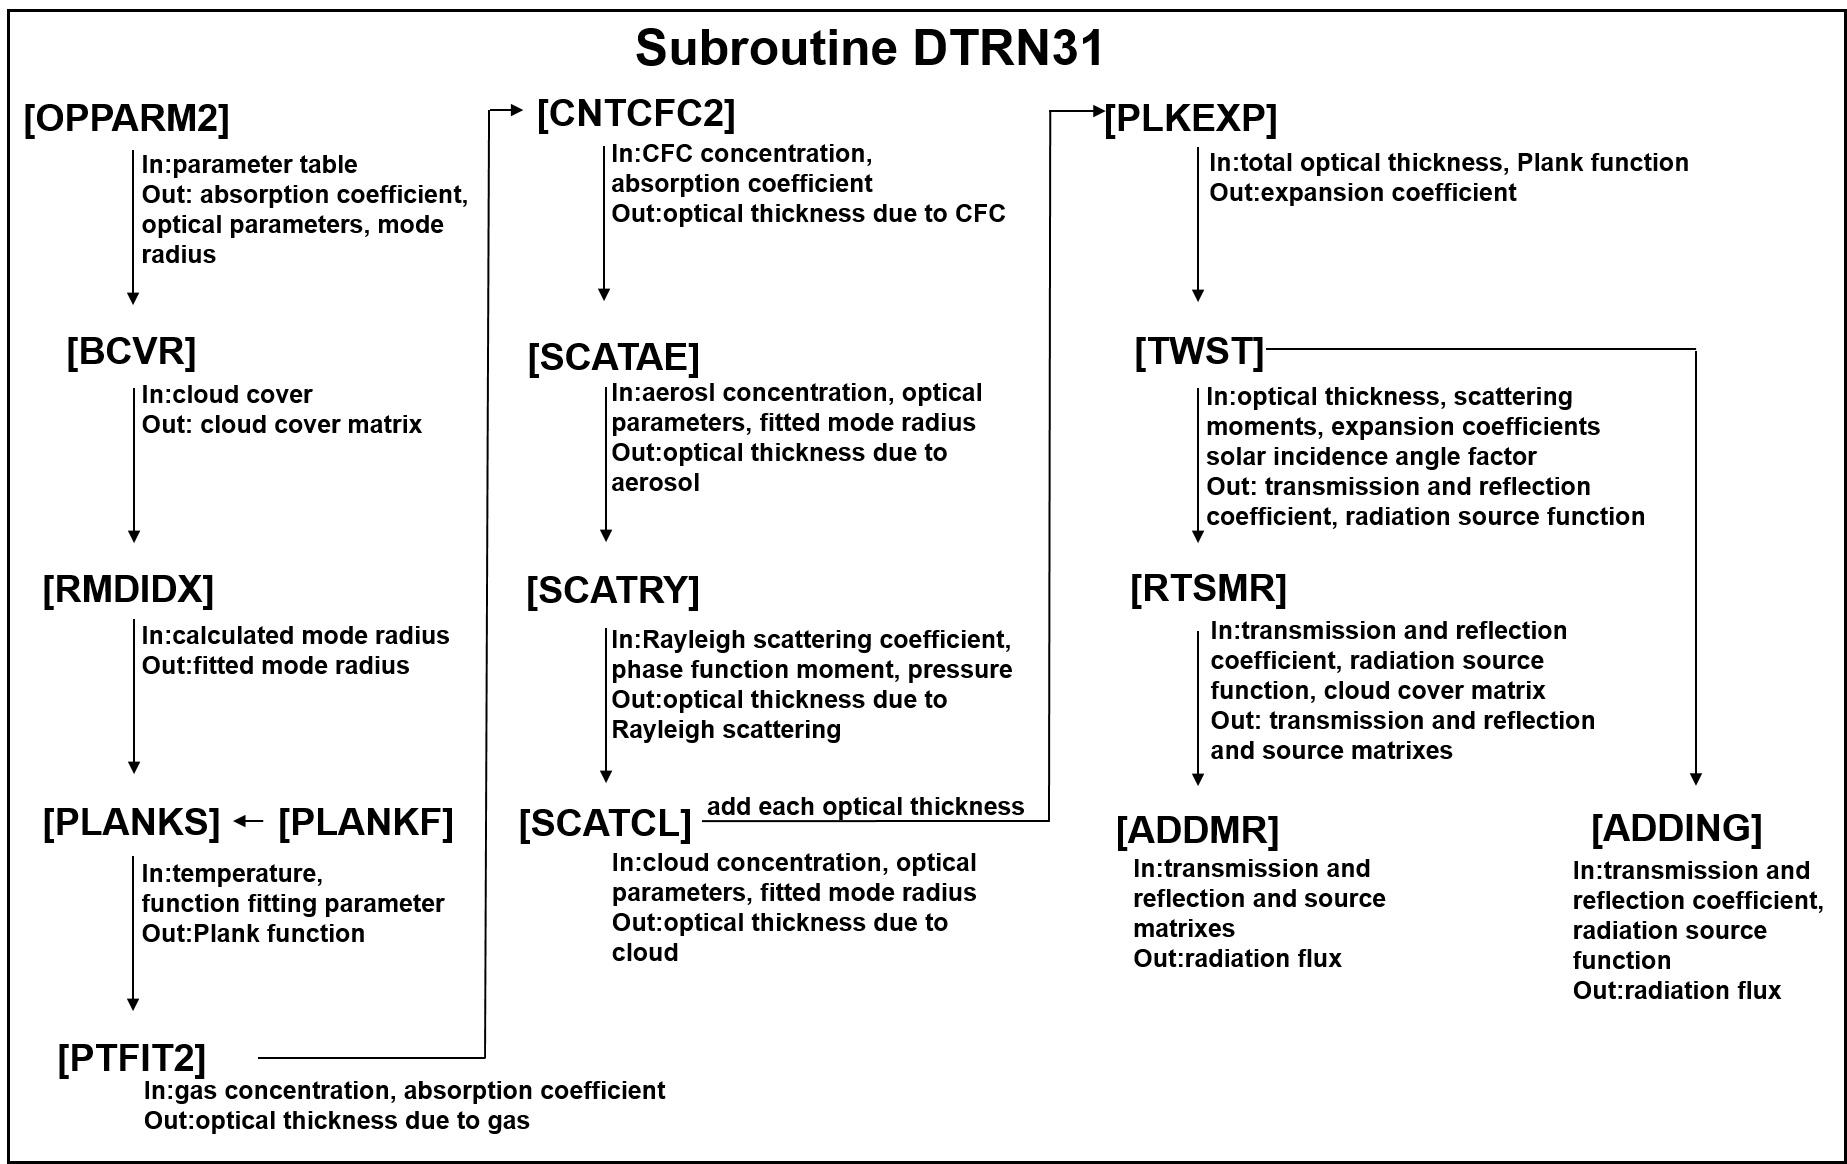
\includegraphics{Prad_Fig1.png}
\caption{Flowchart of \texttt{SUBROUTINE:{[}DTRN31{]}}}
\end{figure}

To account for the partial coverage of clouds, the transmission and
reflection coefficients and source functions for each layer are
calculated at weighted average of the cloud cover, separately for cloud
cover and clear-sky conditions. The cloud cover of the cumulus is also
considered. In addition, it also performs several adding and calculates
the clear-sky radiation flux.

\hypertarget{wavelength-and-sub-channel}{%
\subsubsection{Wavelength and
Sub-channel}\label{wavelength-and-sub-channel}}

The basics of radiative flux calculations are represented by
Beer-Lambert's Law.

\begin{eqnarray}
  F^\lambda(z) = F^\lambda(0) exp (-k^\lambda z)
\end{eqnarray}

\(F^{\lambda}\) is the radiant flux density at the wavelength of
\(\lambda\) and \(k^{\lambda}\) is the absorption coefficient. In order
to calculate the radiative fluxes related to the heating rate, the
integration operation with respect to the wavelength is required.

\begin{eqnarray}
  F(z) = \int F^\lambda(z) d \lambda= \int F^\lambda(0) exp (-k^\lambda z) d \lambda\
\end{eqnarray}

However, it is not easy to calculate this integration precisely because
the absorption and emission of radiation by gas molecules have the
complicated wavelength dependence of the absorption line attributed to
the structure of the molecule. The k-distribution method is a method
designed to make the relatively precise calculation easier. Within a
certain wavelength range, considering the density function \(F(k)\) for
\(\lambda\) of the absorption coefficient of \(k\), the above formula is
approximated as follows, \begin{eqnarray}
 \int F^\lambda(0) exp (-k^\lambda z) d \lambda
 \simeq \int \bar{F}^k(0) exp (-k z) F(k) dk
\end{eqnarray} where \(\bar{F}^k(0)\) is the flux averaged over a wavelength having
the absorption coefficient in this wavelength \(k\) in \(z=0\).

If \(\bar{F}^k(0)\) and \(F(k)\) are a relatively smooth functions to
the \(k\), \begin{eqnarray}
 \int F^\lambda(0) exp (-k^\lambda z) d \lambda
 \simeq \sum \bar{F}^i(0) exp (-k^i z) F^i
\end{eqnarray} the formula, as such above, can be relatively precisely calculated by
the addition of a finite number (sub-channels) of exponential terms.
This method has furthermore the advantage easy to consider the
absorption and scattering at the same time.

In the MIROC 6.0, by changing the radiation parameter data, the
calculations can be performed at various wavelengths. In the standard
version, the wavelength range is divided into 29 parts. In addition,
each wavelength range is divided into 1 to 6 sub-channels (corresponding
to the \(i\) in the above formula). There are 111 channels in total. The
wavelength range is divided by the wavenumber ( \(\mathrm{cm}^{-1}\) ),
1, 250, 400, 530, 610, 670, 750, 820, 980, 1175, 1225, 1325, 1400, 2000,
2500, 3300, 3800, 4700, 5200, 6000, 10000, 12750, 13250, 14750, 23000,
30000, 33500, 36000, 43500, 50000. Additionally, a chemical version is
also with 37 bands and 126 channels for chemical transport model and the
boundary of the shortwave region is also changed to 54000
\(\mathrm{cm}^{-1}\).

\hypertarget{calculation-of-the-planck-function}{%
\subsubsection{Calculation of the Planck
function}\label{calculation-of-the-planck-function}}

In this section, \texttt{SUBROUTINE:{[}PLANKS,\ PLANKF{]}} in pradt.F is
described.

The Planck function \(\bar{B}^{w}(T)\), integrated in each wavelength
range, is evaluated by the following formula. \begin{equation}
\bar{B}^{w}(T)=\lambda^{-2}{Texp}\left\{\sum_{n=1}^{5} B_{n}^{w}\left(\bar{\lambda}^{w} T\right)^{-n}\right\}
\end{equation} where \(\bar{\lambda}^{w}\) is the averaged wavelength of the
wavelength range, \(B_{n}^{w}\) is the parameter determined by function
fitting. This is calculated to the atmospheric temperature of each layer
\(T_l\), and the boundary atmospheric temperature of each layer
\(T_{l+1/2}\), surface temperature \(T_g\) and temperature
\(1\mathrm{K}\) higher than surface temperature \(T_{g+1K}\). The
calculations are performed for each wavelength and each layer. In the
following description, the subscript of the wavelength range \(w\) is
omitted.

\hypertarget{calculation-of-the-optical-thickness-to-gas-absorption}{%
\subsubsection{Calculation of the optical thickness to gas
absorption}\label{calculation-of-the-optical-thickness-to-gas-absorption}}

In this section, \texttt{SUBROUTINE:{[}PTFIT2{]}} in pradt.F is
described.

The optical thickness of the gas absorption (the line and continuum
absorption are unified) \(\tau^{K D}\) is expressed as follows by using
the index \(m\) as the type of molecules. \begin{equation}
\tau^{KD}=\sum_{m=1} k^{(m)} C^{(m)}
\end{equation} where \(k^{(m)}\) is the absorption coefficient of the molecule
\(m\), which is different for each sub-channel and determined as a
function of temperature \(T\) and atmospheric pressure \(p\).
\(C^{(m)}\) represents the amount of gas in the layer represented by
\(\mathrm{mol} / \mathrm{cm}^{2} / \mathrm{km}\), calculated by using
the gas concentration \(r^{(m)}\) in ppmv (
\(C^{(m)}=10^{-1} r^{(m)} \rho d z\) ). In the MIROC 6.0, the number of
the considered molecule types \(m\) is 6
(1:\(\mathrm{H}_{2} \mathrm{O}\), 2:\(\mathrm{C}\mathrm{O}_{2}\),
3:\(\mathrm{O}_{3}\), 4:\(\mathrm{N}_{2} \mathrm{O}\),
5:\(\mathrm{C}\mathrm{H}_{4}\), 6:\(\mathrm{O}_{2}\)). Also, \(k^{(m)}\)
is represented as follows (the details are in Sekiguchi and Nakajima,
2008). \begin{equation}
k^{(m)}=\exp \left(\log 10 k_{2}^{(m)}+(A+B T) \log \left(T / T_{\text {ref2 } }\right)\right)
\end{equation}

\begin{equation}
B=\left[\frac{\log 10\left(k_{3}^{(m)}-k_{2}^{(m)}\right)}{\log \left(\frac{T_{r e f 3}}{T_{r e f 2}}\right)}-\frac{\log 10\left(k_{1}^{(m)}-k_{2}^{(m)}\right)}{\log \left(\frac{T_{\text {ref1} }}{T_{\text {ref2}}}\right)}\right] /\left(T_{\text {ref3}}-T_{\text {ref1 }}\right)
\end{equation}

\begin{equation}
A=\frac{\log 10\left(k_{3}^{(m)}-k_{2}^{(m)}\right)}{\log \left(T_{\text {ref3 } } / T_{\text {ref2 } }\right)}-B T_{\text {ref3 }}
\end{equation}

\$ T\_ \{ref1-3\}\$ are the reference temperatures prepared in advance
(200, 260, 320 \(K\)), and \(k_{1-3}^{(m)}\) are the absorption
coefficients when the reference temperatures \$ T\_\{ref1-3\}\$ is used
(also fitted at 26 atmospheric pressure grids).

When considering the absorption of \(\mathrm{H}_{2} \mathrm{O}\), we
calculate the optical thickness of the self-broadening and add
\(\tau^{self}\). \begin{equation}
\tau^{K D\left(\mathrm{H}_{2} \mathrm{O}\right)}=\tau^{K D\left(\mathrm{H}_{2} \mathrm{O}\right)}+\tau^{\text {self }}
\end{equation}

\begin{equation}
\tau^{\text {self }}=\frac{k^{\left(\mathrm{H}_{2} \mathrm{O}_{-} \mathrm{self}\right)} C^{\left(\mathrm{H}_{2} \mathrm{O}\right)^{2}}}{C^{\left(\mathrm{H}_{2} \mathrm{O}\right)}+\rho d z 10^{5}}
\end{equation}

\(k^{(\mathrm{H}_{2} \mathrm{O}_{-} \mathrm{self})}\) is calculated in
the same way as \(k^{(m)}\). The self-broadening absorption coefficients
in the reference temperatures \(T_{ref1-3}\) are prescribed and
dependent on the pressure. In the above formula, \(10^{5}\) is
multiplied to convert the unit from \(\mathrm{km}\) to \(\mathrm{cm}\).
This calculation is done for each sub-channel and each layer.

\hypertarget{calculation-of-the-optical-thickness-to-cfc-absorption}{%
\subsubsection{Calculation of the optical thickness to CFC
absorption}\label{calculation-of-the-optical-thickness-to-cfc-absorption}}

In this section, \texttt{SUBROUTINE:{[}CNTCFC2{]}} in pradt.F is
described.

The optical thickness of the CFC absorption \(\tau^{CFC}\) is considered
for several types of CFCs \(m\). \begin{equation}
\tau^{C F C}=\sum_{m} 10^{k^{(m)}} r^{(m)} \rho \Delta z 10^{-1}
\end{equation} In MIROC 6.0, the number of the considered CFCs \(m\) is 28
(1:\(\mathrm{CFC\text{-11}}\), 2:\(\mathrm{CFC\text{-12}}\),
3:\(\mathrm{CFC\text{-13}}\), 4:\(\mathrm{CFC\text{-14}}\),
5:\(\mathrm{CFC\text{-113}}\), 6:\(\mathrm{CFC\text{-114}}\),
7:\(\mathrm{CFC\text{-115}}\), 8:\(\mathrm{HCFC\text{-21}}\),
9:\(\mathrm{HCFC\text{-22}}\), 10:\(\mathrm{HCFC\text{-123}}\),
11:\(\mathrm{HCFC\text{-124}}\), 12:\(\mathrm{HCFC\text{-141b}}\),
13:\(\mathrm{HCFC\text{-142b}}\), 14:\(\mathrm{HCFC\text{-225ca}}\),
15:\(\mathrm{HCFC\text{-225cb}}\), 16:\(\mathrm{HFC\text{-32}}\),
17:\(\mathrm{HFC\text{-125}}\), 18:\(\mathrm{HFC\text{-134}}\),
19:\(\mathrm{HFC\text{-134a}}\), 20:\(\mathrm{HFC\text{-143a}}\),
21:\(\mathrm{HFC\text{-152a}}\), 22:\(\mathrm{S}\mathrm{F}_{6}\),
23:\(\mathrm{ClON}\mathrm{O}_{2}\), 24:\(\mathrm{C}\mathrm{Cl}_{4}\),
25:\(\mathrm{N}_{2}\mathrm{O}_{5}\),
26:\(\mathrm{C}_{2}\mathrm{F}_{6}\), 27:\(\mathrm{HN}\mathrm{O}_{4}\),
28:\(\mathrm{SF}_{5}\mathrm{CF}_{3}\)). In the above formula,
\(10^{-1}\) is multiplied to convert from \(\mathrm{km}\) to
\(\mathrm{cm}\), and from ppmv to ratio. This calculation is done for
each sub-channel and each layer. This calculation is performed for each
layer and the wavelength range from about 540 to 1800
\(\mathrm{cm}^{-1}\).

\hypertarget{optical-thickness-to-scattering-and-scattering-moment}{%
\subsubsection{Optical thickness to scattering and scattering
moment}\label{optical-thickness-to-scattering-and-scattering-moment}}

Calculate the optical thickness of scattering and the scattering moment.
These calculations are performed for each wavelength and each layer. The
optical parameters for the particle matter \(q_{m}^{(p)}\) are prepared,
including the extinction coefficient (\(m = 1\)) including the
scattering and absorption process and the absorption coefficient
(\(m = 2\)) the moments of the volume scattering phase function
(\(m=3\text{-}4\): first-second order).

\hypertarget{aerosol}{%
\paragraph{Aerosol}\label{aerosol}}

In this section, \texttt{SUBROUTINE:{[}SCATAE{]}} in pradt.F is
described.

The optical thickness \(\tau^{a e}\), the part of the optical thickness
due to absorption \(\tau_{ab}^{a e}\), the scattering moment
\(Q_{m}^{a e}\) for aerosol are \begin{equation}
\tau^{a e}=\sum_{p} q_{1, n}^{(p)} r^{(p)} \times \rho \Delta z 10^{-1}
\end{equation}

\begin{equation}
\tau_{ab}^{a e}=\sum_{p} q_{2, n}^{(p)} r^{(p)} \times \rho \Delta z 10^{-1}
\end{equation}

\begin{equation}
Q_{m}^{a e}=\sum_{p} q_{m, n}^{(p)} r^{(p)} \times \rho \Delta z 10^{-1} (\mathrm{~m} \geq 3)
\end{equation}

\(p\) is the aerosol type, and \(r^{(p)}\) is volume mixing ratio of the
particle. The optical parameters for the particle \(q_{m, n}^{(p)}\)
depend on the mode radius index \(n\) prescribed for each particle
(IRA). In the MIROC 6.0, the number of the considered aerosol types
\(p\) 15 (1-6:soil dust (bin1-6), 7:carbonaceous (BC/OC=0.3),
8:carbonaceous (BC/OC=0.15), 9:carbonaceous (BC/OC=0), 10:black carbon
(external mixture), 11:sulfate, 12-15:sea salt (bin 1-4)).

If the aerosol radius is used, the optical thickness \(\tau^{a e}\), the
part of the optical thickness due to absorption \(\tau_{ab}^{a e}\), and
the scattering moment \(Q_{m}^{a e}\) for the hygroscopic aerosols
(e.g., carbonaceous, sulfate, sea salt) are \begin{equation}
\tau^{a e}=\sum_{p}\left[\left(1-F X_{a e}\right) q_{1, n f i t}^{(p)} r^{(p)}+F X_{a e} q_{1, n f i t+1}^{(p)} r^{(p)}\right] \times \rho \Delta z 10^{-1}
\end{equation}

\begin{equation}
\tau_{ab}^{a e}=\sum_{p}\left[\left(1-F X_{a e}\right) q_{2, n f i t}^{(p)} r^{(p)}+F X_{a e} q_{2, n f i t+1}^{(p)} r^{(p)}\right] \times \rho \Delta z 10^{-1}
\end{equation}

\begin{equation}
Q_{m}^{a e}=\sum_{p}\left[\left(1-F X_{a e}\right) q_{m, n f i t}^{(p)} r^{(p)}+F X_{a e} q_{m, n f i t+1}^{(p)} r^{(p)}\right] \times \rho \Delta z 10^{-1}(\mathrm{~m} \geq 2)
\end{equation}

\begin{equation}
F X_{a e}=\left(R H-R H_{n f i t}^{(r e f)}\right)\left(\frac{1}{R H_{n f i t+1}^{(r e f)}-R H_{n f i t}^{(r e f)}}\right)
\end{equation}

where \(RH\) is the local relative humidity and
\(R H_{n f i t}^{(r e f)}\) is the relative humidity given in the
parameter and \(nfit\) is the number of the prescribed relative humidity
closest to the \(RH\). \(nfit\) and \(FX_{ae}\) are calculated in the
\texttt{SUBROUTINE:{[}RMDIDX{]}} in pradt.F and determined in advance.
In the above formulas, \(10^{-1}\) is multiplied to convert from
\(\mathrm{km}\) to \(\mathrm{cm}\), and from ppmv to ratio.

\hypertarget{rayleigh-scattering-scatry}{%
\paragraph{\texorpdfstring{Rayleigh scattering
\texttt{{[}SCATRY{]}}}{Rayleigh scattering {[}SCATRY{]}}}\label{rayleigh-scattering-scatry}}

In this section, \texttt{SUBROUTINE:{[}SCATRY{]}} in pradt.F is
described.

The optical thickness \(\tau^{r}\) of Rayleigh scattering and the part
of the optical thickness due to absorption \(\tau_{ab}^{r}\) are

\begin{equation}
\tau^{r}=\frac{e^{r} d p q m o l_{1}}{p_{S T D}}
\end{equation}

\begin{equation}
\tau_{ab}^{r}=\frac{e^{r} d p q m o l_{2}}{p_{S T D}}
\end{equation}

\begin{equation}
p_{S T D}=1013.25
\end{equation}

where \(e^{r}\) is the Rayleigh scattering coefficient, \(qmol_m\) is
the moments of the phase function. These calculations are performed up
to \(m=2\). Also, this is added to the optical thickness for the
aerosol. \begin{equation}
\tau^{a e+r}=\tau^{a e}+\tau^{r}
\end{equation}

\begin{equation}
\tau_{ab}^{a e+r}=\tau_{ab}^{a e}+\tau_{ab}^{r}
\end{equation}

\hypertarget{cloud}{%
\paragraph{Cloud}\label{cloud}}

In this section, \texttt{SUBROUTINE:{[}SCATCL{]}} in pradt.F is
described.

The optical thickness \(\tau^{cl}\), the part of the optical thickness
due to absorption \(\tau_{ab}^{cl}\), and the scattering moment
\(Q_{m}^{c l}\) for cloud are \begin{equation}
\tau^{c l}=\sum_{c t} q_{1, n}^{(c t)}r^{(c t)}\times \rho \Delta z 10^{-1}
\end{equation}

\begin{equation}
\tau_{ab}^{c l}=\sum_{c t} q_{2, n}^{(c t)}r^{(c t)}\times \rho \Delta z 10^{-1}
\end{equation}

\begin{equation}
Q_{m}^{c l}=\sum_{c t} q_{m, n}^{(c t)} \times r^{(c t)} \rho \Delta z 10^{-1}(\mathrm{~m} \geq 3)
\end{equation}

\(ct\) is the cloud particle type (1:liquid cloud, 2:ice cloud). The
optical parameters for the particle \(q_{m, n}^{(c t)}\) depend on the
mode radius index \(n\) prescribed for each particle (IRC). If the cloud
radius is used, the optical thickness \(\tau^{cl}\), the part of the
optical thickness due to absorption \(\tau_{ab}^{cl}\), and the
scattering moment \(Q_{m}^{c l}\) for cloud are \begin{equation}
\tau^{c l}=\sum_{c t}\left[\left(1-F X_{c l}\right) q_{1, n f i t}^{(c t)} r^{(c t)}+F X_{c l} q_{1, n f i t+1}^{(c t)} r^{(c t)}\right] \times \rho \Delta z 10^{-1}
\end{equation}

\begin{equation}
\tau_{ab}^{c l}=\sum_{c t}\left[\left(1-F X_{c l}\right) q_{2, n f i t}^{(c t)} r^{(c t)}+F X_{c l} q_{2, n f i t+1}^{(c t)} r^{(c t)}\right] \times \rho \Delta z 10^{-1}
\end{equation}

\begin{equation}
Q_{m}^{c l}=\sum_{c t}\left[\left(1-F X_{c l}\right) q_{m, n f i t}^{(c t)} r^{(c t)}+F X_{c l} q_{m, n f i t+1}^{(c t)} r^{(c t)}\right] \times \rho \Delta z 10^{-1}(\mathrm{~m} \geq 3)
\end{equation}

\begin{equation}
F X_{c l}=\left(R^{(c t)}-R_{n f i t}^{(r e f)}\right)\left(\frac{1}{R_{n f i t+1}^{(r e f)}-R_{n f i t}^{(r e f)}}\right)
\end{equation}

where \(R^{(ct)}\) is the calculated mode radius and
\(R_{n f i t}^{(r e f)}\) is the mode radius given in the parameter and
\(nfit\) is the number of the prescribed mode radius closest to the
\(R^{(ct)}\). \(nfit\) and \(FX_{cl}\) are calculated in the subroutine
\texttt{SUBROUTINE:{[}RMDIDX{]}} in pradt.F and determined in advance.
In the above formulas, \(10^{-1}\) is multiplied to convert from
\(\mathrm{km}\) to \(\mathrm{cm}\), and from ppmv to ratio.

Finally, the total optical thickness for particle scattering, Rayleigh
scattering and absorption \(\tau^p\) and the contribution of scattering
\(\tau^{scat}\) are obtained as follows. \begin{equation}
\tau^{P}=\tau^{c l}+\tau^{a e+r}
\end{equation}

\begin{equation}
\tau^{s c a t}=\tau^{P}-\left(T_{ab}^{c l}+T_{ab}^{a e+r}\right)
\end{equation}

In addition, the moments of the normalized phase function \(G\) are
calculated up to the three orders. The zeroth moment \(G_1\) is trivial
from the normalization condition of the phase function. The first and
second moments \(G_2\), \(G_3\), are referred as the asymmetry factor
\(g\) and the truncation factor \(f\). \begin{equation}
G_{1}=1.0
\end{equation}

\begin{equation}
G_{m-1}=\frac{Q_{m}^{c l}+Q_{m}^{ae}}{\tau^{s c a t}}(m \geq 3), \quad G_{2}=g, \quad G_{3}=f
\end{equation}

This calculation is divided into the cloudy, clear sky and cumulus
conditions. In the cloudy and cumulus conditions, \(\tau^{cl}\) in the
0.5 and 0.67 \(\mathrm{{\mu}m}\) regions is as recorded as
\(\tau^{vis}\) in subroutine DTRN31.

**\(R^{ct}\) is calculated in \texttt{SUBROUTINE:RADFLX} as follows. \begin{equation}
R^{(c t)}=\left(\frac{3}{4 \pi} \frac{\rho r^{(c t)}}{\rho_{w}^{(c t)} n_{c}^{(c t)}}\right)^{1 / 3}
\end{equation} \(\rho_{w}^{(c t)}\) is the liquid or ice density. \(r^{ct}\) is the
amount of the liquid or ice cloud and calculated as follows. \begin{equation}
r^{(c t)}=\frac{C_{s t} r_{s t}^{(c t)}+C_{c u} r_{c u}^{(c t)}}{1-\left(1-C_{s t}\right)\left(1-C_{c u}\right)}
\end{equation} \(C\) is the area of the cloud, and the subscript \(st\) and \(cu\)
mean the stratus and cumulus. When \(r_{s t, c u}^{(c t)}\) is the small
amount in the stratosphere, it is reset to 0. \(n_{c}^{(c t)}\) is the
number density of cloud particles. \begin{equation}
n_{c}^{(l i q)}=\max \left(\frac{q_{a e}^{l i q} p N_{A}}{R T_{v}\left(18 \times 10^{-3} R_{v} / R\right)}, f_{l i q} n_{\min }^{(l i q)}\right)
\end{equation}

\begin{equation}
n_{c}^{(i c e)}=\max \left(\frac{q_{a e}^{i c e} p N_{A}}{R T_{v}\left(18 \times 10^{-3} R_{v} R_{v} / R\right)},\left(1-f_{l i q}\right) n_{\min }^{(i c e)}\right)
\end{equation}

where \(q_{a e}^{l i q}\) is the mixing ratio of the aerosol particles
calculated by the SPRINTERS and converted to the number concentration,
and \(n_{\min }^{(c t)}\) is the minimum number of the cloud particles.
and \(f_{liq}\) is liquid fraction. Also, \(n_{c}^{(c t)}\) is
calculated as follows when using OPT\_AECL\_SIMPLE. \begin{equation}
n_{c}^{(c t)}=\frac{\varepsilon n_{a} n_{m a x}^{(c t)}}{\varepsilon n_{a}+n_{\max }^{(c t)}}
\end{equation} where \(n_a\) is the number density of aerosol particles give as an
external condition, and \(\varepsilon\) and \(n_{\max }^{(c t)}\) are
constants. \(f_{liq}\) is calculated by the following formula using the
amount of cloud water \(w\) (\(0 \leq f_{\text {liq }} \leq 1\)). \begin{equation}
f_{l i q}=\frac{w_{s t} f_{l i q, s t}+w_{c u} f_{l i q, c u}}{w_{s t}+w_{c u}}
\end{equation}

\hypertarget{total-optical-thickness-dtrn31}{%
\subsubsection{\texorpdfstring{Total optical thickness
\texttt{{[}DTRN31{]}}}{Total optical thickness {[}DTRN31{]}}}\label{total-optical-thickness-dtrn31}}

All optical thickness including gaseous band absorption, and scattering
is, \begin{equation}
\tau=\tau^{K D}+\tau^{C O N}+\tau^{P}
\end{equation} where because \(\tau^{K D}\) is different for each subchannel, the
calculation is done for each sub-channel and each layer, and divided
into the cloudy, clear sky, and cumulus conditions.

\hypertarget{expansion-of-the-plank-function}{%
\subsubsection{Expansion of the plank
function}\label{expansion-of-the-plank-function}}

In this section, \texttt{SUBROUTINE:{[}PLKEXP{]}} in pradt.F is
described.

In each layer, the Planck function \(B\) is expanded as follows and the
expansion coefficients \(b_0\), \(b_1\), and \(b_2\), are obtained. \begin{equation}
{B}\left(\tau^{\prime}\right)=b_{0}+b_{1} \tau^{\prime}+b_{2}\left(\tau^{\prime}\right)^{2}
\end{equation} Here, as \({B}\left(\tau^{\prime}\right)\), \(B\) at the top of each
layer (the boundary with the top layer) is used, and as \({B}(\tau)\),
\(B\) at the bottom edge of each layer (the boundary with the layer
below), and as \({B}(\tau / 2)\), the \(B\) at the representative level
of each layer. \begin{equation}
b_{0}=B(0)
\end{equation}

\begin{equation}
b_{1}=(4{~B}(\tau / 2)-{B}(\tau)-3{~B}(0)) / \tau
\end{equation}

\begin{equation}
b_{2}=2({~B}(\tau)-{B}(0)-2{~B}(\tau / 2)) / \tau^{2}
\end{equation}

\begin{figure}
\centering
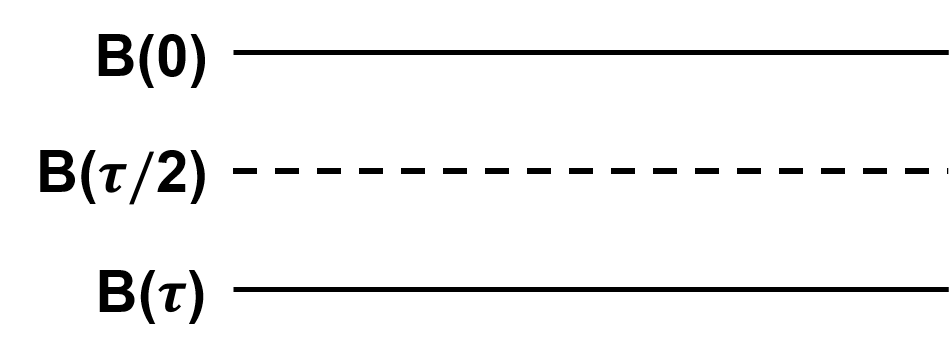
\includegraphics{Prad_Fig2.png}
\caption{Second-order expansion using the optical thickness of the plank
function}
\end{figure}

This calculation is done for each sub-channel and each layer and divided
into the cloudy, clear sky and cumulus conditions.

\hypertarget{transmission-and-reflection-coefficients-and-source-function}{%
\subsubsection{Transmission and reflection coefficients, and source
function}\label{transmission-and-reflection-coefficients-and-source-function}}

In this section, \texttt{SUBROUTINE:{[}TWST{]}} in pradt.F is described.

Using the obtained optical thickness \(\tau\), optical thickness of
scattering \(\tau^{scat}\), scattering moments \(g\), \(f\), expansion
coefficients for Planck function \(b_n\), and solar incidence angle
factor \(\mu_{0}\), the transmission coefficient \(T\), reflection
coefficient \(R\), downward radiation source function \(\epsilon^{+}\),
and the upward radiation source function \(\epsilon^{-}\) are founded,
by assuming a uniform layer and using the two-stream approximation.

The single-scattering albedo \(\omega\) is, \begin{equation}
\omega=\tau^{\text{scat}}/\tau
\end{equation} The optical thickness \(\tau^{*}\), the single-scattering albedo
\(\omega^{*}\), and asymmetric factor \(g^{*}\), corrected by the
contribution from the forward scattering factor \(f\) are, \begin{equation}
\tau^{*}=\tau(1-\omega f)
\end{equation}

\begin{equation}
\omega^{*}=\frac{(1-f) \omega}{1-\omega f}
\end{equation}

\begin{equation}
g^{*}=\frac{g-f}{1-f}
\end{equation}

\(\mu\) is a two-stream directional cosine. \begin{equation}
\mu \equiv\left(\frac{1}{\sqrt{3}}, \frac{1}{1.66}\right) \text { (shortwave, longwave) }
\end{equation}

\begin{equation}
W^{-} \equiv \mu^{-1 / 2}
\end{equation}

Furthermore, \begin{equation}
\hat{P}^{\pm}=\omega^{*} W^{-2}\left(1 \pm 3 g^{*} \mu^{2}\right) / 2
\end{equation}

\begin{equation}
\hat{S}_{s}^{\pm}=\omega^{*} W^{-}\left(1 \pm 3 g^{*} \mu_{0} \mu\right)
\end{equation}

can be determined as above as a normalized scattering phase function. \begin{equation}
\begin{aligned}
X &=\mu^{-1}-\left(\hat{P}^{+}-\hat{P}^{+}\right) \\
&=\mu^{-1}-3 \omega^{*} W^{-2} \mu^{2} g^{*} \\
\end{aligned}
\end{equation} \begin{equation}
\begin{aligned}
Y &=\mu^{-1}-\left(\hat{P}^{+}+\hat{P}^{+}\right) \\
&=\mu^{-1}-\omega^{*} W^{-2} \\
\end{aligned}
\end{equation}

\begin{equation}
\begin{aligned}
\hat{\sigma}_{S}^{+} &=\hat{S}_{S}^{+}+\hat{S}_{S}^{-} \\
&=\omega^{*} W^{-} \\
\end{aligned}
\end{equation}

\begin{equation}
\begin{aligned}
\hat{\sigma}_{S}^{-} &=\hat{S}_{s}^{+}-\hat{S}_{S}^{-} \\
&=3 \omega^{*} \mu_{0} W^{-} \mu g^{*}
\end{aligned}
\end{equation}

Using the above formula, the reflectance \(R\) and transmission \(T\)
become \begin{equation}
\begin{array}{c}
A A=\frac{X\left(1+e^{-\lambda \tau^{*}}\right)-\lambda\left(1-e^{-\lambda \tau^{*}}\right)}{X\left(1+e^{-\lambda \tau^{*}}\right)+\lambda\left(1-e^{-\lambda \tau^{*}}\right)} \\
\end{array}
\end{equation} \begin{equation}
\begin{array}{c}
B B=\frac{X\left(1-e^{-\lambda \tau^{*}}\right)-\lambda\left(1+e^{-\lambda \tau^{*}}\right)}{X\left(1-e^{-\lambda \tau^{*}}\right)+\lambda\left(1+e^{-\lambda \tau^{*}}\right)} \\
\end{array}
\end{equation}

\begin{equation}
\begin{array}{c}
\lambda=\sqrt{X Y} \\
\end{array}
\end{equation}

\begin{equation}
\begin{array}{c}
R=\frac{1}{2}(A A+B B) \\
\end{array}
\end{equation}

\begin{equation}
\begin{array}{c}
T=\frac{1}{2}(A A-B B)
\end{array}
\end{equation}

Next, we find the source function derived from the Planck function. \begin{equation}
\hat{b}_{n}=2 \pi\left(1-\omega^{*}\right) W^{-}\left(\frac{1}{1-\omega f}\right)^{n} b_{n}
\end{equation} The expansion coefficients of the radiation source function can be
found from the above formulas. \begin{equation}
\begin{array}{l}
D_{2}^{\pm}=\frac{\hat{b}_{2}}{Y} \\
\end{array}
\end{equation} \begin{equation}
\begin{array}{l}
D_{1}^{\pm}=\frac{\hat{b}_{1}}{Y} \mp \frac{2 \hat{b}_{2}}{X Y} \\
\end{array}
\end{equation}

\begin{equation}
\begin{array}{l}
D_{0}^{\pm}=\frac{\hat{b}_{0}}{Y}+\frac{2 \hat{b}_{2}}{X Y^{2}} \mp \frac{\hat{b}_{1}}{X Y} \\
\end{array}
\end{equation}

\begin{equation}
\begin{array}{l}
D^{\pm}\left(\tau^{*}\right)=D_{0}^{+}+D_{1}^{+} \tau^{*}+D_{2}^{+} \tau^{* 2}
\end{array}
\end{equation}

The radiation source function derived from the Planck function
\(\hat{\epsilon}_{A}^{\pm}\) is \begin{equation}
\begin{array}{l}
\hat{\epsilon}_{A}^{-}=D_{0}^{-}-R D_{0}^{-}-T D^{-}\left(\tau^{*}\right) \\
\end{array}
\end{equation} \begin{equation}
\begin{array}{l}
\hat{\epsilon}_{A}^{+}=D^{+}\left(\tau^{*}\right)-T D_{0}^{+}-R D^{-}\left(\tau^{*}\right)
\end{array}
\end{equation}

On the other hand, the radiation source function of the solar-induced
radiation is \begin{equation}
\begin{array}{l}
\hat{\epsilon}_{S}^{+}=F_{\text {sol }}\left(V_{s}^{+} e^{-\frac{\tau^{*}}{\mu_{0}}}-T V_{s}^{+}-R V_{s}^{-} e^{-\frac{\tau^{*}}{\mu_{0}}}\right)
\end{array}
\end{equation} \begin{equation}
\begin{array}{l}
\hat{\epsilon}_{S}^{+}=F_{\text {sol }}\left(V_{s}^{+} e^{-\frac{\tau^{*}}{\mu_{0}}}-T V_{s}^{+}-R V_{s}^{-} e^{-\frac{\tau^{*}}{\mu_{0}}}\right)
\end{array}
\end{equation}

Here, \(Q \gamma\) and \(V_{s}^{\pm}\) are expressed by the following
formulas, and \(F_{sol}\) is solar irradiance. \begin{equation}
\begin{array}{c}
V_{s}^{\pm}=\frac{1}{2}\left[Q \gamma \pm\left(\frac{Q \gamma}{\mu_{0}}+\frac{\hat{\sigma}_{S}^{-}}{X}\right)\right] \\
\end{array}
\end{equation} \begin{equation}
\begin{array}{c}
Q \gamma=\frac{X \hat{\sigma}_{S}^{+} \mu_{0}+\mu_{0}^{-1} \hat{\sigma}_{S}^{-}}{X Y \mu_{0}+\mu_{0}^{-1}}
\end{array}
\end{equation}

The direct solar transmission is also calculated in this subroutine. \begin{equation}
E x^{d i r}=e^{-\tau^{*}/ \mu_{0}}
\end{equation} This calculation is done for each sub-channel and each layer and
divided into the cloudy, clear sky, and cumulus conditions.

\hypertarget{t-r-s-matrixes-for-maximalrandom-approximation}{%
\subsubsection{T, R, S matrixes for maximal/random
approximation}\label{t-r-s-matrixes-for-maximalrandom-approximation}}

In this section, \texttt{SUBROUTINE:{[}RTSMR{]}} in pradt.F is
described.

In this subroutine, T, R, S matrixes for maximal/random approximation is
made. The radiation source function, which is the sum of both the plank
function and the solar incident origins, is \begin{equation}
\begin{array}{l}
\epsilon^{-(\text {cloud})}=\hat{\epsilon}_{S}^{-(\text {cloud})} {Tr}^{(\text {cloud})}+\hat{\epsilon}_{A}^{-(\text {cloud})} C \\
\end{array}
\end{equation} \begin{equation}
\begin{array}{l}
\epsilon^{-(\text {clear})}=\hat{\epsilon}_{S}^{-(\text {clear})}{Tr}^{(\text {clear})}+\hat{\epsilon}_{A}^{-(\text {clear})}(1-C) \\
\end{array}
\end{equation}

\begin{equation}
\begin{array}{l}
\epsilon^{+(\text {cloud})}=\hat{\epsilon}_{S}^{+(\text {cloud})}{Tr}^{(\text {cloud})}+\hat{\epsilon}_{A}^{-(\text {cloud})} C \\
\end{array}
\end{equation}

\begin{equation}
\begin{array}{l}
\epsilon^{+(\text {clear})}=\hat{\epsilon}_{S}^{+(\text {clear})}{Tr}^{(\text {clear})}+\hat{\epsilon}_{A}^{-(\text {clear})}(1-C)
\end{array}
\end{equation}

\(Tr\) is the direct solar transmission for maximal/random approximation
and calculated as follows in \texttt{SUBROUTINE:DTRN31}. \begin{equation}
\begin{aligned}
\operatorname{Tr}_{n}^{(\text {cloud})} &=E x_{n}^{(\text {cloud})} B_{n}^{(3)}+E x_{n}^{(\text {clear})}\left(1-B_{n}^{(1)}\right) \\
\end{aligned}
\end{equation} \begin{equation}
\begin{aligned}
E x_{n+1}^{(\text {cloud})} &={Tr}_{n}^{(\text {cloud})} E x_{n}^{\operatorname{dir}(\text {cloud})} \\
\end{aligned}
\end{equation}

\begin{equation}
\begin{aligned}
T r_{n}^{(\text {clear})} &=E x_{n}^{(\text {cloud})}\left(1-B_{n}^{(3)}\right)+E x_{n}^{(\text {clear})} B_{n}^{(1)} \\
\end{aligned}
\end{equation}

\begin{equation}
\begin{aligned}
E x_{n+1}^{(\text {clear)} }&={Tr}_{n}^{(\text {clear})} E x_{n}^{\text {dir}(\text {clear})}
\end{aligned}
\end{equation}

\(Ex\) is the cumulative direct solar transmission. \(B_{n}^{(1-4)}\) is
the cloud cover interaction index and calculated in
\texttt{SUBROUTINE:{[}BCVR{]}}in pradt.F . \begin{equation}
\begin{array}{l}
B_{n}^{(1)}=\frac{1-\max \left(C_{n-1}, C_{n}\right)}{1-C_{n-1}} \\
\end{array}
\end{equation} \begin{equation}
\begin{array}{l}
B_{n}^{(2)}=\frac{1-\max \left(C_{n+1}, C_{n}\right)}{1-C_{n+1}} \\
\end{array}
\end{equation}

\begin{equation}
\begin{array}{l}
B_{n}^{(3)}=\frac{\min \left(C_{n-1}, C_{n}\right)}{C_{n-1}} \\
\end{array}
\end{equation}

\begin{equation}
\begin{array}{l}
B_{n}^{(4)}=\frac{\min \left(C_{n+1}, C_{n}\right)}{C_{n+1}}
\end{array}
\end{equation}

Next, T matrixes for maximal/random approximation are calculated. \begin{equation}
\begin{array}{l}
T^{+(cloud, 1)}=T^{(\text {cloud})} B^{(3)} \\
\end{array}
\end{equation}

\begin{equation}
\begin{array}{l}
T^{+(\text {cloud}, 2)}=T^{(\text {cloud})}\left(1-B^{(1)}\right)\\
\end{array}
\end{equation}

\begin{equation}
\begin{array}{l}
T^{+(\text {clear}, 1)}=T^{(\text {clear})}\left(1-B^{(3)}\right)\\
\end{array}
\end{equation}

\begin{equation}
\begin{array}{l}
T^{+(\text {clear}, 2)}=T^{(\text {clear})} B^{(1)} \\
\end{array}
\end{equation}

\begin{equation}
\begin{array}{l}
T^{-(\text {cloud}, 1)}=T^{(\text {cloud})} B^{(4)} \\
\end{array}
\end{equation}

\begin{equation}
\begin{array}{l}
T^{-(\text {cloud}, 2)}=T^{(\text {cloud})}\left(1-B^{(2)}\right)\\
\end{array}
\end{equation}

\begin{equation}
\begin{array}{l}
T^{-(\text {clear}, 1)}=T^{(\text {clear})}\left(1-B^{(4)}\right)\\
\end{array}
\end{equation}

\begin{equation}
\begin{array}{l}
T^{-(\text {clear}, 2)}=T^{(\text {clear})} B^{(2)}
\end{array}
\end{equation}

Also, R matrixes for maximal/random approximation are calculated. \begin{equation}
\begin{array}{l}
R^{+(\text {cloud}, 1)}=R^{(\text {cloud})} B^{(3)} \\
\end{array}
\end{equation} \begin{equation}
\begin{array}{l}
R^{+(\text {cloud}, 2)}=R^{(\text {cloud})}\left(1-B^{(1)}\right) \\
\end{array}
\end{equation}

\begin{equation}
\begin{array}{l}
R^{+(\text {clear}, 1)}=R^{(\text {clear})}\left(1-B^{(3)}\right) \\
\end{array}
\end{equation}

\begin{equation}
\begin{array}{l}
R^{+(\text {clear}, 2)}=R^{(\text {clear})} B^{(1)} \\
\end{array}
\end{equation}

\begin{equation}
\begin{array}{l}
R^{-(\text {cloud}, 1)}=R^{(\text {cloud})} B^{(4)} \\
\end{array}
\end{equation}

\begin{equation}
\begin{array}{l}
R^{-(\text {cloud,2})}=R^{(\text {cloud})}\left(1-B^{(2)}\right) \\
\end{array}
\end{equation}

\begin{equation}
\begin{array}{l}
R^{-(\text {clear}, 1)}=R^{(\text {clear})}\left(1-B^{(4)}\right) \\
\end{array}
\end{equation}

\begin{equation}
\begin{array}{l}
R^{-(\text {clear}, 2)}=R^{(\text {clear})} B^{(2)}
\end{array}
\end{equation}

This calculation is done for each sub-channel and each layer.

\hypertarget{adding-of-source-functions-for-each-layer}{%
\subsubsection{Adding of source functions for each
layer}\label{adding-of-source-functions-for-each-layer}}

In this section, \texttt{SUBROUTINE:{[}ADDMR\ or\ ADDING} in pradt.F is
described.

By using transmission coefficient \(T\), reflection coefficient \(R\),
and radiation source function \(\varepsilon\) in all layers, the
radiation fluxes \(u\) at each layer boundary can be obtained by using
the adding method. This means that the when two layers of \(T\), \(R\),
\(\varepsilon\) are known, the \(T\), \(R\), \(\varepsilon\) of the
whole combined layer of the two layers can be easily calculated.

\begin{figure}
\centering
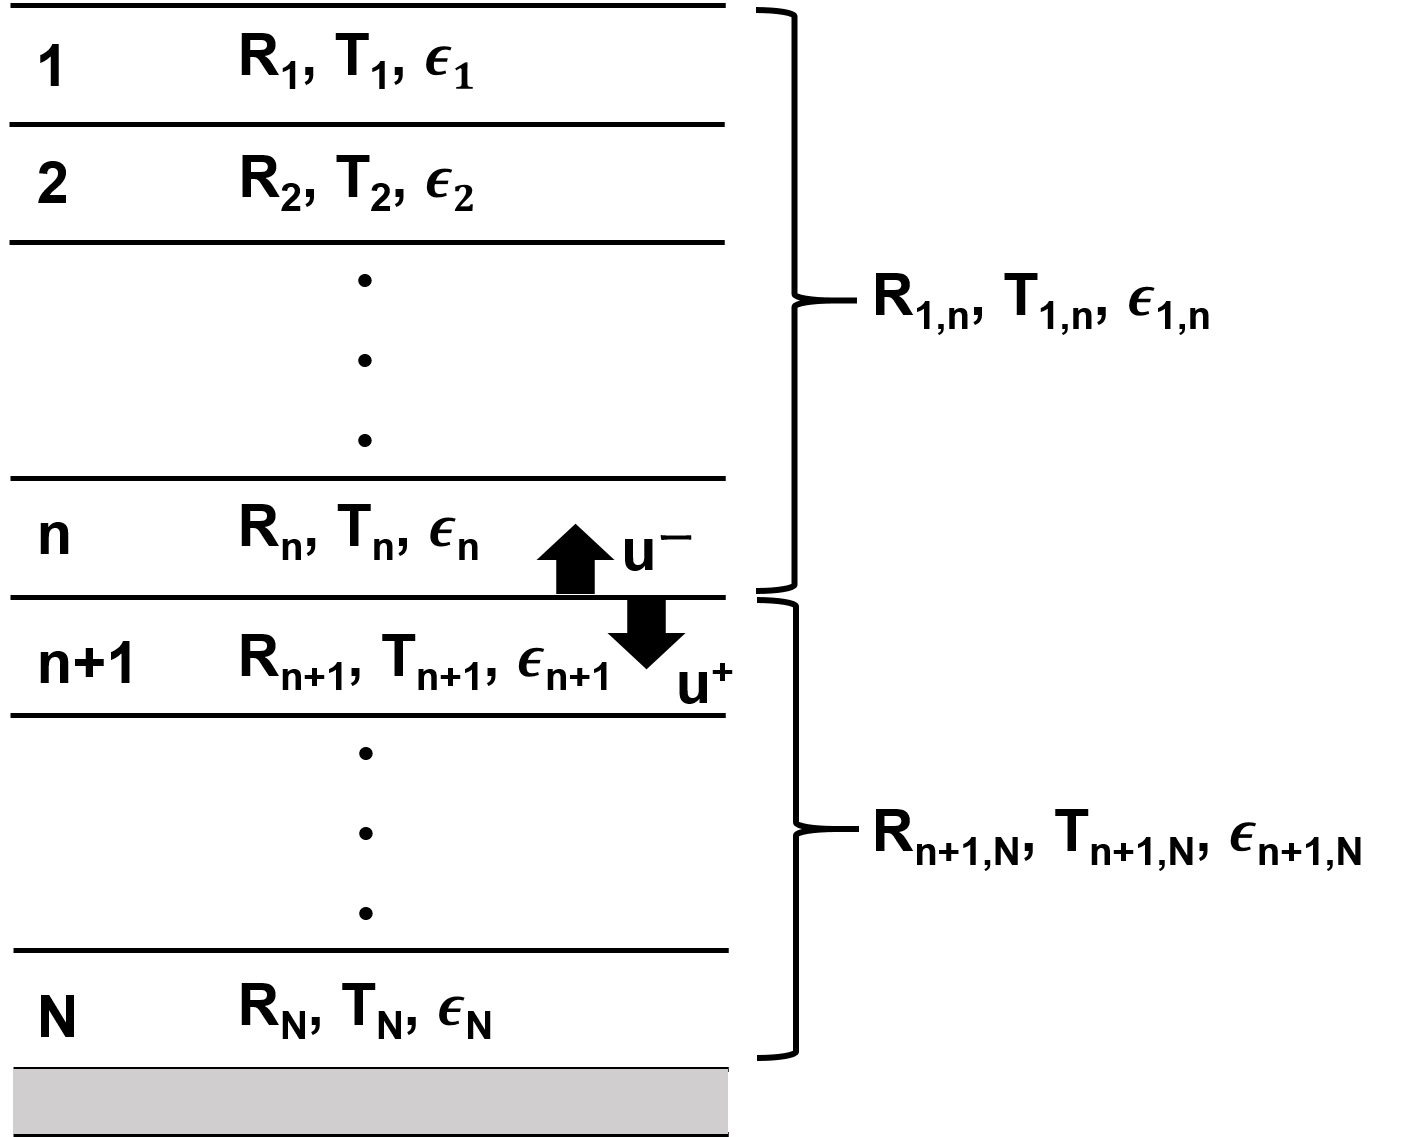
\includegraphics{Prad_Fig3.png}
\caption{Schematic illustration of the adding method}
\end{figure}

\hypertarget{subroutineaddmr}{%
\paragraph{\texorpdfstring{\texttt{SUBROUTINE:{[}ADDMR{]}}}{SUBROUTINE:{[}ADDMR{]}}}\label{subroutineaddmr}}

In this subroutine, the maximal/random flux in cloudy conditions is
calculated by the adding method and the T, R, and S matrixes are used
for calculations.

First, the upward radiation source function the bottom layer is
calculated.

In the shortwave region, \begin{equation}
\begin{array}{l}
\epsilon_{N}^{-(\text {cloud})}=W^{+} \alpha_{s} \mu_{0}\left(\frac{1}{\mu}\right) F_{0} e_{N}^{-\left\langle\tau^{*}\right\rangle / \mu_{0}(\text{cloud})} \\
\end{array}
\end{equation} \begin{equation}
\begin{array}{l}
\epsilon_{N}^{-(\text {clear})}=W^{+} \alpha_{s} \mu_{0}\left(\frac{1}{\mu}\right) F_{0} e_{N}^{-\left\langle\tau^{*}\right\rangle / \mu_{0} \text {(clear) }}
\end{array}
\end{equation}

\(\left\langle\tau^{*}\right\rangle\) indicates the total optical
thickness \(\tau^{*}\) of from the upper end of the atmosphere to the
upper end of the layer currently being considered and
\(e^{-\left\langle\tau^{*}\right\rangle / \mu_{0}}\) is calculated in
\texttt{SUBROUTINE:{[}ADDMR{]}} of pradt.F.

In the longwave region, \begin{equation}
\begin{array}{l}
\epsilon_{N}^{-(\text {cloud})}=\epsilon_{N}^{-(\text {cloud})}+W^{+} 2 \pi\left(1-\alpha_{s}\right) B_{N} C_{N} \\
\end{array}
\end{equation} \begin{equation}
\begin{array}{l}
\epsilon_{N}^{-(\text {clear})}=\epsilon_{N}^{-(\text {clear})}+W^{+} 2 \pi\left(1-\alpha_{s}\right) B_{N}\left(1-C_{N}\right)
\end{array}
\end{equation}

Here, \begin{equation}
W^{+} \equiv \mu^{1 / 2}
\end{equation} The reflectance \(R_{1, n}^{-}\) and source function
\(\epsilon_{1, n}^{+}\) regarded from the first to the \(n\) layers as a
single layer are \begin{equation}
\begin{array}{l}
\epsilon_{1, n}^{+}=\epsilon_{n}^{+}+T_{n}^{+}\left(1-R_{n}^{+} R_{1, n-1}^{-}\right)^{-1}\left(R_{1, n-1}^{-} \epsilon_{n}^{-}+\epsilon_{1, n-1}^{+}\right) \\
\end{array}
\end{equation} \begin{equation}
\begin{array}{l}
R_{1, n}^{-}=R_{n}^{-}+T_{n}^{+}\left(1-R_{n}^{+} R_{1, n-1}^{-}\right)^{-1} R_{1, n-1}^{-} T_{n}^{-}
\end{array}
\end{equation}

The upward and downward fluxes at the bottom of the atmosphere are \begin{equation}
\begin{array}{l}
u_{N+1 / 2}^{+}=\left(1-R_{1, N-1}^{-} R_{N}^{+}\right)^{-1}\left(\epsilon_{1, N-1}^{+}+R_{1, N-1}^{-} \epsilon_{N}^{-}\right) \\
\end{array}
\end{equation}

\begin{equation}
\begin{array}{l}
u_{N+1 / 2}^{-}=\left(1-R_{N}^{+} R_{1, N-1}^{-}\right)^{-1}\left(\epsilon_{N}^{-}+R_{N}^{+} \epsilon_{1, N-1}^{+}\right)
\end{array}
\end{equation}

Also, upward and downward fluxes at the boundary between layers \(n\)
and \(n+1\) are \begin{equation}
\begin{array}{l}
u_{n+1 / 2}^{+}=\left(1-R_{1, n-1}^{-} R_{n}^{+}\right)^{-1}\left(R_{1, n-1}^{-} T_{n}^{-} u_{n+1 / 2}^{-}+R_{1, n-1}^{-} \epsilon_{n}^{-}+\epsilon_{1, n}^{+}\right) \\
\end{array}
\end{equation} \begin{equation}
\begin{array}{l}
u_{n+1 / 2}^{-}=\left(1-R_{n}^{+} R_{1, n-1}^{-}\right)^{-1}\left(T_{n}^{-} u_{n+1 / 2}^{-}+R_{n}^{+} \epsilon_{1, n-1}^{+}+\epsilon_{n}^{-}\right)
\end{array}
\end{equation}

However, the upward and downward flux at the upper end of the atmosphere
is as follows. \begin{equation}
\begin{array}{l}
u_{1 / 2}^{+}=0 \\
\end{array}
\end{equation} \begin{equation}
\begin{array}{l}
u_{1 / 2}^{-}=T_{1}^{-} u_{1+1 / 2}^{-}+\epsilon_{1}^{-}
\end{array}
\end{equation}

Finally, since this flux is scaled, we rescaled and added the direct
solar incidence to the find the radiation flux. Furthermore, the flux in
the cloudy area and the clear sky area is added. \begin{equation}
\begin{array}{c}
F_{n+1 / 2}^{+}=\frac{W^{+}}{W}\left(u_{n+1 / 2}^{+(\text{cloud})}+u_{n+1 / 2}^{+(\text{clear})}\right)+\mu_{0} F_{0}\left(e_{n+1 / 2}^{-\left\langle\tau^{*}\right\rangle / \mu_{0}(\text {cloud})}\right) \\
\end{array}
\end{equation} \begin{equation}
\begin{array}{c}
F_{n+1 / 2}^{-}=\frac{W^{+}}{W}\left(u_{n+1 / 2}^{-(\text{cloud})}+u_{n+1 / 2}^{-(\text {clear})}\right)
\end{array}
\end{equation}

Also, surface direct downward radiation flux \(F_{s f}^{+}\) is \begin{equation}
F_{s f}^{+}=\mu_{0} F_{0}\left(e_{N}^{-\left\langle\tau^{*}\right\rangle / \mu_{0}(\text {cloud})}+e_{N}^{-\left\langle\tau^{*}\right\rangle / \mu_{0} \text{(clear)}}\right)
\end{equation} This calculation is done for each sub-channel.

\hypertarget{subroutineadding}{%
\paragraph{\texorpdfstring{\texttt{SUBROUTINE:{[}ADDING{]}}}{SUBROUTINE:{[}ADDING{]}}}\label{subroutineadding}}

Since the maximal/random approximation cannot be used under the clear
sky condition, this subroutine is used to calculate the flux.

First, the radiation source function, which is the sum of both the plank
function origin and the solar incident origin, is \begin{equation}
\epsilon^{\pm}=\hat{\epsilon}_{S}^{\pm} e^{-\left\langle\tau^{*}\right\rangle / \mu_{0}}+\hat{\epsilon}_{A}^{\pm}
\end{equation} There are layers \(1, 2,\dots, N\) from the top. The surface layer is
considered to be a single layer and the \(N\) layer. Given the
reflectance and source function of the layers from the n to the \(N\)
layer as a single layer \(R_{n, N}\), \(\epsilon_{n, N}^{-}\), \begin{equation}
\begin{array}{c}
R_{n, N}=R_{n, N}+T_{n}\left(1-R_{n+1, N} R_{n}\right)^{-1} R_{n+1} T_{n} \\
\end{array}
\end{equation} \begin{equation}
\begin{array}{c}
\epsilon_{n, N}^{-}=\epsilon_{n}^{-}+T_{n}\left(1-R_{n+1, N} R_{n}\right)^{-1}\left(R_{n+1, N} \epsilon_{n}^{+}+\epsilon_{n, N}^{-}\right)
\end{array}
\end{equation}

\begin{equation}
\begin{array}{c}
R_{n, N}=R_{n, N}+T_{n}\left(1-R_{n+1, N} R_{n}\right)^{-1} R_{n+1} T_{n} \\
\end{array}
\end{equation}

\begin{equation}
\begin{array}{c}
\epsilon_{n, N}^{-}=\epsilon_{n}^{-}+T_{n}\left(1-R_{n+1, N} R_{n}\right)^{-1}\left(R_{n+1, N} \epsilon_{n}^{+}+\epsilon_{n, N}^{-}\right)
\end{array}
\end{equation}

This can be solved by \(n=N-1,\dots,1\) in sequence, starting from the
values at the surface \(R_{N, N}\), \(\epsilon_{N, N}^{-}\). \begin{equation}
\begin{array}{c}
R_{N, N}=R_{N}=\alpha_{s} \\
\end{array}
\end{equation} \begin{equation}
\begin{array}{c}
\epsilon_{N, N}=W^{+}\left(\alpha_{s} \mu_{0}\left(\frac{1}{\mu}\right) e^{-\left\langle\tau^{*}\right\rangle / \mu_{0}} F_{0}+2 \pi\left(1-\alpha_{s}\right) B_{N}\right)
\end{array}
\end{equation}

The reflectance \(R_{1, n}\) and source function \(\epsilon_{1, n}^{+}\)
regarded from the first to the \(n\) layers as a single layer are \begin{equation}
\begin{array}{c}
R_{1, n}=R_{n}+T_{n}\left(1-R_{1, n-1} R_{n}\right)^{-1} R_{1, n-1} T_{n} \\
\end{array}
\end{equation} \begin{equation}
\begin{array}{c}
\epsilon_{1, N}^{+}=\epsilon_{n}^{+}+T_{n}\left(1-R_{1, n-1} R_{n}\right)^{-1}\left(R_{1, n-1} \epsilon_{n}^{-}+\epsilon_{1, n-1}^{+}\right)
\end{array}
\end{equation}

It can be solved by \(n=2,\dots, N\), starting from
\(R_{1,1}=R_{1}, \epsilon_{1,1}^{+}=\epsilon_{1}^{+}\).

With these, downward flux at the boundary between layers \(n\) and
\(n+1\), the downward and upward flux are came back to a problem between
two layers of combined layer, the combinations of layers \(1-n\) and
\(n+1-N\). \begin{equation}
\begin{array}{c}
u_{n+1 / 2}^{+}=\left(1-R_{1, n} R_{n+1, N}\right)^{-1}\left(\epsilon_{1, n}^{+}+R_{1, n} \epsilon_{n+1, N}^{-}\right) \\
\end{array}
\end{equation} \begin{equation}
\begin{array}{c}
u_{n+1 / 2}^{-}=R_{n+1, N} u_{n, n+1}^{+}+\epsilon_{n+1, N}^{-}
\end{array}
\end{equation}

can be written as above. However, the flux at the top of the atmosphere
is \begin{equation}
\begin{array}{c}
u_{1 / 2}^{+}=0 \\
\end{array}
\end{equation} \begin{equation}
\begin{array}{c}
u_{1 / 2}^{-}=\epsilon_{1, N}^{-}
\end{array}
\end{equation}

Finally, since this flux is scaled, we rescaled and added the direct
solar incidence to the find the radiation flux. \begin{equation}
\begin{array}{c}
F_{n+1 / 2}^{+}=\frac{W^{+}}{W} u_{n+1 / 2}^{+}+\mu_{0} e^{-\left\langle\tau^{*}\right\rangle / \mu_{0}} F_{0} \\
\end{array}
\end{equation} \begin{equation}
\begin{array}{c}
F_{n+1 / 2}^{-}=\frac{W^{+}}{W} u_{n+1 / 2}^{-}
\end{array}
\end{equation}

Also, surface direct downward radiation flux \(F_{s f}^{+}\) is \begin{equation}
F_{s f}^{+}=\mu_{0} F_{0} e^{-\left\langle\tau^{*}\rangle\ \mu_{0}\right.}
\end{equation}

\hypertarget{adding-in-the-flux}{%
\subsubsection{Adding in the flux}\label{adding-in-the-flux}}

\begin{equation}
F^{\pm}=\sum_{c} w_{c}\left(1-C_{c u}\right) \bar{F}^{\pm}+\sum_{c} w_{c} C_{c u} F^{c \pm}
\end{equation}

\begin{equation}
F^{\circ \pm}=\sum_{c} w_{c} F^{\circ \pm}
\end{equation}

If the radiation flux \(F_{C}^{\pm}\) is found for each sub-channel in
each layer, the wavelength-integrated flux is found by multiplying a
weight \(w_c\) correspondingly to a wavelength representative of the
sub-channel and adding. \(C_{cu}\) is the horizontal coverage of the
cumulus cloud. It is divided into the short wavelength range and long
wavelength range and added together. In addition, the downward flux of a
part of the short wavelength region (shorter than the wavelength of
0.7-0.8 \(\mathrm{{\mu}m}\)) at the surface is obtained as PAR
(photosynthetically active radiation). Also, the radiation flux in the
clear-sky condition is calculated (\(F^{\circ \pm}\)).

Also, in the shortwave region, we find the downward radiation at the
lower end of the atmosphere and the difference between the surface
direct downward radiation flux. \begin{equation}
F_{s f}^{+}=\sum_{c} w_{c}\left(1-C_{u}\right) \bar{F}_{N+1 / 2}^{+}+\sum_{c} w_{c} C_{c u} F_{N+1 / 2}^{c}
\end{equation}

\begin{equation}
F_{s f, d i f}^{+}=\sum_{c} w_{c}\left(1-C_{c u}\right)\left(\bar{F}_{N+1 / 2}^{+}-\bar{F}_{s f}^{+}\right)+\sum_{c} w_{c} C_{c u}\left(F_{N+1 / 2}^{c}-F_{s f}^{c}\right)
\end{equation}

This calculation is done in \texttt{SUBROUTINE:{[}DTRN31{]}}

\hypertarget{calculation-of-the-temperature-derivative-of-the-flux}{%
\subsubsection{Calculation of the temperature derivative of the
flux}\label{calculation-of-the-temperature-derivative-of-the-flux}}

To implicitly solve for surface temperature, calculate differential term
of upward flux with respect to surface temperature
\(\mathrm{d}F^{\mp}/dT_{g}\). Therefore, we obtained the value for
temperatures \(1\text{K}\) higher than \(T_g\)
\(\bar{B}^{w}\left(T_{g}+1\right)\) and used it to redo the flux
calculation using the addition method, and the difference from the
original value is set to \(\mathrm{d}F^{\mp}/dT_{g}\). This is a
meaningful value only in the longwave region (earth radiation region).
This calculation is done in \texttt{SUBROUTINE:{[}RADFLX{]}} of pradt.F.

\hypertarget{calculation-of-the-heating-rate}{%
\subsubsection{Calculation of the heating
rate}\label{calculation-of-the-heating-rate}}

The heating rate of the nth layer \(H_n\) is calculated by using the
radiation flux obtained so far. It is calculated separately for
shortwave and longwave ranges, and finally add together
(\texttt{SUBROUTINE:{[}RDTND{]}} in pradm.F). \begin{equation}
H_{n}=-\frac{\left(F_{n}^{-}-F_{n}^{-}\right)-\left(F_{n}^{+}-F_{n+1}^{+}\right)}{g C_{p} d p}
\end{equation}

\hypertarget{flux-of-incidence-and-incident-angle}{%
\subsubsection{Flux of incidence and incident
angle}\label{flux-of-incidence-and-incident-angle}}

In this section, \texttt{SUBROUTINE:{[}SHTINS{]}} in pradi.F is
described.

The following parameters are determined using the eccentricity \(e\),
with reference to Berger (1978). \begin{equation}
\begin{array}{l}
\beta=\sqrt{1-e^{2}} \\
\end{array}
\end{equation} \begin{equation}
\begin{array}{l}
a_{1}=-2\left(\frac{1}{2} e+\frac{1}{8} e^{3}\right)(1+\beta) \\
\end{array}
\end{equation}

\begin{equation}
\begin{array}{l}
a_{2}=-2\left(-\frac{1}{4} e^{2}\right)\left(\frac{1}{2}+\beta\right) \\
\end{array}
\end{equation}

\begin{equation}
\begin{array}{l}
a_{3}=-2\left(\frac{1}{8} e^{3}\right)\left(\frac{1}{2}+\beta\right) \\
\end{array}
\end{equation}

\begin{equation}
\begin{array}{l}
b_{1}=2 e-\frac{1}{4} e^{3} \\
\end{array}
\end{equation}

\begin{equation}
\begin{array}{l}
b_{2}=\frac{5}{4} e^{2} \\
\end{array}
\end{equation}

\begin{equation}
\begin{array}{l}
b_{3}=\frac{13}{12} e^{3}
\end{array}
\end{equation}

Additionally, \begin{equation}
\begin{array}{l}
\epsilon=\frac{e p s d}{180} \pi \\
\end{array}
\end{equation} \begin{equation}
\begin{array}{l}
\varpi=\frac{v p i d+180}{180} \pi
\end{array}
\end{equation}

where \(epsd\) and \(vpid\) are the angle of the obliquity and the
precession.

Earth position \(\lambda_{m}\) at a time \(t_m\) is represented by using
the position of the vernal equinox \(\lambda_{0}\). \begin{equation}
\begin{array}{c}
\lambda_{0}=a_{1} \sin (-\varpi)+a_{2} \sin (-2 \varpi)+a_{3} \sin (-3 \varpi) \\
\end{array}
\end{equation} \begin{equation}
\begin{array}{c}
\lambda_{m}=\frac{t_{m}-t_{0}}{2 \pi \times 365 \times 86400}+\lambda_{0}
\end{array}
\end{equation}

The solar declination \(\delta\) is \begin{equation}
\delta=\arcsin (\sin \epsilon \sin (V+\varpi))
\end{equation} \begin{equation}
\\V=\lambda_{m}-\varpi+b_{1} \sin \left(\lambda_{m}-\varpi\right)+b_{2} \sin 2\left(\lambda_{m}-\varpi\right)+b_{3} \sin 3\left(\lambda_{m}-\varpi\right)
\end{equation}

The incident angle \(\cos \zeta\) is founded by using the latitude
\(\varphi\), the solar declination \(\delta\), and the hour angle at a
point of longitude \(h\). \begin{equation}
\mu_{0}=\cos \zeta=\sin \varphi \sin \delta+\cos \varphi \cos \delta \cosh
\end{equation} Incident Flux \(F_0\) is represented as follows, \begin{equation}
\begin{array}{c}
F_{0}=F_{00} r^{-2} \\
\end{array}
\end{equation} \begin{equation}
\begin{array}{c}
r=\frac{1-e^{2}}{1+e(\cos V+\varpi)}
\end{array}
\end{equation}

where \(F_{00}\) is the solar constant and is the ratio of the ratio to
the time of the distance between the sun and the earth. The number of
times when \(\cos \zeta \geq 0\) (in the daytime) in time increments
(set in NHSUB), is counted, and \(F_{0}\) and \(\cos \zeta\) are finally
averaged.

It is also possible to give average annual insolation. In this case, the
annual and day mean incidence and angle of incidence are approximated as
follows. \begin{equation}
\begin{array}{c}
\bar{F}=F_{00} / \pi \\
\end{array}
\end{equation}

\begin{equation}
\begin{array}{c}
\bar{\mu}_{0} \simeq 0.410+0.590 \cos ^{2} \varphi
\end{array}
\end{equation}

\hypertarget{reading-the-each-parameter}{%
\subsubsection{Reading the each
parameter}\label{reading-the-each-parameter}}

In \texttt{SUBROUTINE:{[}OPPARM2{]}}of pradt.F, various parameters used
for radiation calculation are read. The outline of the procedure is
shown below.

\begin{enumerate}
\def\labelenumi{\arabic{enumi}.}
\item
  Read the numbers of bands, the radiances representative of upward and
  downward radiation, the grids of the pressure \(\log (\mathrm{p})\),
  grid of the temperatures, the optical flag, and CFCs.
\item
  Read the band boundaries and the information of the pressure grid and
  temperature grid.
\item
  First, the optical property flag, the number of channels, the weights
  for channels and the number of the molecules including in a waveband
  are read. The optical property flag is modified in order to
  distinguish the PAR, 0.67, 0.5, and 10.5 \(\mathrm{{\mu}m}\).
  Additionally, molecule ID and \(k\)-width are read for each molecule.
  Finally, the absorption coefficient for the self-broadening and CFC
  are also done only when the optical property flag in the band is
  positive. The k-width and the absorption coefficient for the
  self-broadening are arranged in the order of the grid of the
  temperatures, the grids of the pressures, and the channels. Step 3 is
  performed for each wavelength band.
\item
  First, the number of particles is read. Next, the numbers of the modes
  and the mode radius (or relative humidity) are read for each particle.
  Using the mode radius (or relative humidity), the following parameter
  required to interpolate the calculated values is calculated for each
  mode number. \begin{equation}
  \frac{1}{R_{n+1}^{(r e f)}-R_{n}^{(r e f)}}
  \end{equation}
\item
  Read the band boundaries again.
\item
  Read the Plank function coefficient, solar insolation, surface
  properties (not output), Rayleigh scattering coefficient, Rayleigh
  scattering phase function. The moment for particle scattering phase
  function is read in the order of the particle and the optical number
  and read up to the second moment. Step 6 is performed for each
  wavelength band.
\end{enumerate}

\hypertarget{other-notes}{%
\subsubsection{Other notes}\label{other-notes}}

The calculation of the radiation is usually not done at every step.
Thus, the radiation flux is saved, and it is used if the time is not
used for radiation calculation. As for the shortwave radiation, using
the percentage of time (time is \(\mu_{0}>0\)) between the next
calculation time \(f\) and the solar incidence angle factor averaged
over the daylight hours \(\bar{\mu}_{0}\), seek the Flux \(\bar{F}\), \begin{equation}
{F}=f \frac{\mu_{0}}{\bar{\mu}_{0}} \bar{F}
\end{equation}

	% 物理過程:拡散フラックス
	\hypertarget{turbulence-scheme}{%
\subsection{Turbulence Scheme}\label{turbulence-scheme}}

A turbulence scheme represents the effect of subgrid-scale turbulence on the grid-mean prognostic variables. It calculates the vertical diffusion of momentum, heat, water and other tracers. The
Mellor-Yamada-Nakanishi-Niino scheme (MYNN scheme; Nakanishi 2001; Nakanishi and Niino 2004) has been used as a turbulence scheme in MIROC since its version 5, which is an improved version of the
Mellor-Yamada scheme (Mellor 1973; Mellor and Yamada 1974; Mellor and Yamada 1982). Its closure level is 2.5. Level 3 is available, however it was not adopted as a standard option, since we could not
gain large benefits despite its much greater computational costs.

In the MYNN scheme, liquid water potential temperature \(\theta_l\) and total water \(q_w\) are used as key variables, which are defined as

\begin{eqnarray} \theta_l \equiv \left(T - \frac{L_v}{C_p}q_l - \frac{L_v+L_f}{C_p}q_i \right) \left(\frac{p_s}{p}\right)^{\frac{R_d}{C_p}}, \end{eqnarray}

\begin{eqnarray} q_w \equiv q_v+q_l+q_i, \end{eqnarray}

where \(T\) and \(p\) are temperature and pressure; \(q_v\), \(q_l\) and \(q_i\) are specific humidity, liquid water content, and ice water content respectively; \(C_p\) and \(R_d\) are specific heat
at constant pressure and gas constant of dry air respectively; \(L_v\) and \(L_f\) are latent heat of vaporization and fusion per unit mass respectively. \(p_s\) is \(1000hPa\). These variables
conserve for the phase change of water.

In the level 2.5, the scheme predicts the time evolution of twice turbulent kinetic energy as a prognostic variable, which is defined by

\begin{eqnarray}q^2 \equiv \langle u^2 + v^2 + w^2 \rangle\end{eqnarray}

where \(u\), \(v\), and \(w\) are velocities in zonal, meridional and vertical directions respectively. In this chapter, uppercase letters represent grid-mean variables and lowercase counterparts the
deviation from the grid-mean. \(\langle \ \rangle\) denotes an ensemble mean. In the Level 3, \(\langle {\theta_l}^2 \rangle\), \(\langle {q_w}^2 \rangle\), \(\langle \theta_l q_w \rangle\) are also
predicted, but we skip the details here.

The outline of the computational procedures is given as follows along with the names of the subroutines. All the subroutines listed here are written in a Fortran source code of pvdfm.F.

\begin{enumerate}
\def\labelenumi{\arabic{enumi}.}
\tightlist
\item
  Calculation of friction velocity and the Obukhov length
\item
  Calculation of buoyancy coefficients {[}\texttt{VDFCND}{]}
\item
  Calculation of stability functions of the Level 2 {[}\texttt{VDFLEV2}{]}
\item
  Calculation of planetary boundary layer depth {[}\texttt{PBLHGT}{]}
\item
  Calculation of master length scale {[}\texttt{VDFMLS}{]}
\item
  Calculation of diffusion coefficients, vertical fluxes and their derivatives {[}\texttt{VDFLEV3}{]}
\item
  Calculation of production and dissipation terms of twice turbulent kinetic energy {[}\texttt{VDFLEV3}{]}
\item
  Calculation of tendencies of prognostic variables with implicit scheme
\end{enumerate}

\hypertarget{surface-layer}{%
\subsubsection{Surface Layer}\label{surface-layer}}

The friction velocity \(u_*\) and the Obukhov length \(L_M\) are given as

\begin{eqnarray}u_*=\left({\langle uw \rangle_g}^2+{\langle vw \rangle_g}^2 \right)^\frac{1}{4},\end{eqnarray}

\begin{eqnarray}L_M=-\frac{\Theta_{v,g} {u_*}^3}{kg \langle w\theta_v \rangle_g},\end{eqnarray}

where the subscript \(g\) indicates the values near the surface \(\Theta_v\) and \(\theta_v\) denote virtual potential temperature, \(k\) the von Kármán constant, and \(g\) the acceleration of
gravity. The values of the lowest model layer is used for \(\Theta_{v,g}\).

\hypertarget{calculation-of-the-buoyancy-coefficients}{%
\subsubsection{Calculation of the Buoyancy Coefficients}\label{calculation-of-the-buoyancy-coefficients}}

The buoyancy-production term in the prognostic equation of the twice turbulent kinetic energy contains \(\langle w\theta_v \rangle\). Following Mellor and Yamada (1982), we assume the probability
distribution of \(\theta_l\) and \(q_w\) in a given grid and rewrite this term as

\begin{eqnarray}\langle w\theta_v \rangle=\beta_\theta \langle w\theta_l \rangle + \beta_q \langle wq_w \rangle.\end{eqnarray}

However, note that unlike Mellor and Yamada (1982) and Nakanishi and Niino (2004), the probability distribution assumed here is not Gaussian. It is triangular documented in the PDF-based prognostic
large-scale condensation scheme (Watanabe et al.~2009). In this case, the buoyancy coefficients, \(\beta_\theta\) and \(\beta_q\) are written as

\begin{eqnarray}\beta_\theta=1+\epsilon Q_w-(1+\epsilon)Q_l-Q_i-\tilde{R}abc,\end{eqnarray}

\begin{eqnarray}\beta_q=\epsilon \Theta +\tilde{R}ac,\end{eqnarray}

where \(\epsilon=R_v/R_d-1\). \(R_v\) is the gas constant for water vapor, and

\begin{eqnarray}a=\left(1+\frac{L_v}{C_p}\left.\frac{\partial Q_s}{\partial T}\right|_{T=T_l}\right)^{-1},\end{eqnarray}

\begin{eqnarray}b=\frac{T}{\Theta}\left.\frac{\partial Q_s}{\partial T}\right|_{T=T_l},\end{eqnarray}

\begin{eqnarray}c=\frac{\Theta}{T}\frac{L_v}{C_p}\left[1+\epsilon Q_w-(1+\epsilon)Q_l-Q_i\right]-(1+\epsilon)\Theta,\end{eqnarray}

\begin{eqnarray}\tilde{R}=R\left\{1-a\left[Q_w-Q_s(T_l)\right]\frac{Q_l}{2\sigma_s}\right\}-\frac{{Q_l}^2}{4{\sigma_s}^2},\end{eqnarray}

\begin{eqnarray}{\sigma_s}^2=\langle {q_w}^2 \rangle -2b \langle \theta_l q_w \rangle + b^2\langle {\theta_l}^2 \rangle,\end{eqnarray}

where \(R\) and \(Q_l\) are cloud amount and liquid water computed from the probability distribution in the grids, respectively, and \(Q_s\) is saturation water vapor.

\hypertarget{stability-functions-for-the-level-2}{%
\subsubsection{Stability Functions for the Level 2}\label{stability-functions-for-the-level-2}}

It is known that the Mellor-Yamada Level 2.5 scheme fails to capture the behavior of growing turbulence realistically (Helfand and Labraga 1988). Thus, the MYNN scheme first calculates the twice
turbulent kinetic energy of the Level2 \({q_2}^2\), and then make a correction to the diffusion when \(q<q_2\), i.e., the turbulence is in a growing phase. The stability functions of the level 2,
\(S_{H2}\) and \(S_{M2}\), required for the calculation of \(q_2\), are represented by

\begin{eqnarray}S_{H2}=S_{HC}\frac{Rf_c-Rf}{1-Rf},\end{eqnarray}

\begin{eqnarray}S_{M2}=S_{MC}\frac{R_{f1}-Rf}{R_{f2}-Rf}S_{H2},\end{eqnarray}

where \(Rf\) is the flux Richardson number and calculated as

\begin{eqnarray}Rf=R_{i1}\left[Ri+R_{i2}-(Ri^2-R_{i3}Ri+{R_{i2}}^2)^{1/2}\right].\end{eqnarray}

Here, \(Ri\) is the gradient Richardson number represented by

\begin{eqnarray}Ri=\frac{g}{\Theta}\left(\beta_\theta \frac{\partial \Theta_l}{\partial z}+\beta_q \frac{\partial Q_w}{\partial z}\right) \Bigg/ \left[ \left(\frac{\partial U}{\partial z}\right)^2+\left(\frac{\partial V}{\partial z}\right)^2 \right].\end{eqnarray}

The other symbols indicate quantities independent of the environmental field, which are given as follows.

\begin{eqnarray}S_{HC}=3A_2(\gamma_1+\gamma_2),\end{eqnarray}

\begin{eqnarray}S_{MC}=\frac{A_1}{A_2}\frac{F_1}{F_2},\end{eqnarray}

\begin{eqnarray}Rf_c=\frac{\gamma_1}{\gamma_1+\gamma_2},\end{eqnarray}

\begin{eqnarray}R_{f1}=B_1\frac{\gamma_1-C_1}{F_1},\end{eqnarray}

\begin{eqnarray}R_{f2}=B_1\frac{\gamma_1}{F_2},\end{eqnarray}

\begin{eqnarray}R_{i1}=\frac{1}{2S_{Mc}},\end{eqnarray}

\begin{eqnarray}R_{i2}=R_{f1}S_{MC},\end{eqnarray}

\begin{eqnarray}R_{i3}=4R_{f2}S_{MC}-2R_{i2},\end{eqnarray}

where

\begin{eqnarray}A_1=B_1\frac{1-3\gamma_1}{6},\end{eqnarray}

\begin{eqnarray}A_2=A_1\frac{\gamma_1-C_1}{\gamma_1 Pr},\end{eqnarray}

\begin{eqnarray}C_1=\gamma_1-\frac{1}{3A_1{B_1}^{\frac{1}{3}}},\end{eqnarray}

\begin{eqnarray}F_1=B_1(\gamma_1-C_1)+2A_1(3-2C_2)+3A_2(1-C_2)(1-C_5),\end{eqnarray}

\begin{eqnarray}F_2=B_1(\gamma_1+\gamma_2)-3A_1(1-C_2),\end{eqnarray}

\begin{eqnarray}\gamma_2=\frac{B_2}{B_1}\left(1-C_3\right)+\frac{2A_1}{B_1}\left(3-2C_2\right),\end{eqnarray}

and

\begin{eqnarray}
(Pr,\gamma_1,B_1,B_2,C_2,C_3,C_4,C_5)=(0.74,0.235,24.0,15.0,0.7,0.323,0.0,0.2).
\end{eqnarray}

\hypertarget{master-length-scale}{%
\subsubsection{Master Length Scale}\label{master-length-scale}}

\hypertarget{original-formulation-by-nakanishi-2001}{%
\paragraph{Original Formulation by Nakanishi (2001)}\label{original-formulation-by-nakanishi-2001}}

Nakanishi (2001) proposed the following formulation for the master length scale \(L\).

\begin{eqnarray}\frac{1}{L}=\frac{1}{L_S}+\frac{1}{L_T}+\frac{1}{L_B} \label{p-dif.1}, \end{eqnarray}

where \(L_S\), \(L_T\), \(L_B\) represent length scales in the surface layer, convective boundary layer, and stably stratified layer respectively. These length scales are formulated as

\begin{eqnarray}
L_S=\left\{
    \begin{array}{lr}
      kz/3.7 &\zeta\ge 1\\
      kz/(2.7+\zeta) &0\le\zeta< 1\\
      kz(1-\alpha_4\zeta)^{0.2} &\zeta< 0,
    \end{array}
  \right.
\end{eqnarray}

\begin{eqnarray}L_T=\alpha_1\frac{\displaystyle \int_0^\infty{qz}\,dz}{\displaystyle \int_0^\infty{q}\,dz},\end{eqnarray}

\begin{eqnarray}
L_B=\left\{
    \begin{array}{ll}
      \alpha_2 q/N &\partial\Theta_v/\partial z> 0 \quad\rm{and}\quad\zeta\ge 0\\
      \left[\alpha_2+\alpha_3(q_c/L_TN)^{1/2}\right]q/N &\partial\Theta_v/\partial z> 0 \quad\rm{and}\quad\zeta< 0\\
      \infty &\partial\Theta_v/\partial z\le 0,
    \end{array}
  \right.
\end{eqnarray}

where \(\zeta\equiv z/L_M\) is a height normalized by the Monin-Obukhov length \(L_M\), \(N\equiv\left[(g/\Theta)(\partial\Theta_v/\partial z)\right]^{1/2}\) is the Brunt-V\"{a}is\"{a}l\"{a}
frequency and \(q_c\equiv [(g/\Theta)\langle w\theta_v \rangle_gL_T]^{1/3}\) is a velocity scale in the convective boundary layer.

\hypertarget{modifications-in-miroc}{%
\paragraph{Modifications in MIROC}\label{modifications-in-miroc}}

The above formulation works well when the domain of the model is limited to the planetary boundary layer (PBL) and its surrounding area. However, if the the upper troposphere is included, the
formulation gives inappropriate behaviors depending on the conditions: e.g.~\(L_T\), the length scale of the convective boundary layer, is used in the free atmosphere, and the turbulent kinetic energy
in the free atmosphere is taken into account in the calculation of \(L_T\).

In order to avoid such misbehaviors, the top height of the convective boundary layer \(H_{PBL}\) is estimated in MIROC and we consider that the region below
\(h=\left[(F_H H_{PBL})^2+H_0^2\right)^{1/2}\) is the one where the PBL-derived turbulence is dominant. Here, we adopted \(F_H=1.5\) and \(H_0=500\)m.

Below the altitude \(h\), equation (\ref{p-dif.1}) is used as the master length scale, but the vertical range of the integration in \(L_T\) is modified as

\begin{eqnarray}L_T=\alpha_1\frac{\displaystyle \int_0^h{qz}\,dz}{\displaystyle \int_0^h{q}\,dz},\end{eqnarray}

and then the master length scale above \(h\) is represented as

\begin{eqnarray}\frac{1}{L}=\frac{1}{L_S}+\frac{1}{L_A}+\frac{1}{L_{max}}\end{eqnarray}

where \(L_A=\alpha_5\,q/N\) is a length scale of air parcel vertically transported by turbulence in a stably stratified layer. \(\alpha_5\) represents the effect of dissipation set to \(0.53\).
\(L_{max}=500\)m gives the upper limit of \(L\).

\hypertarget{estimation-of-the-top-height-of-the-convective-boundary-layer}{%
\paragraph{Estimation of the Top Height of the Convective Boundary Layer}\label{estimation-of-the-top-height-of-the-convective-boundary-layer}}

Based on Holtslag and Boville (1993), \(H_{PBL}\) is estimated using the bulk Richardson number \(Ri_B\) given as

\begin{eqnarray}Ri_B=\frac{[g/\Theta_v(z_1)][\Theta_v(z_k)-\Theta_{v,g}](z_k-z_g)}{[U(z_k)-U(z_1)]^2+[V(z_k)-V(z_1)]^2+F_u{u_*}^2},\end{eqnarray}

where \(z_k\) is the altitude of a \(k\)-th model layer from the bottom at full level, \(z_1\) the altitude of the lowest layer at full level, \(z_g\) the altitude of the surface. \(F_u\) is a
dimensionless tuning parameter, and

\begin{eqnarray}\Theta_{v,g}=\Theta_v(z_1)+F_b \frac{\langle w\theta_v \rangle_g}{w_m},\end{eqnarray}

\begin{eqnarray}w_m=u_*/\phi_m,\end{eqnarray}

\begin{eqnarray}\phi_m=\left(1-15\frac{z_s}{L_M}\right)^{-\frac{1}{3}},\end{eqnarray}

where \(z_s\) is the altitude of the surface layer assumed to be \(0.1H_{PBL}\). \(F_b\) is a dimensionless tuning parameter.

\(Ri_B\) is successively calculated from \(k=2\) upward, and then if \(Ri_B\) exceeds \(0.5\) for the first time, it is linearly interpolated between this level and the level immediately below it. The
height satiffying \(Ri_B=0.5\) is used as \(H_{PBL}\). Since \(H_{PBL}\) is necessary for the calculation of \(z_s\), we first calculate \(z_s\) using a temporary value of \(H_{PBL}=z_1-z_g\), from
which we calculate the first guess of \(H_{PBL}\). Then we use this value for the recalculation of \(z_s\), and then it is used for the final estimate of \(H_{PBL}\).

\hypertarget{calculation-of-diffusion-coefficients}{%
\subsubsection{Calculation of Diffusion Coefficients}\label{calculation-of-diffusion-coefficients}}

\hypertarget{twice-turbulent-kinetic-energy-of-level-2}{%
\paragraph{Twice Turbulent Kinetic Energy of Level 2}\label{twice-turbulent-kinetic-energy-of-level-2}}

The twice turbulent kinetic energy of the level 2, \({q_2}^2\), is calculated from the following equation, which neglects the time derivative, advection and diffusion terms in the prognostic equation
of the twice turbulent kinetic energy.

\begin{eqnarray} P_s + P_b - \varepsilon = 0 \label{p-dif.2}, \end{eqnarray}

where \(P_s\) and \(P_b\) denote the production terms by shear and buoyancy respectively. \(\varepsilon\) is the dissipation term. \(P_s\) and \(P_b\) are written as

\begin{eqnarray} P_s = -\langle wu \rangle \frac{\partial U}{\partial z} - \langle wv \rangle \frac{\partial V}{\partial z}, \end{eqnarray}

\begin{eqnarray} P_b = \frac{g}{\Theta}\langle w\theta_v \rangle, \end{eqnarray}

respectively. In the level 2 of the MYNN scheme, these are represented as

\begin{eqnarray} P_s = LqS_{M2} \left[ \left(\frac{\partial U}{\partial z}\right)^2 + \left(\frac{\partial V}{\partial z}\right)^2 \right] \label{p-dif.3}, \end{eqnarray}

\begin{eqnarray} P_b = LqS_{H2} \frac{g}{\Theta}\left[ \beta_\theta \frac{\partial \Theta_l}{\partial z} + \beta_q \frac{\partial Q_w}{\partial z} \right] \label{p-dif.4}, \end{eqnarray}

\begin{eqnarray} \varepsilon = \frac{q^3}{B_1 L} \label{p-dif.5}. \end{eqnarray}

From (\ref{p-dif.2}), (\ref{p-dif.3}), (\ref{p-dif.4}), and (\ref{p-dif.5}), \(q_2^2\) is calculated by

\begin{eqnarray}{q_2}^2=B_1L^2\left\{S_{M2}\left[\left(\frac{\partial U}{\partial z}\right)^2+\left(\frac{\partial V}{\partial z}\right)^2\right]+S_{H2}\frac{g}{\Theta}\left(\beta_\theta \frac{\partial \Theta_l}{\partial z}+\beta_q \frac{\partial Q_w}{\partial z}\right)\right\}.\end{eqnarray}

\hypertarget{stability-functions-of-the-level-2.5}{%
\paragraph{Stability Functions of the Level 2.5}\label{stability-functions-of-the-level-2.5}}

When \(q<q_2\), i.e., the turbulence is in a growing phase, the stability functions of the Level 2.5 for momentum and heat, \(S_M\) and \(S_H\) respectively, are calculated using \(\alpha=q/q_2\)
introduced by Helfand and Labraga (1998) as

\begin{eqnarray}S_M=\alpha S_{M2},\end{eqnarray}

\begin{eqnarray}S_H=\alpha S_{H2}.\end{eqnarray}

When \(q \geq q_2\), \(S_M\) and \(S_H\) are calculated as

\begin{eqnarray}S_M=A_1\frac{E_3-3C_1 E_4}{E_2 E_4+E_5 E_3},\end{eqnarray}

\begin{eqnarray}S_H=A_2\frac{E_2+3C_1 E_5}{E_2 E_4+E_5 E_3},\end{eqnarray}

where

\begin{eqnarray}E_1=1-3A_2B_2(1-C_3)G_H,\end{eqnarray}

\begin{eqnarray}E_2=1-9A_1A_2(1-C_2)G_H,\end{eqnarray}

\begin{eqnarray}E_3=E_1+9{A_2}^2(1-C_2)(1-C_5)G_H,\end{eqnarray}

\begin{eqnarray}E_4=E_1-12A_1A_2(1-C_2)G_H,\end{eqnarray}

\begin{eqnarray}E_5=6{A_1}^2G_M,\end{eqnarray}

\begin{eqnarray}G_M=\frac{L^2}{q^2}\left[\left(\frac{\partial U}{\partial z}\right)^2+\left(\frac{\partial V}{\partial z}\right)^2\right],\end{eqnarray}

\begin{eqnarray}G_H=-\frac{L^2}{q^2}\frac{g}{\Theta}\left(\beta_\theta \frac{\partial \Theta_l}{\partial z}+\beta_q \frac{\partial Q_w}{\partial z}\right).\end{eqnarray}

The above formulas appear to be different from those in Nakanishi (2001), but are equivalent and can be computed with a smaller computational cost.

\hypertarget{calculation-of-diffusion-coefficients-1}{%
\paragraph{Calculation of Diffusion Coefficients}\label{calculation-of-diffusion-coefficients-1}}

The diffusion coefficients for momentum, twice turbulent kinetic energy, heat and water are represented by

\begin{eqnarray}K_M=LqS_M,\end{eqnarray}

\begin{eqnarray}K_q=3LqS_M,\end{eqnarray}

\begin{eqnarray}K_H=LqS_H,\end{eqnarray}

\begin{eqnarray}K_w=LqS_H,\end{eqnarray}

respectively.

\hypertarget{calculation-of-fluxes}{%
\paragraph{Calculation of Fluxes}\label{calculation-of-fluxes}}

The vertical fluxes for \(U\), \(V\), \(q^2\), \(C_pT\) and \(Q_w\) at half levels are calculated as

\begin{eqnarray}F_{u,k-1/2}=-\rho_{k-1/2}K_{M,k-1/2}\frac{U_{k}-U_{k-1}}{\Delta z_{k-1/2}},\end{eqnarray}

\begin{eqnarray}F_{v,k-1/2}=-\rho_{k-1/2}K_{M,k-1/2}\frac{V_{k}-V_{k-1}}{\Delta z_{k-1/2}},\end{eqnarray}

\begin{eqnarray}F_{q,k-1/2}=-\rho_{k-1/2}K_{q,k-1/2}\frac{{q^2}_ {k}-{q^2}_ {k-1}}{\Delta z_{k-1/2}},\end{eqnarray}

\begin{eqnarray}F_{T,k-1/2}=-\rho_{k-1/2}K_{H,k-1/2}\,C_p\Pi_{k-1/2}\frac{\Theta_{l,k}-\Theta_{l,k-1}}{\Delta z_{k-1/2}},\end{eqnarray}

\begin{eqnarray}F_{w,k-1/2}=-\rho_{k-1/2}K_{w,k-1/2}\frac{Q_{w,k}-Q_{w,k-1}}{\Delta z_{k-1/2}},\end{eqnarray}

respectively, where \(\rho\) denotes density and \(\Pi\) the Exner function. In order to perform time integration with an implicit scheme, the derivative of each of the vertical fluxes is also
calculated as

\begin{eqnarray}\frac{\partial F_{u,k-1/2}}{\partial U_{k-1}}=\frac{\partial F_{v,k-1/2}}{\partial V_{k-1}}=-\frac{\partial F_{u,k-1/2}}{\partial U_{k}}=-\frac{\partial F_{v,k-1/2}}{\partial V_{k}}=\rho_{k-1/2}K_{M,k-1/2}\frac{1}{\Delta z_{k-1/2}},\end{eqnarray}

\begin{eqnarray}\frac{\partial F_{q,k-1/2}}{\partial {q^2}_ {k-1}}=-\frac{\partial F_{q,k-1/2}}{\partial {q^2}_ {k}}=\rho_{k-1/2}K_{q,k-1/2}\frac{1}{\Delta z_{k-1/2}},\end{eqnarray}

\begin{eqnarray}\frac{\partial F_{T,k-1/2}}{\partial T_{k-1}}=\rho_{k-1/2}K_{H,k-1/2}C_p\frac{\Pi_{k-1/2}}{\Pi_{k-1}}\frac{1}{\Delta z_{k-1/2}},\end{eqnarray}

\begin{eqnarray}\frac{\partial F_{T,k-1/2}}{\partial T_{k}}=-\rho_{k-1/2}K_{H,k-1/2}C_p\frac{\Pi_{k-1/2}}{\Pi_{k}}\frac{1}{\Delta z_{k-1/2}},\end{eqnarray}

\begin{eqnarray}\frac{\partial F_{w,k-1/2}}{\partial Q_{w,k-1}}=-\frac{\partial F_{w,k-1/2}}{\partial Q_{w,k}}=\rho_{k-1/2}K_{w,k-1/2}\frac{1}{\Delta z_{k-1/2}},\end{eqnarray}

where \(\Delta z_{k-1/2}=z_k-z_{k-1}\). The fluxes for other tracers are also calculated in the same way using \(K_w\).

\hypertarget{calculation-of-turbulent-variables}{%
\subsubsection{Calculation of Turbulent Variables}\label{calculation-of-turbulent-variables}}

\hypertarget{calculation-of-twice-turbulent-kinetic-energy}{%
\paragraph{Calculation of Twice Turbulent Kinetic Energy}\label{calculation-of-twice-turbulent-kinetic-energy}}

The prognostic equation for \(q^2\) is expressed as

\begin{eqnarray} \frac{d q^2}{dt}=-\frac{1}{\rho}\frac{\partial F_q}{\partial z}+2\left(P_s+P_b-\varepsilon\right). \end{eqnarray}

In the Level 2.5, \(P_s,P_b,\varepsilon\) are written as

\begin{eqnarray}P_s=Lq S_M \left[\left(\frac{\partial U}{\partial z}\right)^2+\left(\frac{\partial V}{\partial z}\right)^2\right],\end{eqnarray}

\begin{eqnarray}P_b=Lq S_H \frac{g}{\Theta}\left(\beta_\theta \frac{\partial \Theta_l}{\partial z}+\beta_q \frac{\partial Q_w}{\partial z}\right),\end{eqnarray}

\begin{eqnarray}\varepsilon=\frac{q^3}{B_1L}.\end{eqnarray}

Advection terms are calculated using the tracer transport routines in the dynamical core. The turbulence scheme calculates the time evolution by the diffusion, production and dissipation terms with an
implicit scheme.

\hypertarget{diagnosis-of-variance-and-covariance}{%
\paragraph{Diagnosis of Variance and Covariance}\label{diagnosis-of-variance-and-covariance}}

The prognostic equations for \(\langle {\theta_l}^2 \rangle,\langle {q_w}^2 \rangle,\langle \theta_l q_w \rangle\) are expressed as

\begin{eqnarray}
\frac{d\left\langle{\theta_l}^{2}\right\rangle}{d t}=-\frac{\partial}{\partial z}\left\langle w \theta_{l}^{2}\right\rangle-2\left\langle w \theta_{l}\right\rangle \frac{\partial \Theta_{l}}{\partial z}-2 \varepsilon_{\theta l},
\end{eqnarray}

\begin{eqnarray}
\frac{d\left\langle {q_w}^{2}\right\rangle}{d t}=-\frac{\partial}{\partial z}\left\langle w q_{w}^{2}\right\rangle-2\left\langle w q_{w}\right\rangle \frac{\partial Q_{w}}{\partial z}-2 \varepsilon_{q w},
\end{eqnarray}

\begin{eqnarray}
\frac{d\left\langle\theta_{l} q_{w}\right\rangle}{d t}=-\frac{\partial}{\partial z}\left\langle w \theta_{l} q_{w}\right\rangle-\left\langle w q_{w}\right\rangle \frac{\partial \Theta_{l}}{\partial z}-\left\langle w \theta_{l}\right\rangle \frac{\partial Q_{w}}{\partial z}-2 \varepsilon_{\theta q}.
\end{eqnarray}

In the Level 2.5, the time derivative, advection, and diffusion terms in these equations are neglected assuming the following local balances.

\begin{eqnarray} -\left\langle w \theta_{l}\right\rangle \frac{\partial \Theta_{l}}{\partial z}-\varepsilon_{\theta l} = 0 \label{p-dif.6},\end{eqnarray}

\begin{eqnarray} -\left\langle w q_{w}\right\rangle \frac{\partial Q_{w}}{\partial z}-\varepsilon_{q w} = 0 \label{p-dif.7},\end{eqnarray}

\begin{eqnarray} -\left\langle w q_{w}\right\rangle \frac{\partial \Theta_{l}}{\partial z}-\left\langle w \theta_{l}\right\rangle \frac{\partial Q_{w}}{\partial z}-2 \varepsilon_{\theta q} = 0 \label{p-dif.8}.\end{eqnarray}

In the Level 2.5 of the MYNN scheme, \(-\left\langle w \theta_{l}\right\rangle\), \(-\left\langle w q_{w}\right\rangle\), \(\varepsilon_{\theta l}\), \(\varepsilon_{q w}\), \(\varepsilon_{\theta q}\)
are represented as

\begin{eqnarray} -\left\langle w \theta_{l}\right\rangle = LqS_H \frac{\partial \Theta_{l}}{\partial z} \label{p-dif.9},\end{eqnarray}

\begin{eqnarray} -\left\langle w q_{w}\right\rangle = LqS_H \frac{\partial Q_{w}}{\partial z} \label{p-dif.10},\end{eqnarray}

\begin{eqnarray}
\varepsilon_{\theta l}=\frac{q}{B_{2} L}\left\langle\theta_{l}^{2}\right\rangle \label{p-dif.11},
\end{eqnarray}

\begin{eqnarray}
\varepsilon_{q w}=\frac{q}{B_{2} L}\left\langle q_{w}^{2}\right\rangle \label{p-dif.12},
\end{eqnarray}

\begin{eqnarray}
\varepsilon_{\theta q}=\frac{q}{B_{2} L}\left\langle\theta_{l} q_{w}\right\rangle \label{p-dif.13}.
\end{eqnarray}

from (\ref{p-dif.6})-(\ref{p-dif.13}), \(\langle {\theta_l}^2 \rangle\), \(\langle {q_w}^2 \rangle\), \(\langle \theta_l q_w \rangle\) can be diagnosed as

\begin{eqnarray}\langle {\theta_l}^2 \rangle =B_2L^2S_H\left(\frac{\partial \Theta_l}{\partial z}\right)^2,\end{eqnarray}

\begin{eqnarray}\langle {q_w}^2 \rangle =B_2L^2S_H\left(\frac{\partial Q_w}{\partial z}\right)^2,\end{eqnarray}

\begin{eqnarray}\langle \theta_l q_w \rangle =B_2L^2S_H\frac{\partial \Theta_l}{\partial z}\frac{\partial Q_w}{\partial z}.\end{eqnarray}

\hypertarget{treatment-in-the-bottom-layer}{%
\paragraph{Treatment in the Bottom Layer}\label{treatment-in-the-bottom-layer}}

Since the lowest model layer corresponds to the surface layer where values of physical variables rapidly change in the vertical direction, the following Monin-Obukhov similarity theory is used to
accurately evaluate the vertical gradient of the variables.

\begin{eqnarray} \frac{\partial M}{\partial z} = \frac{u_*}{kz}\phi_m \label{p-dif.14},\end{eqnarray}

\begin{eqnarray} \frac{\partial \Theta}{\partial z} = \frac{\theta_*}{kz}\phi_h \label{p-dif.15},\end{eqnarray}

\begin{eqnarray} \frac{\partial Q_v}{\partial z} = \frac{q_{v*}}{kz}\phi_h \label{p-dif.16},\end{eqnarray}

where \(M\) is the horizontal wind velocity for the horizontal axis aligned to the direction of the horizontal wind in the surface layer. \(\phi_m\) and \(\phi_h\) are the dimensionless gradient
functions for momentum and heat respectively. \(\theta_*\) and \(q_{v*}\) are the scales of potential temperature and water vapor in the surface layer respectively, and satisfy the following
relationships.

\begin{eqnarray} \langle wm \rangle_g = -u_*^2 \label{p-dif.17},\end{eqnarray}

\begin{eqnarray} \langle w\theta \rangle_g = -u_*\theta_* \label{p-dif.18},\end{eqnarray}

\begin{eqnarray} \langle wq_v \rangle_g = -u_*q_{v*} \label{p-dif.19},\end{eqnarray}

where \(m\) is the deviation of \(M\) from the grid mean. Using \(M\) and \(m\), the production term of the turbulence kinetic energy is written as

\begin{eqnarray} P_s + P_b = \langle wm \rangle \frac{\partial M}{\partial z} + \frac{g}{\Theta} \langle w\theta_v \rangle. \end{eqnarray}

Using (\ref{p-dif.14}), (\ref{p-dif.17}) and the definition of the Obukhov length, it is rewritten as

\begin{eqnarray} P_s + P_b = \frac{u_*^3}{kz_1}\left[\phi_m\left(\zeta_1\right)-\zeta_1\right], \end{eqnarray}

where \(\zeta_1\) is \(\zeta\) at the full level of the lowest model layer.

Assuming that the effect of cloud particles are negligible in the surface layer, \(\langle {\theta_l}^2\rangle\), \(\langle {q_w}^2\rangle\), \(\langle \theta_lq_w\rangle\) is calculated
diagnostically from (\ref{p-dif.6})-(\ref{p-dif.8}), (\ref{p-dif.11})-(\ref{p-dif.13}), (\ref{p-dif.15}), (\ref{p-dif.16}), (\ref{p-dif.18}), and (\ref{p-dif.19})
as

\begin{eqnarray}\langle {\theta_l}^2\rangle=\frac{\phi_h\left(\zeta_1\right)}{u_*kz_1}{\langle w\theta \rangle_g}^2 \bigg/ \frac{q}{B_2L}, \end{eqnarray}

\begin{eqnarray}\langle {q_w}^2\rangle=\frac{\phi_h\left(\zeta_1\right)}{u_*kz_1}{\langle wq_v\rangle_g}^2 \bigg/ \frac{q}{B_2L}, \end{eqnarray}

\begin{eqnarray}\langle \theta_lq_w\rangle=\frac{\phi_h\left(\zeta_1\right)}{u_*kz_1}\langle w\theta \rangle_g\langle wq_v \rangle_g \bigg/ \frac{q}{B_2L}. \end{eqnarray}

\(\phi_m\) and \(\phi_h\) are formulated following Businger et al.~(1971) as

\begin{eqnarray}
\phi_m(\zeta)=\left\{
    \begin{array}{lr}
      1+\beta_1\zeta, &\zeta\ge 0\\
      \left(1-\gamma_1\zeta\right)^{-1/4}, &\zeta< 0\\
    \end{array}
  \right.
\end{eqnarray}

\begin{eqnarray}
\phi_h(\zeta)=\left\{
    \begin{array}{lr}
      \beta_2+\beta_1\zeta, &\zeta\ge 0\\
      \beta_2\left(1-\gamma_2\zeta\right)^{-1/2}, &\zeta< 0\\
    \end{array}
  \right.
\end{eqnarray}

\begin{eqnarray}(\beta_1,\beta_2,\gamma_1,\gamma_2)=(4.7,0.74,15.0,9.0).\end{eqnarray}

\hypertarget{time-integration-with-implicit-scheme}{%
\subsubsection{Time Integration with Implicit Scheme}\label{time-integration-with-implicit-scheme}}

\hypertarget{tendency-of-q2}{%
\paragraph{\texorpdfstring{Tendency of \(q^2\)}{Tendency of q\^{}2}}\label{tendency-of-q2}}

The prognostic equation for \(q^2\) is discretized as

\begin{eqnarray} \left(\frac{q^2_{k,n+1}-q^2_{k,n}}{\Delta t}\right)_{\text{turb}} = -\frac{1}{\rho_k\Delta z_k}\left(F_{q,k+1/2,n+1}-F_{q,k-1/2,n+1}\right) +2\left( P_{s,k,n} + P_{b,k,n} - \frac{q_{k,n}}{B_1L}q^2_{k,n+1}\right), \label{p-dif.20} \end{eqnarray}

where \(n\) and \(n+1\) indicate the current and next time steps respectively, and \(\Delta z_k \equiv z_{k+1/2}-z_{k-1/2}\). The subscript \emph{turb} indicates the calculation by the turbulence
scheme and the advection term is omitted. \(F_q\) at \(n+1\) is computed by

\begin{eqnarray} F_{q,k-1/2,n+1} = F_{q,k-1/2,n} + \frac{\partial F_{q,k-1/2}}{\partial q^2_k}(q^2_{k,n+1}-q^2_{k,n}) +  \frac{\partial F_{q,k-1/2}}{\partial q^2_{k-1}}(q^2_{k-1,n+1}-q^2_{k-1,n}). \label{p-dif.21} \end{eqnarray}

With a definition of \begin{eqnarray}\mu_k = \left(\frac{q^2_{k,n+1}-q^2_{k,n}}{\Delta t}\right)_{\text{turb}},\end{eqnarray}

(\ref{p-dif.20}) and (\ref{p-dif.21}) lead to

\begin{eqnarray}
 X_{1,k}\,\mu_{k+1}+X_{2,k}\,\mu_k+X_{3,k}\,\mu_{k-1} = Y_k, \label{p-dif.22}
\end{eqnarray}

where

\begin{align}
 X_{1,k} &= \frac{\partial F_{q,k+1/2}}{\partial q^2_{k+1}} \Delta t, \\
 X_{2,k} &= \rho_k \Delta z_k \left(1+2\frac{q_{k,n}}{B_1 L}\Delta t \right) + \left( \frac{\partial F_{q,k+1/2}}{\partial q^2_k} - \frac{\partial F_{q,k-1/2}}{\partial q^2_k} \right)\Delta t, \\
 X_{3,k} &= -\frac{\partial F_{q,k-1/2}}{\partial q^2_{k-1}} \Delta t, \\
 Y_k &= F_{q,k-1/2,n} - F_{q,k+1/2,n} + 2\rho_k \Delta z_k \left( P_{s,k,n} + P_{b,k,n} - \frac{q^3_{k,n}}{B_1 L} \right).
\end{align}

(\ref{p-dif.22}) makes the following matrix equation,

\begin{eqnarray}
\left(\begin{array}{lllllll}
 X_{2,K}   & X_{3,K}   & 0         & 0         & 0         & \cdots    & 0       \\
 X_{1,K-1} & X_{2,K-1} & X_{3,K-1} & 0         & 0         & \cdots    & 0       \\
 0         & X_{1,K-2} & X_{2,K-2} & X_{3,K-2} & 0         & \cdots    & 0       \\
 \vdots    &           &           & \ddots    &           &           & \vdots  \\
 0         & \cdots    & 0         & X_{1,3}   & X_{2,3}   & X_{3,3}   & 0       \\
 0         & \cdots    & 0         & 0         & X_{1,2}   & X_{2,2}   & X_{3,2} \\
 0         & \cdots    & 0         & 0         & 0         & X_{1,1}   & X_{2,1}
\end{array}\right)
\left(\begin{array}{l}
 \mu_K \\
 \mu_{K-1} \\
 \mu_{K-2} \\
 \vdots \\
 \mu_3 \\
 \mu_2 \\
 \mu_1
\end{array}\right)
= \left(
\begin{array}{l}
 Y_K \\
 Y_{K-1} \\
 Y_{K-2} \\
 \vdots \\
 Y_3 \\
 Y_2 \\
 Y_1
\end{array}
\right), \label{p-dif.23}
\end{eqnarray}

where the subscript \(K\) denote the index for the top model layer. (\ref{p-dif.23}) is solved for \(\mu_k\) using the LU decomposition.

\hypertarget{tendencies-of-the-other-prognostic-variables}{%
\paragraph{Tendencies of the Other Prognostic Variables}\label{tendencies-of-the-other-prognostic-variables}}

Letting \(\psi\) be a substitute for \(u\), \(v\), \(T\), \(q_w\), the tendency of \(\psi\) is calculated by

\begin{eqnarray} \left(\frac{\psi_{k,n+1}-\psi_{k,n}}{\Delta t}\right)_{\text{turb}} = -\frac{1}{\rho_k\Delta z_k}\left(F_{\psi,k+1/2,n+1}-F_{\psi,k-1/2,n+1}\right), \end{eqnarray}

where

\begin{eqnarray} F_{\psi,k-1/2,n+1} = F_{\psi,k-1/2,n} + \frac{\partial F_{\psi,k-1/2}}{\partial \psi_k}(\psi_{k,n+1}-\psi_{k,n}) +  \frac{\partial F_{\psi,k-1/2}}{\partial \psi_{k-1}}(\psi_{k-1,n+1}-\psi_{k-1,n}). \end{eqnarray}

These equations lead to (\ref{p-dif.23}) again and computed with the LU decomposition, but \(\mu_k\), \(X_{1,k}\), \(X_{2,k}\), \(X_{3,k}\) and \(Y_k\) are redefined as

\begin{align}
 \mu_k &= \left(\frac{\psi_{k,n+1}-\psi_{k,n}}{\Delta t}\right)_{\text{turb}}, \\
 X_{1,k} &= \frac{\partial F_{\psi,k+1/2}}{\partial \psi_{k+1}} \Delta t, \\
 X_{2,k} &= \rho_k \Delta z_k + \left( \frac{\partial F_{\psi,k+1/2}}{\partial \psi_k} - \frac{\partial F_{\psi,k-1/2}}{\partial \psi_k} \right)\Delta t, \\
 X_{3,k} &= -\frac{\partial F_{\psi,k-1/2}}{\partial \psi_{k-1}} \Delta t, \\
 Y_k &= F_{\psi,k-1/2,n} - F_{\psi,k+1/2,n}.
\end{align}

	% 物理過程:地表フラックス
	\hypertarget{surface-flux-scheme-sea-surface}{%
\subsection{Surface Flux Scheme (Sea
Surface)}\label{surface-flux-scheme-sea-surface}}

Until
\href{https://github.com/MIROC-DOC/model_description/blob/master/org/AGCM5.6-Tech.pdf}{CCSR/NIES
AGCM (1997)}, both land surface and sea surface were treated as one of
the atmospheric physical processes, but after MIROC3
(\href{https://ccsr.aori.u-tokyo.ac.jp/~hasumi/miroc_description.pdf}{Hasumi
and Emori, 2004}), land surface processes became independent as MATSIRO.
However, since MIROC3
(\href{https://ccsr.aori.u-tokyo.ac.jp/~hasumi/miroc_description.pdf}{Hasumi
and Emori, 2004}), land surface processes have been separated into
MATSIRO
(\href{https://www.sciencedirect.com/science/article/pii/S0921818103000304}{Takata
et al., 2003};
\href{https://journals.ametsoc.org/doi/pdf/10.1175/JCLI-D-13-00310.1}{Nitta
et al., 2014}). In \texttt{SUBROUTINE:{[}SURFCE{]}} in pgsfc.F,
\texttt{ENTRY:{[}OCNFLX{]}} (in \texttt{SUBROUTINE:{[}OCEAN{]}} of
pgocn.F) is called for the sea surface, and \texttt{ENTRY:{[}LNDFLX{]}}
(in \texttt{SUBROUTINE:{[}MATSIRO{]}} of matdrv.F) is called for the
land surface, respectively. This chapter describes sea surface
processes, which are still treated within the framework of atmospheric
physical processes in MIROC6
(\href{https://www.geosci-model-dev.net/12/2727/2019/gmd-12-2727-2019.pdf}{Tatebe
et al., 2019})). For the land surface processes, please refer to
\href{https://github.com/integrated-land-simulator/model_description}{Description
of ILS}.

Sea surface processes provide the boundary conditions at the lower end
of the atmosphere through the exchange of momentum, heat, and water
fluxes between the atmosphere and the surface. In
\texttt{ENTRY:{[}OCNFLX{]}}, the following procedure is used to deal
with sea surface processes.

\begin{enumerate}
\def\labelenumi{\arabic{enumi}.}
\tightlist
\item
  prepare variables for sea ice extent and no ice extent, respectively,
  using sea ice concentration.
\item
  Determine the surface boundary conditions.
\item
  Calculate the flux balance.
\item
  Calculate the radiation budget at the sea surface.
\item
  Calculate the deposition by CHASER.
\item
  solve the heat balance at the sea surface and update the skin
  temperature and each flux value.
\end{enumerate}

No prognostic variables are used in this scheme.

Practically, precipitation flux from 2 schemes are treated together.

\begin{eqnarray}
    Pr = Pr_c + Pr_l
\end{eqnarray}

where \(Pr\) is total precipitation flux, \(Pr_c\) is precipitation flux
from the cumulus convection scheme, and \(Pr_l\) is precipitation flux
from the large scale condensation scheme, respectively.

Sea ice covered/free areas are represented by \(L=1,2\). Each area is
calculated then weighted by sea ice concentration (\(R_{ice}\)).

In the sea ice area (\(L=1\)), the skin temperature (\(T_s\)) is the sea
ice skin temperature (\(T_{ice}\)). However, if \(T_{ice}\) is higher
than the melting point (\(T_{melt}=273.15 \mathrm{[K]}\)), then
\(T_{melt}\) is used.

\begin{eqnarray}
    T_s = min(T_{ice},T_{melt})
\end{eqnarray}

The sea ice bottom temperature (\(T_b\)) is assumed to be the sea skin
temperature (\(T_{o(1)}\)).

\begin{eqnarray}
    T_b = T_{o(1)}
\end{eqnarray}

The amount of sea ice (\(W_{ice}\)) and the amount of snow on it
(\(W_{snow}\)) are converted per unit area by considering sea ice
concentration (\(R_{ice}\)) and used in the calculation. However, a
limiter (\(\epsilon\)) is provided to prevent the values from becoming
too small.

\begin{eqnarray}
R_{ice} =\mathrm{max}( R_{ice,orginal}, \epsilon)
\end{eqnarray}

In the ice-free area (\(L=2\)), the skin temperature (\(T_s\)) and sea
ice bottom temperature (\(T_b\)) are assumed to be the sea temperature
temperature (\(T_{o(1)}\)).

\begin{eqnarray}
    T_s = T_b = T_{o(1)}
\end{eqnarray}

The evaporation efficiency is set to 1 for both \(L=1, 2\).

If sea ice concentration (\(R_{ice}\)) is not given (as a boundary
condition or from an OGCM), it is simply diagnosed with the sea ice
volume (\(W_{ice}\)) in \texttt{ENTRY:{[}OCNICR{]}} (in
\texttt{SUBROUTINE:{[}OCNICR{]}} of pgocn.F).

\begin{eqnarray}
R_{ice} = \mathrm{min}\Big(\sqrt{\frac{\mathrm{max}(W_{ice},0)}{W_{ice,c}}},1.0\Big)
\end{eqnarray}

The standard gives the amount of sea ice per area as
\(W_{ice,c}=300 \mathrm{[kg/m^2]}\).

\hypertarget{boundary-conditions-ocnbcs}{%
\subsubsection{\texorpdfstring{Boundary Conditions
\texttt{{[}OCNBCS{]}}}{Boundary Conditions {[}OCNBCS{]}}}\label{boundary-conditions-ocnbcs}}

In \texttt{ENTRY{[}OCNBCS{]}} (in \texttt{SUBROUTINE:{[}OCNSUB{]}} of
pgocn.F), surface albedo and roughness are calculated. They are
calculated supposing ice-free conditions, then modified.

First, let us consider the sea surface level albedo
(\(\alpha_{(d,b)}\)), \(b=1,2,3\) represent the visible, near-infrared,
and infrared wavelength bands, respectively. Also, \(d=1,2\) represents
direct and scattered light, respectively. The albedo for the visible
bands are calculated in \texttt{SUBROUTINE\ {[}SEAALB{]}} (of pgocn.F),
supposing ice-free conditions. The albedo for near-infrared is set to
same as the visible one. The albedo for infrared is uniformly set to a
constant value.

The grid-averaged albedo, taking into account sea ice concentration
(\(R_{ice}\)), is

\begin{eqnarray}
    \alpha = \alpha -R_{ice} \alpha_{ice}
\end{eqnarray}

\(\alpha_{ice}\) is given as
\(\alpha_{ice,1}=0.5,\alpha_{ice,2}=0.5,\alpha_{ice,3}=0.05\),
respectively.

In addition, we want to consider the effect of snow cover. Here, we
consider the albedo modification by temperature. Standard threshold
values for snow temperature are \(T_{al,2}=258.15 \mathrm{[K]}\) and
\(T_{al,1}=273.15 \mathrm{[K]}\). The snow albedo changes linearly with
temperature change from \(\alpha_{snow,1}=0.75\) to
\(\alpha_{ snow,2}\). Let the coefficient \(\tau_{snow}\), which is
\(0\le \tau \le 1\).

\begin{eqnarray}
\tau_{snow} = \frac{T_s - T_{al,1}}{T_{al,2}-T_{al,1}}
\end{eqnarray}

Update the snow albedo (\(\alpha_{snow}\)) as

\begin{eqnarray}
    \alpha_{snow} = \alpha_{snow,0} + \tau_{snow}(\alpha_{snow,2}-\alpha_{snow,1})
\end{eqnarray}

Second, let us consider sea surface roughnesses. Roughnesses of for
momentum, heat and vapor are calculated in
\texttt{SUBROUTINE:{[}SEAZ0F{]}} (of pgocn.F), supposing the ice-free
conditions.

When the sea ice exists (\(L=1\)), roughnesses of momentum, heat and
vapor (\(r_{0,M},r_{0,H},r_{0,E}\)) is modified to take into account sea
ice concentration (\(R_{ice}\)),

\begin{eqnarray}
    z_{0,M} = z_{0,M} + ( z_{0,ice,M} - z_{0,M})  R_{ice}
\end{eqnarray}

\begin{eqnarray}
    z_{0,H} = z_{0,H} + ( z_{0,ice,H} - z_{0,H})  R_{ice}
\end{eqnarray}

\begin{eqnarray}
    z_{0,E} = z_{0,E} + ( z_{0,ice,E} - z_{0,E})  R_{ice}
\end{eqnarray}

where, \(r_{0,ice,M},r_{0,ice,H},r_{0,ice,E}\) is the roughness of sea
ice for momentum, heat and vapor, respectively.

\begin{eqnarray}
    z_{0,M} = z_{0,M} + ( z_{0,snow,M} - z_{0,M})  R_{snow}
\end{eqnarray}

\begin{eqnarray}
    z_{0,H} = z_{0,H} + ( z_{0,snow,H} - z_{0,H})  R_{snow}
\end{eqnarray}

\begin{eqnarray}
    z_{0,E} = z_{0,E} + ( z_{0,snow,E} - z_{0,E})  R_{snow}
\end{eqnarray}

where, \(r_{0,snow,M},r_{0,snow,H},r_{0,snow,E}\) is the roughness of
snow ice for momentum, heat and vapor, respectively.

Third, let us consider conductivity of ice. When sea ice exists
(\(L=1\)), thermal conductivity of sea ice (\(k_{ice}^\star\)) is
obtained by

\begin{eqnarray}
k_{ice}^\star = \frac{D_{f,ice}}{\mathrm{max}(R_{ice}/\sigma_{ice}, \epsilon)}
\end{eqnarray}

where \(D_{f,ice}\) is thermal diffusivity of sea ice, and
\(\sigma_{ice}\) is sea ice density, respectively.

The calculated thermal conductivity is modified to \(k_{ice}\) to take
into account that it varies with snow cover.

\begin{eqnarray}
h_{snow} = \mathrm{min}(
    \mathrm{max}(
    R_{snow}/\sigma_{snow}),\epsilon
        ),h_{snow,max}
        )
\end{eqnarray}

\begin{eqnarray}      
k_{ice} = k_{ice}^\star (1-R_{ice}) + \frac{D_{ice}}{1+\| D_{ice}/D_{snow} \cdot h_{snow} \|} R_{ice}
\end{eqnarray}

where \(h_{snow}\) is snow depth, \(R_{snow}\) is snow area fraction,
\(\sigma_{snow}\) is snow density, \(h_{snow,max}\) is maximum snow
depth, and \(D_{snow}\) is thermal diffusivity of snow, respectively.

Therefore, heat conduction flux and its derivative are

\begin{eqnarray}
 G = k_{ice} (T_b - T_s)
\end{eqnarray}

\begin{eqnarray}
 \frac{\partial G}{\partial T} = k_{ice}
\end{eqnarray}

Note that in the ice-free area (\(L=2\))

\begin{eqnarray}
G=k_{ocn}
\end{eqnarray}

where \(k_{ocn}\) is heat flux in the sea temperature layer, and
\(k_{ocn}\) is heat flux in the sea temperature layer, respectively.

\hypertarget{albedo-for-visible-seaalb}{%
\paragraph{\texorpdfstring{Albedo for Visible
\texttt{{[}SEAALB{]}}}{Albedo for Visible {[}SEAALB{]}}}\label{albedo-for-visible-seaalb}}

In \texttt{SUBROUTINE\ {[}SEAALB{]}} (of pgocn.F), albedo for the
visible bands are calculated supposing ice-free conditions.

For sea surface level albedo (\(\alpha_{L(d)}\)), \(d=1,2\) represents
direct and scattered light, respectively.

Using the solar zenith angle at latitude \(\zeta\), albedo for direct
light is presented by

\begin{eqnarray}
    \alpha_{L(1)} = e^{(C_3A^* + C_2) A^* +C_1}
\end{eqnarray}

where

\begin{eqnarray}
    A = \mathrm{min}(\mathrm{max}(\mathrm{cos}(\theta),0.03459),0.961)
\end{eqnarray}

and \(C_1,C_2,C_3\) are constant parameters, respectively.

On the other hand, albedo for scattered light (\(\alpha_{L(2)}\)) is
uniformly set to a constant parameter.

\begin{eqnarray}
    \alpha_{L(2)} = 0.06
\end{eqnarray}

\hypertarget{roughnesses-seaz0f}{%
\paragraph{\texorpdfstring{Roughnesses
\texttt{{[}SEAZ0F{]}}}{Roughnesses {[}SEAZ0F{]}}}\label{roughnesses-seaz0f}}

In \texttt{SUBROUTINE:{[}SEAZ0F{]}} (of pgocn.F), the roughnesses of for
momentum, heat and vapor are calculated supposing the ice-free
conditions. calculated, according to
\href{https://journals.ametsoc.org/view/journals/clim/5/5/1520-0442_1992_005_0418_tsotem_2_0_co_2.xml}{Miller
et al.~(1992)}.

The roughness variation of the sea surface is determined by the friction
velocity (\(u^\star\)).

\begin{eqnarray}
u^{\star} = \sqrt{C_{M_0} ({u_a}^2  +{v_a}^2)}
\end{eqnarray}

where \(C_{M_0}\) is a bulk coefficient for momentum, and \(u_a,v_a\)
are zonal and vertical winds of the 1st layer of the atmosphere. We
perform successive approximation calculation of \({C_{M_0}}\), because
\(F_u,F_v,F_\theta,F_q\) are required.

Then, roughnesses of sea surface for momentum, heat and vapor are

\begin{eqnarray}
    z_{0,M} = z_{0,M_0} + z_{0,M_R} + \frac{z_{0,M_R} {u^\star }^2 }{g} + \frac{z_{0,M_S}\nu }{u^\star}
\end{eqnarray}

\begin{eqnarray}
    z_{0,H} = z_{0,H_0} + z_{0,H_R} + \frac{z_{0,H_R} {u^\star }^2 }{g} + \frac{z_{0,H_S}\nu }{u^\star}
\end{eqnarray}

\begin{eqnarray}
    z_{0,E} = z_{0,E_0} + z_{0,E_R} + \frac{z_{0,E_R} {u^\star }^2 }{g} + \frac{z_{0,E_S}\nu }{u^\star}
\end{eqnarray}

where, \(\nu = 1.5 \times 10^{-5} \mathrm{[m^2/s]}\) is the kinetic
viscosity of the atmosphere, \(z_{0,M},z_{0,H}\) and \(z_{0,E}\) are
surface roughness for momentum, heat, and vapor, \(z_{0,M_0},z_{0,H_0}\)
and \(z_{0,E_0}\) are base, and rough factor (\(z_{0,M_R},z_{0,M_R}\)
and \(z_{0,E_R}\)), and smooth factor (\(z_{0,M_S},z_{0,M_S}\) and
\(z_{0,E_S}\)), respectively.

\hypertarget{calculation-of-momentum-heat-and-water-vapor-fluxes-sfcflx}{%
\subsubsection{\texorpdfstring{Calculation of Momentum, Heat and Water
Vapor Fluxes
\texttt{{[}SFCFLX{]}}}{Calculation of Momentum, Heat and Water Vapor Fluxes {[}SFCFLX{]}}}\label{calculation-of-momentum-heat-and-water-vapor-fluxes-sfcflx}}

Treatment of sea surface flux is basically the same with
\href{https://github.com/MIROC-DOC/model_description/blob/master/org/AGCM5.6-Tech.pdf}{CCSR/NIES
AGCM (1997)}. The surface flux scheme evaluates the physical quantity
fluxes between the atmospheric surfaces due to turbulent transport in
the boundary layer. The main input are horizontal wind speed
(\(u_a, v_a\)), temperature (\(T_a\)), and specific humidity (\(q_a\))
from the 1st layer of the atmosphere. The output are the vertical fluxes
and the differential values (for obtaining implicit solutions) of
momentum, heat, and water vapor.

Surface fluxes (\(F_u, F_v, F_\theta, F_q\)) are expressed using bulk
coefficients for momentum, head and vapor (\(C_M, C_H, C_E\)) as follows

\begin{eqnarray}
    F_u  =  - \rho C_M |\mathbf{V_a}| u_a
\end{eqnarray}

\begin{eqnarray}
    F_v  =  - \rho C_M |\mathbf{V_a}| v_a
\end{eqnarray}

\begin{eqnarray}
    F_\theta  = \rho c_p C_H |\mathbf{V_a}| ( \theta_s - \theta_a )
\end{eqnarray}

\begin{eqnarray}
    F_q^P =  \rho C_E |\mathbf{V_a}| ( q_s - q_a )
\end{eqnarray}

note that \(F_q^P\) is the possible evaporation flux, where
\(\mathbf{V_a}\) is horizontal wind vector, and \(\theta_s, \theta_a\)
are potential temperature of surface and 1st layer of the atmosphere,
respectively.

Turbulent fluxes at the sea surface are solved by bulk formulae as
follows. Then, by solving the surface energy balance, the ground skin
temperature (\(T_s\)) is updated, and the surface flux values with
respect to those values are also updated. The solutions obtained here
are temporary values. In order to solve the energy balance by
linearizing with respect to \(T_s\), the differential with respect to
\(T_s\) of each flux is calculated beforehand.

\begin{itemize}
\tightlist
\item
  Momentum flux
\end{itemize}

\begin{eqnarray}
 \tau_x = - \rho C_{M}|\mathbf{V_a}| u_a
\end{eqnarray}

\begin{eqnarray}
 \tau_y = - \rho C_{M}|\mathbf{V_a}| v_a
\end{eqnarray}

where \(\tau_x\) and \(\tau_y\) are the momentum fluxes (surface stress)
of the zonal and meridional directions, respectively.

\begin{itemize}
\tightlist
\item
  Sensible heat flux
\end{itemize}

\begin{eqnarray}
 H_s = c_p \rho C_{Hs}|\mathbf{V_a}| (T_s - (P_s/P_a)^{\kappa}T_a)
\end{eqnarray}

where \(H_s\) is the sensible heat flux from the sea surface;
\(\kappa = R_{air} / c_p\) and \(R_{air}\) are the gas constants of air,
and \(c_p\) is the specific heat of air.

\begin{itemize}
\tightlist
\item
  Bare sea surface evaporation flux
\end{itemize}

\begin{eqnarray}
    F_q^P = \rho C_E |\mathbf{V_a}| \left( q^{\ast}(T_s) - q_a \right)
\end{eqnarray}

\hypertarget{bulk-factors-blkcof}{%
\paragraph{\texorpdfstring{Bulk factors
\texttt{{[}BLKCOF{]}}}{Bulk factors {[}BLKCOF{]}}}\label{bulk-factors-blkcof}}

In \texttt{SUBROUTINE:{[}BLKCOF{]}} (of psfcl.F), the bulk factors are
calculated. The bulk Richardson number (\(R_{iB}\)), which is used as a
benchmark for the stability between the atmospheric surfaces, is

\begin{eqnarray}
R_{iB} =
            \frac{ \frac{g}{\theta_s} (\theta_a - \theta(z_0))/z_a }
              { (u_a/z_1)^2                                  }
       = \frac{g}{\theta_s}
         \frac{T_a (p_s/p_a)^\kappa - T_0 }{u_a^2/z_1} f_T
\end{eqnarray}

Here, \(g\) is the gravitational accerelation, \(\theta_s\) is surface
potential temperature, \(T_a\) is the atmospheric temperature of the 1st
layer, \(T_s\) is the surface skin temperature, \(p_s\) is the surface
pressure, \(p_a\) is the pressure of the 1st layer, \(\kappa\) is the
Karman constant, and

\begin{eqnarray}
f_T = (\theta_a - \theta(z_0))/(\theta_a - \theta_s)
\end{eqnarray}

The bulk coefficients of \(C_M,C_H,C_E\) are calculated according to
\href{https://link.springer.com/content/pdf/10.1007/BF00117978.pdf}{Louis
(1979)} and
\href{https://www.ecmwf.int/en/elibrary/10845-short-history-pbl-parameterization-ecmwf}{Louis
{\emph{et al.}}(1982)}. However, corrections are made to take into
account the difference between momentum and heat roughness. If the
roughnesses for momentum, heat, and water vapor are set to
\(z_{0,M}, z_{0,H}, z_{0,E}\), respectively, the results are generally
\(z_{0,M} > z_{0,H}, z_{0,E}\), but the bulk coefficients for heat and
water vapor for the fluxes from the height of \(z_{0,M}\) are also set
to \(\widetilde{C_H}\), \(\widetilde{C_E}\), then corrected.

\begin{eqnarray}
    C_M = \left\{
      \begin{array}{lr}
      C_{0,M} [ 1 + (b_M/e_M)  R_{iB} ]^{-e_M}
            &,
          R_{iB} \geq 0 \\
      C_{0,M} \left[ 1 - b_M R_{iB} \left( 1+ d_M b_M C_{0,M}
                                  \sqrt{\frac{z_1}{z_{0,M}}| R_{iB}|} \,
                                  \right)^{-1} \right]     
          &,
          R_{iB} < 0 \\
      \end{array} \right.
\end{eqnarray}

\begin{eqnarray}
    \widetilde{C_H} = \left\{
      \begin{array}{lr}
      \widetilde{C_{0,H}} [ 1 + (b_H/e_H) R_{iB} ]^{-e_H}
            &,
          R_{iB} \geq 0 \\
      \widetilde{C_{0,H}} \left[ 1 - b_H R_{iB}
                                  \left( 1+ d_H b_H \widetilde{C_{0,H}}
                                  \sqrt{\frac{z_1}{z_{0,M}}| R_{iB}|} \,
                                  \right)^{-1} \right]
             &,     
          R_{iB} < 0 \\
      \end{array} \right.
\end{eqnarray}

\begin{eqnarray}
    C_H = \widetilde{C_H} f_T
\end{eqnarray}

\begin{eqnarray}
    \widetilde{C_E} = \left\{
      \begin{array}{lr}
      \widetilde{C_{0,E}} [ 1 + (b_E/e_E) R_{iB} ]^{-e_E}
            &,
          R_{iB} \geq 0 \\
      \widetilde{C_{0,E}} \left[ 1 - b_E R_{iB}
                                  \left( 1+ d_E b_E \widetilde{C_{0,E}}
                                  \sqrt{\frac{z_1}{z_{0,M}}| R_{iB}|} \,
                                  \right)^{-1} \right]      
          &,
          R_{iB} < 0 \\
      \end{array} \right.
\end{eqnarray}

\begin{eqnarray}
    C_E = \widetilde{C_E} f_q
\end{eqnarray}

\(C_{0M}, \widetilde{C_{0H}}, \widetilde{C_{0E}}\) is the bulk
coefficient (for fluxes from \(z_{0M}\)) at neutral,

\begin{eqnarray}
    C_{0M}  =  \widetilde{C_{0H}}  =  \widetilde{C_{0E}}  =
       \frac{k^2}{\left[\ln \left(\frac{z_1}{z_{0M}}\right)\right]^2 }
\end{eqnarray}

Correction Factor \(f_q\) is ,

\begin{eqnarray}
  f_q = (q_a - q(z_0))/(q_a - q^{\ast}(\theta_0))
\end{eqnarray}

but the method of calculation is omitted. The coefficients of Louis
factors are \(( b_M, d_M, e_M ) = ( 9.4, 7.4, 2.0 )\),
\(( b_H, d_H, e_H ) = ( b_E, d_E, e_E ) = ( 9.4, 5.3, 2.0 )\).

is a correction factor, which is approximated from the uncorrected bulk
Richardson number, but we abbreviate the calculation here.

\hypertarget{radiation-flux-calculation-radsfc}{%
\subsubsection{\texorpdfstring{Radiation Flux Calculation
\texttt{{[}RADSFC{]}}}{Radiation Flux Calculation {[}RADSFC{]}}}\label{radiation-flux-calculation-radsfc}}

In \texttt{SUBROUTINE:{[}RADSFC{]}} (of pgsfc.F), the radiation flux at
sea surface is calculated. For the ground surface albedo
(\(\alpha_{(d,b)}\)), \(b=1,2\) represent the visible and near-infrared
wavelength bands, respectively. Also, \(d=1,2\) are direct and
scattered, respectively. For the downward shortwave radiation
(\(SW^\downarrow\)) and upward shortwave radiation (\(SW^\uparrow\))
incident on the earth's surface, the direct and scattered light together
are

\begin{eqnarray}
    SW^\downarrow = SW^\downarrow_{(1,1)}+SW^\downarrow_{(1,2)}+SW^\downarrow_{(2,1)}+SW^\downarrow_{(2,2)} \\
SW^\uparrow = SW^\downarrow_{(1,1)}\cdot\alpha_{(1,1)}+SW^\downarrow_{(1,2)}\cdot\alpha_{(1,2)}+SW^\downarrow_{(2,1)}\cdot\alpha_{(2,1)}+SW^\downarrow_{(2,2)}\cdot\alpha_{(2,2)}
\end{eqnarray}

\hypertarget{solving-heat-balance-ocnslv}{%
\subsubsection{\texorpdfstring{Solving Heat Balance
\texttt{{[}OCNSLV{]}}}{Solving Heat Balance {[}OCNSLV{]}}}\label{solving-heat-balance-ocnslv}}

In \texttt{SUBROUTINE:{[}OCNSLV{]}} (of pgocn.F), heat balance at the
sea surface is solved. Downward radiative fluxes are not directly
dependent on the condition of the sea surface, and their observed values
are simply specified to drive the model
(\href{https://ccsr.aori.u-tokyo.ac.jp/~hasumi/COCO/coco4.pdf}{Hasumi,
2015}). Shortwave emission from the sea surface is negligible, so the
upward part of the shortwave radiative flux is accounted for solely by
reflection of the incoming downward flux. Let \(\alpha _S\) be the sea
surface albedo for shortwave radiation. The upward shortwave radiative
flux is represented by

\begin{eqnarray}
    SW^\uparrow = - \alpha_S SW^\downarrow
\end{eqnarray}

On the other hand, the upward longwave radiative flux (\(LW^\uparrow\))
has both reflection of the incoming flux and emission from the sea
surface. Let \(\alpha\) be the sea surface albedo for longwave radiation
and \(\epsilon\) be emissivity of the sea surface relative to the black
body radiation, respectively. The upward shortwave radiative flux is
represented by

\begin{eqnarray}
    LW^\uparrow = - \alpha LW^\downarrow + \epsilon \sigma T_s ^4
\end{eqnarray}

where \(\sigma\) is the Stefan-Boltzmann constant and \(T_s\) is skin
temperature, respectively . If sea ice exists (\(L=1\)), snow or sea ice
temperature is considered by fractions. When radiative equilibrium is
assumed, emissivity becomes identical to co-albedo:

\begin{eqnarray}
    \epsilon = 1 - \alpha
\end{eqnarray}

The net surface flux (\(F^*\)) is presented by

\begin{eqnarray}
    F^*=H + (1-\alpha)\sigma T_s^4 + \alpha LW^\uparrow - LW^\downarrow +SW^\uparrow - SW^\downarrow        
\end{eqnarray}

where \(H\) is sensible heat flux.

With the surface heat flux calculated in
\texttt{SUBROUTINE:{[}SFCFLX{]}} (of psfcm.F) (\(G\)), heat flux into
the sea surface (\(G^*\)) is presented as

\begin{eqnarray}
    G^* = G - F^*
\end{eqnarray}

Note that \(G^*\) is downward positive.

The temperature derivative term of \(G^*\) is

\begin{eqnarray}
    \frac{\partial G^*}{\partial T_s} = \frac{\partial G}{\partial T_s}+\frac{\partial H}{\partial T_s}+\frac{\partial R}{\partial T_s}
\end{eqnarray}

When the sea ice exists (\(L=1\)), the surface flux \(G_{ice}\) is
considered with the sublimation flux (\(l_s E\)).

\begin{eqnarray}
    G_{ice} = G^* - l_s E
\end{eqnarray}

The temperature derivative term of \(G_{ice}\) is

\begin{eqnarray}
    \frac{\partial G_{ice}}{\partial T_s}=\frac{\partial G^*}{\partial T_s} + l_s\frac{\partial E}{\partial T_s}
\end{eqnarray}

We can update the skin temperature with sea ice concentration and
\(\Delta T_s=G_{ice} ( \frac{\partial G_{ice}}{\partial T_s})^{-1}\)

\begin{eqnarray}
    T_s = T_s +R_{ice} \Delta T_s
\end{eqnarray}

Then, the sensible and latent heat flux on the sea ice
(\(E_{ice},H_{ice}\)) is updated.

\begin{eqnarray}
    E_{ice} = E + \frac{\partial E}{\partial T_s}\Delta T_s
\end{eqnarray}

\begin{eqnarray}
    H_{ice} = H + \frac{\partial H}{\partial T_s}\Delta T_s
\end{eqnarray}

When the sea ice does not existed (\(L=2\)), otherwise, the surface heat
flux (\(G_{free}\)) is calculated by addition of evaporation flux
\(l_cE\) and the net flux \(F^\ast\).

\begin{eqnarray}
    G_{free}=F^\ast + l_cE
\end{eqnarray}

Finally each flux is updated. For sensible heat flux (\(H\)), the
temperature change on the sea ice is considered.

\begin{eqnarray}
    H=H+ R_{ice}  H_{ice}
\end{eqnarray}

Then, the heat used for the temperature change (\(F\)) is saved.

\begin{eqnarray}
    F = R_{ice} H_{ice}
\end{eqnarray}

For upward longwave radiative flux (\(LW^\uparrow\)), temperature change
on the sea ice (\(\Delta T_s\)) is considered.

\begin{eqnarray}
    LW^\uparrow=LW^\uparrow +  4\frac{\sigma}{T_s}R_{ice}  \Delta T_s
\end{eqnarray}

For the surface heat flux (\(G\)), sea ice existence is considered.

\begin{eqnarray}
    G=(1-R_{ice})G_{free} + R_{ice}G_{ice}
\end{eqnarray}

For latent heat flux \(E\), sea ice existence is considered.

\begin{eqnarray}
    E=(1-R_{ice})E + R_{ice}E_{ice}
\end{eqnarray}

Then, each term above are saved as freshwater fluxes
(\(W_{free}, W_{ice}\)) of ice covered and free areas.

\begin{eqnarray}
    W_{free} = (1-R_{ice}) E
\end{eqnarray}

\begin{eqnarray}
    W_{ice} = R_{ice} E_{ice}
\end{eqnarray}

	% 物理過程:重力波抵抗
	\hypertarget{gravitational-wave-resistance}{%
\subsection{Gravitational wave
resistance}\label{gravitational-wave-resistance}}

\hypertarget{gravitational-wave-resistance-scheme-overview}{%
\subsubsection{Gravitational Wave Resistance Scheme
Overview}\label{gravitational-wave-resistance-scheme-overview}}

The gravitational wave resistance scheme represents the upward momentum
flux of the gravitational waves induced by sub-grid scale topography and
calculates the horizontal wind deceleration associated with its
convergence. The main input data are east-west wind (\(u\)), north-south
wind (\(v\)), and temperature (\(T\)), and the output data are the rates
of temporal variation of east-west wind and north-south wind,
\(\partial u/\partial t, \partial v/\partial t\).

The outline of the calculation procedure is as follows.

The momentum flux at the ground surface is calculated from the
dispersion of surface height, the horizontal wind speed at the lowest
level, and the stratification stability.

We consider the upward propagation of gravitational waves with momentum
fluxes. If the momentum flux exceeds the critical fluid number, the
momentum flux is determined by the critical fluid number, then breaking
waves occur and the flux becomes the critical value of the momentum
flux.

\begin{enumerate}
\def\labelenumi{\arabic{enumi}.}
\setcounter{enumi}{2}
\tightlist
\item
  compute the time evolution of the horizontal wind as the momentum flux
  converges in each layer.
\end{enumerate}

\hypertarget{relationship-between-local-fluid-number-and-momentum-flux}{%
\subsubsection{Relationship between local fluid number and momentum
flux}\label{relationship-between-local-fluid-number-and-momentum-flux}}

Considering the vertical flux of horizontal momentum due to
surface-derived gravitational waves, the difference between the flux
(\(\tau\)) and the local fluid number (\(F_L = NH/U\)) at a certain
altitude is

\begin{eqnarray}
   F_L = \left(
            \frac{\tau N}{E_f \rho U^3}
           \right)^{1/2} \; ,
\end{eqnarray}

This relationship holds for the following cases where
\(N = g/\theta \partial \theta/\partial z\) is the Brant-Visala
frequency, \(\rho\) is the density of the atmosphere, \(U\) is the wind
speed, and \(E_f\) is the proportional constant corresponding to the
horizontal scale of the rippling at the surface. From now on,

\begin{eqnarray}
  \tau = \frac{E_f F_L^2 \rho U^3}{N}
\end{eqnarray}

The local fluid number (\(F_L\)) cannot exceed the critical fluid number
(\(F_{c}\)) at a certain value. If the local fluid number calculated
from (589) exceeds the critical fluid number \(F_{c}\), the
gravitational wave becomes supersaturated and the flux decreases to the
momentum flux corresponding to the critical fluid number.

\hypertarget{momentum-fluxes-at-the-surface.}{%
\subsubsection{Momentum fluxes at the
surface.}\label{momentum-fluxes-at-the-surface.}}

The magnitude of the vertical flux of horizontal momentum due to
gravitational waves excited at the earth's surface, \(\tau_{1/2}\), is
calculated by substituting the local fluid number
\((F_L)_{1/2} = N_1 h/U_1\) into (590),

\begin{eqnarray}
  \tau_{1/2} = E_f h^2 \rho_1 N_1 U_1 \; ,
\end{eqnarray}

where \(U_1 = |{\mathbf v}_1| = (u_1^2 + v_1^2)^{1/2}\) is the surface
wind speed, \(N_1, \rho_1\) are estimated to be the stability and
density of the atmosphere near the earth's surface, respectively. where
\(U_1 = |{\mathbf v}_1| = (u_1^2 + v_1^2)^{1/2}\) is the surface wind
speed, and \(N_1, \rho_1\) are the stability and density of the
atmosphere near the earth's surface, respectively. \(h\) is an indicator
of the change in the surface height of the sub-grid and is assumed to be
equal to the standard deviation of the surface height (\(Z_{SD}\)).

Here, when the local fluid number (\((F_L)_{1/2} = N_1 Z_{SD}/U_1\))
exceeds the critical fluid number (\(F_c\)), the momentum flux is
suppressed to the value obtained by substituting (590) for \(F_c\). In
other words,

\begin{eqnarray}
  \tau_{1/2} = \min \left(
                   E_f Z_{SD}^{2} \rho_1 N_1 U_1, \; 
                  \frac{E_f F_c^{2} \rho_1 U_1^3}{N_1}
               \right)
\end{eqnarray}

\hypertarget{momentum-fluxes-in-the-upper-levels.}{%
\subsubsection{Momentum fluxes in the upper
levels.}\label{momentum-fluxes-in-the-upper-levels.}}

Suppose that the momentum flux \(\tau_{k-1/2}\) is required for level
\(k-1/2\). When no saturation occurs, \(\tau_{k+1/2}\) is equal to
\(\tau_{k-1/2}\). If the momentum flux (\(\tau_{k-1/2}\)) exceeds the
momentum flux calculated from the critical fluid number at the \(k+1/2\)
level, wave breaking occurs in the \(k\) layer and the momentum flux
decreases to the critical flux.

\begin{eqnarray}
  \tau_{k+1/2} = \min \left( 
               \tau_{k-1/2}, \;
               \frac{E_f F_c^2 \rho_{k+1/2} U_{k+1/2}^3}{N_{k+1/2}}
                      \right),
\end{eqnarray}

Note that \(U_{k+1/2}\) is the magnitude of the projective component of
the wind speed vectors for each layer relative to the direction of the
lowest level of the horizontal wind,

\begin{eqnarray}
  U_{k+1/2} = \frac{{\mathbf v}_{k+1/2} 
                      \cdot {\mathbf v}_{1}}
                   {|{\mathbf v}_{1}|       }
\end{eqnarray}

\hypertarget{the-magnitude-of-the-time-variation-of-horizontal-wind-due-to-momentum-convergence.}{%
\subsubsection{The magnitude of the time variation of horizontal wind
due to momentum
convergence.}\label{the-magnitude-of-the-time-variation-of-horizontal-wind-due-to-momentum-convergence.}}

The temporal rate of change of the projective component of the
horizontal wind, \(U_{k}\), is ,

\begin{eqnarray}
  \frac{\partial U}{\partial t} 
        = - \frac{1}{\rho} \frac{\partial \tau}{\partial z}
        = g  \frac{\partial \tau}{\partial p}
\end{eqnarray}

as determined by i.e.~,

\begin{eqnarray}
  \frac{\partial U_{k}}{\partial t} 
        =  g  \frac{\tau_{k+1/2} - \tau{k-1/2}}{\Delta p}.
\end{eqnarray}

Using this, the temporal rates of change for the east-west and
north-south winds are calculated as follows

\begin{eqnarray}
  \frac{\partial u_{k}}{\partial t}  = 
           \frac{\partial U_{k}}{\partial t} \frac{u_{1}}{U_{1}} \\
  \frac{\partial v_{k}}{\partial t}  = 
           \frac{\partial U_{k}}{\partial t} \frac{v_{1}}{U_{1}}
\end{eqnarray}

\hypertarget{other-notes.}{%
\subsubsection{Other Notes.}\label{other-notes.}}

\begin{enumerate}
\def\labelenumi{\arabic{enumi}.}
\tightlist
\item
  it is assumed that no gravitational waves are excited at the ground
  surface when the wind speed is small (\(U_{1} \le v_{min}\)) and when
  the undulations at the surface are small
  (\(Z_{SD} \le (Z_{SD})_{min}\)).
\end{enumerate}
 % 担当者なし
	% カプラー
	\hypertarget{ux30abux30c3ux30d7ux30e9ux30fc}{%
\section{カップラー}\label{ux30abux30c3ux30d7ux30e9ux30fc}}

\begin{itemize}
\tightlist
\item
  大気モデルへのフラックス

  \begin{itemize}
  \tightlist
  \item
    大気海洋間のフラックス
  \item
    大気陸面間のフラックス
  \item
    大気へのフラックスの合計
  \end{itemize}
\item
  陸面モデルと河川モデル間のフラックス

  \begin{itemize}
  \tightlist
  \item
    河川陸面間のフラックスと河川モデル
  \item
    陸面からの水の流出
  \item
    河川から湖への水の流入
  \item
    河川の内陸消失点での陸面への水の流出
  \end{itemize}
\item
  海洋モデルへのフラックス

  \begin{itemize}
  \tightlist
  \item
    海面グリッドでの海洋の境界条件
  \item
    海面グリッドで計算した大気海洋間のフラックスの海洋グリッドへの変換
  \item
    海洋モデルでのフラックスの再配分
  \item
    河川から海洋への水の流出
  \item
    海面グリッドの分割個数と海洋モデルへの解像度
  \end{itemize}
\end{itemize}

\hypertarget{ux5927ux6c17ux30e2ux30c7ux30ebux3078ux306eux30d5ux30e9ux30c3ux30afux30b9}{%
\subsection{大気モデルへのフラックス}\label{ux5927ux6c17ux30e2ux30c7ux30ebux3078ux306eux30d5ux30e9ux30c3ux30afux30b9}}

\hypertarget{ux5927ux6c17ux6d77ux6d0bux9593ux306eux30d5ux30e9ux30c3ux30afux30b9}{%
\subsubsection{大気海洋間のフラックス}\label{ux5927ux6c17ux6d77ux6d0bux9593ux306eux30d5ux30e9ux30c3ux30afux30b9}}

海面から大気へのフラックス(\(FLXO\))は大気モデルの海面グリッドで計算する.
境界条件としての海面水温,海氷密接度,海氷厚さ,海氷上の積雪深,海氷内部温度,海洋表層流速は海洋モデルからエクスチェンジャーを通して取得する(海氷面温度は海氷内部温度と海氷の厚さおよび海氷上の大気の状態から決定される.現在のところMIROCでは海氷速度はフラックス計算には用いていない).
大気の境界条件としての海上での風速,気温,比湿等は大気のグリッドから,線形もしくは3次スプライン補完を用いて,海面のグリッドに変換する.
海面からのフラックスは海水面と海氷面でそれぞれ別々に計算され,面積の重みで平均し大気に渡される.
(海氷厚さでカテゴリー分けされた海氷モデルを使用する場合はそれぞれの海氷厚のカテゴリーでフラックスを計算する必要があるかも知れないが,現在のモデルの仕様では平均の海氷厚さでフラックスを計算している.)
エクスチェンジャーによる大気海洋間のフラックス,境界条件の変換に関しては後で詳しく記述する.

\hypertarget{ux5927ux6c17ux9678ux9762ux9593ux306eux30d5ux30e9ux30c3ux30afux30b9}{%
\subsubsection{大気陸面間のフラックス}\label{ux5927ux6c17ux9678ux9762ux9593ux306eux30d5ux30e9ux30c3ux30afux30b9}}

陸面から大気へのフラックス(\(FLXL\))は陸面グリッドで計算する。
1つの陸面グリッドは複数の土壌被覆と湖から構成される。
湖の凍結・融解および積雪は鉛直1次元の氷モデル(0-layer
model)によって考慮されている。
ここで陸面グリッドの面積を\(SL\)とすると湖とそれぞれの土壌被覆の占める面積はそれぞれ

\begin{eqnarray} SL^{lake}=SL * LKFRC * FLND \end{eqnarray}

\begin{eqnarray} SL^{grd}_k = SL * GRFRC_k * (1-LKFRC) * FLND \end{eqnarray}

となる。ここで\(LKFRC\)は陸に占める湖の割合、\(k\)は土壌被覆の種類、\(GRFRC_k\)は湖を除く陸に占める土壌被覆\(k\)の割合で示す。
陸面からのフラックスはこれらの土壌被覆、湖の上でそれぞれ別々に計算され、面積の重さで平均し、大気に渡される。

\begin{eqnarray} FLXL = LKFRC * FLXL^{lake} + (1-LKFRC) * \sum_{k=1}^{km} (GRFRC_k * FLXL_k^{grd}) \end{eqnarray}

ここで、\(FLXL^{lake}\) は湖面でのフラックス、\(FLXL_{k}^{grd}\)
は土壌被覆\(k\)でのフラックス、\(km\) は土壌被覆の種類の数。

\hypertarget{ux5927ux6c17ux3078ux306eux30d5ux30e9ux30c3ux30afux30b9ux306eux5408ux8a08}{%
\subsubsection{大気へのフラックスの合計}\label{ux5927ux6c17ux3078ux306eux30d5ux30e9ux30c3ux30afux30b9ux306eux5408ux8a08}}

河川モデルは面積を持たないので、大気へのフラックス(\(FLXA\))は、陸面グリッドのフラックス(\(FLXL\))・海面グリッドでのフラックス(\(FLXO\))の海陸分布の重み付き平均として次式のように求まる。

\begin{eqnarray} FLXA = \frac{1}{SA} * [ \sum _ {j=1}^{jldiv} \sum_{i=1}^{ildiv}(SL _ {ij} * FLND^{land} _ {ij}*FLXL_{ij}) + \sum _ {j=1}^{jodiv}\sum _ {i=1}^{iodiv}(SO _ {ij} * (1-FLND^{oc} _ {ij}) * FLXO _ {ij})] \end{eqnarray}

降水のように大気モデルで計算されたフラックスも\(FLXL\)と\(FLXO\)に含まれる。
このようなフラックスの場合、分割された陸面・海面グリッドのフラックスはすべて対応するグリッドと同じ値になる。

\hypertarget{ux9678ux9762ux30e2ux30c7ux30ebux3068ux6cb3ux5dddux30e2ux30c7ux30ebux9593ux306eux30d5ux30e9ux30c3ux30afux30b9}{%
\subsection{陸面モデルと河川モデル間のフラックス}\label{ux9678ux9762ux30e2ux30c7ux30ebux3068ux6cb3ux5dddux30e2ux30c7ux30ebux9593ux306eux30d5ux30e9ux30c3ux30afux30b9}}

\hypertarget{ux6cb3ux5dddux9678ux9762ux9593ux306eux30d5ux30e9ux30c3ux30afux30b9ux3068ux6cb3ux5dddux30e2ux30c7ux30eb}{%
\subsubsection{河川陸面間のフラックスと河川モデル}\label{ux6cb3ux5dddux9678ux9762ux9593ux306eux30d5ux30e9ux30c3ux30afux30b9ux3068ux6cb3ux5dddux30e2ux30c7ux30eb}}

現在のモデルの仕様では、河川陸面間の水のフラックスは、河川から湖への水の流入(\(RUNIN\))・湖から河川への流出(\(RUNOFF\))、内陸消失点での陸面への水の流入(\(RUNIN\))、土壌であふれた水の河川への流出(\(RUNOFF\))のみを取り扱っている。
ここで、内陸消失点とは砂漠などで河川の終点が消滅している地点を示している。
河川モデルでの水収支は氷と水に分けて取り扱っている。
河川モデルで扱う氷は疑似的な氷河に対応する。
ここで、融解熱の保存を保証するため、河川モデル内での相変化は考慮していない。
また、河川の流量は河川グリッドに存在する水量をその面積で割ったものとして定義されている。
河川モデル内で水と氷は河川流路網データに従って下流に運ばれる。

\hypertarget{ux9678ux9762ux304bux3089ux306eux6c34ux306eux6d41ux51fa}{%
\subsubsection{陸面からの水の流出}\label{ux9678ux9762ux304bux3089ux306eux6c34ux306eux6d41ux51fa}}

陸面グリッドにおけるそれぞれの土壌被覆において水もしくは雪氷を保持できなくなった場合、各土壌モデルからカップラーを通して河川モデルに水もしくは氷が渡される。

\begin{eqnarray} RUNOFF^{grd}_{all} = 
    (1-LKFRC) * \sum_{k=1}^{km}(GFLRC_{k} * RUNOFF^{grd}_{k}) \end{eqnarray}

各土壌被覆からの流出量の詳細は陸面モデルMATSIROの資料を参照されたい。
湖モデルにおいては湖の水位または雪氷の厚さ(\(H\))が一定値(\(H_c\))を超えた場合、時定数
\(\tau_h\) で河川に流出する。

\begin{eqnarray} RUNOFF^{lake} = LKFRC * \frac{(H-H_c)}{\tau_h},~~~~~~ (H>H_c) \end{eqnarray}

\begin{eqnarray} RUNOFF^{lake} = 0,~~~~~~~~~~ (H<H_c) \end{eqnarray}

陸面からの平均流出量は次のようになる。

\begin{eqnarray} RUNOFF^{land}_{all} = RUNOFF^{lake} + RUNOFF^{grd}_{all} \end{eqnarray}

陸面グリッドの平均流出量で考えた場合上記の式に陸面の占める割合 \(FLND\)
を乗じる必要がある。 河川モデルでは \(RUNOFF^{land}_{all}\)
を海陸分布の重みを付けて河川グリッドに変換した流出量 \(RUNOFF^{riv}\)
を用いて計算を行う。

\hypertarget{ux6cb3ux5dddux304bux3089ux6e56ux3078ux306eux6c34ux306eux6d41ux5165}{%
\subsubsection{河川から湖への水の流入}\label{ux6cb3ux5dddux304bux3089ux6e56ux3078ux306eux6c34ux306eux6d41ux5165}}

河川流路の途中に湖が存在する場合、河川流量に応じた水が湖に流入する。
湖へ流入する水量を計算するため、カップラーを通して、河川グリッドの河川流量
\(GDRIV\) を陸面グリッドにおける河川流量 \(GDRIVL\) に変換する。
ここで、 \(GDRIVL\) は、陸面グリッドの面積で規格化した量である。
陸面グリッドにおいて、湖への河川からの流入量 \(RUNINN\) は河川流量
(\(GDRIVL\)) と時定数 \(\tau\) で次式のように定義する。

\begin{eqnarray} RUNINN^{lake}=GDRIVL/\tau \end{eqnarray}

河川から陸面への流入は内陸消失点を除き、現在の仕様では湖への流入しか考慮していないので、陸面での平均の流入は

\begin{eqnarray} RUNINN^{land}=RUNINN^{lake}*LKFRC \end{eqnarray}

となる。
陸面グリッドに対して河川グリッドが複数対応している場合、陸面グリッドで平均した陸面への河川水の流入を,
\(RUNOFF\)
と同様に面積の重みのみで河川グリッドに戻すと、河川グリッドに存在する流量以上の水が河川から流出してしまうということが起こり得る。
そこで河川流量に対する流出量の比を陸面グリッドから河川グリッドへ変換し、それぞれの河川グリッドで河川流出量(陸面への流入量)を見積る。河川流量の陸面グリッドでの流出率は

\begin{eqnarray} RINN^{land}=RUNINN^{land}/GDRIVL \end{eqnarray}

となり河川グリッドに変換した流出率を \(RINN^{riv}\)
とすると河川グリッドでの流出量(陸面への流入量)は

\begin{eqnarray} RUNINN^{riv}=RINN^{riv}*GDRIV \end{eqnarray}

\hypertarget{ux6cb3ux5dddux306eux5185ux9678ux6d88ux5931ux70b9ux3067ux306eux9678ux9762ux3078ux306eux6c34ux306eux6d41ux51fa}{%
\subsubsection{河川の内陸消失点での陸面への水の流出}\label{ux6cb3ux5dddux306eux5185ux9678ux6d88ux5931ux70b9ux3067ux306eux9678ux9762ux3078ux306eux6c34ux306eux6d41ux51fa}}

河川モデルの内陸消失点での河川流量 \(BUDIND\)
は陸面モデルの湖の水位および土壌の第1層目にそのまま加える。
氷の場合は湖の氷と土壌被覆の積雪に加える。
まず、河川グリッドの内陸消失点の \(GDRIV\) は \(BUDIND\)
としてカップラーを通して陸面グリッドの内陸消失点の流量 \(BDINDL\)
に変換する。
河川グリッドの内陸消失点の流量はカップラーにデータを渡した時点で0にする。
この後で、 \(BDINDL\) を陸面モデルに配分する。 ここで \(BDINDL\)
は海陸分布の主にを付けていないので、内陸消失点に対応する陸面グリッドに海面の存在を許可しない。
(\(BDINDL\) が存在する陸面グリッドは \(FLAND=1\) でなければならない)

\hypertarget{ux6d77ux6d0bux30e2ux30c7ux30ebux3078ux306eux30d5ux30e9ux30c3ux30afux30b9}{%
\subsection{海洋モデルへのフラックス}\label{ux6d77ux6d0bux30e2ux30c7ux30ebux3078ux306eux30d5ux30e9ux30c3ux30afux30b9}}

\hypertarget{ux6d77ux9762ux30b0ux30eaux30c3ux30c9ux3067ux306eux6d77ux6d0bux306eux5883ux754cux6761ux4ef6}{%
\subsubsection{海面グリッドでの海洋の境界条件}\label{ux6d77ux9762ux30b0ux30eaux30c3ux30c9ux3067ux306eux6d77ux6d0bux306eux5883ux754cux6761ux4ef6}}

上述の通り、大気海洋間のフラックスは海面グリッドで計算される。ここでは海洋モデルのグリッドから海面グリッドへの変換について記述する。
海洋モデルから大気の海面グリッドに変換する変数は標準では海面水温(\(SST\))、海氷密接度(\(AI\))、海氷厚さ(\(HI\))、海氷上の積雪深(\(HSN\))、海氷内部温度(\(TI\))、海洋表層流速(\(UO,VO\))である。
今後、どのグリッドでの変数を扱っているか明らかにするため、海洋モデルのグリッドでの変数には上付きで\(OGCM\)、海面グリッドでの変数には上付きで\(oc\)と表記する。また、海洋グリッドでの位置を\(LO\)、海面グリッドの位置を\(LC\)とする。
海面グリッドでの海洋の境界条件は以下のように定義される。

\begin{eqnarray} SST^{oc}(LC) = \sum_{N=1}^{IJO(LC)}[SST^{OGCM}(IJO2C(LC,N))*SOCN(LC,N)]/SOCNG(LC) \end{eqnarray}

\begin{eqnarray} AI^{oc}(LC) = \sum_{N=1}^{IJO(LC)}[AI^{OGCM}(IJO2C(LC,N))*SOCN(LC,N)]/SOCNG(LC) \end{eqnarray}

\begin{eqnarray} HI^{oc}(LC) = \frac{\sum_{N=1}^{IJO(LC)}[HI^{OGCM}(IJO2C(LC,N))*AI^{OGCM}(IJO2C(LC,N))*SOCN(LC,N)]/SOCNG(LC)} {SOCNG(LC)*AI^{oc}(LC)} \end{eqnarray}

\begin{eqnarray} HSN^{oc}(LC) = \frac{\sum_{N=1}^{IJO(LC)}[HSN^{OGCM}(IJO2C(LC,N))*AI^{OGCM}(IJO2C(LC,N))*SOCN(LC,N)]/SOCNG(LC)} {SOCNG(LC)*AI^{oc}(LC)} \end{eqnarray}

\begin{eqnarray} TI^{oc}(LC) = \frac{\sum_{N=1}^{IJO(LC)}[TI^{OGCM}(IJO2C(LC,N))*HI^{OGCM}(IJO2C(LC,N))*AI^{OGCM}(IJO2C(LC,N))*SOCN(LC,N)]/SOCNG(LC)} {SOCNG(LC)*HI^{oc}(LC)*AI^{oc}(LC)} \end{eqnarray}

\begin{eqnarray} UO^{oc}(LC)=RUO(LC)* \frac{\sum_{N=1}^{IJO(LC)}[UO^{OGCM}(IJO2C(LC,N))*SOCN(LC,N)]}{SOCNG(LC)}+RVO(LC)* \frac{\sum_{N=1}^{IJO(LC)}[VO^{OGCM}(IJO2C(LC,N))*SOCN(LC,N)]}{SOCNG(LC)} \end{eqnarray}

\begin{eqnarray} VO^{oc}(LC)=-RVO(LC)* \frac{\sum_{N=1}^{IJO(LC)}[UO^{OGCM}(IJO2C(LC,N))*SOCN(LC,N)]}{SOCNG(LC)}+RUO(LC)* \frac{\sum_{N=1}^{IJO(LC)}[VO^{OGCM}(IJO2C(LC,N))*SOCN(LC,N)]}{SOCNG(LC)} \end{eqnarray}

\begin{eqnarray} SOCNG(LC)= \sum_{N=1}^{IJO(LC)}SOCN(LC,N) \end{eqnarray}

ここで、
\(IJO(LC)\):大気ノード内の海面グリッド(\(LC\))に対応する海洋グリッドの数

\(IJO2C(LC,N)\):大気ノード内の海面グリッドに対応する海洋グリッドの位置

\(SOCN(LC,N)\):大気ノード内の海面グリッドに対応する海洋グリッドの面積

\(RUO(LC)\):ベクトルの回転角の余弦

\(RVO(LC)\):ベクトルの回転角の正弦

\(SOCNG(LC)\):海面グリッドに海洋が占める面積

である。 海面グリッドに占める陸面の割合もここで定義され

\(FLND^{oc}=(1-SOCNG)/SO\)

となる。 \(SO\)は海面グリッドの面積。

また、海面グリッドに変換する海氷に関する変数は海氷層厚でカテゴリー分けした変数(\(AIM,HIM,HSM,TIM\))の平均値として以下のように計算されている。

\begin{eqnarray} AI^{OGCM} = \sum_{L=1}^{NIC} AIM^{OGCM}(L) \end{eqnarray}

\begin{eqnarray} HI^{OGCM} = \sum_{L=1}^{NIC} HIM^{OGCM}(L)*AIM^{OGCM}(L)/AI^{OGCM} \end{eqnarray}

\begin{eqnarray} HSN^{OGCM} = \sum_{L=1}^{NIC} HSM^{OGCM}(L)*AIM^{OGCM}(L)/AI^{OGCM} \end{eqnarray}

\begin{eqnarray} TI^{OGCM} = \sum_{L=1}^{NIC} TIM^{OGCM}(L)*AIM^{OGCM}(L)/(AI^{OGCM}*HI^{OGCM}) \end{eqnarray}

ここで \(NIC\) は海氷カテゴリーの数。

\hypertarget{ux6d77ux9762ux30b0ux30eaux30c3ux30c9ux3067ux8a08ux7b97ux3057ux305fux5927ux6c17ux6d77ux6d0bux9593ux306eux30d5ux30e9ux30c3ux30afux30b9ux306eux6d77ux6d0bux30b0ux30eaux30c3ux30c9ux3078ux306eux5909ux63db}{%
\subsubsection{海面グリッドで計算した大気海洋間のフラックスの海洋グリッドへの変換}\label{ux6d77ux9762ux30b0ux30eaux30c3ux30c9ux3067ux8a08ux7b97ux3057ux305fux5927ux6c17ux6d77ux6d0bux9593ux306eux30d5ux30e9ux30c3ux30afux30b9ux306eux6d77ux6d0bux30b0ux30eaux30c3ux30c9ux3078ux306eux5909ux63db}}

海面グリッドで計算されるフラックスは海水面と海氷面でそれぞれ計算され、大気へのフラックスは

\begin{eqnarray} FLXO=(1-AI)*FLUXO+AI*FLUXI \end{eqnarray}

となる。
これらのフラックスは大気モデル内のフラックスカップラーで海水面、海氷面積の重みを付けて時間積算した後で、大気海洋の結合時間ステップで海洋グリッドに変換し、海洋モデルに渡される。

\begin{eqnarray} FLUXOA^{OGCM}(LO) = ROCN(LO)*\sum_{N=1}^{IJA(LO)} [FLUXOA^{oc}(IJC2O(LO,N))*SATM(LO,N)]/SATMG(LO) \end{eqnarray}

\begin{eqnarray} FLUXIA^{OGCM}(LO) = ROCN(LO)*\sum_{N=1}^{IJA(LO)} [FLUXIA^{oc}(IJC2O(LO,N))*SATM(LO,N)]/SATMG(LO) \end{eqnarray}

\begin{eqnarray} SATMG(LO)=ROCN(LO)*\sum_{N=1}^{IJA(LO)} SATM(LO,N) \end{eqnarray}

\begin{eqnarray} ROCN(LO)=SATMG(LO)/S^{OGCM}(LO) \end{eqnarray}

\begin{eqnarray} FLUXOA^{oc}=(1-AI^{oc})*FLUXO^{oc} \end{eqnarray}

\begin{eqnarray} FLUXIA^{oc}=AI^{oc}*FLUXI^{oc} \end{eqnarray}

ここで

\(IJA(LO)\):海洋グリッド(\(LO\))に対応する大気モデルの海面グリッドの数

\(IJC2O(LO,N)\):海洋グリッドに対応する大気モデルの海面グリッドの位置

\(SATM(LO,N)\):海洋グリッドに対応する大気モデルの海面グリッドの面積
\(SATM(LO,N)=SOCN(LC,L),LC=IJC2O(LO,N),LO=IJO2C(LC,L)\)

\(S^{OGCM}(LO)\):海洋グリッドの面積

である。
海洋グリッドの面積と対応する海面グリッドの面積の総和は一致するはずであるが、大気モデルと海洋モデルの座標系の違い(大気モデルと海洋モデルの地球の表面積が厳密に一致しない)。
変換ファイル作成時に、大気モデルのグリッドを微小面積に分割し、その積算から対応する海洋グリッドの面積を見積っていることから厳密には一致しない。
このため、その比(ROCN)を乗じることによって、大気海洋間のフラックスの収支を合わせている。
海洋への風応力も同様に海水面上えの風応力(TXO,TYO),海氷面上での風応力(TXI,TYI)としてそれぞれ計算するが、積算時に海水面、海氷面積の重みを乗じない。

\begin{eqnarray} TXO^{OGCM}(LO)=RU(LO)*ROCN(LO)*\sum_{N=1}^{IJA(LO)} \frac{[TXO^{oc}(IJC2O(LO,N))*SATM(LO,N)]}{SATMG(LO)} + RV(LO)*ROCN(LO)*\sum_{N=1}^{IJA(LO)}\frac{[TYO^{oc}(IJC2O(LO,N))*SATM(LO,N)]}{SATMG(LO)} \end{eqnarray}

\begin{eqnarray} TYO^{OGCM}(LO)=-RV(LO)*ROCN(LO)*\sum_{N=1}^{IJA(LO)} \frac{[TXO^{oc}(IJC2O(LO,N))*SATM(LO,N)]}{SATMG(LO)} + RU(LO)*ROCN(LO)*\sum_{N=1}^{IJA(LO)}\frac{[TYO^{oc}(IJC2O(LO,N))*SATM(LO,N)]}{SATMG(LO)} \end{eqnarray}

ここで

\(RU(LO)\):ベクトルの回転角の余弦

\(RV(LO)\):ベクトルの回転角の正弦

である。

\hypertarget{ux6d77ux6d0bux30e2ux30c7ux30ebux3067ux306eux30d5ux30e9ux30c3ux30afux30b9ux306eux518dux914dux5206}{%
\subsubsection{海洋モデルでのフラックスの再配分}\label{ux6d77ux6d0bux30e2ux30c7ux30ebux3067ux306eux30d5ux30e9ux30c3ux30afux30b9ux306eux518dux914dux5206}}

海洋のグリッドに変換されたフラックスは結合の時間ステップごとに更新される。
結合の時間ステップは海洋モデルの時間ステップより長いため、海洋モデルの海水面・海氷面積の比はフラックスの計算に用いた値とは異なる値に更新されている。
このため、正確に熱・水収支をとるためには更新された海水面・海氷面積比に応じたフラックスの分配が必要になる。
海水面、海氷面でのフラックス
\(FLUXOA\),\(FLUXIA\)は海洋グリッド平均値である。
各海氷カテゴリーへのフラックスは現在のところ海氷の厚さに依存せず均等に分配している。

\begin{eqnarray} FLUXIAM(L)=FLUXIA*AIM(L)\end{eqnarray}

\begin{eqnarray} FLUXOA=FLUXOA+FLUXIA*[1.0-\sum_{L=1}^{LMAX}AIM(L)]\end{eqnarray}

\(AIM\) はグリッドに海氷の占める面積の割合(海氷密接度)、\(L\)
は海氷厚さのカテゴリーの種類、\(LMAX\) は厚さカテゴリーの数を示す。
海氷面が存在しなければ全て海水面にフラックスが入る。
海氷が結合の時間ステップの途中に消滅した場合、昇華によるフラックスは、海氷面を仮定した熱フラックスと淡水フラックス(海氷の減少量)で分けて考える。
熱フラックスはそのまま海洋1層目の温度変化に反映させる。
一方、昇華による淡水フラックスは昇華分の海氷を生成したと仮定し、熱フラックス、淡水フラックスに換算し海洋1層目に与える。
風応力に関しては、グリッド変換前に海水面・海氷面積の重みを付けていないので、海洋モデル内の各海氷厚さカテゴリーでそれぞれの面積の重みを付けて駆動することになる。
このため、運動量は保存していない。

\hypertarget{ux6cb3ux5dddux304bux3089ux6d77ux6d0bux3078ux306eux6c34ux306eux6d41ux51fa}{%
\subsubsection{河川から海洋への水の流出}\label{ux6cb3ux5dddux304bux3089ux6d77ux6d0bux3078ux306eux6c34ux306eux6d41ux51fa}}

河川モデルの最後で加工から海に流れる水を計算する。
河川グリッドの河口にきた水をまず、大気の海面グリッドに変換されフラックスカップラーで時間積算される。
その後、大気の降水データと同様にエクスチェンジャー経由で海洋グリッドに変換し海洋モデルに渡される。
このとき河川水の温度は降水などと同様に海面水温と同じとして取り扱う。
このため、厳密には熱は保存しない。
氷の流出に関しては降雪と同様に処理する。

\hypertarget{ux6d77ux9762ux30b0ux30eaux30c3ux30c9ux306eux5206ux5272ux500bux6570ux3068ux6d77ux6d0bux30e2ux30c7ux30ebux306eux89e3ux50cfux5ea6}{%
\subsubsection{海面グリッドの分割個数と海洋モデルの解像度}\label{ux6d77ux9762ux30b0ux30eaux30c3ux30c9ux306eux5206ux5272ux500bux6570ux3068ux6d77ux6d0bux30e2ux30c7ux30ebux306eux89e3ux50cfux5ea6}}

海面グリッドは大気のグリッドの緯度経度を分割して作成しているが、分割個数が十分ではなく、海洋モデルのグリッドが大気の海面グリッドと比べて高解像度の場合、エクスチェンジャーを通してフラックスを海洋のグリッドに変換した際に大気のグリッドサイズの構造が残る場合がある。
また、大気からの降水などのデータは大気グリッドから海面グリッドに変換する際に補間を行わないため、これらのフラックスについては海洋グリッドで大気グリッドサイズの構造が残る。
また、海面グリッドに変換する際に、3次スプライン補間はなく線形補間を用いた場合は風応力カールのような微分量で大気グリッドサイズの構造が残る場合がある。

\hypertarget{reference}{%
\section{Reference}\label{reference}}

Suzuki, T., Saito, F., Nishimura, T., and Ogochi, K., 2009: Coupling
procedures of heat and freshwater fluxes in the MIROC (Model for
Interdiciplinary Research on Climate) version 4. JAMSTEC Report of
Research and Development, 9, 1-9 (in Japanese)

	\hypertarget{definition-of-land-sea-distribution}{%
\subsection{Definition of Land-Sea Distribution}\label{definition-of-land-sea-distribution}}

The land-sea distribution in MIROC is prioritized by the land-sea distribution defined by the ocean model. While one grid in the ocean model is defined by land or sea only, the land and ocean grids in
the atmospheric model are determined in proportion to the land and sea to be consistent with the ocean model's land-sea distribution.

\(SA\) : area of the atmospheric grid, \(SL _ {ij}\) : area of the land grid, \(SO _ {ij}\) : area of the sea surface grid, \(FLND^{atm}\), \(FLND^{land} _ {ij}\), \(FLND^{oc} _ {ij}\) : percentage of
land surface is occupied by each grid. Then, following equation is satisfied.

\begin{eqnarray} SA*FLND^{atm} = \sum _ {j=1}^{jldiv}\sum _ {i=1}^{ildiv}(SL _ {ij}*FLND^{land} _ {ij}) = \sum _ {j=1}^{jodiv}\sum _ {i=1}^{iodiv}(SO _ {ij}*FLND^{oc } _{ij}) \end{eqnarray}

where, (ildiv,jldiv) is the number of east-west and north-south divisions of the land surface grid, and (iodiv,jodiv) is the number of east-west and north-south divisions of the sea surface grid. In
the land surface grid, if even a small amount of land is defined to exist, boundary values such as land cover are required.

	% 参考文献
	%\hypertarget{references-dynamics}{%
\section{References (dynamics)}\label{references-dynamics}}

\begin{enumerate}
\def\labelenumi{\arabic{enumi}.}
\item
  Arakawa, A., and C. S. Konor, 1996: Vertical Differencing of the
  Primitive Equations Based on the Charney--Phillips Grid in Hybrid
  \&sigma-- p Vertical Coordinates. Monthly Weather Review, 124,
  511--528.
\item
  Asselin, R., 1972: Frequency Filter for Time Integrations. Monthly
  Weather Review, 100, 487--490.
\item
  Bourke, W., 1988: Spectral methods in global climate and prediction
  models. In ``Physically-based modeling and simulation of climate and
  climatic change (Part 1)''. M. E. Schlesinger, Ed., Kluwer Academic
  Publisher, 169-222.
\item
  Colella, P., and P. R. Woodward, 1984: The Piecewise Parabolic Method
  (PPM) for Gas-Dynamical Simulations. Journal Of Computational Physics,
  54, 174-201.
\item
  Haltiner, G J and T Williams, 1980: Numerical Prediction and Dynamic
  Meteorology. Second Edition, John Wiley and Sons, 477pp.
\item
  Lin, S.-J., and R. B. Rood, 1996: Multidimensional flux-form
  semi-Lagrangian transport schemes. Monthly Weather Review, 124,
  2046--2070.
\item
  Mesinger, F., and A. Arakawa, 1976: Numerical methods used in
  atmospheric models, GARP Publications Series 17, WMO-ICSU Joint
  Organising Committee, 64pp.
\item
  Williams, P. D., 2009: A proposed modification to the Robert--Asselin
  time filter. Monthly Weather Review, 137, 2538--2546.
\end{enumerate}

	\section{Reference}
\begin{enumerate}
\item Abdul-Razzak, H., and Ghan, S. J. (2000). A parameterization of aerosol activation: 2. Multiple aerosol types. Journal of Geophysical Research: Atmospheres. https://doi.org/10.1029/1999jd901161
\item ARAKAWA, and A. (1992). The macroscopic behavior of simulated cumulus convection and semiprognostic tests of the Arakawa-Schubert cumulus parameterization. Physical Process in Atmospheric Models., 3–18.
\item Arakawa, A., and Konor, C. S. (1996). Vertical Differencing of the Primitive Equations Based on the Charney–Phillips Grid in Hybrid andsigma–p Vertical Coordinates. Monthly Weather Review, 124(3), 511–528.
\item Asselin, R. (1972). Frequency Filter for Time Integrations. Monthly Weather Review, 100(6), 487–490.
\item Bourke, W. (1988). Spectral Methods in Global Climate and Weather Prediction Models. In M. E. Schlesinger (Ed.), Physically-Based Modelling and Simulation of Climate and Climatic Change: Part 1 (pp. 169–220). Dordrecht: Springer Netherlands.
\item Bretherton, C. S., McCaa, J. R., and Grenier, H. (2004). A new parameterization for shallow cumulus convection and its application to marine subtropical cloud-topped boundary layers. Part I: Description and 1D results. Monthly Weather Review, 132(4), 864–882.
\item Bushell, A. C., Wilson, D. R., and Gregory, D. (2003). A description of cloud production by non-uniformly distributed processes. Quarterly Journal of the Royal Meteorological Society, 129(590), 1435–1455.
\item Businger, J. A., Wyngaard, J. C., Izumi, Y., and Bradley, E. F. (1971). Flux-Profile Relationships in the Atmospheric Surface Layer. Journal of the Atmospheric Sciences, 28(2), 181–189.
\item Cesana, G., Waliser, D. E., Jiang, X., and Li, J. ‐L F. (2015). Multimodel evaluation of cloud phase transition using satellite and reanalysis data. Journal of Geophysical Research, 120(15), 7871–7892.
\item Chikira, M., and Sugiyama, M. (2010). A Cumulus Parameterization with State-Dependent Entrainment Rate. Part I: Description and Sensitivity to Temperature and Humidity Profiles. Journal of the Atmospheric Sciences, 67(7), 2171–2193.
\item Colella, P., and Woodward, P. R. (1984). The Piecewise Parabolic Method (PPM) for gas-dynamical simulations. Journal of Computational Physics. https://doi.org/10.1016/0021-9991(84)90143-8
\item Developers, K.-1 M. (2004). Coupled GCM (MIROC) description. (H. Hasumi and S. Emori, Eds.). Center for Climate System Research (CCSR), University ofTokyo; National Institute for Environmental Studies (NIES);Frontier Research Center for Global Change (FRCGC).
\item Diehl, K., Simmel, M., and Wurzler, S. (2006). Numerical sensitivity studies on the impact of aerosol properties and drop freezing modes on the glaciation, microphysics, and dynamics of clouds. Journal of Geophysical Research, 111(D7). https://doi.org/10.1029/2005jd005884
\item Gregory, D. (2001). Estimation of entrainment rate in simple models of convective clouds. Quarterly Journal of the Royal Meteorological Society, 127(571), 53–72.
\item Gregory, D., Kershaw, R., and Inness, P. M. (1997). Parametrization of momentum transport by convection. II: Tests in single-column and general circulation models. Quarterly Journal of the Royal Meteorological Society, 123(541), 1153–1183.
\item Haltiner, G. J., and Williams, R. T. (1980). Numerical prediction and dynamic meteorology (No. 551.5 HAL ). sidalc.net. Retrieved from http://www.sidalc.net/cgi-bin/wxis.exe/?IsisScript=FCL.xisandmethod=postandformato=2andcantidad=1andexpresion=mfn=004222
\item Hasumi, H. (2015). CCSR ocean component model (COCO) (Version 4.0) (p. 68). Atmosphere and Ocean Research Institute, The University of Tokyo. Retrieved from https://ccsr.aori.u-tokyo.ac.jp/~hasumi/COCO/coco4.pdf
\item Helfand, H. M., and Labraga, J. C. (1988). Design of a Nonsingular Level 2.5 Second-Order Closure Model for the Prediction of Atmospheric Turbulence. Journal of the Atmospheric Sciences, 45(2), 113–132.
\item Holtslag, A. A. M., and Boville, B. A. (1993). Local Versus Nonlocal Boundary-Layer Diffusion in a Global Climate Model. Journal of Climate, 6(10), 1825–1842.
\item Kain, J. S., and Michael Fritsch, J. (1990). A One-Dimensional Entraining/Detraining Plume Model and Its Application in Convective Parameterization. Journal of the Atmospheric Sciences, 47(23), 2784–2802.
\item Lin, S.-J., and Rood, R. B. (1996). Multidimensional Flux-Form Semi-Lagrangian Transport Schemes. Monthly Weather Review, 124(9), 2046–2070.
\item Lohmann, U., and Diehl, K. (2006). Sensitivity studies of the importance of dust ice nuclei for the indirect aerosol effect on stratiform mixed-phase clouds. Journal of the Atmospheric Sciences, 63(3), 968–982.
\item Louis, J., Tiedtke, M., and Geleyn, J. (1982). A short history of the PBL parameterization at ECMWF, paper presented at Workshop on Planetary Boundary Layer Parameterization, Eur. Cent. for Medium Range Weather Forecasts. Reading, UK.
\item Louis, J.-F. (1979). A parametric model of vertical eddy fluxes in the atmosphere. Boundary-Layer Meteorology, 17(2), 187–202.
\item Mellor, G. L. (1973). Analytic Prediction of the Properties of Stratified Planetary Surface Layers. Journal of the Atmospheric Sciences, 30(6), 1061–1069.
\item Mellor, G. L., and Yamada, T. (1974). A Hierarchy of Turbulence Closure Models for Planetary Boundary Layers. Journal of the Atmospheric Sciences, 31(7), 1791–1806.
\item Mesinger, F., and Arakawa, A. (1976). Numerical methods used in atmospheric models (GARP Publications Series) (p. 64). CAU. Retrieved from http://eprints.uni-kiel.de/40278/
\item Miura, H. (2002). Vertical differencing of the primitive equations in a σ-p hybrid coordinate (For Spectral AGCM)) (Version DRAFT). Center for Climate System Research,University of Tokyo.
\item Nakajima, T., Tsukamoto, M., Tsushima, Y., Numaguti, A., and Kimura, T. (2000). Modeling of the radiative process in an atmospheric general circulation model. Applied Optics, 39(27), 4869–4878.
\item Nakanishi, M. (2001). IMPROVEMENT OF THE MELLOR–YAMADA TURBULENCE CLOSURE MODEL BASED ON LARGE-EDDY SIMULATION DATA. Boundary-Layer Meteorology, 99, 349–378.
\item Nitta, T., Yoshimura, K., Takata, K., O’ishi, R., Sueyoshi, T., Kanae, S., et al. (2014). Representing Variability in Subgrid Snow Cover and Snow Depth in a Global Land Model: Offline Validation. Journal of Climate, 27(9), 3318–3330.
\item Pan, D.-M. (1995, January 1). Development and Application of a Prognostic Cumulus Parametrization. ui.adsabs.harvard.edu. Retrieved from https://ui.adsabs.harvard.edu/abs/1995PhDT........74P
\item Park, S., and Bretherton, C. S. (2009). The University of Washington Shallow Convection and Moist Turbulence Schemes and Their Impact on Climate Simulations with the Community Atmosphere Model. Journal of Climate, 22(12), 3449–3469.
\item Randall, D. A. (1980). Conditional Instability of the First Kind Upside-Down. Journal of the Atmospheric Sciences, 37(1), 125–130.
\item Randall, D. A., and Pan, D.-M. (1993). Implementation of the Arakawa-Schubert Cumulus Parameterization with a Prognostic Closure. In K. A. Emanuel and D. J. Raymond (Eds.), The Representation of Cumulus Convection in Numerical Models (pp. 137–144). Boston, MA: American Meteorological Society.
\item Sekiguchi, M., and Nakajima, T. (2008). A k-distribution-based radiation code and its computational optimization for an atmospheric general circulation model. Journal of Quantitative Spectroscopy and Radiative Transfer, 109(17), 2779–2793.
vSmith, R. K. (2013). The Physics and Parameterization of Moist Atmospheric Convection. Springer Science and Business Media.
\item Sommeria, G., and Deardorff, J. W. (1977). Subgrid-Scale Condensation in Models of Nonprecipitating Clouds. Journal of the Atmospheric Sciences, 34(2), 344–355.
\item Stevens, B. (2005). ATMOSPHERIC MOIST CONVECTION. Annual Review of Earth and Planetary Sciences, 33(1), 605–643.
\item Suzuki, T., Saito, F., Nishimura, T., and Ogochi, K. (2009). Coupling procedures of heat and freshwater fluxes in the MIROC (Model for Interdisciplinary Research on Climate) version 4. JAMSTEC report of research and development
\item Takata, K., Emori, S., and Watanabe, T. (2003). Development of the minimal advanced treatments of surface interaction and runoff. Global and Planetary Change, 38(1), 209–222.
\item Takemura, T. (2005). Simulation of climate response to aerosol direct and indirect effects with aerosol transport-radiation model. Journal of Geophysical Research, 110(D2). https://doi.org/10.1029/2004jd005029
\item Takemura, T., Okamoto, H., Maruyama, Y., Numaguti, A., Higurashi, A., and Nakajima, T. (2000). Global three-dimensional simulation of aerosol optical thickness distribution of various origins. Journal of Geophysical Research, 105(D14), 17853–17873.
\item Takemura, T., Nakajima, T., Dubovik, O., Holben, B. N., and Kinne, S. (2002). Single-scattering albedo and radiative forcing of various aerosol species with a global three-dimensional model. Journal of Climate, 15(4), 333–352.
\item Takemura, T., Egashira, M., Matsuzawa, K., Ichijo, H., O’ishi, R., and Abe-Ouchi, A. (2009). A simulation of the global distribution and radiative forcing of soil dust aerosols at the Last Glacial Maximum. Atmospheric Chemistry and Physics, 9(9), 3061–3073.
\item Tatebe, H., Ogura, T., Nitta, T., Komuro, Y., Ogochi, K., Takemura, T., et al. (2019). Description and basic evaluation of simulated mean state, internal variability, and climate sensitivity in MIROC6. Geoscientific Model Development, 12(7), 2727–2765.
\item Tompkins, A. M. (2002). A prognostic parameterization for the subgrid-scale variability of water vapor and clouds in large-scale models and its use to diagnose cloud cover. Journal of the Atmospheric Sciences, 59(12), 1917–1942.
\item Watanabe, M., Emori, S., Satoh, M., and Miura, H. (2009). A PDF-based hybrid prognostic cloud scheme for general circulation models. Climate Dynamics, 33(6), 795–816.
\item Williams, P. D. (2009). A Proposed Modification to the Robert–Asselin Time Filter. Monthly Weather Review, 137(8), 2538–2546.
\item Wilson, D. R., and Ballard, S. P. (1999). A microphysically based precipitation scheme for the UK meteorological office unified model. Quarterly Journal of the Royal Meteorological Society, 125(557), 1607–1636.
\item Wood, R., and Bretherton, C. S. (2006). On the relationship between stratiform low cloud cover and lower-tropospheric stability. Journal of Climate, 19(24), 6425–6432.
\item Xu, K. (1992). The coupling of cumulus convection with large-scale processes (Ph.D.). University of California. Retrieved from https://elibrary.ru/item.asp?id=5851863
\item 小倉知夫. (2015). 浅い積雲パラメタリゼーションの実装. 国立環境研究所地球環境研究センター.
\end{enumerate}



%	\bibliographystyle{jplain}
%	\bibliography{referenc}

	%
	%
\end{document}
